%% uctest.tex 11/3/94
%% Copyright (C) 1988-2004 Daniel Gildea, BBF, Ethan Munson.
%
% This work may be distributed and/or modified under the
% conditions of the LaTeX Project Public License, either version 1.3
% of this license or (at your option) any later version.
% The latest version of this license is in
%   http://www.latex-project.org/lppl.txt
% and version 1.3 or later is part of all distributions of LaTeX
% version 2003/12/01 or later.
%
% This work has the LPPL maintenance status ``maintained''.
% 
% The Current Maintainer of this work is Daniel Gildea.
%
% 2007/08/01
% LaTeX Package "ucr" is modified from LaTeX package "ucthesis."
% This modification is therefore under to the conditions of 
% the LaTeX Project Public License.
% Its formality is suitable for the dissertation of Universty of
% California, Riverside.
% This test document is for the convenience of all students of
% Universty of California, Riverside.
% Contact Charles Yang at chcyang@yahoo.com if you like.
% Charles Yang has nothing to do with the original author's sarcasm.
%
% This template has been modified by Mike Beaumier in April 2016. The class
% files have not been changed, but the project structure has. The skeleton laid
% out in the original was used to create this thesis, so the overall content of
% this document has been modified.
%
% Add , final to the arguments to remove the draft watermark.
\ifdefined\isdraft
  \documentclass[11pt, draft, oneside, letterpaper]{ucr}
\else
  \documentclass[11pt, oneside, letterpaper]{ucr}
\fi 
%% Packages %%
% DO NOT INCLUDE tabularx or tabulary
\usepackage{booktabs}
\usepackage{lipsum}
\usepackage{calc}
\usepackage{braket}
\usepackage{float,graphicx}
\usepackage{subcaption}
\usepackage{amsmath}
\usepackage{amssymb}
\usepackage{array}
\usepackage[figuresright]{rotating}
\usepackage[usenames,dvipsnames,svgnames]{xcolor}

% Configure hyperlinks
\usepackage{hyperref}

% Widow and Orphan Penalty
\usepackage[all]{nowidow}

% Configuration For PDF
%\hypersetup{
%    colorlinks,
%    linkcolor={red!50!black},
%    citecolor={blue!50!black},
%    urlcolor={blue!80!black},
%    bookmarks=true,
%    pdfpagelabels=true
%    hyperfootnotes=false,
%    hyperindex=true,
%    pageanchor=false,
%    colorlinks,
%}

% Configuration for Printing
\hypersetup{
    colorlinks,
    linkcolor={black},
    citecolor={black},
    urlcolor={black},
    bookmarks=true,
    pdfpagelabels=true
    hyperfootnotes=false,
    hyperindex=true,
    pageanchor=false,
    colorlinks,
}

% Remove by adding ``final'' to argument list of 'document class' in thesis.tex
%\usepackage{draftwatermark}
%\SetWatermarkColor{red}
%\SetWatermarkAngle{0}
%\SetWatermarkHorCenter{0.1\paperwidth}
%\SetWatermarkVerCenter{0.05\paperheight}
%\SetWatermarkFontSize{5cm}
%\SetWatermarkText{\textbf{DRAFT}}

%% Define Custom Colors %%
\definecolor{ucrgold}{RGB}{241,161,0}
\setcounter{secnumdepth}{4}

%% Custom Commands %%

% Create an obvious citation placeholder
\newcommand{\needcite}[0]{\textbf{\textcolor{red}{ [CITATION NEEDED]}}}

% Create an obvious need caption placeholder
\newcommand{\needcap}[0]{\textbf{\textcolor{red}{[CAPTION NEEDED]}}}

% Create an obvious need figure placeholder
\newcommand{\needfig}[0]{\textbf{\textcolor{red}{[FIGURE NEEDED]}}}

% Create an editing Bookmark
\newcommand{\edithere}[0]{\textbf{\textcolor{red}{\chapter{Resume Here!}}}}

% Generate a sideways table placeholder
\newcommand{\sidewaystab}[0]
{
\begin{sidewaystable}
\centering
\begin{tabular}{ l l p{6cm} p{8cm} }
\toprule
\textbf{Source} & \textbf{Field} & \textbf{Description} & \textbf{Application} \\
\midrule 
ABBJKHSAD & QKLQAJDJ & JKSDEKJHA & lorem ipsonm kasjdk klekk iuiklkas, asjkhe  \\
 & INFO & asde iwjw qkjq kqj kk jqguh  & ialksj kwj jhhjkas pqmxc,mn ;la  \\
 & INFO & Standard PHENIX run ordering & \\
 & INFO & asde iwjw qkjq kqj kk jqguh  & ialksj kwj jhhjkas pqmxc,mn ;la  \\
 & INFO & asde iwjw qkjq kqj kk jqguh  & ialksj kwj jhhjkas pqmxc,mn ;la  \\
 & INFO & Standard PHENIX run ordering & \\
 & INFO & asde iwjw qkjq kqj kk jqguh  & ialksj kwj jhhjkas pqmxc,mn ;la  \\
\bottomrule
\end{tabular}
\caption{ \textbf{\textcolor{red}{NEED A REAL TABLE HERE}}}
\label{tab:sidewaystab}
\end{sidewaystable}

}

% Generate a regular table placeholder
\newcommand{\regtab}[0]
{
\begin{table}
\centering
\begin{tabular}{c c c c c c c c}
\toprule
{a} & {b} & {c} & {d} & {e} & {f} & {g} & {h} \\
(i) & (j) & (l) & (m) & (n) & (o) & (p) & (q) \\
\midrule
999.99 & 999.99 & - & 999.99 & 999.99 & (13 \%) & 999.99 & (13 \%)\\
999.99 & 999.99 & - & 999.99 & 999.99 & (18 \%) & 999.99 & (18 \%)\\
999.99 & 999.99 & - & 999.99 & 999.99 & (23 \%) & 999.99 & (23 \%)\\
999.99 & 999.99 & - & 999.99 & 999.99 & (31 \%) & 999.99 & (31 \%)\\
999.99 & 999.99 & - & 999.99 & 999.99 & (41 \%) & 999.99 & (41 \%)\\
999.99 & 999.99 & - & 999.99 & 999.99 & (76 \%) & 999.99 & (78 \%)\\
\bottomrule
\end{tabular}
\caption{ \textbf{\textcolor{red}PLACEHOLDER TABLE}}
\label{tab:regtab}
\end{table}

}

% Generate a squared figure placeholder
\newcommand{\sqfig}
{
\begin{figure}
\begin{center}

\includegraphics[width=\linewidth,height=\textheight,keepaspectratio]{figures/filler/squareimg.png}
\caption{ \textcolor{red}{Default Caption} }
\label{fig:sqfig}
\end{center}
\end{figure}

}
% Generate a portrait figure placeholder
\newcommand{\pofig}
{
\begin{figure}
\begin{center}

\includegraphics[width=\linewidth,height=\textheight,keepaspectratio]{figures/filler/portraitimg.png}
\caption{ \textcolor{red}{Default Caption} }
\label{fig:sqfig}
\end{center}
\end{figure}
}

% Generate a landscape figure placeholder
\newcommand{\lafig}
{
\begin{figure}
\begin{center}

\includegraphics[width=\linewidth,height=\textheight,keepaspectratio]{figures/filler/landscapeimg.png}
\caption{ \textcolor{red}{Default Caption} }
\label{fig:sqfig}
\end{center}
\end{figure}
}


% All graphics are in here
\graphicspath{{./figures/}}

\begin{document}

% Add additional packages, custom commands 

% Declarations for Front Matter
\title{PROBING THE SPIN STRUCTURE OF THE PROTON USING POLARIZED PROTON-PROTON
COLLISIONS AND THE PRODUCTION OF $W$ BOSONS}
\author{Michael J. Beaumier}
\degreemonth{August}
\degreeyear{2016}
\degree{Doctor of Philosophy}
\chair{Professor Kenneth Barish}
\othermembers{Professor Rich Seto\\
Professor John Ellison}
\numberofmembers{3}
\field{Physics}
\campus{Riverside}

\maketitle
\copyrightpage{}
\approvalpage{}

\degreesemester{Summer}

\begin{frontmatter}

% Acknowlegements Page
\begin{acknowledgements}
	Advisors and Mentors are some of the most important people any scientist (or
human being) can encounter. Time and again, I have heard colleagues speak of
"that one inspirational" person that drove them to be their best, helped them
grow personally and professionally, and refused to give up on them even when
doing so might even be the 'correct' course of action.

I am very lucky in that I suffer from an embarassment of riches in this regard.
The path I've trodden over the course of my life, academic career, and
transition to a professional career has been litered with people who have
uplifted, supported, and educated me. For that, I am profoundly grateful, and
owe a debt that can truly only be paid by mentoring, supporting, and uplifting
others.

I am very greatful to my advisor, Ken Barish, whose calm, stoic and unabated
support helped guide me through my research. Ken involved me in many aspects of
the research group at UCR, beyond the scientific work. He insured that I was
exposed to all aspects of research in particle physics, including writing
grants, reviewing literature, mentoring younger students, building detectors,
running a research group.  Ken has always had the uncanny ability to know "who
to talk to", and has used that ability to connect me with other excellent
physicists, who in turn helped me grow as a researcher and human being. Ken's
style of advising gave me the freedom I needed to pursue my interests, and move
in the scientific directions I felt most fruitful, while still helping to
provide provide an overall direction for my academic career and research. 

Thought maybe it sounds a bit silly, I am most personally greatful to Ken for
when he gave me a second chance in graduate school. I suspect he had not read
my transcript, or perhaps just direly needed students in his research group,
because when I joined, I was perhaps the least skilled person in my graduate
school cohort - indeed - I received the absolute lowest passing grade on the
dreaded comprehensive exams - any lower, and my graduate career would have
ended in short order.

When Ken accepted me into his group, I was an undoubtedly risky choice. I
struggled mightily my first year in grad school.  I earned poor grades and had
effectively failed the first course in Electricity and Magnetism. In fact, my
performance was so poor, that the administration reduced my teaching
privilags to give me more time to focus on academics (though, I can happily
report that I am an award winning teacher).

Eventually, I lost my graduate division fellowship, which ultimately meant that
I had no income, no means of supporting myself. I was effectively dismissed from
graduate school. 

However, I was interested in the research carried out by Ken and Rich Seto's
heavy ion group, so I talked to Ken, who graciously accepted me into the group,
provided me with academic and financial support, and even flew me out to
Brookhaven National Lab my first summer of graduate school. I finally got to
dive into 'real' physics research. I think it was this vote of confidence from
Ken, as well as the awesome physics happening at the PHENIX experiment which
gave me the confidence to wholeheartedly devote myself to my studies and
research, and ultimately succeed, in the face of imminent failure. Without Ken's
intervention, I fear that my graduate career would have been over in short
order.

While at Brookhaven National Lab, I encountered graduate students, post docs,
research staff, and other amazing physicists who taught me an incredible
amount. I was met with patience, kindess, friendship and mentorship.

Richard Hollis was one of the first people I encoutered in my research group at
UCR - I have never met a more patient person. Richard helped me get my bearings,
and set me straight, during my early (and later) years of graduate school. Oleg
Eyser was with our group at that time as well - although I recall that he was
less than thrilled to have yet another green graduate student constantly asking
questions, taking time away from his work. He still made time to teach me, and
introduced me to the very complicated PHENIX software system.  Oleg challenged
me to find answers for myself, and was unrelenting in that regard. I am certain
that this made me a better researcher.

Josh Perry gave me a crash course on the PHENIX data acquisition system,
boiling down this incredibly complicated system into understandable pieces, and
helped me learn that ultimately, persistance pays off when tackling difficult
problems. Martin Leitgab took me under his wing while I worked days and nights
to learn PHENIX's fast data production systems. Martin's systematic, calm, and
patient approach to problem solving has been something I have tried to emulate
since my work with him - I could not have asked for a better mentor for that
project. On that same project was my first introduction to Chris Pinkenburg and
Martin Purschke - somewhat of the yin and yang of the PHENIX online data
aquisition. I benefited enormously from conversations with both about PHENIX
software, and online systems. Martin Purschke's kindness and sense of humor
always spurred me on, while Chis' dogged dedication to doing things 'the right
way' kept me honest. I have returned to Martin with various questions many
times over the years, and he has always been cheerful, supportive and wise with
his answers. 

Likely no one has been woken up so many times with emergencies at the PHENIX
counting house in the middle of the night then Martin, yet even when I woke him
at 3 am on many occasions, would simply state, in an execptionally dry, well
practiced line: 'Martin Speaking, please state the nature of your emergency'. I
don't know of many who can manage to be coy and good natured under such
circumstances. I recall on another occasion, I was the one recieving a late
night call - and I did my best to channel Martin when I was greeted from the
PHENIX counting house with: "Mike, what the hell is wrong with the spin
montor!?".

I have to acknoledge Joe Seele as well, in this regard, as he probably more
than anyone else, set me on the path to learning to program well, and using a
computer effectively - these skills, so often neglected in Particle Physics,
have paid off for me, many, many times over.

There is no way that I would have grown as much as I did in my later years in
grad school, had I not had the fabulous opportunity to work with Ralf Seidl,
Francesca Giordano, and Daniel Jumper. Francesca tutored me in the ways of
hardware assembly - it was quite a proud moment for me to see the detectors
that I put together with my own hands, mounted on the front of the PHENIX muon
tracker nose cone. Francesca knocked it out of the park with her leaderhship in
the RPC program. She has this ineffable dogged determination, and ability to
break down problems into manageable pieces - a quality I have done my best to
emulate, and see in nearly all physicsists that I respect.

I owe Ralf Seidl a huge debt for his persistance and leadership in the
W-Analysis, which to date has generated (or will generate) at least six
different theses. Ralf has always demonstrated a willingness to walk students
through a tough problem, and an admirable hard-headedness when it comes to
dealing without people that maybe need to put in a bit more effort in their
research and work. Though I have at times been on the recieving end of this, the
result has always been a very strong motivation to do right by him, and pick up
my slack.

Daniel has been an absolute lifesaver, and a dear friend. He and I have worked
essentially in concert on the W-Analysis, and our frequent collaboration over
skype, in person, and around the world has really helped keep me honest.  We
often traded the latest VIM secrets, and carefully cross-checked eachothers'
work. It is rare to have a colleauge like Daniel backing you up, and I'm very
grateful.

I am also greatful for the rest of the W-Analysis team, Abraham Meles, Sangwha
Park and Chong Kim. Everyone has doggedly stuck together for many cross-checks,
and when our analysis is finally published, the collective hard work of Ralf,
Francesca, Sanghwa, Chong and Abraham will shine through.

Friends and Family \\
  Bob Beaumier, 
  Marian Beaumier, 
  Joe Beaumier, 
  David Beaumier, 
  Emily Vance, 
  Jackie Hubbard, 
  Alexander Anderson-Natalie, 
  Corey Kownacki, 
  Chris Heidt, 
  Pat Odenthal, 
  Behnam Darvish Sarvestani, 
  Oleg Martynov, 

\end{acknowledgements}

% Dedication Page
\begin{dedication}
\null\vfil
{\large
\begin{center}
  \textit{
	Some say that it takes a village to raise a child. The same can be said of
	raising a graduate student up to earning a PhD. This thesis is dedicated to
	the multitude who have helped me become the man I am today, and to students
	who struggle, and their mentors who do not give up on them. \\
}
\end{center}}
\vfil\null
\end{dedication}

% Abstract Page
\begin{abstract}
	This thesis discusses the process of extracting information about the spin
	structure of protons, specifically, spin contributions from the sea of quarks
	and anti-quarks, which are kinematically distinct from the 'valence quarks'.
	We have known since the 'proton-spin crisis'  \cite{Ashman1988} of the late
	1980s that proton spin does not entirely reside in the valence quarks, so the
	thrust of experimental efforts since then have been designed to determine
	both how to probe the proton spin structure, and how to validate models for
	proton spin structure. Here, I discuss one particular approach to
	understanding the sea-quark spin contribution, which utilizes the production
	of real $W$-bosons, and the $W$ coupling with polarized spin structure in the
	proton sea, as produced from polarized proton-proton collisions.  Only one of
	the colliding protons is longitudinally spin polarized, in this analysis, and
	they are collided at an energy of $500 GeV$. The experimental observable used
	is referred to as "$A_L$" which is expressed mathematically as a ratio of
	sums and differences of various helicity combinations of singly polarized
	interactions between two protons, i.e.  $p+p^{\Rightarrow}: \rightarrow W
	\rightarrow \mu + \nu$. Once $A_L$ has been experimentally measured, it can
	then be used to determine appropriate polarizations of proton sea-quarks,
	within a given uncertainty, if we write the cross-sections used in the
	calculation of $A_L$ in terms of polarized parton distribution functions.
	Finally, this thesis will also include a discussion of my work experimentally
	determining the absolute luminosity of collisions at RHIC, which is needed as
	a normalization on any cross section used in the analysis. In particular,
	studying the cross section of the $W$ interaction can help to validate our
	models for assigning a signal-to-background ratio to the $W\rightarrow\mu$
	events.  
\end{abstract}


\tableofcontents
\listoffigures
\listoftables
\end{frontmatter}

% Thesis Body
\chapter{Introduction}

\textbf{\textcolor{red}{THIS THESIS IS CURRENTLY AN UNPUBLISHED DRAFT. IT HAS
NOT BEEN SUBMITTED AND MAY HAVE MISSING CITATIONS AND CONTENT}}

A brief note - figures used here \textit{without} attribution were either:
produced by me, produced in collaboration with others in my working group, or
obtained from authors who labeled them for reuse without attribution. I have taken
great pains to cite all figures, tables, and content; even if taken from a
source which does not require attribution. Happily, any work undertaken in the
United States that is the beneficiary of Federal funding is
\textit{automatically} public domain, and may be reused \textit{without
attribution}. This naturally includes work produced by any experiment receiving
DOE funding. Of course, anyone who makes a habit of reusing another's hard work
under the protection of this particular facet of copyright law, might want to
carefully reflect on the various ways of translating \textit{'teste di cazzo'}
from Italian to English.

\section{A Brief History of the Proton}
The angular momentum of the proton and neutron has been a subject of study for
the last 30 years. One of the challenges of particle physics is to
create a framework which can accurately describe matter, as well as predict the
behavior of matter at all energy scales. Protons and neutrons are baryons which
make up the majority of the mass in the visible universe, yet fully
understanding the origins of their properties - such as  mass and spin, still
eludes us. However, through the application of the scientific method over many
generations of physicists, we have magnificently described this important
particle, and understood much of its properties. However, one property which
still defies our descriptions is its fundamental angular momentum, spin. \\
	
Our understanding of the proton has evolved and sharpened since the first
experiments in deep inelastic scattering showed that the proton is not a
fundamental particle~\cite{Breidenbach1969}. Gell-Mann later planted the seeds
of a theoretical framework which could in part describe some of the structure of
baryons, a class of hadrons which we may naively describe as composed of three
'valence quarks'~\cite{Bjorken1969}. We can apply well known spin-sum rules to the
individual spins of the valence quarks which compose the proton in our naive
valence-model to produce a correct prediction for the protons' spin
${1}\over{2}$. When experimenters set out to measure the contribution of these
valence quarks in 1988 at the EMC experiment \cite{Ashman1988}, they were
flabbergasted to find that the valence quarks carry only a small fraction of the
proton's spin. Although recent papers \cite{Povh2016} suggest that this 'spin
crisis' is simple due to mis-attribution of spin, most literature to date has
focused on understanding how to model the proton with parton distribution
functions. These parton distribution functions come in many varieties, and probe
different degrees of freedom within the proton, in both the case of unpolarized
parton distribution functions, and polarized parton distribution functions. \\
 
\section{Scope and Objectives of This Work} This thesis will describe the
research I carried out between May of 2010 through August of 2016. I will often
quote work that was carried out in active collaboration with Ralf Seidel,
Francesca Giordano, Daniel Jumper, Sanghwa Park, Abraham Meles and Chong Kim.
Daniel, Abraham, Ralf, Francesca, and myself all worked on the 2013 polarized
proton data set taken at RHIC with PHENIX. This analysis comprises the body of
work devoted to calculating $A_L$ for the $W\rightarrow\mu$ decay. Since 2013,
the five of us collaborated closely on all aspects of the work, which provided
invaluable cross-checks at nearly every stage. Many of the figures in this
document were produced by our collective efforts, and I will do my best to cite
when possible, if one analyzer played a particularly large role in generating
the data or visualization, however after several years of working together, I
will certainly fail to attribute, or mis-attribute at times.

The other portion of this thesis will discuss the Vernier Analysis, which is
instrumental for every single-cross-section calculation taken with RHIC data.
The thrust of the Vernier Analysis is to determine the beam luminosity at
PHENIX's interaction point, so as to normalize these cross-section calculations.
This is done with a series of specialized Vernier-Scans, where beams are scanned
across one-another in order to measure beam geometry. The luminosity can then be
calculated from first principals, and compared to the advertised machine
luminosity published by RHIC's collider-accelerator department. I began working
with the Vernier Analysis under the tutelage of K. Oleg Eyser, but eventually
moved to work independently on the analysis, producing an entire software
framework for handling data cleaning, analysis, visualization and simulation.

As an additional note, while I attempt to be consistent with my notation, my
convention, when pulling mathematics from cited sources, is to keep the source
mathematical notation. Additionally, for other sections, when I reproduce
definitions or calculations which are perhaps more related to general PHENIX
analyses, I will attempt to emulate the notational style found in Hideyuki
Oide's thesis (~\cite{Oide2012}), which has served as a seminal document for
guiding this analysis, as well as the Run 12 analysis.

\chapter{History}
\label{ch:history}
\section{The Phenomenon of Spin}

Spin is a fundamental quantity possessed by all elementary particles. The word
`spin' is used to describe the property because particles which possess spin
behave as though they have some kind of intrinsic hidden rotation, as if they
were `spinning'. The dimension of spin is angular momentum. Spin is somewhat
bizarre, because one does not observe anything physically spinning, although
there are some phenomena (such as orbital angular momenta) which can be naively
thought of as a `spinning system'. For quantum mechanical systems, the classical
analogy breaks down since a system's spin is a superposition of possible spin
states.  The role of spin in physics is of foundational importance, therefore
physicists should strive  to understand origin of spin in the building blocks of
the visible universe--protons and neutrons.

Relativistic particles that possess non-zero spin are chiral (handed).  The
existence of Chirality has huge implications for how elementary particles can
generate structure in matter itself~\cite{Brodsky1988}. In the case of the weak
interaction, the presence of spin creates chiral spinors that break the
left-right symmetry of weak coupling in matter. This symmetry breaking is
exploited in this thesis to probe the spin of the proton sea.

The phenomena of spin also imposes rules for how ensembles of particles may
exist in a potential. Particles with spin are fermions. Because these particles
must obey Fermi-statistics, structure is observed in all the visible matter of
the universe. Without spin, the world as we know it would collapse in on itself,
making any kind of extended non-exotic structures which currently exist by
virtue of the Pauli exclusion principal, impossible.

\clearpage
\section{A Brief History of Relevant Physics}

The study of spin is an outgrowth of the general study of matter.  Models
for matter, and the underlying structure of matter (in the modern sense),
represent over a hundred years of experimental and theoretical efforts, and
thousands of years of contemplating what makes up the universe.

Although indulgent on my part, I find it interesting and humbling to try and map
out the path that humanity and science has trodden on its way to understanding
the building blocks of the universe. To find the first time that humanity began
to realize that our visible world is constructed from invisible, fundamental
building blocks, we must travel back nearly 2,500 years into the past.

\section{Ancient Foundations} 

Sometime between 490 - 370 BCE lived two philosophers, Empedocles (Figure
~\ref{fig:empedocles}), and Democritus (Figure~\ref{fig:democritus}). Both men
lived approximately at the same time and made huge philosophical leaps in
attempting to understand the nature of the visible world.

\begin{figure}[ht]
	\centering
	\begin{subfigure}{.5\textwidth}
		\centering
		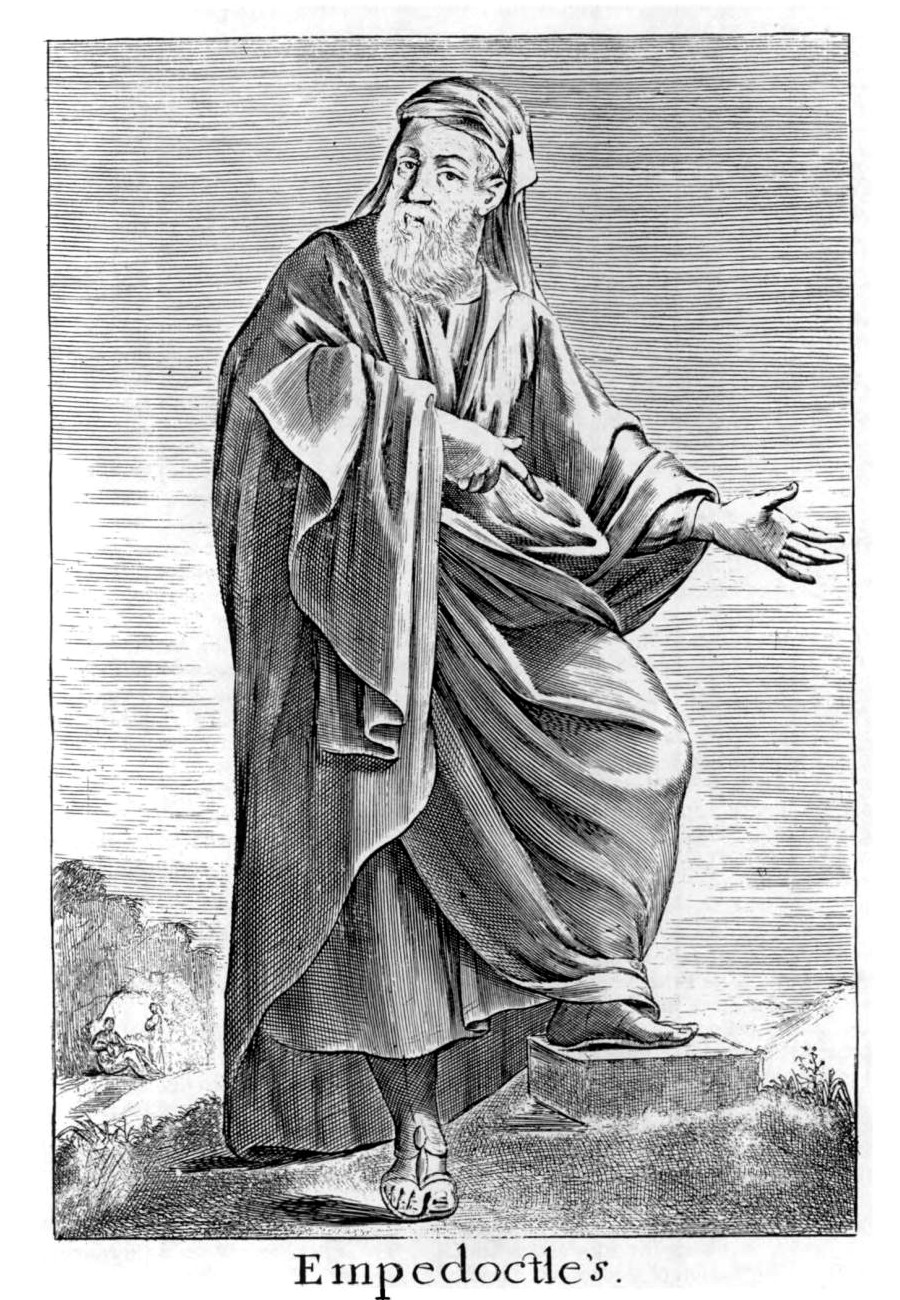
\includegraphics[width=0.4\linewidth]{./figures/empedocles.jpg}
		\caption{Empedocles \cite{Stanley1655}}
		\label{fig:empedocles}
	\end{subfigure}%
	\begin{subfigure}{0.5\textwidth}
		\centering
		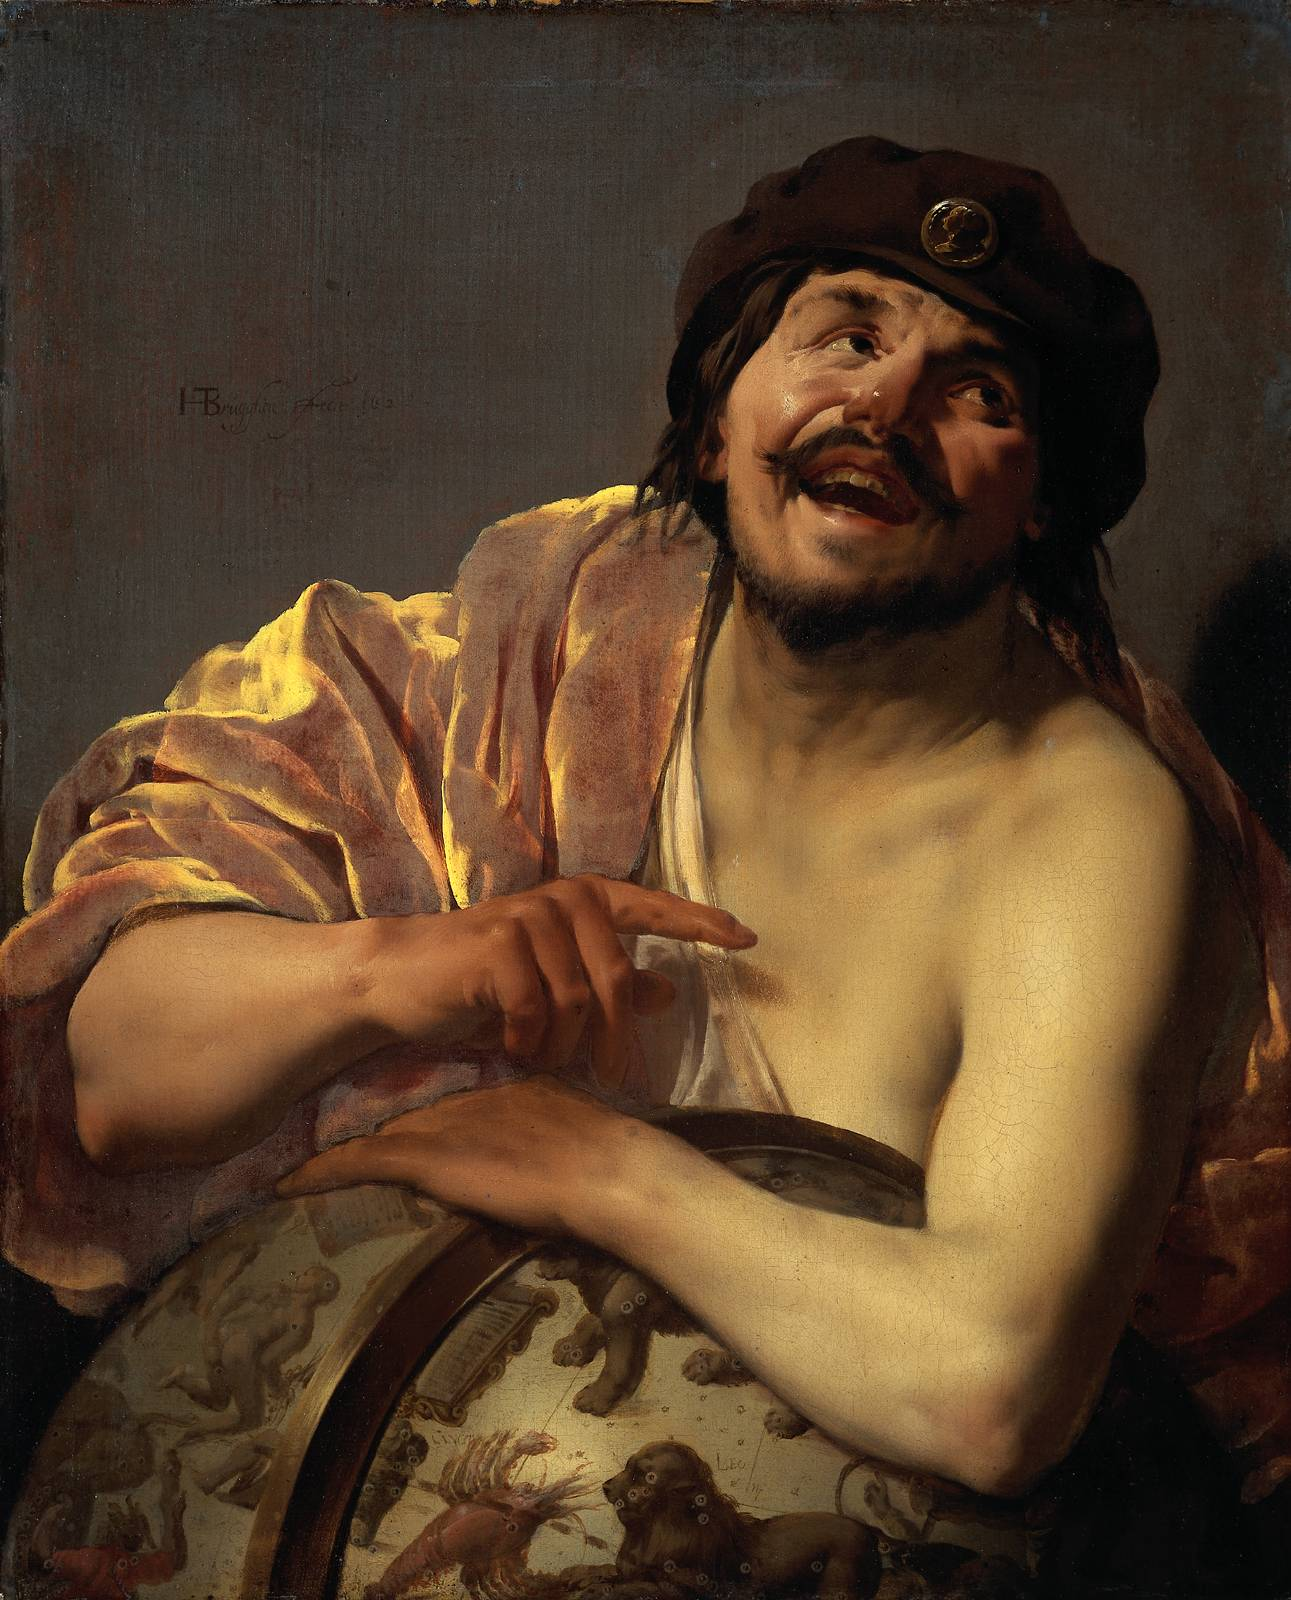
\includegraphics[width=0.4\linewidth]{./figures/democritus.jpg}
		\caption{Democritus \cite{Brugghen1628}}
		\label{fig:democritus}
	\end{subfigure}
  \caption{ 
    Two Greek philosophers, who made important philosophical contributions our
    understanding of matter. Empedocles (Panel (a)), postulated the precursor
    to the elemental theory of matter\cite{Long1949} and Democritus (Panel
    (b)), postulated the precursor to the atomic theory of matter.  
  }
	\label{fig:atomists}
\end{figure}

Democritus was part of a movement of thought which was first to make the
intellectual jump that perhaps matter was not a continuum, but instead composed
of `atomon'. `Atomon' were thought to be small and indivisible particles
building up all that is observable~\cite{Baldes1978}.  Empedocles made an
equally important philosophical stride--he posited that matter must be composed
of elemental primitives and that the properties of the primitives which build
up matter, influence the properties of the bulk matter itself~\cite{Long1949}.

Although Empedocles' `periodic table' was only composed of Earth, Water, Fire,
and Air, the idea that some unseen transmutation of elemental forces might
generate observables in nature was an important step forward. This was the
first time that humans considered that underlying structure in matter might
influence the bulk properties of matter. Proto-scientists were beginning to
generate models which derived our complicated observations from simpler forms.

\clearpage
\section{The Scientific Revolution}

Thanks to the mathematical foundations laid out by the minds of the Islamic
Golden Age (8th century - 13th century), Europe was well poised to reignite the
flames of scientific inquiry during the post Renaissance Scientific
Revolution~\cite{Alexakos2005} (17th - 18th centuries), following a renewed
interest the ideas of Greek philosophers after the dark ages.

The Scientific Revolution represented an unprecedented period of growth in
science, thanks the foundations laid during the Italian Renaissance and
emergence of British Empiricism~\cite{Cowley1968}.

\begin{figure}[ht]
	\centering
	\begin{subfigure}{.5\textwidth}
		\centering
		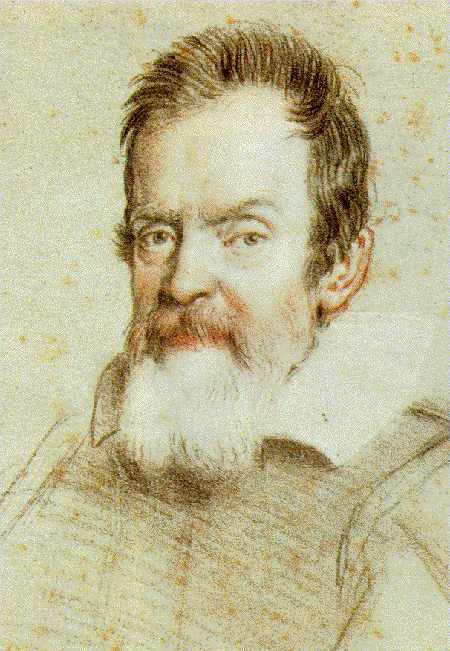
\includegraphics[width=0.4\linewidth]{./figures/galileo.jpg}
		\caption{Galileo \cite{Leoni1624}}
		\label{fig:galileo}
	\end{subfigure}%
	\begin{subfigure}{0.5\textwidth}
		\centering
		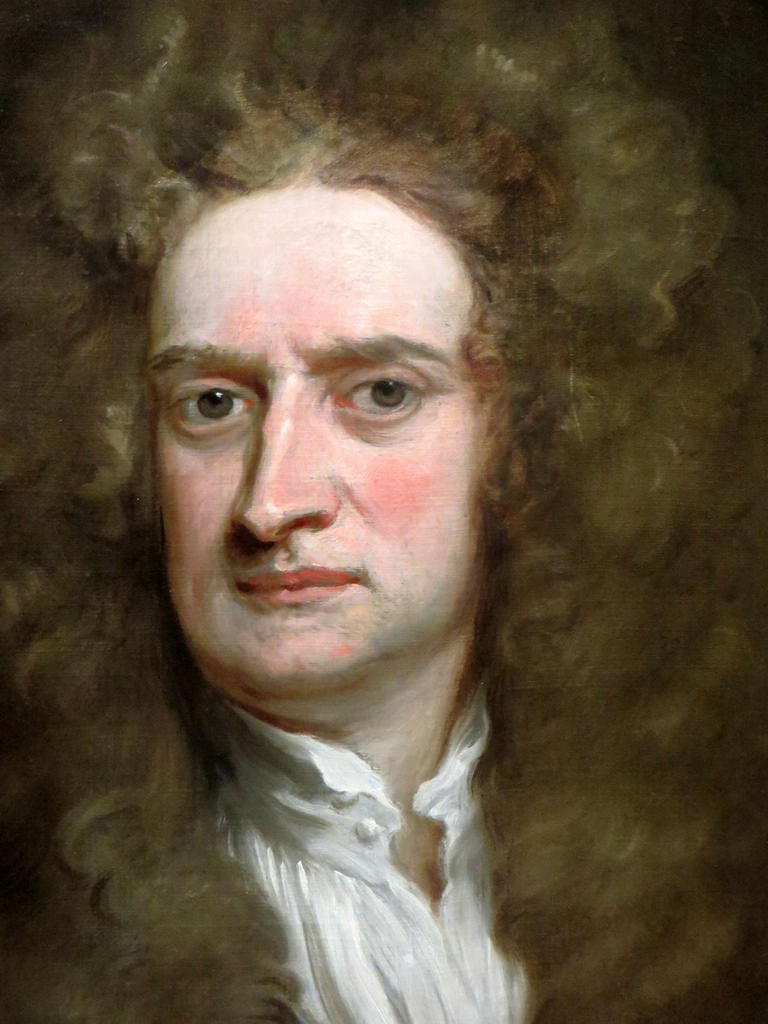
\includegraphics[width=0.4\linewidth]{./figures/newton.jpg}
		\caption{Newton}
		\label{fig:newton}
	\end{subfigure}
	\caption{ 
    Giants in the age of Empiricism, Newton (Panel (a)) and Galileo (Panel (b))
    both made foundational contributions to Physics.  Galileo lived in Italy,
    born in 1564 and dying in 1642. Newton lived in England from 1642 until his
    death in 1727
	}
	\label{fig:newtongalileo}
\end{figure}

\subsection{Galileo Galilei}

Coming at the tail end of the Italian Renaissance, Galileo brought us into the
age of Scientific Revolution.

While Galileo is best known for his work in Observational Astronomy, his
importance to science extends beyond this. During his years in exile for his
controversial views regarding the heliocentric universe, he produced some of
his most important scientific work in kinematics~\cite{Hall1965}. What made
this work remarkable is the care that Galileo took in merging mathematical
modeling with well designed experimentation. This methodical approach to
inquiry laid the foundation for the scientific method, which others would
refine. 

Galileo's formalization of the scientific method inexorably set science on a
course to delving deep into the nature of matter and the laws of nature.

\subsection{Isaac Newton}

Fittingly born in the same year as Galileo's death, Isaac Newton would carry on
Galileo's legacy of rigorous mathematical modeling mixed with experimentation.
Perhaps no other scientist has touched so many different aspects of physics,
from theories of propagation of light, to celestial mechanics, to mathematics,
and kinematics.

Newton's Principia is arguably the most important scientific work ever
published.  It opened the doors of the universe in a way that nobody has since
duplicated--Newtons' laws of motion are still taught in school today, and
applied in real scientific contexts, providing the basis for the NASA space
exploration program. Although Newton's models for motion have since been shown
to be inaccurate at the smallest and largest scales, they still provide
startlingly accurate predictions at intermediate scales.

One particularly prescient theory of Newton's was his corpuscular theory of
light. Although not his most influential theory by far, the idea that an
apparently continuous medium such as a beam of light might be made of small
packets of energy (corpuscles) turned out to be partially
right~\cite{Stuewer1970}, and gained an interesting new context with the
emergence of Quantum Mechanics in the early 20th century.

Newton's theories, and contributions to science are enormous, and have moved us
deeper still into the underpinnings of matter. It would not be until roughly 200
years after his death, in the 19th century, that we finally can take the first
steps into the world of the atomic, and sub-atomic: the world of the proton. 

\clearpage
\section{Atomic Theory}

On the shoulders of giants such as Newton and Galileo, science finally came to
know the tool which has been indispensable to modern particle physics:
scattering. Rutherford and Thompson both carried out the most important
scattering experiments in modern science. These experiments provided us with
the first hints of a hidden, quantum world. It would not be until the 20th
century that these important experiments would be fully contextualized with a
theory of quantum scattering.

Scattering experiments offer a very powerful method where one uses a well known
initial state of matter (typically in the form of a beam) and allows this beam
to interact with an unknown configuration of matter. The final state of the
target and scattered beam are measured. With a careful study of the kinematics
of the scattered beam, one can create models that offer a peak into the
structure of the target matter. As we journey down further in scale, matter
begins to look quite different.  In fact, the models we use are scale dependent,
Figure~\ref{fig:scale_of_matter}. Thomson (Figure~\ref{fig:thomsonrays}), and
Rutherford (Figure~\ref{fig:rutherford}) began to see matter as collections of
atoms.  Soon, nuclei were discovered to be divisible into protons an neutrons,
which in turn were discovered to be composed of a sea of quarks and gluons.

\begin{figure}[ht]
	\centering
	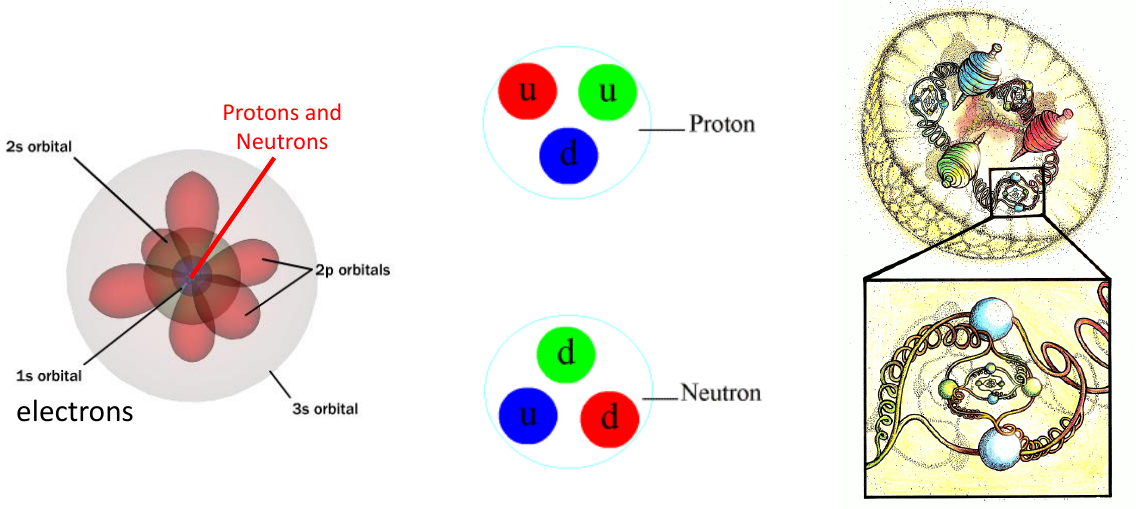
\includegraphics[width=\linewidth]{./figures/scale_of_matter.png}
	\caption{
    Matter at an atomic scale~\cite{Freudenrich2001} (left), intermediate
    nuclear scale~\cite{Manisearth2010} (center), and the sub-nuclear partonic
    scale (right)~\cite{Morreale2009}
	}
	\label{fig:scale_of_matter}
\end{figure}

\subsection{John Dalton}

While many had postulated the existence of atoms, the first evidence based
theory which suggested the existence of atoms was produced by John Dalton in the
early 19th century. Dalton made an important conceptual leap to relate the
existence of stoichiometric ratios in chemistry to the presence of small,
individual functional units in his experiments with chemical reactions.
Dalton's realization was only made possible due to his careful accounting of
reactants in his experiments.

However, humanity had to wait for Einstein's 1905 theory on Brownian Motion to
be experimentally verified by Jean Perrin to obtain the first limits on the mass
and size of atoms that Dalton's atomic theory predicted~\cite{Patterson200750}.

\subsection{J.J. Thompson}

\begin{figure}[ht]
	\centering
	\begin{subfigure}{.4\textwidth}
		\centering
		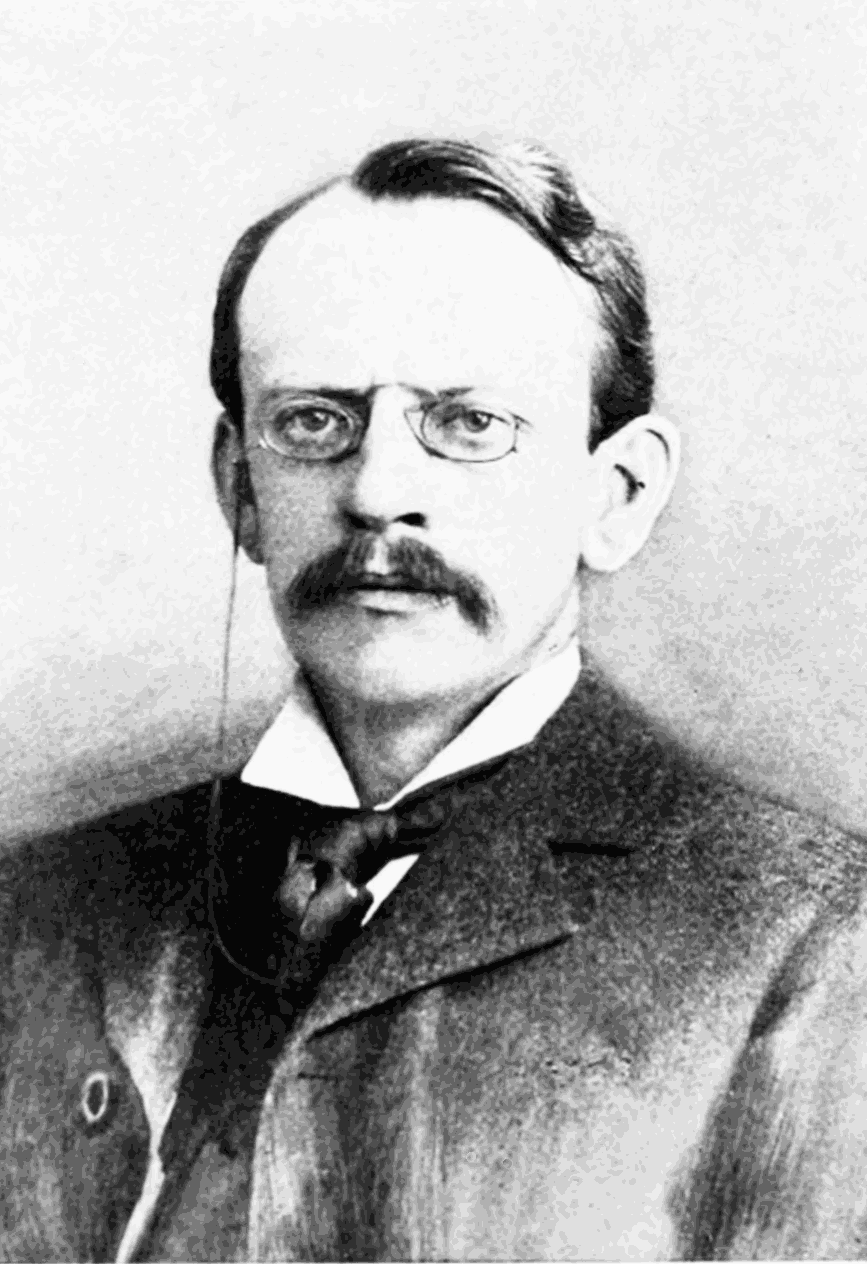
\includegraphics[width=0.4\linewidth]{./figures/jjthomson.png}
		\caption{J.J. Thomson  \cite{PopularScience1899}}
		\label{fig:thomsonportrait}
	\end{subfigure}%
	\begin{subfigure}{0.6\textwidth}
		\centering
		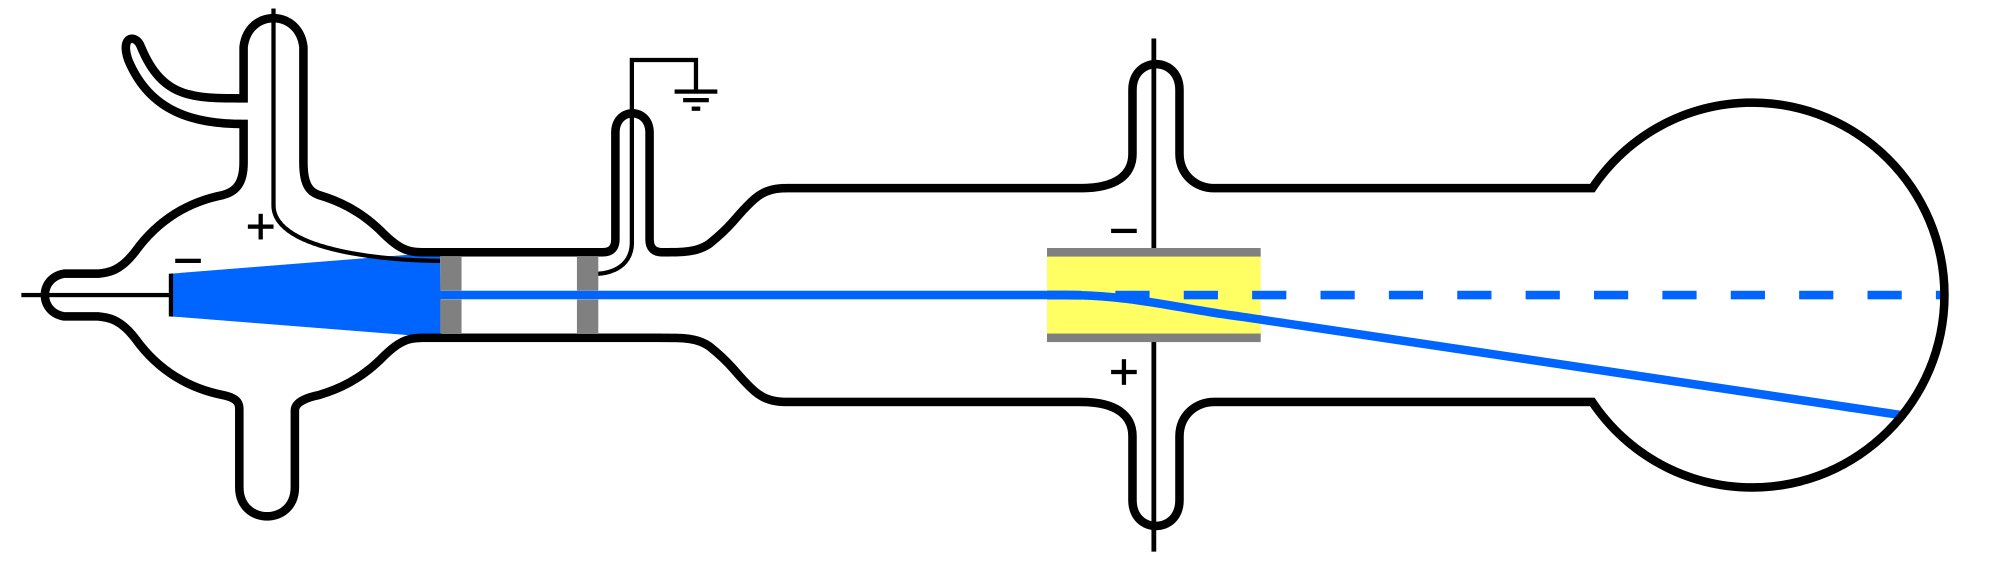
\includegraphics[width=0.4\linewidth]{./figures/cathoderaytube.png}
		\caption{Cathode Ray Tube  \cite{Kurzon2010}}
		\label{fig:thomsoncathode}
	\end{subfigure}
	\caption{ 
		Left: J.J. Thomson, who showed that cathode ray tubes were in fact producing
		the first observed subatomic particle: the electron. Right: A cartoon of
		Thomson's cathode ray tube setup. Electrons would be deflected by a magnetic
		field, sent from cathode to anode.
	}
	\label{fig:jjthomson}
\end{figure}

Thomson (Figure~\ref{fig:jjthomson}) would discover that atoms are not the
smallest indivisible piece of matter. In his landmark experiment, he used
cathode ray scattering experiments to show that cathode rays were in fact
subatomic particles. He showed these cathode rays were identical to particles
given off by the photoelectric effect. He discovered that these were the same
particles responsible for electric current.  Scientists began to wonder: if
atoms were not the smallest piece of matter, then perhaps atoms themselves
might not be `indivisible' as previously thought \cite{nobelthomson2014}.

\subsection{Ernest Rutherford}

\begin{figure}[ht]
	\centering
	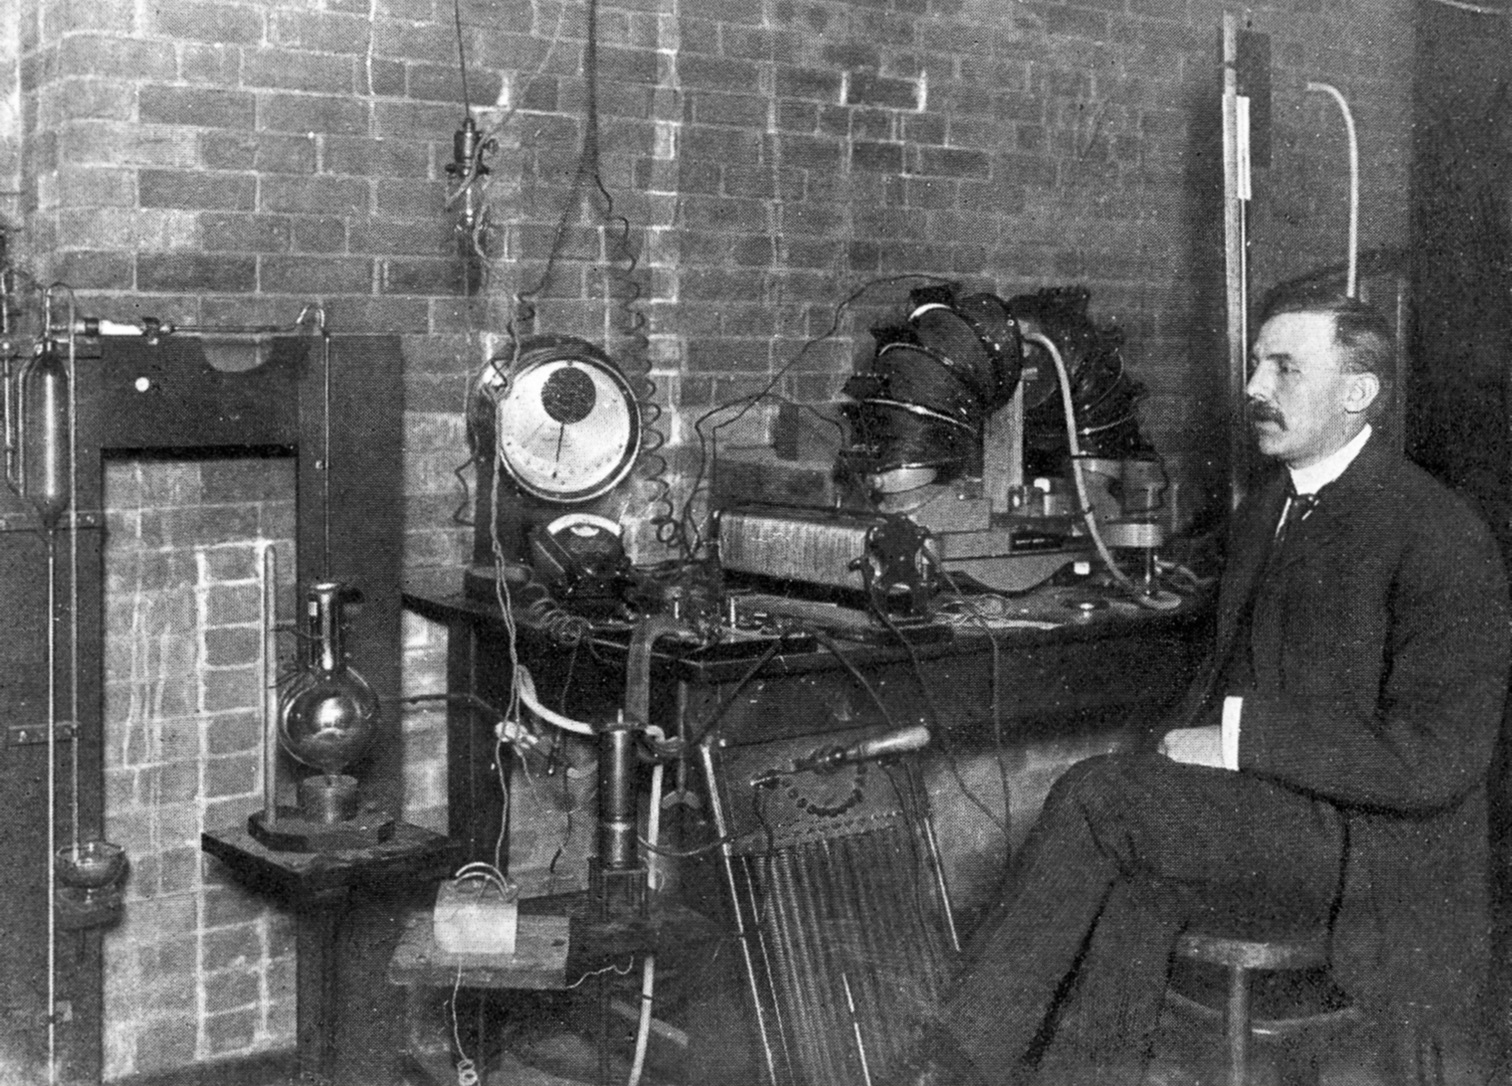
\includegraphics[width=0.6\linewidth]{./figures/ernestrutherford.jpg}
	\caption{Ernest Rutherford, in his lab.  \cite{Eve1939}}
	\label{fig:rutherford}
\end{figure}

Ernest Rutherford (Fig~\ref{fig:rutherford}) was the first to show that atoms
themselves had underlying structure and consisted of a small dense center.  He
had discovered the nucleus.

\begin{figure}[ht]
	\centering
	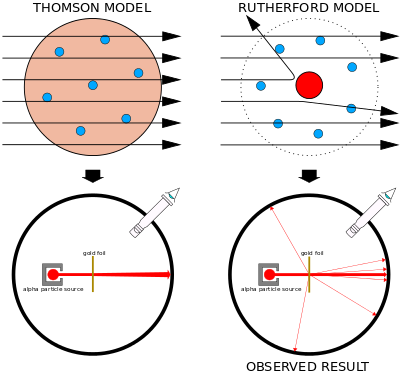
\includegraphics[width=0.6\linewidth]{./figures/geiger_marsden.png}
	\caption{
		Ernest Rutherford's historic experiment, showing (top right) that atoms were
		composed of a small dense nucleus, in contrast to Thomson's `pudding model'
		of homogeneous charge (top left). The experiment, (bottom left and right)
		contrast the expected results (bottom left) against the observed results
		(bottom right)  \cite{Kurzon2014}.
	}
	\label{fig:geigermarsden}
\end{figure}

Rutherford's work with radioactivity was of fundamental importance. He
discovered and classified both alpha-particle radioactivity and beta-particle
radioactivity. Further studies into these types of nuclear radiation would
unlock the nucleus of atoms through the work of future scientists.

After his discovery of the proton, Rutherford proposed a planetary model for the
nucleus. While this model was eventually shown to be wrong, it shifted paradigms
from the pudding model of atoms to the more familiar nucleus + electron model.
This shift eventually led to the emergence of Quantum Mechanics.

Rutherford's work helped push us out of the cocoon of classical mechanics into
the world of the quantum mechanics--scientists would soon find that the nucleus
is not just a dense concentration of charge, but a probabilistic structure, with
rich sub nuclear structure.

\clearpage
\section{Early Quantum Theory}

During Rutherford's time, experiments were already underway investigating
modeling light as a wave phenomena. This was in contrast to Newton's
(unverified) corpuscular theory of light. The argument whether light was
wave-like or particle-like eventually lead to a classical field theory
describing light as electromagnetic radiation. Max Planck proposed theories
which required the quantization of light~\cite{Planck1901}.  Einstein would show
that light is indeed quantized into packets of energy in his analysis of the
photoelectric effect. The nascent atomic theory of matter hinted at a hidden,
quantized world.

\begin{figure}
	\centering
	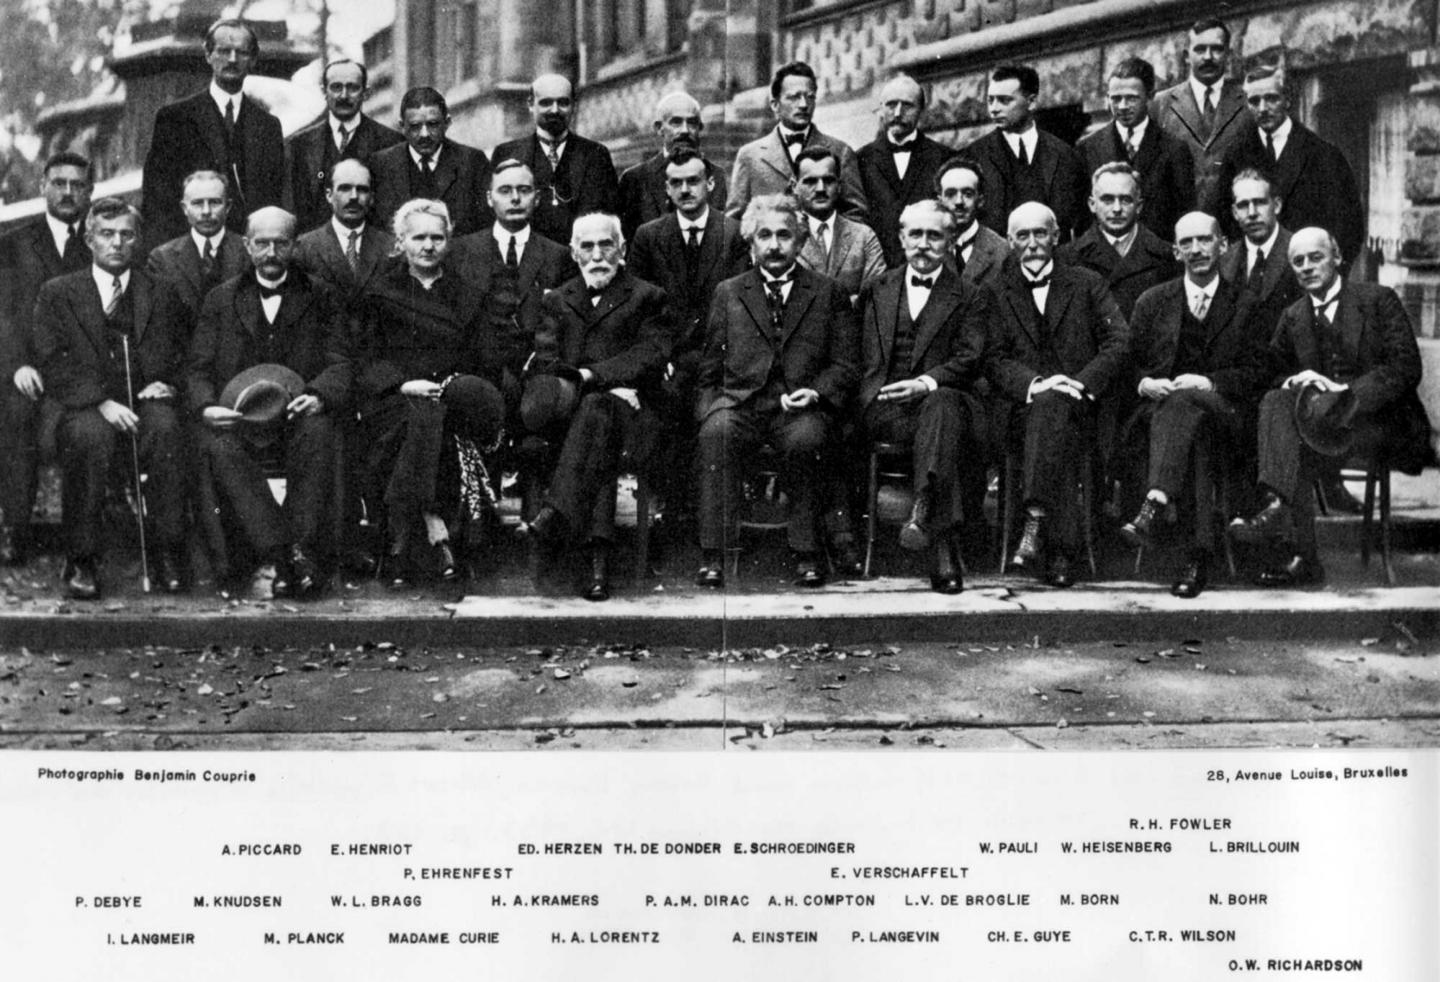
\includegraphics[width=\linewidth]{./figures/solvay.jpg}
	\caption{
		The attendees of the Solvay Conference in Brussels, 1927
		 \cite{BenjaminCroupie1927}.
	}
	\label{fig:solvay}
\end{figure}

At the 1927 Solvay Conference in Brussels(Figure \ref{fig:solvay}) an
unprecedented gathering of some of the most important figures in modern physics,
built the foundations of what would become quantum mechanics. These scientists
defined the nature and rules of quantum mechanics--the weird model which
accommodates a wave-particle duality of matter. 

It was found that not only light possesses this wave-particle duality, but also
the particles that make up atoms. These models were formalized by Paul Dirac,
David Hilbert and John Von-Neumann.

Further refinements and additions to quantum mechanics gave birth to quantum
field theory. Early quantum models were very successful at describing static
particles trapped in static potentials. Scientists could predict exactly
observed atomic emission spectra. But, more work was needed to understand the
relationship between electrical currents, light and magnetism.  These concepts
were all related by James Clerk Maxwell~\cite{Maxwell1865} in the latter half of
the 19th century, but had yet to receive a quantum-treatment.

Dirac was first to create a model for describing the electron, its behavior in
electromagnetic fields, and photon emission and absorption. Dirac's models were
fully relativistic~\cite{Dirac}. Dirac's model was so successful, that it would
become the basis for what we now call quantum electrodynamics.  Much of the
mathematical formalism was reused to describe other field theories. Field Theory
is the ultimate language used in modeling and describing the structure of
matter--including the insides of a proton. 

\begin{figure}[ht]
	\centering
	\begin{subfigure}{.4\textwidth}
		\centering
		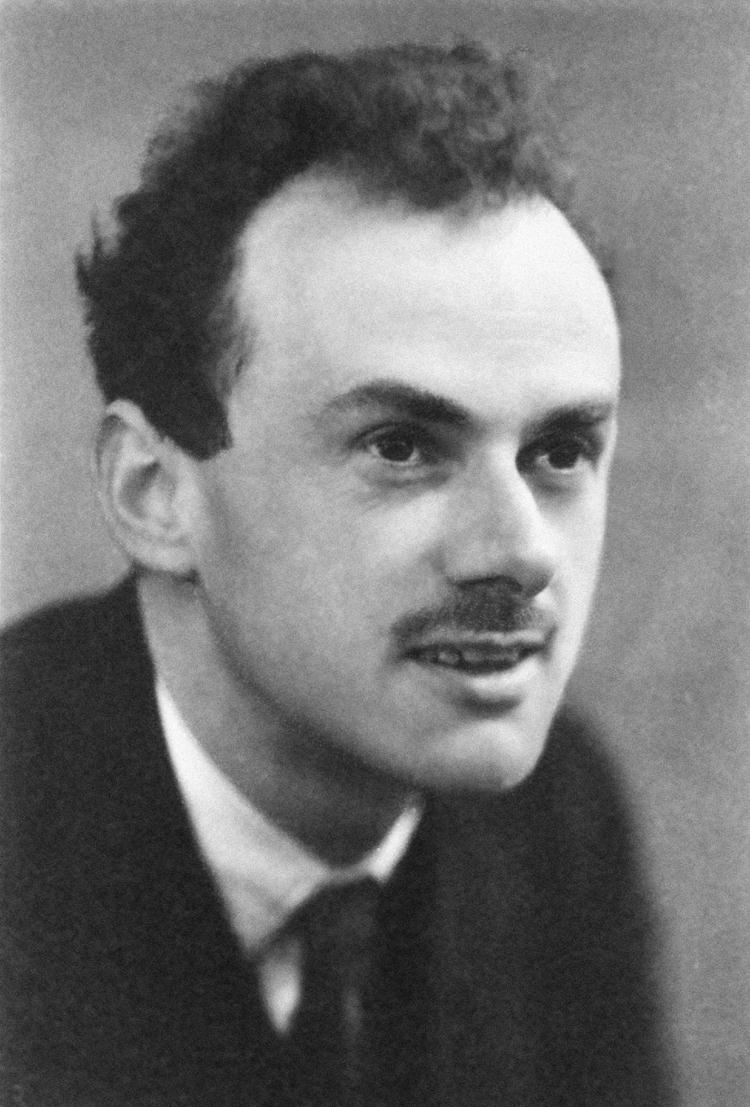
\includegraphics[width=0.4\linewidth]{./figures/pauldirac.jpg}
		\caption{Paul Dirac, 1933  \cite{NobelFoundation1933}}
		\label{fig:pauldirac}
	\end{subfigure}%
	\begin{subfigure}{0.6\textwidth}
		\centering
		\begin{equation}
			\left(\beta mc^2 + c\left(\sum_{n \mathop =1}^{3}\alpha_n p_n\right)\right) \psi (x,t) = i \hbar \frac{\partial\psi(x,t) }{\partial t}
		\end{equation}
		\caption{The `Original Form' of the Dirac Equation}
		\label{eq:diracquation}
	\end{subfigure}
	\caption{ 
		Paul Dirac, next to his original formulation of the Dirac Equation,
		describing the wave function for an electron with rest-mass $m$, in terms of
		its space-time coordinates. Dirac's equation has been expressed free of any
    defined basis.
	}
	\label{fig:thomsonrays}
\end{figure}

Dirac's work successfully merged relativity into his wave equations describing
the motion of particles. He additionally incorporated the spin (i.e. Dirac
Spinors) of these particles. The inclusion of spin allowed for the most precise
predictions ever to be made for hyperfine divisions in the atomic
spectra~\cite{Dirac}.

In Dirac's time, the proton was already known to reside in the enigmatic
nucleus. However attempts to use Quantum Electrodynamics to describe the state
of the nucleus failed. It was clear that there was a very strong force holding
together the positively charged protons of a nucleus. This force would have to
be far stronger than the electromagnetic repulsion felt by the positively
charged particles in such close proximity. Further complicating an understanding
of the nucleus is the fact that as the length scale of probing decreases, the
energies probed increase. This fundamentally makes the nucleus a relativistic
object. Physics would once again forge ahead in attempting to understand the
inner workings of the nucleus.

\clearpage
\section{Early Particle Physics and The Eightfold Way}

The hydrogen atom and its spectra was well-modeled with quantum mechanics by the
end of the early 20th century. However, attempts to study Helium were not as
successful. By 1932, when James Chadwick turned a beam of helium particles (at
that time only known as $\alpha$ particles) on a sample of Beryllium, he
observed that neutral, non-ionizing, penetrating radiation was produced
\cite{Krauss2015}.  Photons were ruled out as possible candidates, leading to
the discovery of the neutron. Protons and neutrons were hypothesized by
Heisenberg to both be the same state of a new conceptual particle, the
nucleon~\cite{Heisenberg1952}. In the same year, Carl Anderson discovered the
positron. 

By 1934, Hideki Yukawa (Fig.~\ref{fig:hidekiyukawa}) had created an effective
field theory for interactions of `elementary particles' (at this time, thought
to be protons and neutrons). He predicted the existence of mesons, and wrote
down an effective field theory which described how protons and neutrons bind
together in the nucleus \cite{Yukawa1935}. 

Though non-relativistic quantum mechanics was mostly complete by 1934,
scientists were already hard at work incorporating relativistic corrections to
the theory. Experiments with cosmic rays soon revealed the existence of muons
and the first observation of mesons.

\begin{figure}[ht]
	\begin{center}
		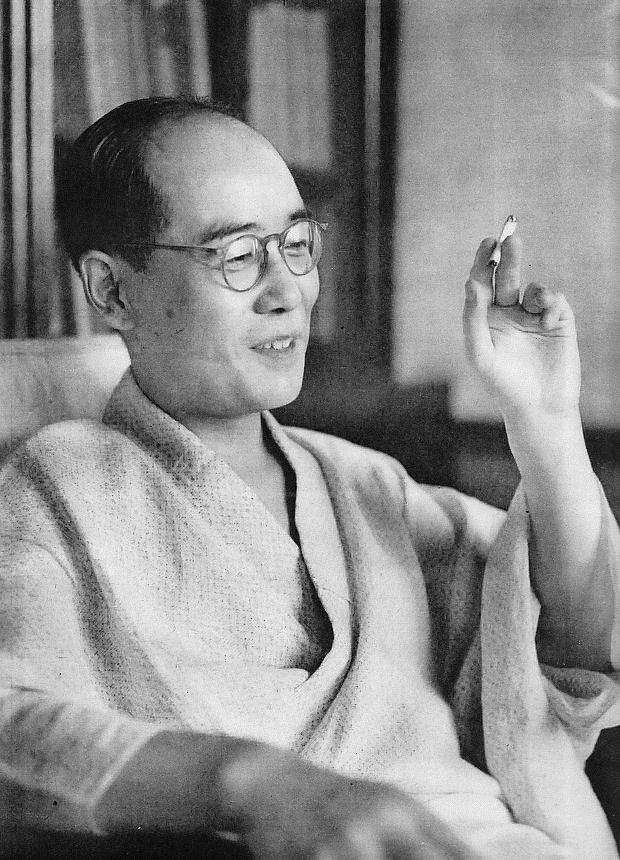
\includegraphics[width=0.5\linewidth]{./figures/hidekiyukawa.jpg}
		\caption{
			Hideki Yukawa, the first Japanese Nobel Laureate and publisher of
			influential research on the theory of mesons, and other elementary
			particles  \cite{YukawaPhoto1952}.
		}
		\label{fig:hidekiyukawa}
	\end{center}
\end{figure}

Three separate paths eventually lead to the development of particle
accelerators. To date, these massive machines provide the best apparatus in
physics to probe nuclear structure. These accelerators are an outgrowth of ever
more intense Rutherford-style experiments. An array of technologies have
supported this growth: Tandem Van-Der-Graaf generators, resonant acceleration
techniques, RF linacs, and betatron accelerators \cite{Bryant1994}.

By the 1950s a cornucopia of strange new particles had been discovered, both
matter and antimatter. Neutrinos were proposed as a means of understanding
`missing energy' observed in some scattering experiments. Mesons such as Kaons
($K$), Pions ($\pi^+,\pi^-,\pi^0$), and Lambdas ($\Lambda$) were well
understood.  Physicists were doing nuclear chemistry, attempting to work out how
quickly some particles decayed, and what decays were allowed or forbidden.
Science entered an age of nuclear alchemy.

``Strange'' particles were discovered ($K$ and $\Lambda$), so called because in
bevatron experiments, they were produced in great quantities, but were slow to
decay, unlike the faster $\pi$ decay. Gell-Mann proposed that this strangeness
in matter was due to a new quantum number (he called it `strangeness'). The name
stuck~\cite{Gell-Mann1953}, \cite{Gell-Mann1956}, \cite{Krauss2015}.

The introduction of new conserved quantities and the vast proliferation of
particles was an exciting puzzle for physicists to unravel. The subatomic world
of the 1950s was confusing and complex. In his book, \textit{The God Particle},
Leon Lederman recalled his adviser (Enrico Fermi) frustratedly remarking `Young
Man, if I could remember the names of these particles, I would have been a
botanist'.  At this time the number of mesons and baryons that had been
discovered were at least in the dozens, if not more.

While the use of particle accelerators were speeding along the scientists' quest
to understand structure of matter, one particular invention truly revolutionized
the field--the bubble chamber (Figures~\ref{fig:bubble_chamber} and
~\ref{fig:bubble_tracks}).

The bubble chamber is essentially a large vat of supercritical fluid which could
easily be caused to boil with small perturbations. This feature was exploited,
by positioning a bubble chamber in a magnetic field (to cause charged tracks to
bend) near the interaction point between a particle beam and a fixed target. The
bubble chamber itself was sometimes the target--since a popular liquid to use
was hydrogen. 

\begin{figure}[ht]
	\centering
	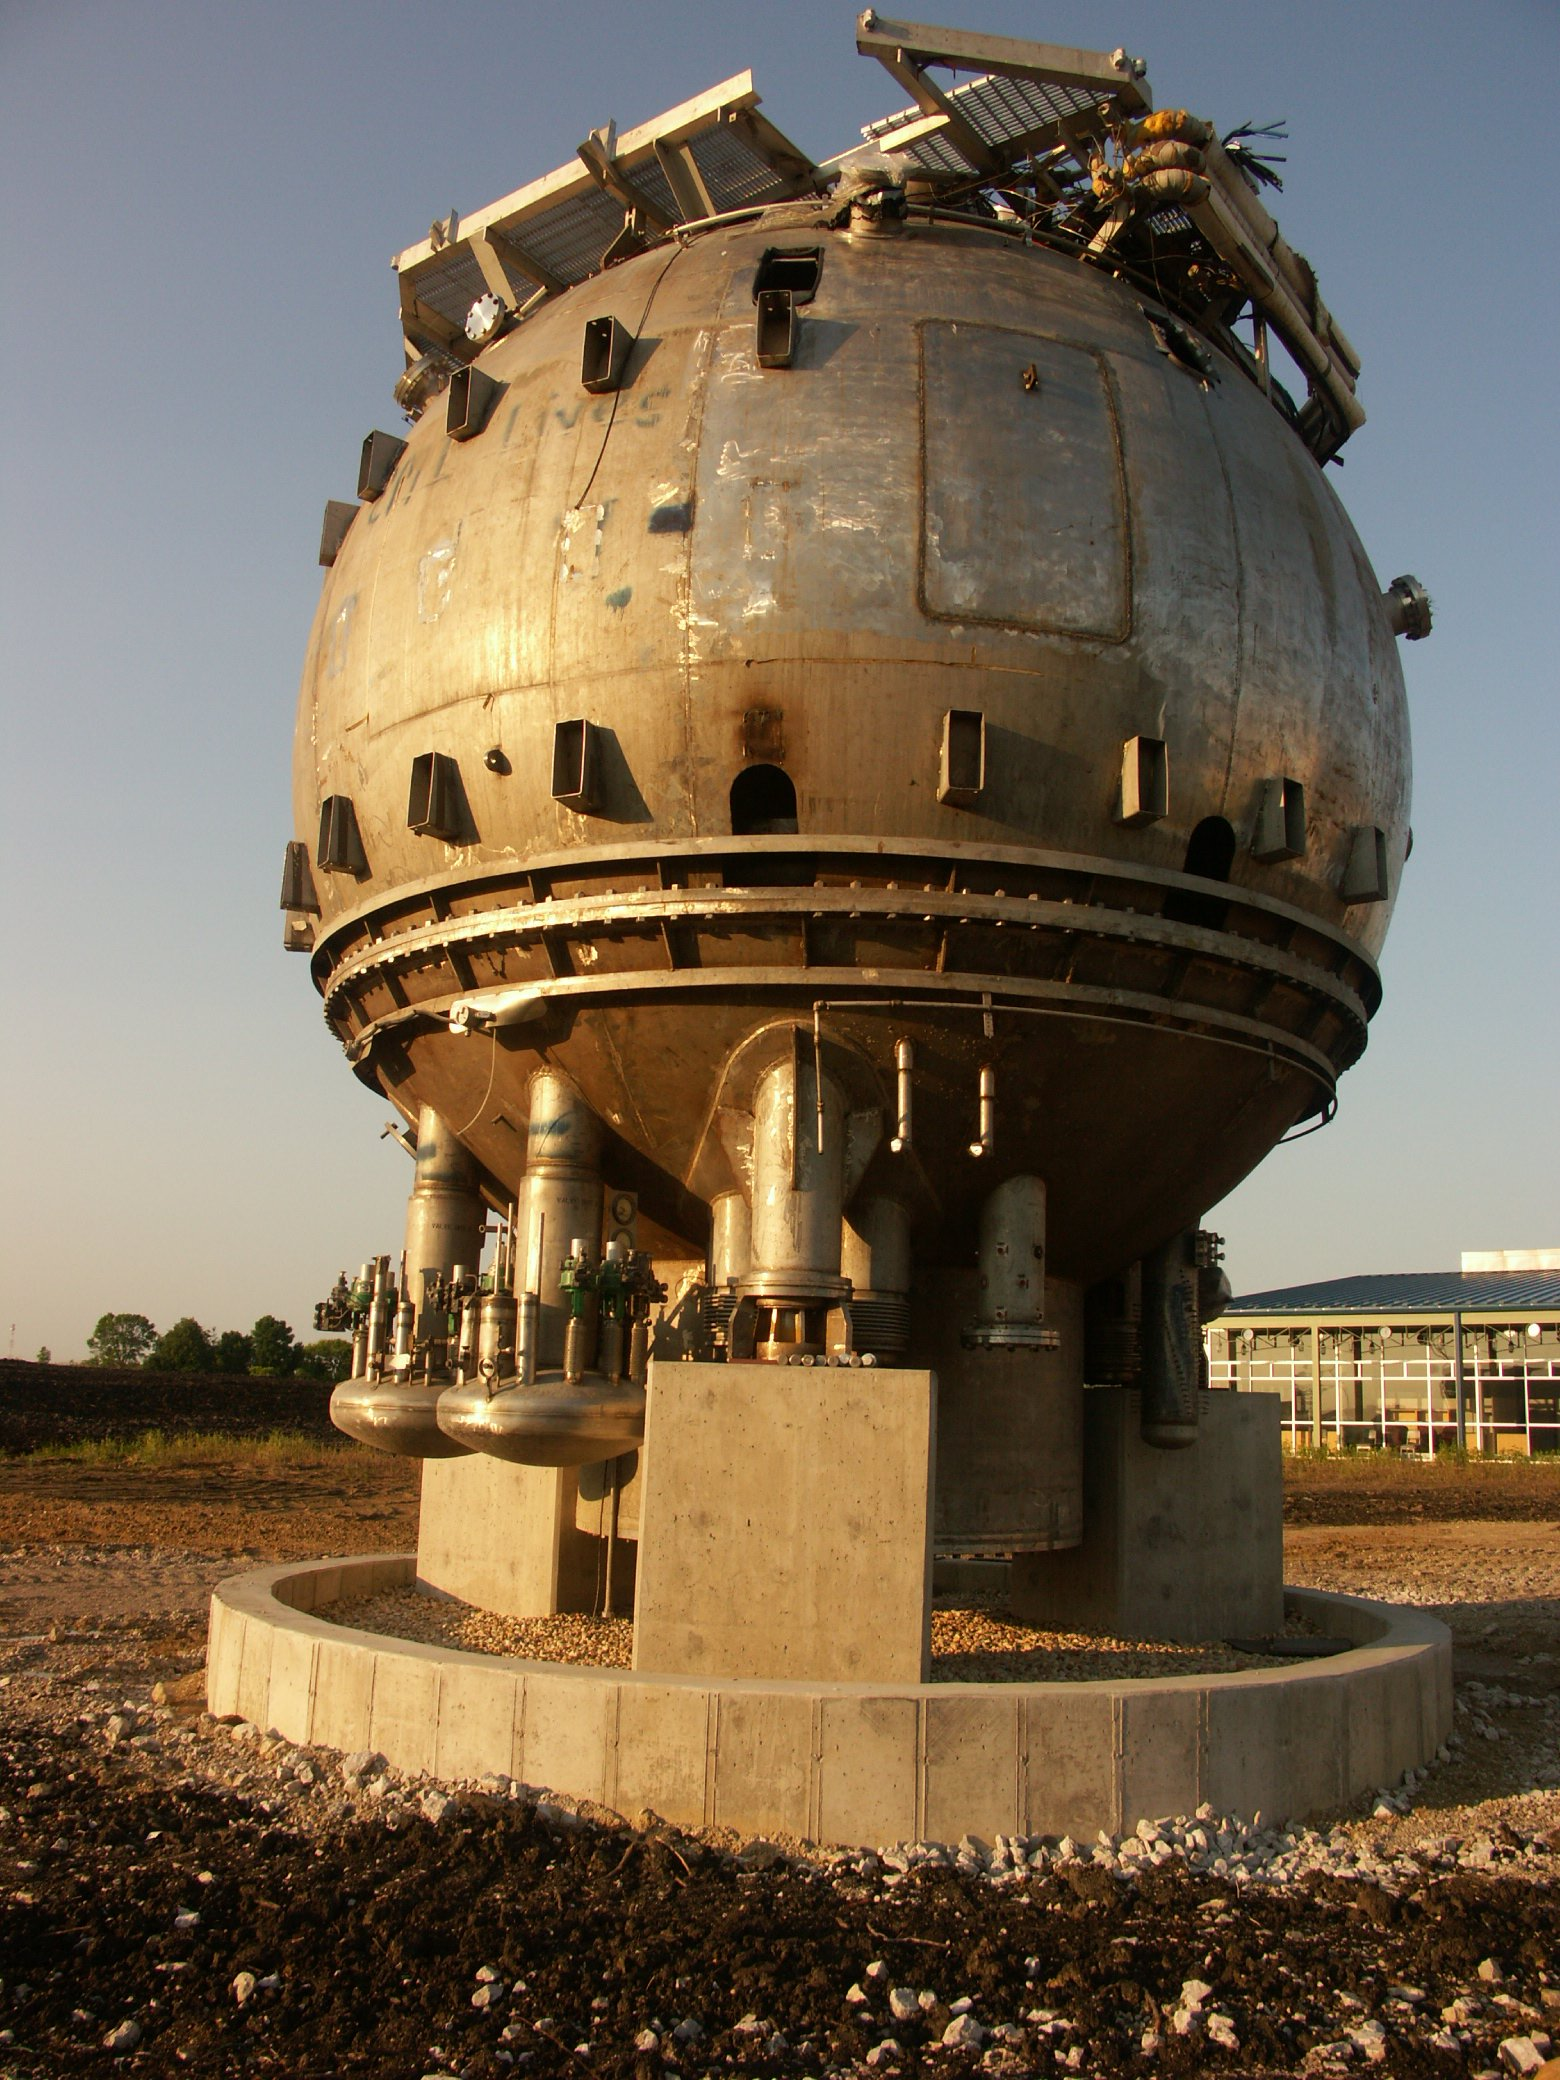
\includegraphics[width=0.5\linewidth]{./figures/bubblechamberfnal.jpg}
	\caption{An old bubble chamber, once used at Fermilab,
	 \cite{FNALBubbleChamber2005}}
	\label{fig:bubble_chamber}
\end{figure}

Invented by Donald Glaser in 1952, the bubble chamber was `perfected' by Luis
Alvarez when he helped to develop a version which could be used with liquid
hydrogen. Hydrogen was desirable as a target and medium due to its simple
structure. This led to cleaner results, unlike the original medium Ether.
Additionally, using hydrogen gave physicists a convenient way to directly probe
the sub-nuclear structure of the simplest form of matter.

\begin{figure}[ht]
	\centering
	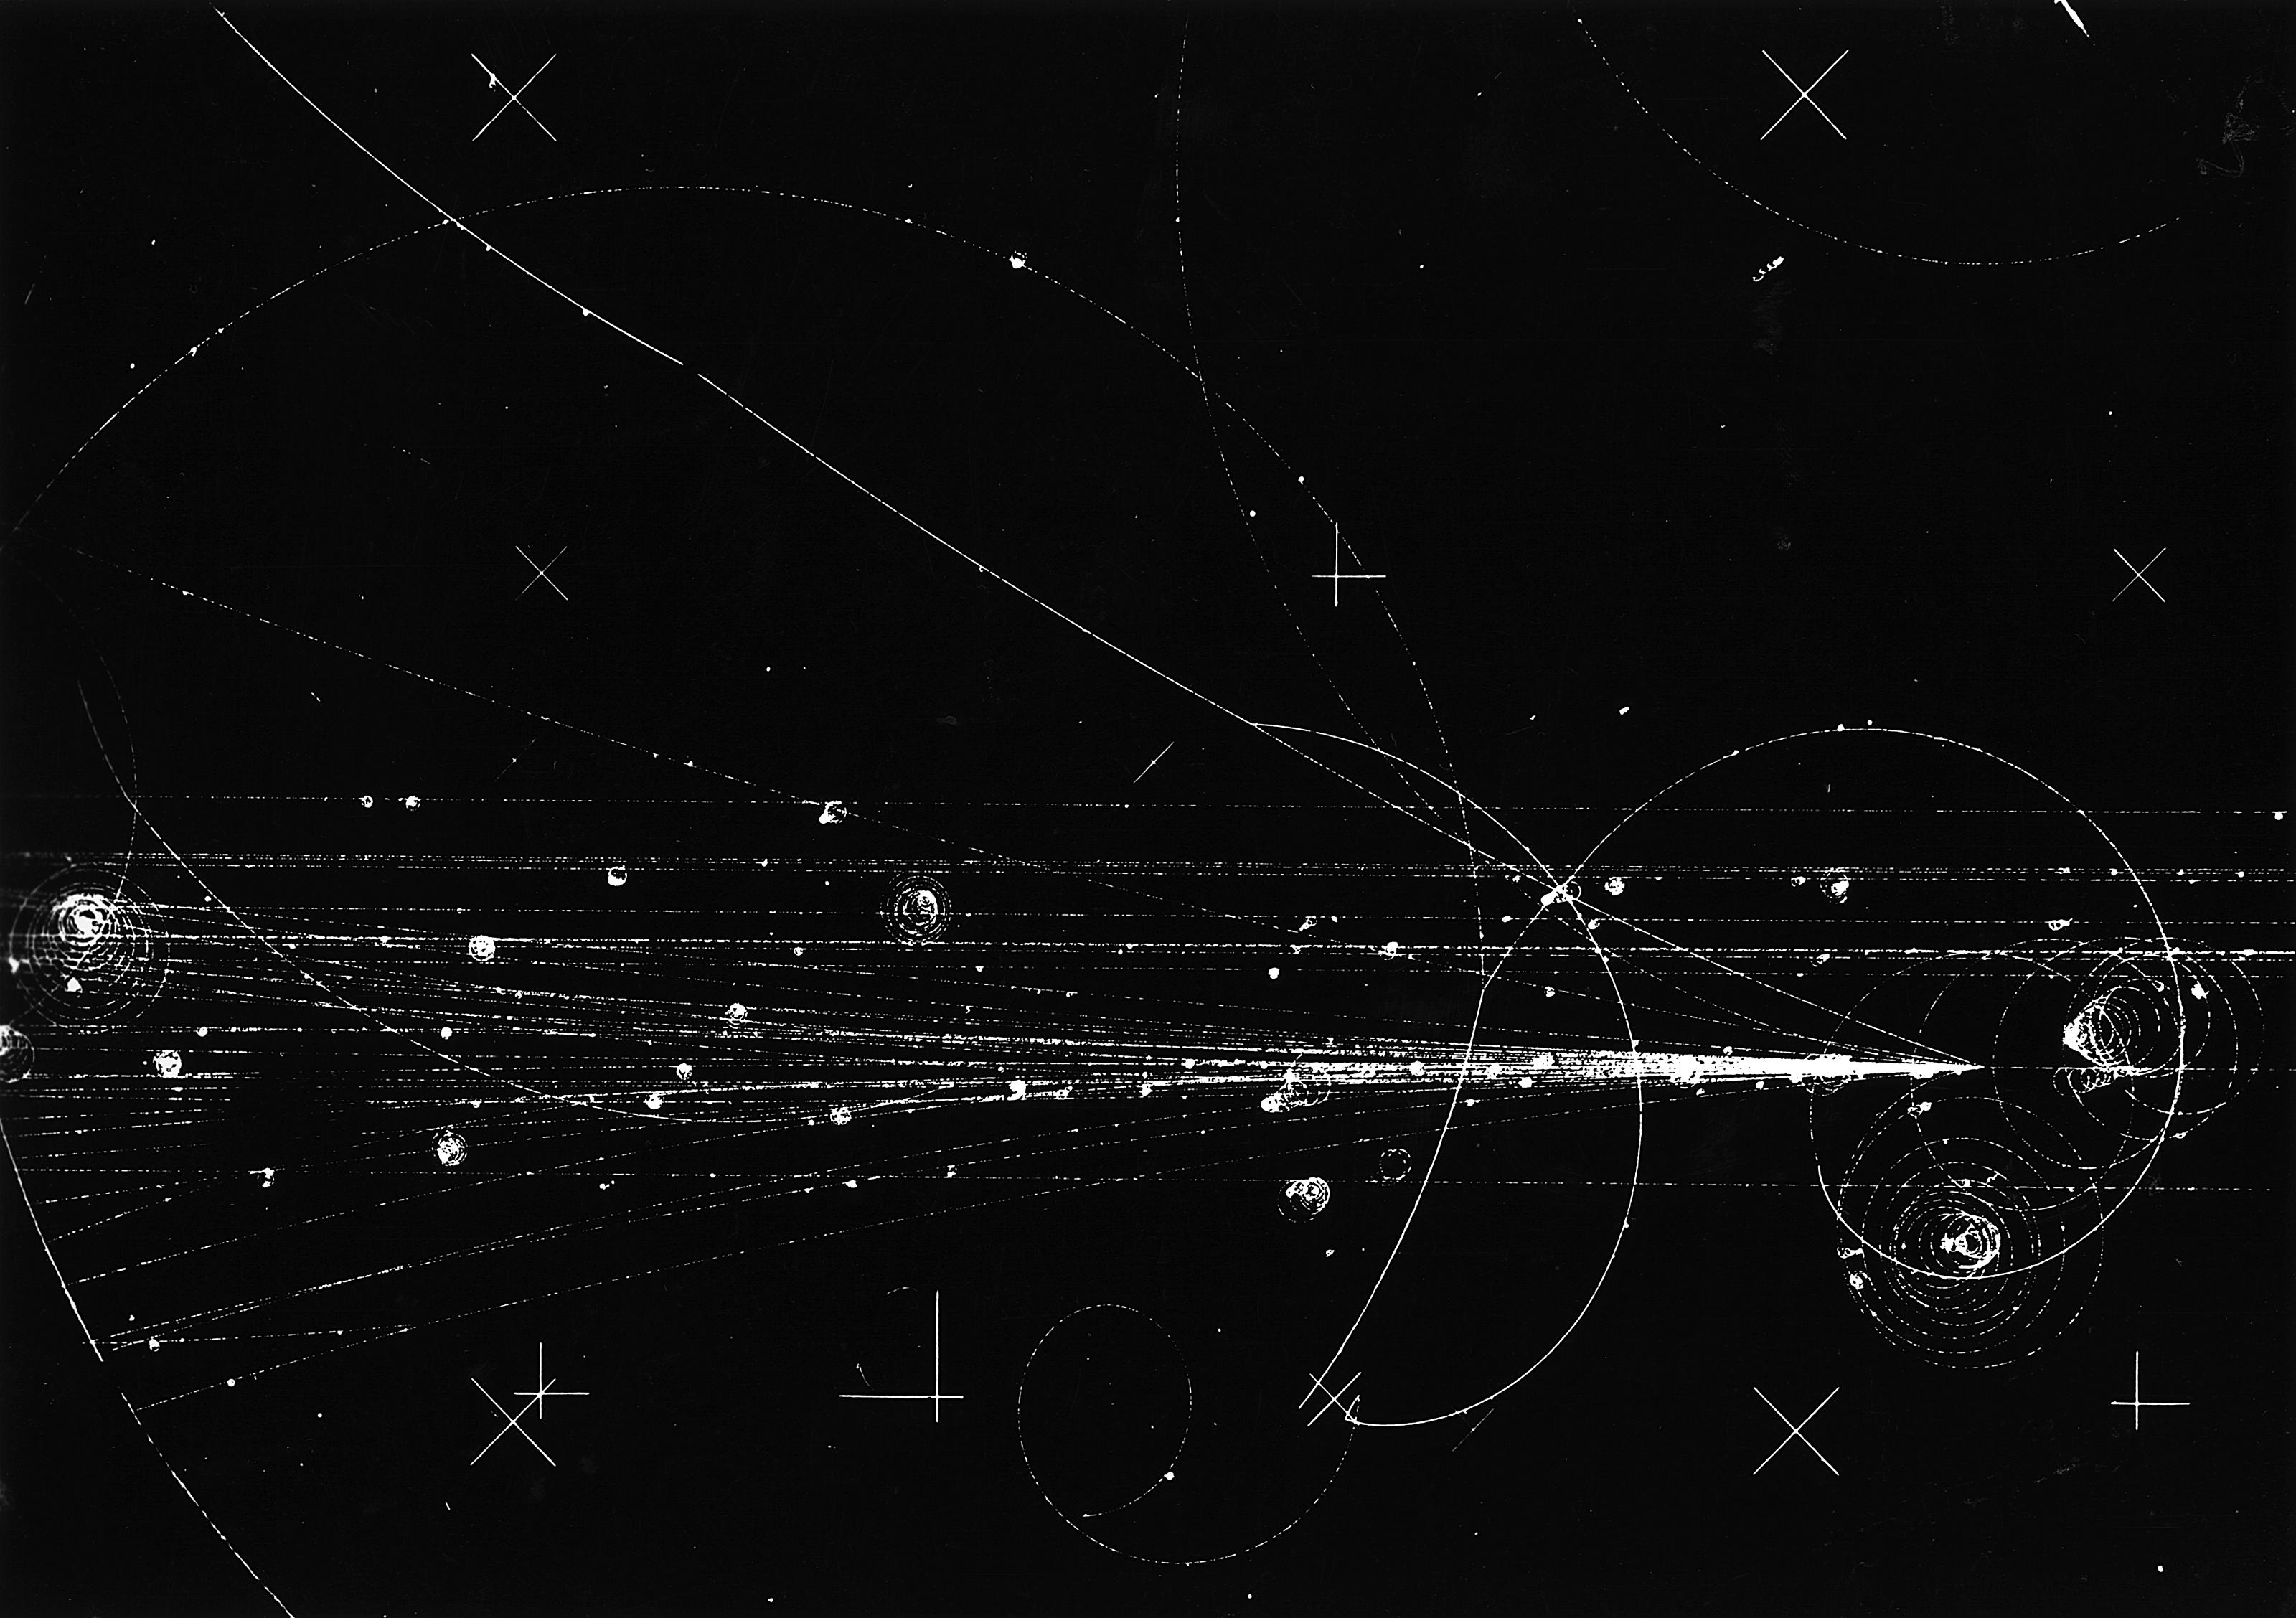
\includegraphics[width=0.5\linewidth]{./figures/bubble_chamber_tracks.jpg}
	\caption{
		An example of the photographs taken with a Bubble Chamber, in 1973.
		In this picture, we see a 300 $GeV$ proton producing particles as it travels
		through a hydrogen-filled bubble chamber at Fermilab  \cite{HD6B235}.
	}
	\label{fig:bubble_tracks}
\end{figure}

Soon after the advent of bubble chambers, physicists were able to
macroscopically image these new, exotic particles interacting with normal matter
and decaying. Novel computer techniques were developed to analyze and catalog
the massive influx of data.

A break-through came in 1961, when Gell-Mann and Nishijima recognized the
underlying symmetry of the interactions taking place and created what would be
known as `the eightfold way'. This theory created a scheme for organizing the
observed baryons and mesons according to their properties in groupings called
``octets''. These octets were in fact representations of the elements of members
of the $SU(3)$ group. Gell-Mann had discovered the underlying structure of
flavor-symmetry between the three lightest quarks--$u$, $d$, and $s$. 

Gell-Mann's quark model soon made important predictions which were later
verified, notably the existence of the $\Omega^{-}$ mesons, the ground-state
particle of the spin-$3/2$ decuplet, discovered at Brookhaven National
Laboratory. Gell-Mann formalized his quark theory of matter in 1964, however,
due to the unforeseen phenomena of color confinement, it would be several years
before evidence of quarks composing baryons and mesons was directly obtained
from deep inelastic scattering experiments.

This work directly led to the development of the quark model of matter and the
foundation of what would become the foundation of the standard model of
particles. To date, the standard model is the most successful theory describing
particles and their interactions.


\clearpage
\section{Deep Inelastic Scattering, Quantum Chromodynamics and The Parton Model}

Deep inelastic scattering experiments (Figure~\ref{fig:disschematic}) were a
natural outgrowth of Rutherford's experiment from the late 19th century.
Rutherford's scattering experiments can be modeled classically, by using a
classical potential as a scattering source. One solves as usual using an
impact parameter and potential as in central force problems.  Rutherford's
experiments were considered generally `elastic' because the target absorbed very
little kinetic energy from the projectile, and no new particles were created
from the kinetic energy of the projectile-target system.

By the late 20th century, scattering experiments became highly inelastic.
Targets would absorb a lot of kinetic energy, sometimes so much that targets
would break apart and the kinetic energy of the system would create particles.

Deep Inelastic scattering describes the process in which a high energy
interaction occurs between a projectile (often a beam) and a target (a gas, or
another beam). The process is akin to smashing to swiss-watches together to
understand how the gears fit together in synchrony to tell time. 

The interaction occurring between the target and the projectile can change the
state of the projectile and generate matter due to the high energies involved.
One can observe the state of the projectile and account for the matter which is
created.  If there are laws which govern how the state of the projectile changes
or the kinds of matter that can be created, then we can run the clock backwards
and reconstruct the initial state from the final state of the interaction.
Alternatively, the goal of deep inelastic scattering may also be to simply
measure and characterize the final state of an interaction, based on a known
initial state. This process teaches us something about nuclear structure (or
even partonic structure). In this way, one can also identify conserved
quantities, which in turn suggest physical symmetries and help to build models.

One can think of an interaction of a beam and target in terms of a probability
of interaction. One can mathematically `separate' part of this interaction
probability into a quantity called a 'cross-section', often denoted as $\sigma$
for a total cross section, or $d\sigma$ for a differential cross section, or
even ${d\sigma}\over{d\Omega}$ to refer to a differential cross section
scattered into a solid angle. Understanding the cross-section of a process
requires knowledge of the luminosity (interactions per second, per unit area) of
beam with respect to the target. Understanding Luminosity is of fundamental
importance, and is discussed in Chapter~\ref{ch:vernier_analysis}.

A subcategory of deep inelastic scattering is 'Semi-Inclusive Deep-Inelastic
Scattering'. This refers to a case where a beam (say a lepton, such as an
electron) interacts inelastically with a point-like internal structure of a
target particle, and a hadron is produced (such as a $\pi^+$), which is then
detected. Semi-Inclusive Deep-Inelastic scattering is then the process by which
the scattered lepton and a specific hadron are measured in the final state of
the interaction (but other particles that might be produced are neglected or
ignored).

Nuclei are not elementary particles. They are built up from what we assume are
fundamental particles. Deep inelastic scattering experiments slowly revealed
that individual protons and neutrons are not elementary particles, but instead,
composite particles.  It is natural to assume that the properties of protons and
neutrons are not `fundamental' either, in that these properties must be emergent
from the partonic substructure. In fact, the vast zoo of particles that were
discovered in early inelastic scattering experiments, such as $\pi$ or $K$, or
any meson or baryon are not fundamental, but bound states of quarks and gluons.

\begin{figure}[ht]
	\centering
	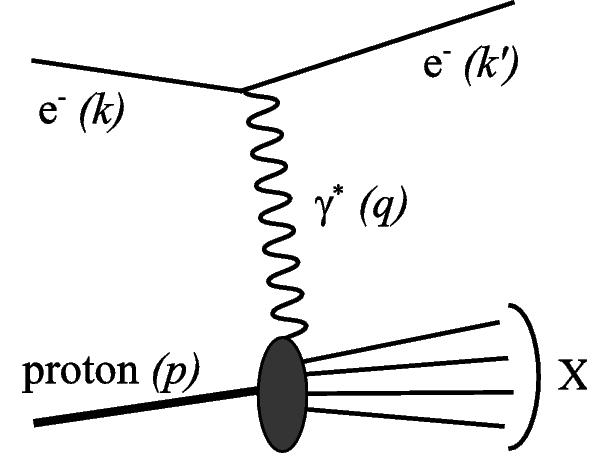
\includegraphics[width=0.6\linewidth]{./figures/deep_inelastic_basic.png}
	\caption{
    A schematic~\cite{Ddn2_2008} of deep inelastic scattering, where the
    incoming electron inelastically scatters off the proton, producing results
    $X$, via virtual photon exchange, $\gamma^*$. The diagram is split into a
    perturbative portion (the electron) and a non-perturbative portion.
    Mathematically, we describe the interaction with kinematic variables
    summarized in Equations~\ref{eq:P}-\ref{eq:x}
  }
	\label{fig:disschematic}
\end{figure}

By the 1970s, collaborations between Bjorken, Feynman, and others had produced
a coherent partonic model which contained quarks and force-mediating gluons.
The concept of Structure functions had been developed. Modified from
Rutherford's original scattering formula, a new formalism to describe the cross
section of deep inelastic scattering incorporated structure functions. Structure
Functions provide a means to separated out the momentum exchange between target
and projectile (via a virtual photon), and isolated this known process from the
total interaction. The $W_1$ and $W_2$, structure functions were defined to be
experimentally measured quantities representing the electron-proton
interaction~\cite{Riordan1992}.

This period of time, from 1970--1990 was truly the golden age of Deep Inelastic
Scattering Experiments. The biggest laboratories responsible for data from this
period were The European Organization for Nuclear Research (CERN), The Stanford
Linear Accelerator Center (SLAC), and The German Electron Synchrotron (DESY).
Thousands of ground-breaking papers were published, such as the CERN's European
Muon Collaboration experiment which showed a measurement of the spin asymmetry
and determination of the proton structure function $g_1$ in muon-proton deep
inelastic scattering \cite{Ashman1988}. 

The formalism of scattering theory continued to evolve during this booming
period.  Though the process of scattering itself has not changed since its
inception in Rutherford's lab, vast improvements in technology have allowed
unprecedented scattering energies with high luminosity accelerators. We now can
take measurements of particles and their properties with exquisite precision.
The level of precision now possible is exemplified in Brookhaven National
Laboratory's E821 Muon ($g$-$2$) experiment--which measured the anomalous
magnetic moment, $g$-$2$, of the muon to a precision of 7 parts in ten
million~\cite{Bennett}.

\clearpage

With the advent of the structure function model, we began an era where matter
ceased to be modeled as a simplistic bound-state of quarks, such as the valence
quark model for the proton, and instead, complex clouds of quark and gluon
interactions. The mathematics of scattering formalism had to change to
accommodate the underlying physical distribution of partonic matter in baryons.
Deep Inelastic Scattering continued to probe various portions of these structure
functions, and the structure of the standard model began to come into focus,
distilled into the relatively simple mathematical structure of group theory. The
standard model is a gauge theory, which contains the internal symmetries of
$SU_{c}(3) \times SU_{L}(2) \times U_{Y}(1)$, Figure~\ref{fig:standardmodel}.
The Standard Model is said by some to be ``complete'' with the discovery of the
Higgs Boson, yet for emergent phenomena such as proton spin, it does not provide
a straightforward prediction. 

\begin{figure}[ht]
	\centering
	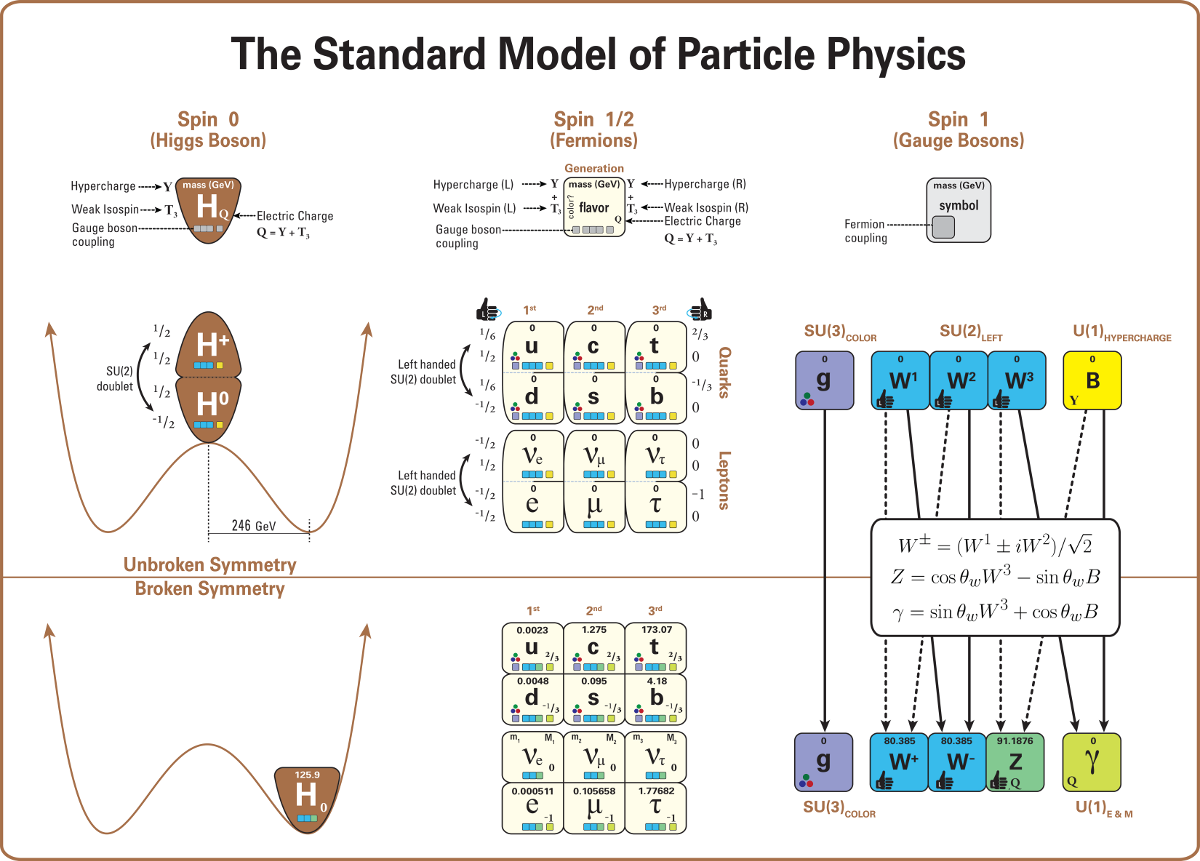
\includegraphics[width=\linewidth]{./figures/standard_model_complete_lowres.png}
	\caption{
		"This diagram displays the structure of the standard model (in a way that
		displays the key relationships and patterns more completely, and less
		misleadingly, than in the more familiar image based on a 4x4 square of
		particles). In particular, this diagram depicts all of the particles in the
		standard model (including their letter names, masses, spins, handedness,
		charges, and interactions with the gauge bosons -- i.e. with the strong and
		electroweak forces). It also depicts the role of the Higgs boson, and the
		structure of electroweak symmetry breaking, indicating how the Higgs vacuum
		expectation value breaks electroweak symmetry, and how the properties of the
		remaining particles change as a consequence."\cite{Boyle2014}.
	}
	\label{fig:standardmodel}
\end{figure}


\clearpage
\section{Modern Deep Inelastic Scattering Experiments}

Here, I hope to highlight the last 40 years or so of physics produced by deep
inelastic scattering experiments. The boundaries of science are pushed by huge
collaborations of men and women working together, starkly contrasting the lonely
pursuits of a handful of scientists in 19th century laboratories.

This era of deep inelastic scattering has unearthed some of the most surprising
and monumental discoveries in physics, from the recent discovery of the
Higgs-particle, to the discovery that protons and neutrons are not fundamental
particles at all, but are instead, highly relativistic balls of gluons.

SLAC Experiments (E80-E155) were some of the first experiments to probe the
proton spin structure, operating from 1978-1999. SLAC pioneered the usage of
spin asymmetries as a means of ruling out models for various parameterizations
of quark structure functions, as well as provided important data constraining
nuclear structure functions. SLAC's experiments focused on understanding the
spin structure of the quarks (but not gluons) within protons.

The European Muon Collaboration at CERN was one of the first major international
efforts to study the underlying structure of protons and neutrons with deep
inelastic scattering. The collaboration produced scientific results from 1979 to
1997. The EMC's major contribution to our understanding of nuclear structure was
to amass evidence which supported the parton model of protons and neutrons, as
well as discovering the self-named `EMC effect', which showed that the volume
`occupied' by quarks scales with heavier nuclei~\cite{Aubert1983}. EMC also
elucidated the effects of quark fragmentation and hadron production, DIS in the
nuclear medium, and produced some of the first measurements of the spin
structure of the proton. Most famously, the EMC originally published the `proton
spin crisis' in its first measurement of the proton spin structure function,
$g1$ where it found the spin carried by the proton's 'valence quarks' is
significantly less than $1/2$~\cite{Ashman1988}. 

CERN produced another collaboration which contributed to our understanding of
nuclear structure, the Spin Muon Collaboration. SMC was active from 1993 to 1998
and used polarized beams of muons to interact with a spin polarized target
(ammonia and later p-butanol). SMC measured virtual photon production
asymmetries, $A_1$, in order to measure information about the proton spin
structure function, $g_1$ (discussed in detail in the following chapter). $g_1$
gives access to the quark polarization of protons. Spin structure physics has
been explored at the COMPASS experiment since 2005. CERN's work to understand
the spin structure of the proton probed the contributions of both the quark, and
gluons. 

The German Electron Synchrotron (DESY) is Germany's the premier accelerator
science laboratory, and has been operating continuously since 1964. DESY's
primary experiments in deep inelastic scattering to understand nuclear structure
have been underway since 1992. DESY operates several deep inelastic scattering
experiments including ZEUS, HERA (H1 and H2) and HERMES.  The scientific goals
of the DESY institute as a whole are broad, since it represents Germany's
premier accelerator physics scientific effort. DESY hosts experiments in
condensed matter physics and astrophysics, addition to its efforts in DIS.
However, the portion of DESY's research program devoted to spin structure seeks
to understand both the quark and gluon contributions to proton spin.

Jefferson Laboratory (JLab) is an electron accelerator complex in Virginia
specializing in the cutting edge of fixed target electron deep inelastic
scattering experiments. Experiments in Hall A, B and C are all involved with
studying both quark and gluon contributions to proton spin.

Finally, there is the Relativistic Heavy Ion Collider, and the experiment
PHENIX. RHIC and PHENIX are discussed in detail in
Chapter~\ref{ch:experimental_apparatus}. This thesis presents an analysis of the
data set recorded in 2013 by the PHENIX detector.

\chapter{Models and Associated Probes For Proton Spin Structure}
\label{ch:modeling_proton_spin}

With the advances made over the last half-century, we have come very close to
obtaining a complete model describing the world around us.  In the realm of
Rapid progress has been made in the last 40 years in the understanding of the
structure of the nucleon. Protons and neutrons make up the majority of the mass
in the visible universe - therefore understanding their nature completely is of
fundamental importance to physics.

In the previous chapter, we discussed in the history behind studying the
structure of matter, leading up to a brief discussion of the contemporary
experiments in proton spin structure. Glaringly, I neglected to discuss the
Relativistic Heavy Ion Collider (RHIC) and the Pioneering High Energy Nuclear
Interaction eXperiment (PHENIX), since I wanted to put the program into a firm
theoretical context in this chapter.

This thesis will discuss the experimental efforts of PHENIX to do something no
other experiment has done - utilize the production of W-Bosons as a direct probe
of proton spin. 

Before we discuss the specifics of this measurement, lets first put proton spin
into a larger context.

\section{Modeling the Proton Structure}

One frequent theme in using particle accelerators to study any kind of nuclear
structure is that we do not ever get to directly look at the innards of a
proton, due to the phenomena of color confinement.

This means that often, we must deal with the process of how partons (quarks,
gluons) fragment and decay after a proton proton collision. Additionally, we
must deal with and account for the scale-variance of the fundamental forces. 

The scale variance of the fundamental forces has large implications for the
strong nuclear force, generally represented by the coupling constant,
$\alpha_S$. This constant scales with distance, and becomes highly
non-perturbative at short distances.

Non perturbative effects are notoriously difficult to include in analytical
models. Additionally, we find that the very structure and distribution of
partons and gluons in the nucleus is a scale-dependent phenomena, that is to
say, if we take measurements at a lower energy, we get a different distribution
of partons and gluons than if we measure at higher energy. This is not to say
that the proton magically changes itself based on energy, but is really more
related to the length scale that we are probing inside of the proton. 

With higher energies, we probe successively shorter length scales. Therefore, to
form a complete picture of proton spin structure, we must probe by scanning over
a broad range of energies (length scales).

Though we generally can analytically deal with writing down models in
perturbative regimes, we cannot simply throw up our hands and give up making
predictions in non-perturbative regimes. To accomplish this, we use a
Factorization Theorem, which provides us a way to mathematically separate an
interaction into perturbative and non-perturbative parts (example,
Figure~\ref{fig:disschematic}). The non-perturbative aspect in the figure (the
X) is often the portion which is experimentally constrained.

\subsection{Structure Functions}

As a note here, for this work on theoretical background of deep inelastic
scattering, I heavily reference Ciprean Gal's clear and coherent introduction to
the subject, published in 2014 (\cite{Gal2014b}), in his thesis describing the
complimentary analysis done at PHENIX at central rapidities.

Given that the proton itself has so far been shown to be a non-perturbative
object, we need a means to model the structure of the interaction when two
protons collide, and generate particles.  Generally, we can calculate a
structure function associated with each hadronic process. The variables we
define to describe the kinematics are (see Figure~\ref{fig:disschematic}):

\begin{gather}
  P \label{eq:P}\\
  Q^2 \equiv -q^2 \label{eq:big_q_sq}\\
    x \equiv { Q^2 \over {2P\cdot q} } \label{eq:x}
\end{gather}

Where $P$  is the total hadron momentum (in our case, the proton's momentum),
$Q^2$ is the energy exchange between the proton and probe lepton, and $x$ is the
fraction of the total proton's momentum carried by the quark scattering with the
lepton. $q$, in Equation~\ref{eq:x} is four-momentum transferred from the lepton
to the quark. 

We can then write down structure functions in terms of these variables. We have:

\begin{gather}
  F_1(x,Q^2) = {1 \over 2}\sum_f e_f^2 \left(q_f(x)+\bar{q}(x)\right)
  \label{eq:f1} \\
  F_2(x,Q^2) = 2xF_1(x,Q^2)\label{eq:f2}
\end{gather}

The subscript, $f$ refers to the quark flavors represented in the structure
functions, with $e_f$ referring to the charge of each quark being summed over
(i.e. ${\pm}{1\over3}$ or ${\pm}{2\over3}$). $q(x)$ refers to the parton
distribution function associated with each quark flavor. 

An integration over the momentum fraction, $x$ of Equation~\ref{eq:f2} and the
gluon structure function $g(x)$ yields the familiar 'valence quark' structure of
the proton, i.e. two up-quarks and one down quark, with remaining quark flavors
$q_h$ summing to zero:

\begin{gather}
	\int_0^1 F_2(x,Q^2) + g(x) dx 
	= \int_0^1 
	\left(
		x\sum_f e_f^2 \left(q_f(x)+\bar{q}(x)\right) 
	\right) 
	+ g(x) dx \label{eq:f2_int_1} \\
	\int_0^1 \left(u(x)+\bar{u}(x) dx \right) dx = 2  \label{eq:up_quark_valence} \\
	\int_0^1 \left(d(x)+\bar{d}(x) dx \right) dx = 1  \label{eq:down_quark_valence} \\
	\int_0^1 \left(q_h(x)+\bar{q}_h(x) dx \right) dx = 0 \label{eq:other_quark_valence}
\end{gather}

The rest of the world data on $F_2(x,Q^2)$ is summarized in
Figure~\ref{fig:f2_world_data}

\begin{figure}
  \centering
  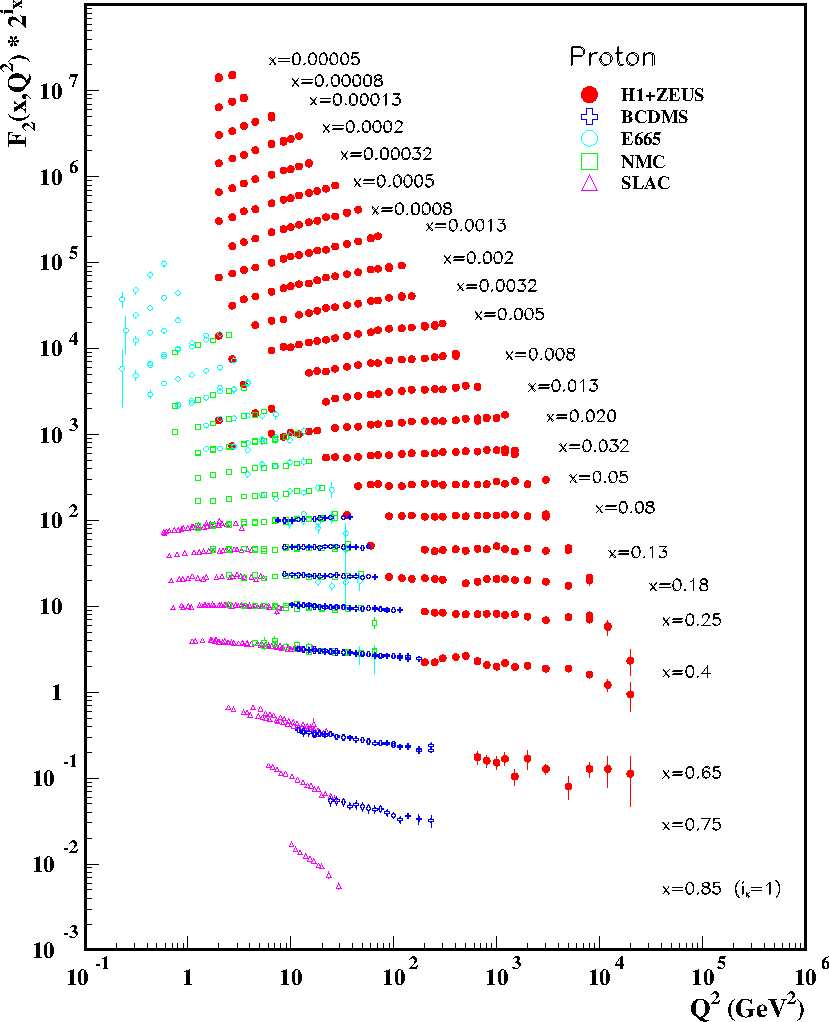
\includegraphics[width=\linewidth]{./figures/F2_structure_function.pdf}
  \caption{
		Here, we see "the proton structure function, $F_2^p$ measured in
		electromagnetic scattering experiments of electrons and positrons on
		protons" from experiments including H1+Zeus, BCDMS, E665, NMC and
		SLAC~\cite{ReviewEidelman2012}
  }
  \label{fig:f2_world_data}
\end{figure}

From this dataset, we can extract Parton Distribution Functions for any
combination of $x$ and $Q^2$. Under this particular framework, we can use the
DGLAP evolution equations to evolve PDFs observed at one $Q^2$ to some other
$Q^2$~\cite{Altarelli2009}. One particular advantage of hadron colliers is to
measure the interactions between gluons and partons between two colliding
partons. 

\section{Parton Distribution Functions}

\begin{figure}[ht]
  \centering
  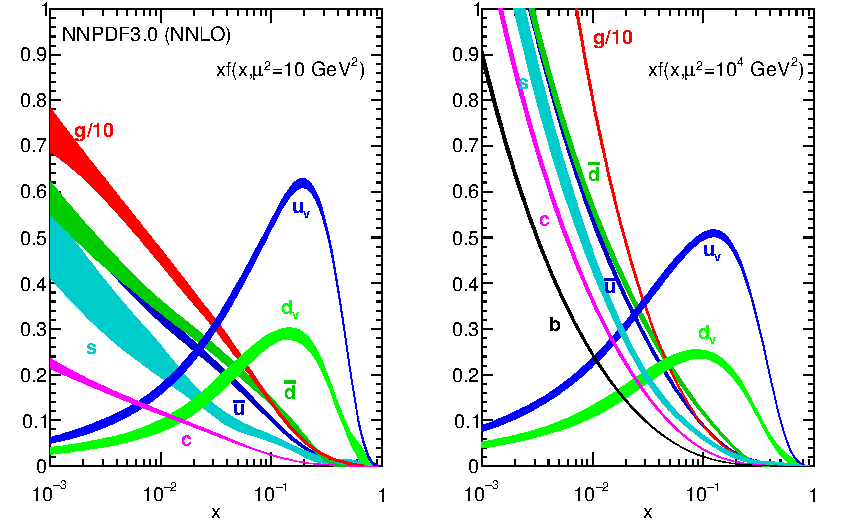
\includegraphics[width=0.7\linewidth]{./figures/unpolarized_pdfs.pdf}
  \caption{
    stuff~\cite{ReviewEidelman2012}
  } 
  \label{fig:unpolarized_pdf}
\end{figure}

\section{Polarized Parton Distribution Functions}
\label{sec:polarized_pdfs}

\begin{figure}
  \centering
  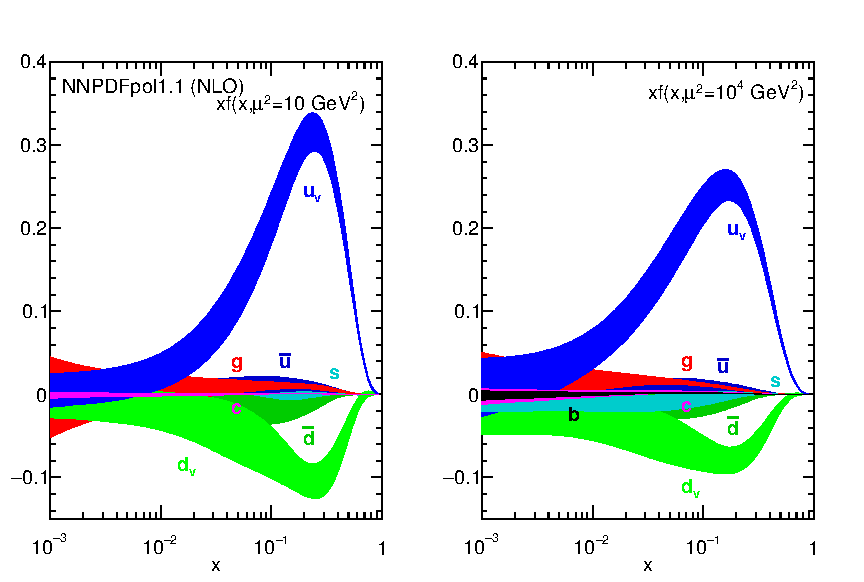
\includegraphics[width=0.7\linewidth]{./figures/polarized_pdfs.pdf}
  \caption{
    stuff~\cite{ReviewEidelman2012}
  }
  \label{fig:polarized_pdfs}
\end{figure}

Discuss DSSV fits
\begin{figure}
  \centering
  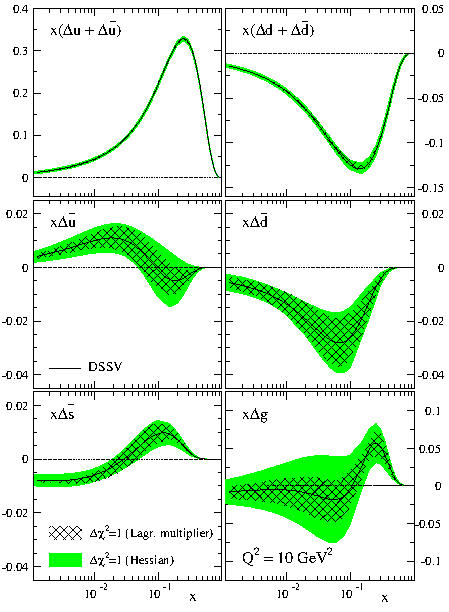
\includegraphics[width=\linewidth]{./figures/polarized_pdfs_dssv.pdf}
  \caption{
    stuff    
  }
  \label{fig:dssv_pdfs}
\end{figure}

\section{Proton Spin Decomposition with the Ellis-Jeffe Sum Rule }

{\noindent}Gauge invariant Ellis-Jeffe
\begin{equation}
  \braket{P,{1\over2}|\hat{J_z}|P,{1\over2}}  
 = {1\over2} = {{1\over2}\Delta \Sigma +L_q+J_g}
\label{eq:ellis_jeffe_sum}
\end{equation}

{\noindent}Infinite momentum decomposition:
\begin{equation}
  \braket{P,{1\over2}|\hat{J_z}|P,{1\over2}}  
  = {1\over2} = {{1\over2}\Delta \Sigma +L_q+\Delta g + L_g}
  \label{eq:infmom_ellis_jeffe_sum}
\end{equation}

{\noindent}Quark decomposition:
\begin{equation}
  {\Delta \Sigma} =
  {
    (\Delta u+\Delta \bar{u})
    +(\Delta d + \Delta \bar{d})
    +(\Delta s + \Delta \bar{s})
  }
  \label{eq:quark_spin_decomposition}
\end{equation}

\section{The Spin Asymmetry: An Experimental Probe }
Write in terms of the cross-section of polarized scattering.

\begin{figure}[ht]
  \centering
  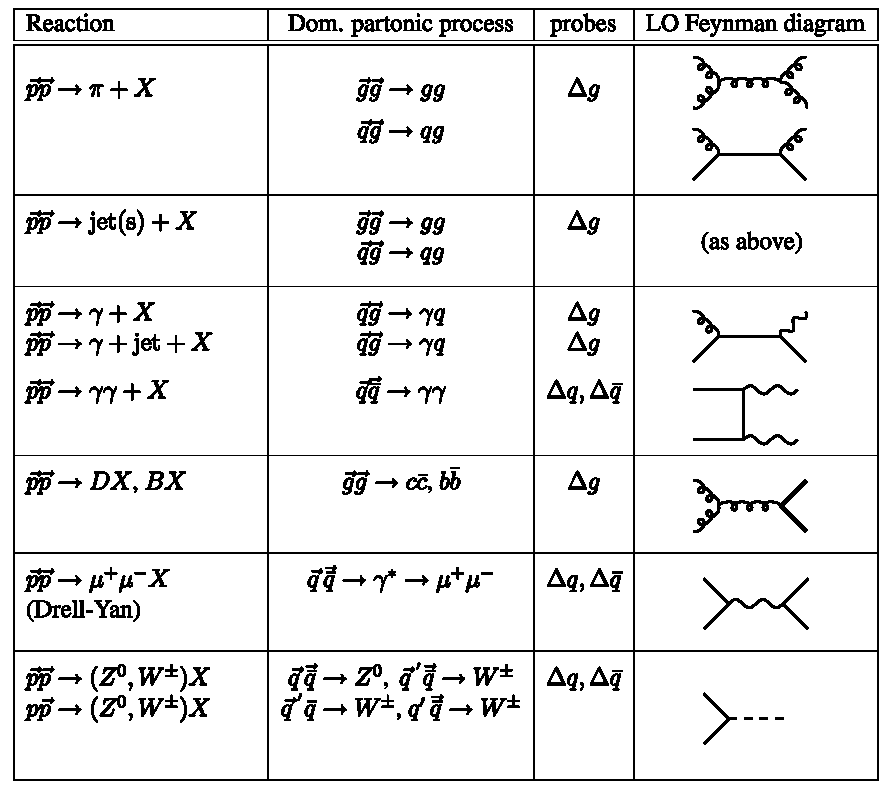
\includegraphics[width=\linewidth]{./figures/spin_probes.pdf}
  \caption{
    A summary of the various probes for longitudinally polarized protons. The
    \textbf{"Reaction"} column summarizes the reaction observed experimentally.
    The \textbf{"Dom. partonic process"} column describes the dominant process
    at the partonic level. The \textbf{"probes"} column shows which proton spin
    structure can be measured with the reaction. Finally, the leading order
    Feynman diagram for the partonic process is drawn. Figure is reproduced
    from: \cite{Aidala2005}.
  }
  \label{fig:spin_probes_masterspin}

\end{figure}

\section{W Production}


Though W-Bosons obviously can be created in collisions with the right
ingredients and correct energy, the W-Bosons that we're interested in at RHIC
are very special. The collision conditions around the protons at colliding at
PHENIX provides just enough energy to create real W-Bosons from interaction of
quarks and anti-quarks between two colliding protons. The energy is not
sufficiently high enough to produce real W-Bosons from other processes in
amounts which would significantly dilute the primary source.

The standard model tells us that W production occurs through a pure vector-axial
interaction, this implies that the helicity of the parents particles - in
particular $u+\bar{d}\rightarrow W^+$ and $\bar{u}+d\rightarrow W^-$ have fixed
helicities, due to the relativistic final state neutrino (which is not measured,
of course). To visualize the leading order of W production, with regards to the
quark-sea element being probed, the leading order diagrams for the interaction
are shown in Figure~\ref{fig:w_probe_leading_order}~\cite{Aidala2005}

Since $\Delta q$, the polarized parton distribution function can be split into
contributions from valence quarks, and also sea quarks, understanding $\Delta
\bar{q}$ is an important step towards understanding $\Delta q$ better to better
understand the total proton spin.

\begin{figure}[ht]
  \centering
  \begin{subfigure}[b]{\textwidth}
    \centering
    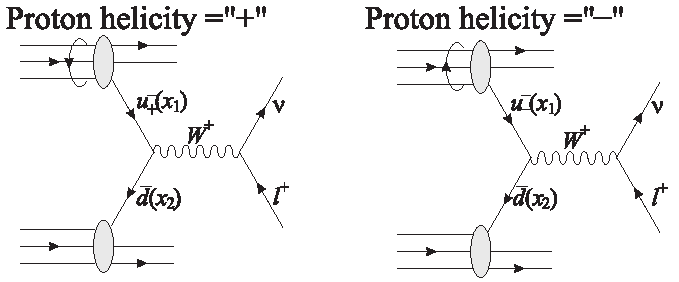
\includegraphics[width=0.8\linewidth]{./figures/w_plus_u_probe.pdf}
    \caption{
      Probe for $\Delta u$ at lowest order.
    }
    \label{fig:u_probe}
  \end{subfigure}
  \begin{subfigure}[t]{\textwidth}
    \centering
    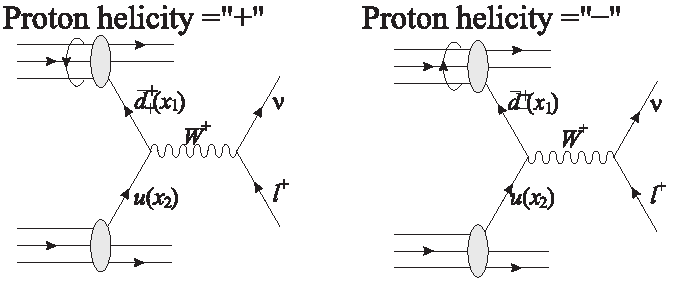
\includegraphics[width=0.8\linewidth]{./figures/w_plus_dbar_probe.pdf}
    \caption{
      Probe for $\Delta\bar{d}$ at lowest order
    }
    \label{fig:dbar_probe}
  \end{subfigure}
  \caption{
    Real $W^+$ production as produced at PHENIX. The helicity of the initial
    state fixes the helicity of the partonic participants due to the
    relativistic final state of the neutrino + the handedness of the W boson.
    $x_1$ and $x_2$ are the momentum fractions of the quarks participating from
    the participant partons~\cite{Aidala2005}. 
  }
  \label{fig:w_probe_leading_order}
\end{figure}

Though both protons in the collision are polarized, the polarization of one
participant proton can be effectively ignored by summing over all polarization
states for one of the two protons. With this assumption, we may construct a
single spin asymmetry for colliding protons by counting difference in the number
of positively and negatively polarized W's produced in collisions, scaled by the
total production:

\begin{equation}
  {{A_L}^W} =
  {{{1}\over{P}}\times{{N_{-}(W)-N_{+}(W)}\over{{N_{-}(W)+N_{+}(W)}}} }
  \label{eq:w_production_asymmetry}
\end{equation}

This is a relatively easy experimental probe to measure (assuming that we can
accurately count events which produced a W, which naturally, is nearly
impossible, as we will see in Section~\ref{sec:sbr}).

As we saw earlier, in Section~\ref{sec:polarized_pdfs}, we can write an
asymmetry in terms of the scattering cross section for the process responsible
for particle yields. These cross-sections were shown to be written in terms of
polarized parton distribution functions, thus, we cut to the chase to write down
the full expression of the theoretical asymmetries for this process in terms of
those parton distribution functions.

The following equations all contain an implied integration over $x_1$ and $x_2$.

For $W^+$ and $u$:
\begin{equation}
  {A_L^{W^+}} = 
  {
    {u_-^-(x_1)\bar{d}(x_2)-u_+^-(x_1)\bar{d}(x_2)}
    \over
    {u_-^-(x_1)\bar{d}(x_2)-u_+^-(x_1)\bar{d}(x_2)}
  }  
  \label{eq:al_u_full}
\end{equation}

For $W^+$ and $\bar{d}$
\begin{equation}
  {A_L^{W^+}} = 
  {
    {\bar{d}_-^+(x_1)u(x_2)-\bar{d}_+^+(x_1)u(x_2)}
    \over
    {\bar{d}_-^+(x_1)u(x_2)+\bar{d}_+^+(x_1)u(x_2)}
  }  
  \label{eq:al_dbar_full}
\end{equation}

Observationally, we see a superposition of \ref{eq:al_u_full} and
\ref{eq:al_dbar_full}, which is expressed in
Equation~\ref{eq:al_superposition_pos}:

\begin{equation}
  {A_L^{W^+}} = 
  {
    {
      \Delta u(x_1)\bar{d}(x_2)-\Delta \bar{d}(x_1)u(x_2)
    }
    \over
    {
      u(x_1)\bar d(x_2)+\bar(d)(x_1)u(x_2)
    }
  }
  \label{eq:al_superposition_pos}
\end{equation}

For the case of $W^-$, we observe $\bar{d}$ and $u$:
For $W^-$ and $d$:
\begin{equation}
  {A_L^{W^+}} = 
  {
    {d_-^-(x_1)\bar{u}(x_2)-d_+^-(x_1)\bar{u}(x_2)}
    \over
    {d_-^-(x_1)\bar{u}(x_2)-d_+^-(x_1)\bar{u}(x_2)}
  }  
  \label{eq:al_d_full}
\end{equation}

For $W^-$ and $\bar{u}$
\begin{equation}
  {A_L^{W^+}} = 
  {
    {\bar{u}_-^+(x_1)d(x_2)-\bar{u}_+^+(x_1)d(x_2)}
    \over
    {\bar{u}_-^+(x_1)d(x_2)+\bar{u}_+^+(x_1)d(x_2)}
  }  
  \label{eq:al_ubar_full}
\end{equation}

Observationally, we see a superposition of \ref{eq:al_d_full} and
\ref{eq:al_ubar_full}, which is expressed in
Equation~\ref{eq:al_superposition_neg}:

\begin{equation}
  {A_L^{W^-}} = 
  {
    {
      \Delta d(x_1)\bar{u}(x_2)-\Delta \bar{u}(x_1)d(x_2)
    }
    \over
    {
      d(x_1)\bar u(x_2)+\bar(u)(x_1)d(x_2)
    }
  }
  \label{eq:al_superposition_neg}
\end{equation}

Kinematics of the collision can simplify the equations even further, when at
very forward or very backward rapidities~\cite{Aidala2005}. Concretely, this is
shown via integration over the momentum fractions, $x_1$ and $x_2$, explicitly
writing the W decay in terms of the scattering cross section for polarized
proton collisions (a derivation reproduced from Hideyuki Oide's
thesis~\cite{Oide2012}):

\begin{multline}
  {
    d\sigma
    \left(
      p^{\Rightarrow}+p\rightarrow W^+\rightarrow \ell+\nu_{\ell}
    \right)
  } 
  = \\
  {
    {K\over3}\int dx_1dx_2\sum_{i,j}
    \left(
    q_{i-}^\Rightarrow(x_1)\bar{q}_{j+}(x_2) +
    \bar{q}_{j+}^\Rightarrow(x_1)q_{i-}(x_2)
    \right)
  }  \\
  \times
  {
    d\hat{\sigma}(q_i+\bar{q}_j\rightarrow W^+\rightarrow \ell^+ + \nu_{\ell})
  }
\end{multline}

{\noindent}Similarly, we may write the interaction cross-section for the
opposite helicity in the initial state:

\begin{multline}
  {
    d\sigma
    \left(
      p^{\Leftarrow}+p\rightarrow W^+\rightarrow \ell+\nu_{\ell}
    \right)
  } 
  = \\
  {
    {K\over3}\int dx_1dx_2\sum_{i,j}
    \left(
    q_{i-}^\Leftarrow(x_1)\bar{q}_{j+}(x_2) +
    \bar{q}_{j+}^\Leftarrow(x_1)q_{i-}(x_2)
    \right)
  }  \\
  \times
  {
    d\hat{\sigma}(q_i+\bar{q}_j\rightarrow W^+\rightarrow \ell^+ + \nu_{\ell})
  }
\end{multline}

Neglecting quark mass, we can assume that the helicity state of the quarks is
identical to the chirality state. Then, we substitute in the definition for
polarized parton distribution functions $\Delta q \equiv q_{+}^{\Rightarrow} -
q_{-}^{\Rightarrow}$, and sum over quark flavors, neglecting strange
contributions:

\begin{align}\label{eq:al_theory_quarks}
  {
    A_L
    \left(
      p^{\Rightarrow}+p\rightarrow W^+ \rightarrow \ell^+ +\nu_{\ell}
    \right)
  } &=  
  {
    {
      \int dx_1 dx_2 \sum_{i,j}
      \left(
        -\Delta q_i(x_1)\bar{q}_j(x_2)
        +\Delta \bar{q}_j(x_1)q_i(x_2)
      \right)\cdot d \hat{\sigma}
    }
    \over
    {
      \int dx_1 dx_2
      \sum_{i,j}(q_i(x_1)\bar{q}_j(x_2)+\bar{q}_j(x_1)q_i(x_2))\cdot d\hat{\sigma}
    }
 }\\
 & \approx  \nonumber
 {
   {
      \int dx_1 dx_2 
      \left(
        -\Delta u(x_1)\bar{d}(x_2)
        +\Delta \bar{d}(x_1)u(x_2)
      \right)\cdot d \hat{\sigma}
   }
   \over
   {
      \int dx_1 dx_2 (u(x_1)\bar{d}(x_2)+\bar{d}_j(x_1)u(x_2))\cdot d\hat{\sigma}
   }
 }
\end{align}

Since we have restricted ourselves to only the case for $u\bar{d}$, we are of
course looking at the case of $A_L^{W+}$. We may rewrite
Equation~\ref{eq:al_theory_quarks} to reflect its rapidity dependance:

\begin{equation}
  {A_L^{W+}(y_{\ell})} = 
  {
    {
     \int dx_1 dx_2 
     \left(
       -\Delta u(x_1)\bar{d}(x_2)(1-cos\hat{\theta})^2
       +\Delta \bar{d}(x_1)u(x_2)(1+cos\hat{\theta})^2
     \right)
    }
    \over
    {
       \int dx_1 dx_2 
       \left(
       (u(x_1)\bar{d}(x_2)   (1-cos\hat{\theta})^2
      +\bar{d}_j(x_1)u(x_2)) (1+cos\hat{\theta})^2
        \right)
    }
  }
  \label{eq:al_w_pos_rapidity_dependance}
\end{equation}

In this case, we follow Dr. Oide's convention of redefining $\hat{\theta}$ in
terms of the angle between the direcion of momentum of the polarized proton and
the leptop in the center of mass frame. Therefore we see kinematic isolation of
the polarized pdfs at forward or backward rapdity.\\

{\noindent}We may write $A_L^{W-}(y_{\ell})$ similarly:

\begin{equation}
  {A_L^{W-}(y_{\ell})} = 
  {
    {
     \int dx_1 dx_2 
     \left(
       -\Delta \bar{u}(x_1)d(x_2)(1-cos\hat{\theta})^2
       +\Delta d(x_1)\bar{u}(x_2)(1+cos\hat{\theta})^2
     \right)
    }
    \over
    {
       \int dx_1 dx_2 
       \left(
         (\bar{u}(x_1)d(x_2)   (1-cos\hat{\theta})^2
         +d_j(x_1)\bar{u}(x_2)) (1+cos\hat{\theta})^2
        \right)
    }
  }
  \label{eq:al_w_neg_rapidity_dependance}
\end{equation}
\clearpage
\section{Cross Sections and Luminosity}
\begin{itemize}
		\item vernier analysis note intro, equations
		\item summarize the papers on Lumoninosity
\end{itemize}

\textbf{Questions I'd Like to Answer in this Chapter}
\begin{enumerate}
    \item Why can we collide two polarized protons, but pretend that only one of
      them is polarized? What if summing over polarization states doesn't
      'cancel' this out?
    \item Why is $A_L$ an appropriate probe for proton spin
    \item How exactly do we go from a measurement of $A_L$ to an understanding
      of proton spin?
    \item Why do we need to calculate $A_{LL}$? What does it tell us? Why do we
      combine the helicities in the way we do, to define $A_{LL}$?
\end{enumerate}

Double spin asymmetry:

\begin{equation}
  A_{LL} = {
    {d\sigma^{\Rightarrow\Rightarrow}-d\sigma^{\Leftarrow\Rightarrow}}
    \over
    {d\sigma^{\Rightarrow\Rightarrow}+d\sigma^{\Leftarrow\Rightarrow}}
  }
\end{equation}
\clearpage

\chapter{The Relativistic Heavy Ion Collider}

\section{Overview}
While there have been many experiments which have performed deep inelastic
scattering over the years, the experiments built around the Relativistic Heavy
Ion Collider at Brookhaven National Laboratory are positioned to take advantage
of this unique accelerator. 

\begin{figure}[ht]
  \centering
  \begin{subfigure}[b]{\textwidth}
    \centering
    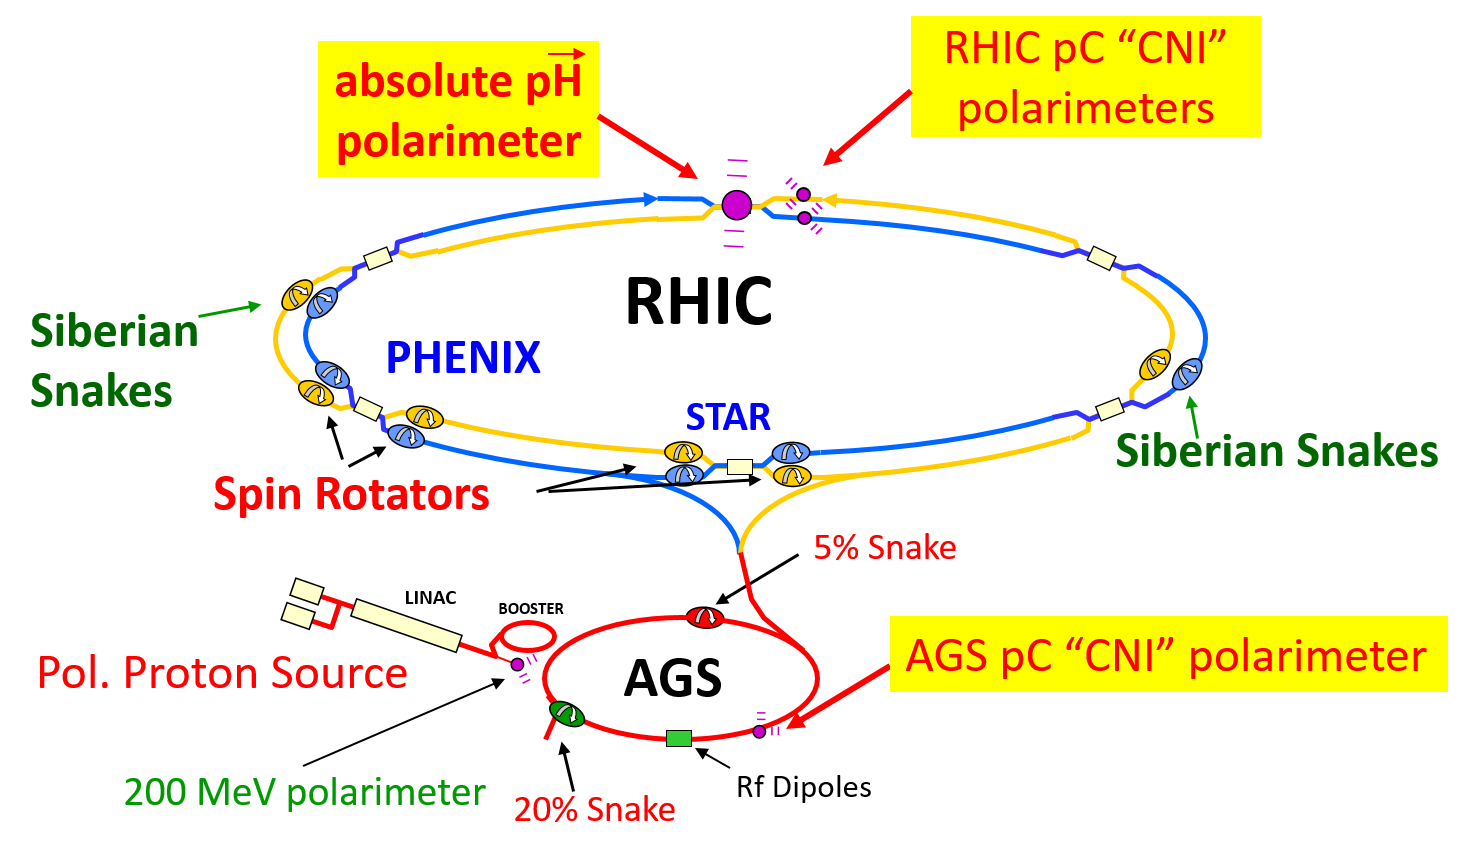
\includegraphics[width=0.8\linewidth]{./figures/kiyoshi_tanida_rhic_schematic.png}
    \caption{Diagram of RHIC Accelerator Complex, (Figure from Kiyoshi Tanida)}
    \label{fig:rhic_schematic} 
  \end{subfigure}
  \begin{subfigure}[b]{\textwidth}
    \centering
    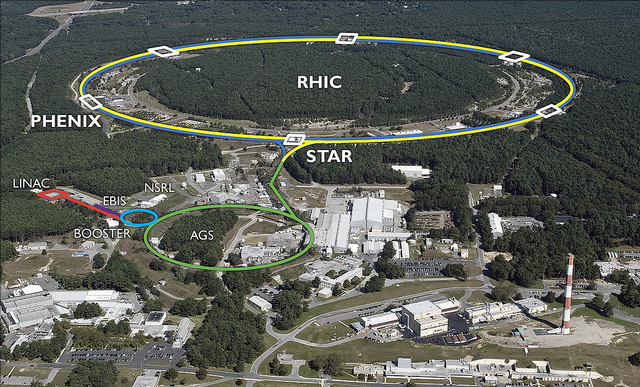
\includegraphics[width=0.8\linewidth]{./figures/7979381212_fddf3f1ab4_z.jpg}
    \caption{Aerial photograph of RHIC Complex \cite{BNLFlickr2011}}
    \label{fig:rhic_aerial}
  \end{subfigure}
  \caption{
		A diagram of the acceleration process of RHIC is shown in the top panel, and
		aerial view is shown in thin the bottom panel. RHIC is nearly four miles in
		circumference and collides a variety of ions at center-of-mass energies
		between $5$ Gev $\sqrt{s}$  and $510$ GeV $\sqrt{s}$.
  }
  \label{fig:rhic_complex}
\end{figure}

The Relativistic Heavy Ion Collider (RHIC) is the world's only intersecting ring
particle accelerator which is capable of colliding polarized proton beams. The
beams are differentiated with the mnemonic ``Blue'' and ``Yellow'' labels. The
blue beam circulates clockwise when viewed from above the RHIC complex, the
yellow beam circulates counter-clockwise. As is typical for intersecting ring
experiments, the beams are bunched, with bunches of ions intersecting at
designated intersection points, around which experiments are built.  The filled
bunches from the blue and yellow beams cross at a frequency of 106 nanoseconds.
PHENIX's timing is set to correspond to the crossing rate of the blue and yellow
beams. Because bunches always collide simultaneously, the blue beam timing clock
is used as a matter of convention, though there are other timing clocks
available for use. The bunches in the beams are numbered as a means of
associating the bunch polarization configuration with the bunch crossing at each
interaction region. This is necessary for any measurement which requires a
knowledge of the initial polarization state of colliding hadrons (such as any
spin physics measurement). This will be discussed more in the section of
discussing the beam polarization at RHIC~\ref{sec:beam_polarization}.

RHIC generally separates data taking into beam `fills' which are uniquely
numbered, and for which general data characterizing the machine state is logged
in various databases and online logbooks. Logging is an important part of data
quality assurance, but also plays a fundamental role in the physics. For
example, the initial spin state of the colliding bunches is logged in databases,
without which, spin analyses are impossible. The trigger configuration is
recorded along with the rates associated with each trigger. Data logged into
logbooks and databases characterizing a fill's performance also plays an
important forensic role with regards to solving issues which occurred during
data taking, but were not immediately caught. Furthermore, because PHENIX is an
international collaboration, this logged data is fundamentally important to
communicating the state of the machine and data collection to the collaboration,
as well as establishing a record of operations.  

RHIC fills are composed of a unique population of bunched ions, circulating
around the rings. During polarized fills, every bunch is polarized according to
a planned polarization pattern. At the end of each fill, (typically 8 hours of
collisions), the beam is dumped, and a new fill is generated.  Experiments built
around RHIC generally subdivide fills into `runs', where a run is a period of
time where the experiment is taking data during which there were no obvious
machine malfunctions. When major issues occur during a run, data taking is
interrupted until the problem is remedied, and the data is discarded. At PHENIX,
runs are always segregated within a fill--no run will ever contain data from
multiple fills, due to the additional complexity of potentially changing machine
conditions, significant down-time between fills, and the potential of beam-dumps
into sensitive high voltage enabled electronics.

Scientists at RHIC have come up with many ingenious ways to create and maintain
beam polarization (Section~\ref{sec:beam_polarization}), once this is
accomplished, various kinematically select probes are engineered, based on
collisions observed which provide important cross-checks to DIS data as well as
original discoveries and measurements of proton structure. RHIC is a unique
collider in that it is quite flexible. Beams may be transversely or
longitudinally polarized, a variety of ions may be used to fill the beams. To
date, RHIC has collided many beam ions and species, summarized in
Figure~\ref{fig:rhic_early_run_summary} and
Figure~\ref{fig:rhic_late_run_summary}.

RHIC is an facility which has been built on top of previous accelerator
experiments--a Linear Accelerator, a booster ring, and an Alternating Gradient
Synchrotron, all of which now have been re-purposed to create the necessary beam
injection conditions appropriate for RHIC. Many experiments are still set up
around various egress points along the acceleration chain, which are publicised
on the Brookhaven National Laboratory website \url{www.bnl.gov}

\begin{figure}[ht]
  \centering
  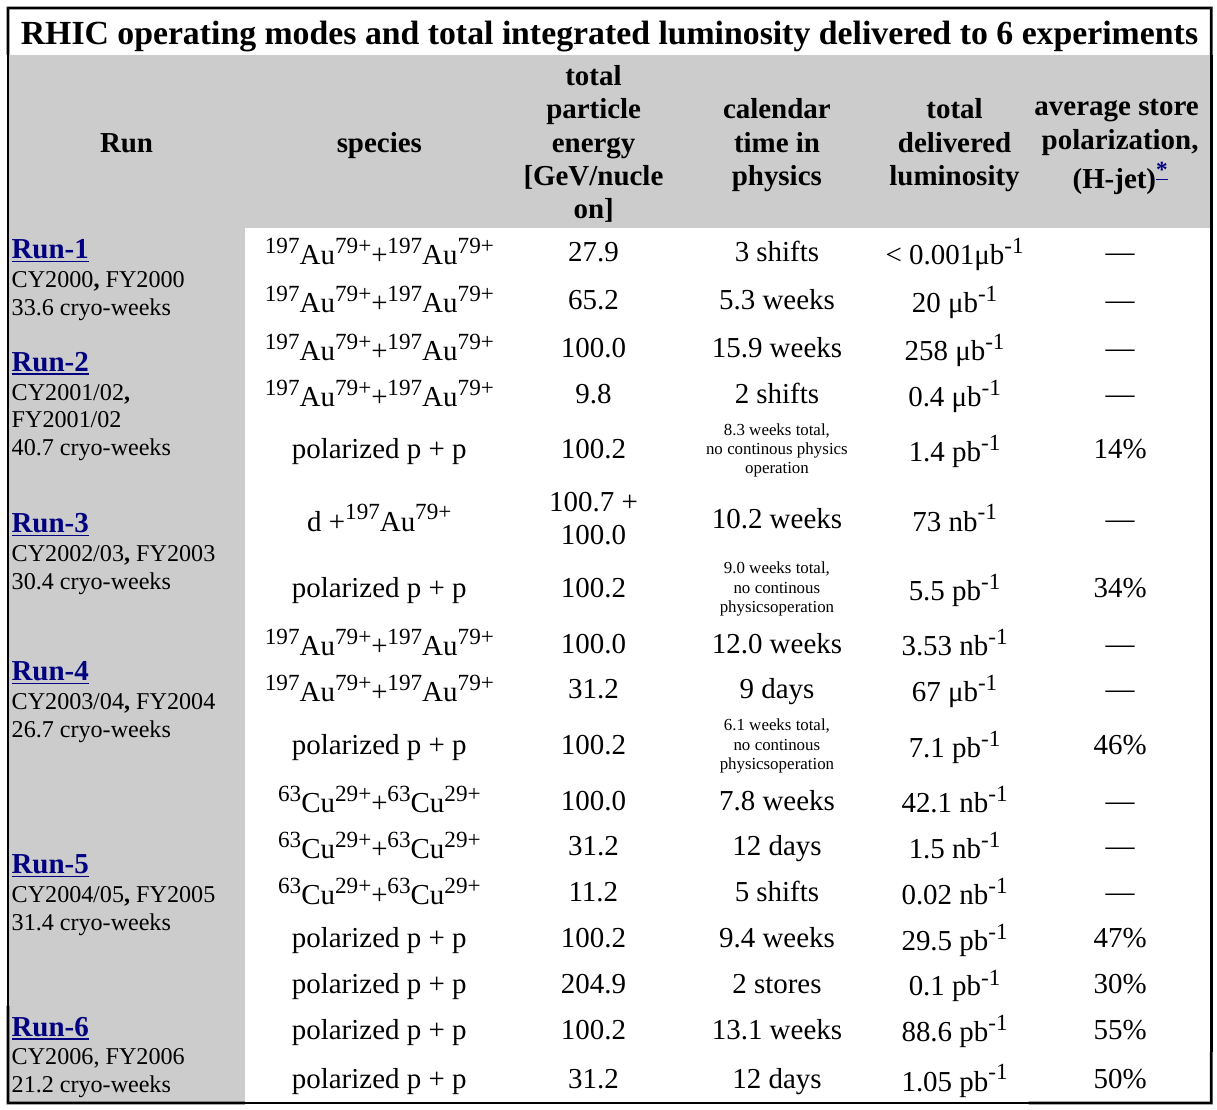
\includegraphics[width=0.8\linewidth]{./figures/rhic_early_run_summary.png}
  \caption{ 
    Runs 1--3 at RHIC focused on commissioning work for experiments measuring
    collisions at RHIC. Work was mostly characterized by heavy-ion measurements
    related to understanding Quark-Gluon Plasma. The spin program began with Run
    5. Table produced from data posted at the RHIC run page \cite{Fischer2016}.
  }
  \label{fig:rhic_early_run_summary}
\end{figure}

\begin{figure}[ht]
  \centering
  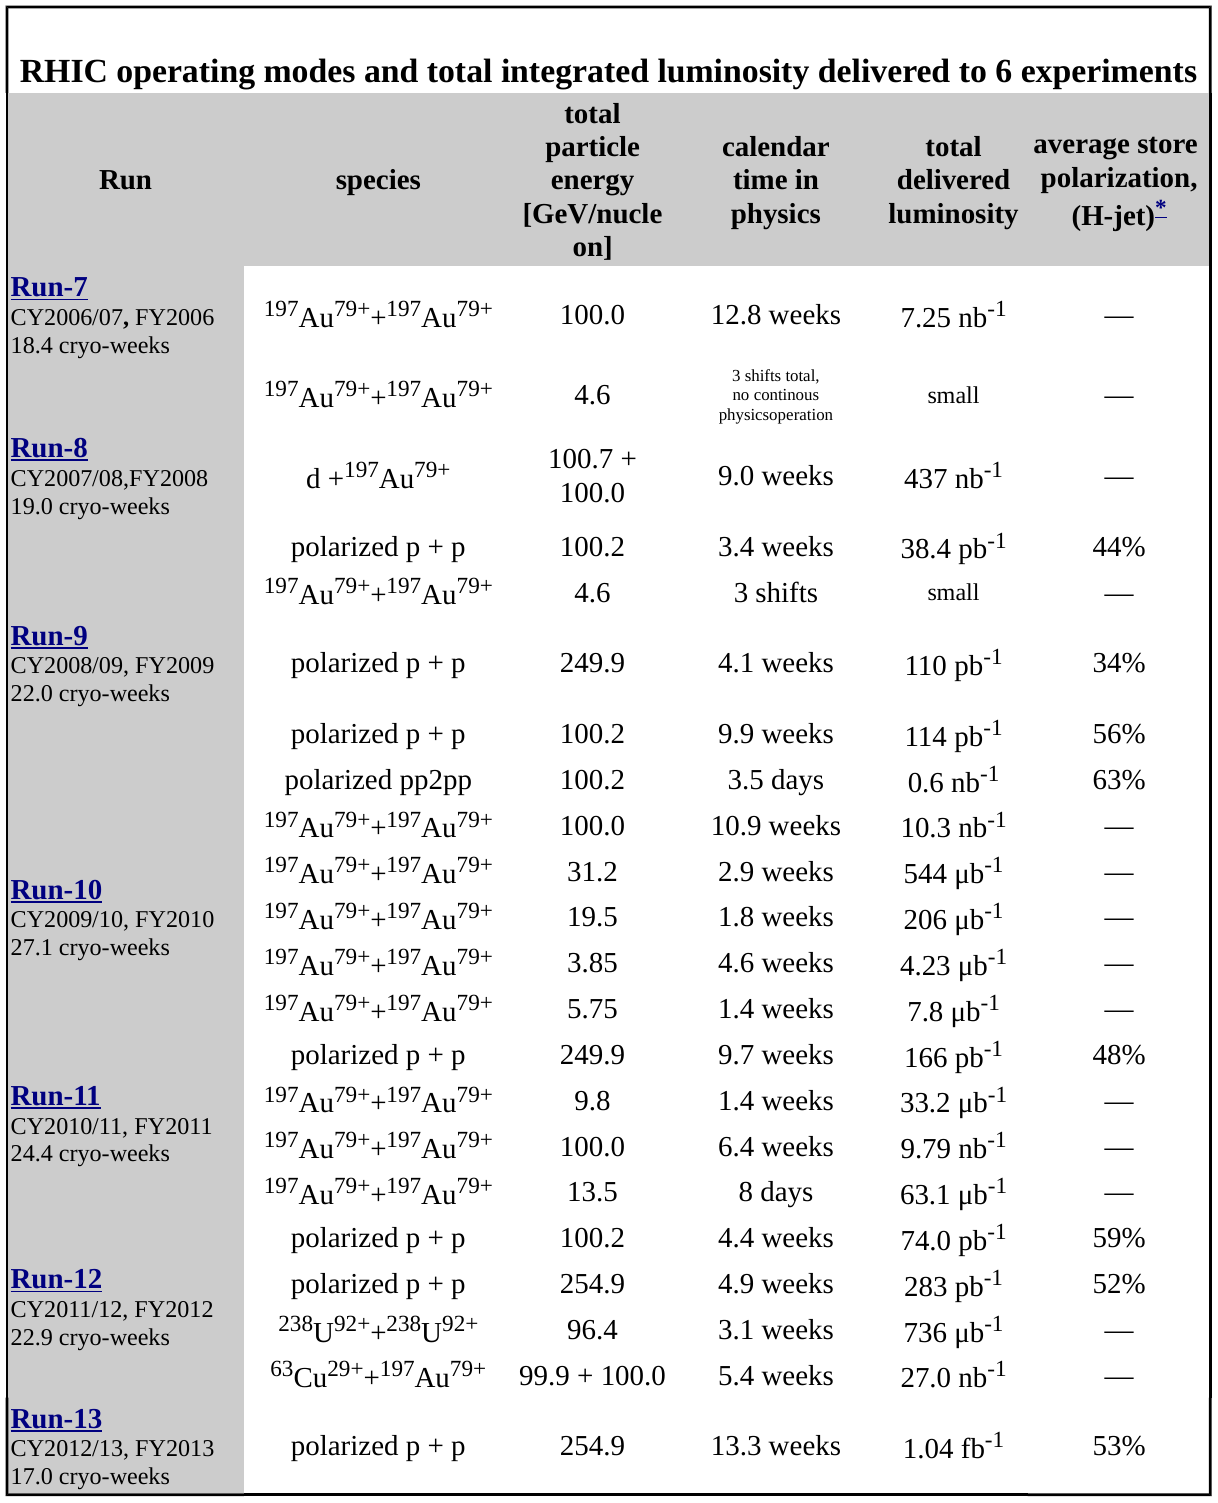
\includegraphics[width=0.8\linewidth]{./figures/rhic_late_run_summary.png}
  \caption{ 
    Though RHIC is currently still running (as of May 9, 2016), I include runs
    here up to and including the run producing my data set (Run 13). An
    unprecedented 13.3 cryo-weeks of running was awarded to the W-Physics
    group.  Table produced from data posted at the RHIC run
    page \cite{Fischer2016}.
  }
  \label{fig:rhic_late_run_summary}
\end{figure}

At the time of writing of this Thesis (Spring of 2016), there are two
experiments which are actively taking data from collisions produced by RHIC: The
Pioneering High Energy Nuclear Interaction Experiment (PHENIX,
Section~\ref{sec:PHENIX}, Figure~\ref{fig:phenix_and_star}), and the Solenoidal
Tracker at RHIC (STAR, Figure~\ref{fig:phenix_and_star}). STAR and PHENIX are
complimentary to each other--PHENIX has a very high precision centrally covering
Electromagnetic Calorimeter, and other high precision detectors, but lacks full
kinematic coverage, whereas STAR has lower precision (with some measurement
dependent exceptions), but has the advantage of nearly full kinematic coverage
around the beam intersection at its center.

RHIC's luminosity and beam polarization has been continuously improving
(Figure~\ref{fig:rhic_luminosity}) since RHIC was first turned on. As we will
discuss later (Section~\ref{sec:forward_upgrade}), the increased luminosity
observed in 2013, was maximally leveraged with upgrades to the PHENIX detector.

\begin{figure}[ht]
  \centering
  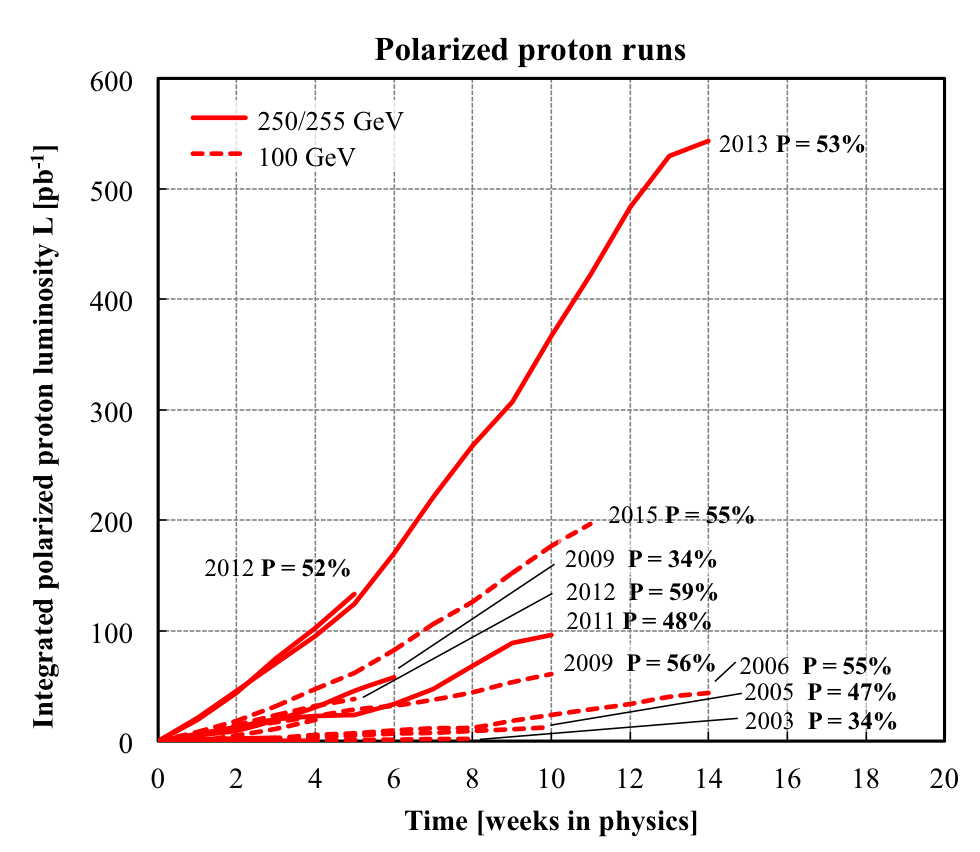
\includegraphics[width=0.8\linewidth]{./figures/RhicLuminosityPP.png}
  \caption{
    Upgrades to RHIC's electron lens have enabled massive improvements to
    luminosity--seen in the year 2013. The high luminosity was taken advantage
    of with an extra long proton+proton run. Figure obtained from
     \cite{Fischer2016}
  }
  \label{fig:rhic_luminosity}
\end{figure}


\clearpage

\subsection{Experimental Apparatus}

\begin{figure}[ht]
  \centering
  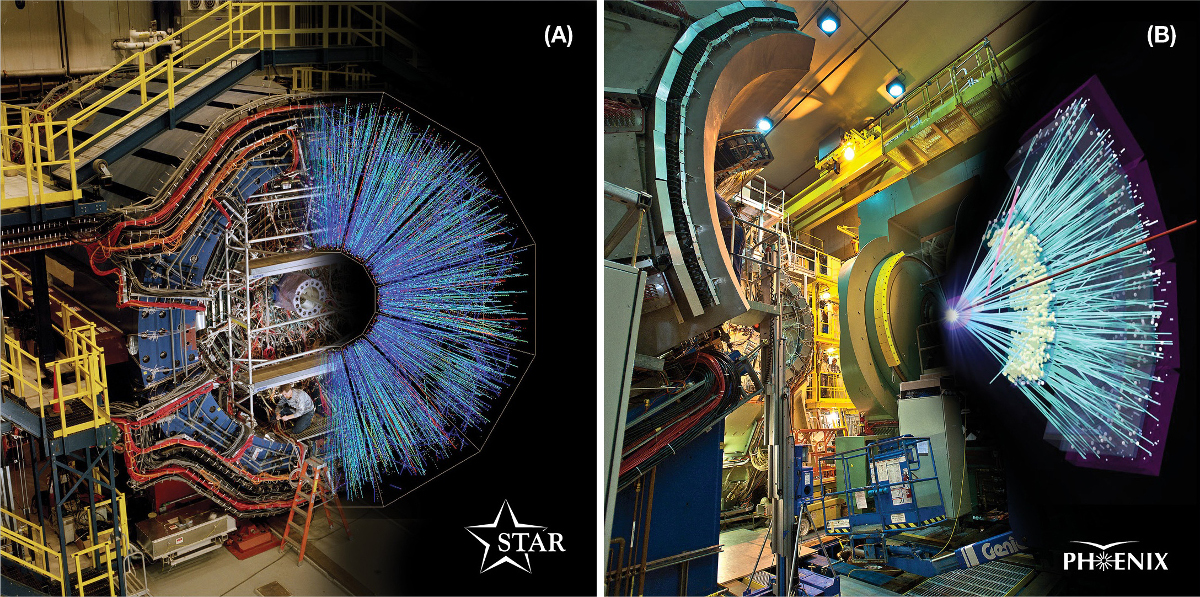
\includegraphics[width=\linewidth]{./figures/rhic_graphics_fig2-hr.jpg}
  \caption{
    STAR (a) and PHENIX (b) with cutaways showing the event display for a
    heavy-ion collision as reconstructed by the detectors' electromagnetic
    calorimeters~\cite{Walsh2012}.
  }
  \label{fig:phenix_and_star}
\end{figure}

RHIC accelerates ions in a multi-stage process, summarized in
Figure~\ref{fig:rhic_complex}. The source of the beams is the \textbf{Electron
Beam Ion Source}, built on top of a $200$ MeV linear accelerator (Linac). Once
ions are injected into the Linac, they travel to the \textbf{Booster
Synchrotron}.  At this stage, ions are accelerated with pulsed RF fields. After
the beam of ions has been accelerated to nearly the speed of light, they are fed
into the \textbf{Alternating Gradient Synchrotron} or AGS. At this time, ions
are traveling at about 0.37~$c$. By the time the ions leave the AGS, they are
moving at 0.997~$c$. When the ions have reached the appropriate injection energy
(which is ion-species dependent), they are transferred to the
\textbf{AGS-to-RHIC Line}, where a switching magnet pumps bunches of ions into
either the counterclockwise circulating ring of RHIC, or the clockwise
circulating ring of RHIC. The ions are accelerated here to maximum speed--each
beam-ion travels a distance of 2.4 miles every 12.8 microseconds (0.99999~$c$ at
510 GeV $\sqrt{s}$ beam energy), for the duration of a
physics-fill~\cite{RHIC2016}.

When the RHIC rings are filled with ions, the ions are bunched into rotating
electromagnetic potentials called `buckets'. There are 360 beam-buckets in
total, but typically only a fraction are filled with ions. For this analysis, we
took data with beams with 110 filled buckets. The sequence of beam buckets from
one filled bunch to the next is referred to as a `bunch'--and are rather long -
Figure~\ref{fig:bunch_profile_overlay}. The bunch length is 12 meters
longitudinally. The bunch width is quite narrow--with Gaussian geometry, it is
between 150 mm and 300 mm depending on the beam energy.  Understanding the beam
bunch geometry is a crucial component to understanding total the total
luminosity delivered by RHIC to PHENIX. . A detailed presentation of beam
dynamics with regards to luminosity will be presented in chapter
\ref{ch:vernier_analysis}. 

\begin{figure}
  \centering
  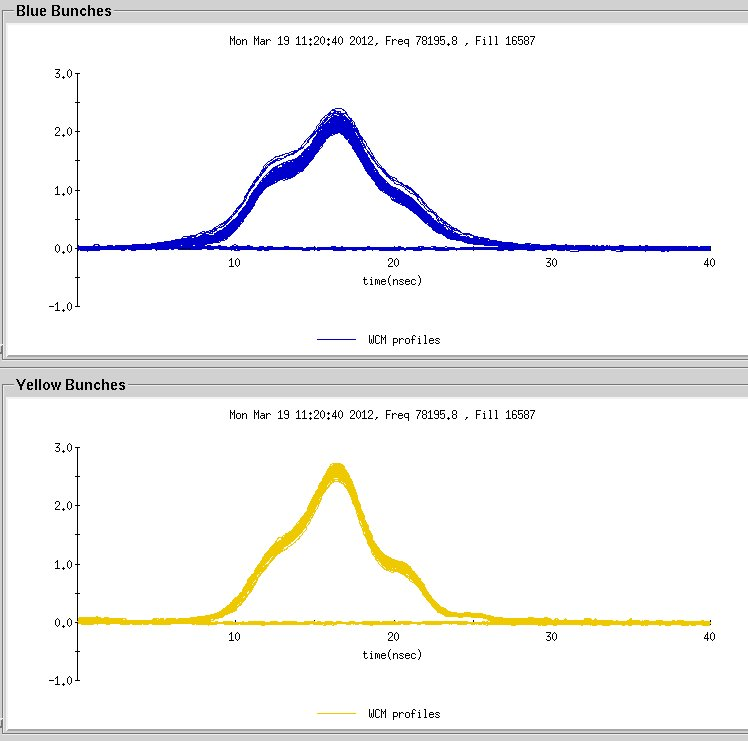
\includegraphics[width=0.7\linewidth]{./figures/wcm_16587.jpeg}
  \caption{
		The longitudinal distribution of all bunches in a typical fill are overlaid.
		The bunches from the blue beam (top) and yellow beam (bottom) are shown for
		over a 40 nanosecond time period. 
  }
  \label{fig:bunch_profile_overlay}
\end{figure}

\clearpage
\section{Production of Polarized Proton Beams}

\textbf{\textcolor{red}{Resume Here!}}

The production of polarized beams is crucial to the physics of this measurement
- without polarized beams, no spin structure analysis can be done at RHIC. This
is due to the fact that the helicity state of the protons in the initial state
of any proton proton collision can be connected to the final observed states in
a way which provides information about the spin structure function, as was
discussed in section \ref{ch:modeling_proton_spin}. 

The production of polarized beams is a multistage process, and involves several
experimental components. The importance of polarizing the beams is fully
realized once polarized beams are collided at relatively high center of mass
energies--where the beams behave less like polarized proton beams, but more
like polarized beams of quarks and gluons \cite{Alekseev2003}.  Beam
polarization is achieved incrementally--with polarization starting as soon as
the booster and AGS stage of the acceleration process \ref{fig:rhic_complex}.

The RHIC Configuration Manual \cite{RHIC2006} provides a wealth of information,
accelerator physics, diagrams, equations, and descriptions of the extremely
precise and comprehensive approach to creating polarized proton beams and
injecting them into RHIC. This work was crucial to this section of my thesis,
and is recommended reading for anyone who wishes to know `all the details' of
how RHIC handles polarized beams.

\subsection{Polarized Injection}

RHIC uses an optically pumped polarized ion source (OPPIS),
Figure~\ref{fig:rhic_oppis} to produce a polarized ion source greatly in excess
of RHIC's design intensity. This is used to our advantage, as the emittance of
the beam can be lowered to create a highly collimated beam for physics use.

\begin{figure}[ht]
	\centering
	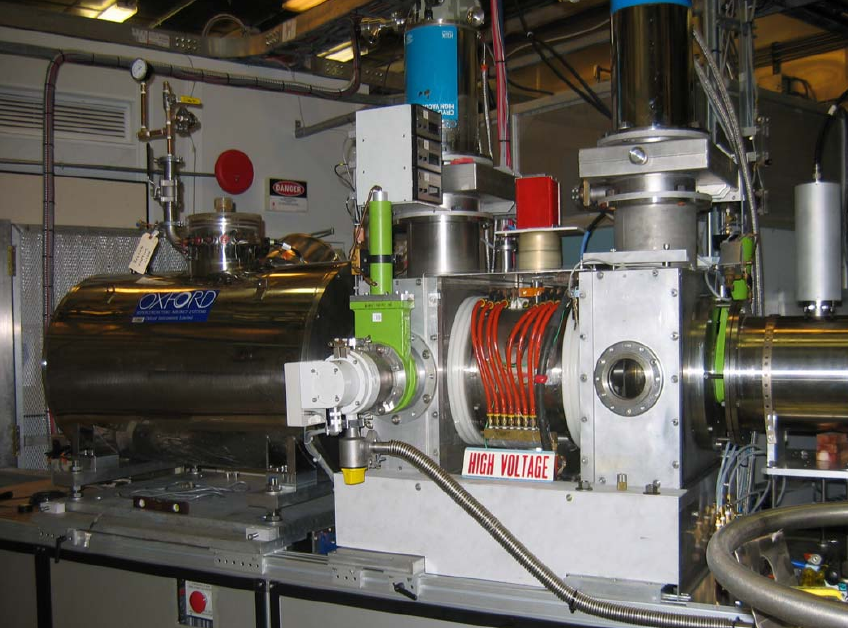
\includegraphics[width=0.8\linewidth]{./figures/rhic_oppis.png}
	\caption{
		RHIC's optically pumped polarized ion source. Produces 0.5-1.0 mA current of
		polarized $H^-$ ions. The optical pumping is pulsed at 400
		$\mu$s, \cite{Zelenski2007}
	}
	\label{fig:rhic_oppis}
\end{figure}

\clearpage
\subsection{AGS to RHIC Transfer Line}

\begin{figure}
  \centering
  \begin{subfigure}[b]{\textwidth}
    \centering
    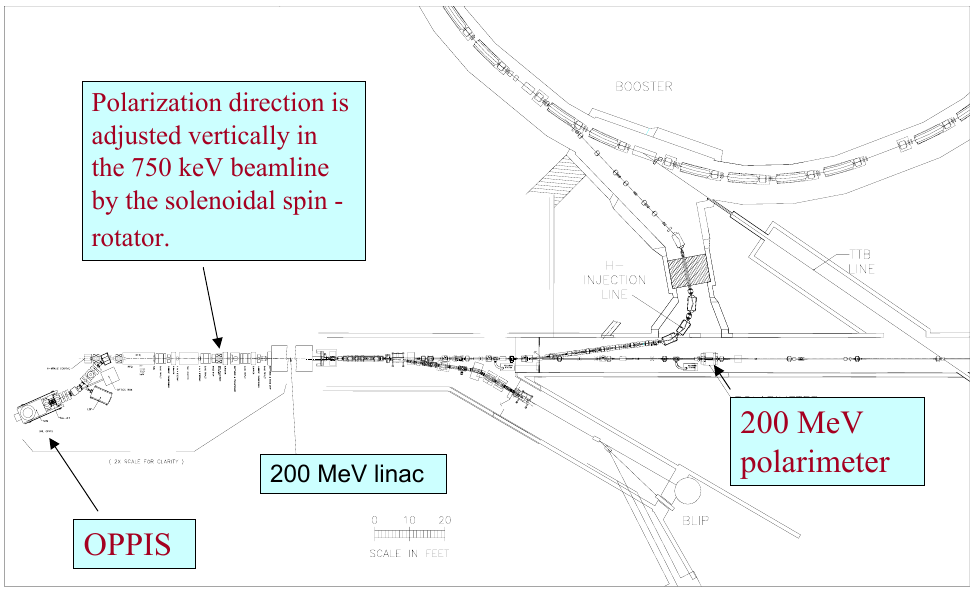
\includegraphics[width=0.7\linewidth]{./figures/rhic_polarized_injector.png}
		\caption{
			Technical schematic of Polarized Injection Line \cite{Zelenski2007}
		}
    \label{fig:polarized_top_view_1} 
  \end{subfigure}
  \begin{subfigure}[b]{\textwidth}
    \centering
    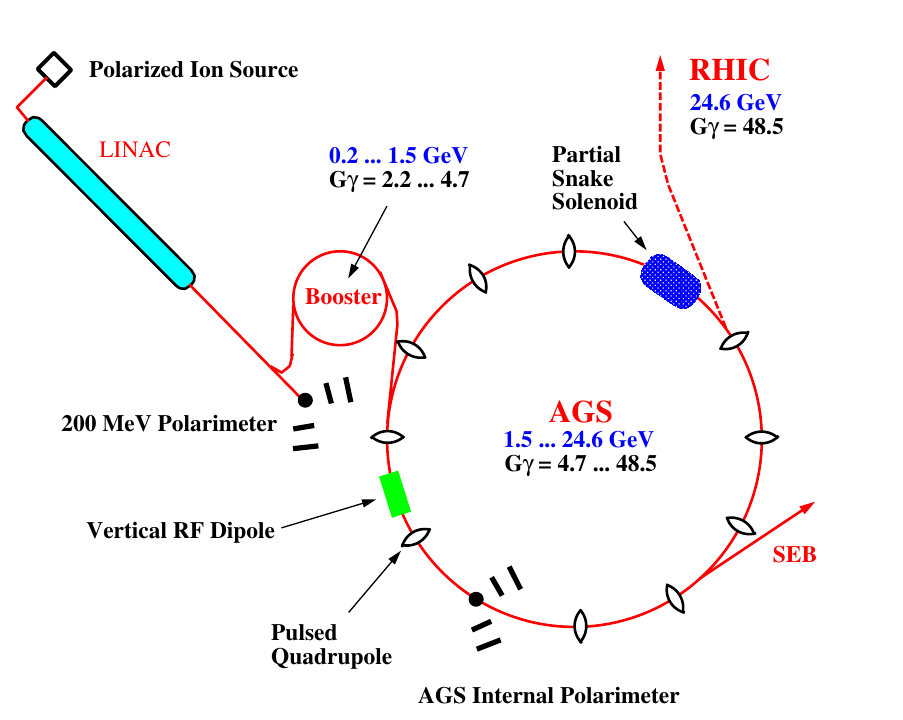
\includegraphics[width=0.7\linewidth]{./figures/polarized_beam_rhic_complex.png}
		\caption{
			Overhead view of Polarized Injection Line \cite{RHIC2006}
		}
    \label{fig:polarized_top_view_2}
  \end{subfigure}
  \caption{
		A view of the RHIC polarized injection system. We see a zoomed in technical
		view of the OPPIS to the booster (a), below, we see a zoomed out cartoon of
		the next step in the polarization injection system, including the AGS, and
		the feeder line to RHIC.
  }
  \label{fig:rhic_polarized_beam_line}
\end{figure}

Once ions have been optically pumped, we have a direct-current beam at
approximately 80\% polarization. The pumping is accomplished using Rubidium
vapor. The polarized ions are then moved into the booster from the Linac, where
some polarization is lost to spin precession, intrinsic to accelerating charged
ions in a circular path. However, polarization is maintained, for the most part,
by matching the precession resonance to the orbiting frequency of the booster
ring. The Siberian snakes and spin rotators at this stage serve to incrementally
flip the ion spin such that the natural depolarization works to re-polarize the
orbiting ions, every full-turn. The full details of this procedure are well
described in \cite{RHIC2006}.

After the ions are sufficiently polarized and filled in the AGS, they are moved
into the AGS to RHIC Transfer line, Figure~\ref{fig:ags_to_rhic}. The beam is
focused and fed through a switching magnet--which must be timed with great
precision in order to fill the blue and yellow beams with the appropriate
polarization patters. In fact, the precision is so great, that the earth's
curvature must be taken into account over this relatively short injection line -
the entry point and exit point are bent ever slow slightly different--the entry
being 12.51 mrad, vs the egress being 12.46 mrad \cite{RHIC2006}. At the point
of injection in the transfer line, the beam size and emittance are measured, as
well as the beam polarization. 

\begin{figure}
  \centering
  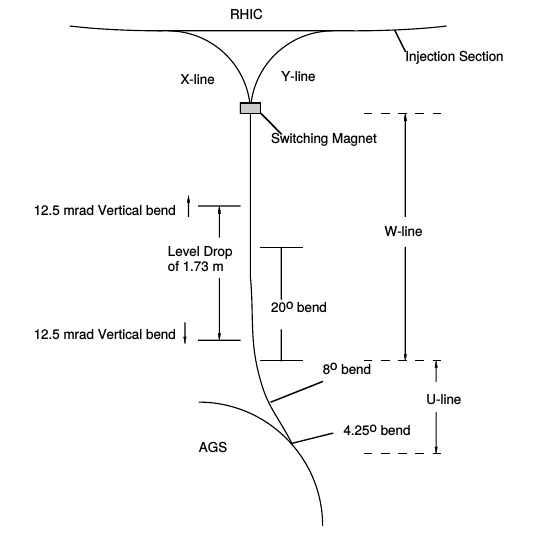
\includegraphics[width=0.6\linewidth]{./figures/ags_to_rhic_transfer}
  \caption{
    A schematic of the geometry of the AGS-to-RHIC transfer line~\cite{RHIC2006}.
  }
  \label{fig:ags_to_rhic}
\end{figure}

\clearpage
\section{Maintaining Beam Polarization}
\label{sec:beam_polarization}

The creation of polarized beams is only half the battle. Depolarizing resonances
in any particle beam are intrinsic in the design of any circulating beam
particle accelerator--without intervention, after a few rotations, RHIC's
polarized beams would be unpolarized. RHIC uses several strategies in concert to
correct for the largest of these depolarizing resonances--including beam orbit
corrections, the Siberian Snakes, Betatron Tune Spreading, and sextupole
magnetic depolarizing resonances. 

\subsection{Siberian Snakes and Spin Rotators}

The Siberian Snakes are positioned at two locations on the RHIC ring (as well as
others along the injection sequence). The most stable configuration of spin
injected in RHIC is such that the spin axis is perpendicular to the plane of the
accelerator ring. The Siberian snake is a helical magnet which forces the spin
to rotate 180 degrees every half rotation. This special configuration of snakes
(see Figure~\ref{fig:rhic_complex}) ingeniously takes advantage of the
rotational precision of the spin (a depolarizing resonance) to re-polarize the
beam, every half-orbit.

The spin rotators are located outside of experimental interaction regions around
PHENIX and STAR. These special dipole magnets rotate the spin of the beams onto
a longitudinal (parallel with beam) axis--these magnets are important for any
measurement (such as this one) requiring longitudinal spin polarization.
Otherwise, transverse spin effects can by studied.

\subsection{Measuring Beam Polarization}

The RHIC Collider-Accelerator Department provides several means of measuring the
beam polarization over the course of the data taking period. PHENIX takes
special data and studies it, to determine the real beam polarization delivered
to the detector, in a yearly analysis (for years where polarized data is taken).
This analysis is often called ``Local Polarimetry'', but is often abbreviated as
LPol in PHENIX logs.

CAD will additionally measure polarization in via inelastic proton-carbon
scattering in the Coulomb-Nuclear Interference (CNI) region. Relative
polarization can be determined with to within 10\% in only a few seconds of
measurement. 

Vertical polarization is determined through the calculation of the left and
right particle production, with a known analyzing power (\cite{RHIC2006}, Ch 8):

\begin{equation}
  P_B = {{1}\over{A_p}}{{N_L-N_R}\over{N_L+N_R}}
  \label{eq:rhic_polarization}
\end{equation}

Where $P_B$ is the beam polarization, $N_L$ and $N_R$ are the left-scattering
produced particles, and right-scattering produced particles and $A_p$ is the
analyzing power, which can be calculated from first principals, and
experimentally verified. Scattering takes place as a carbon filament is swept
across the beam.

As many decisions are financially constrained, this one was too. Using a
p-Carbon CNI polarimeter provides an economically viable way to measure beam
polarization within the precision needed for the spin experiments.

\subsubsection{The Spin Monitor}
\label{sec:the_spin_monitor}

One of my major contributions to the PHENIX experiment was in the upkeep and
development of the spin monitoring systems for the online data taking portions
of the experiment.

During a RHIC run, it is crucial to keep track of the polarization patterns
being collided at the PHENIX IR~\ref{fig:phenix_spin_collision}

\begin{figure}
  \centering
  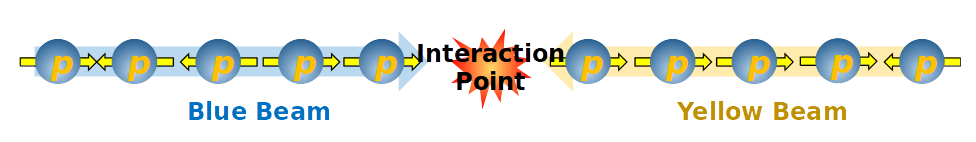
\includegraphics[width=\linewidth]{./figures/phenix_spin_collision}
  \caption{
    As beams are longitudinally rotated into position for collision, it is
    crucial to keep careful track of the magnet currents rotating the beams, as
    well as the overall polarization pattern. Shown is a carton of one potential
    polarization pattern.
  }
  \label{fig:phenix_spin_collision}
\end{figure}

The spin monitor was composed of tens of thousands of lines of code, and was
quite a monstrosity to keep running, however, I managed it. I contributed better
error logging, and helped to facilitate a total rewrite of the software, to
create more understandable and reliable output. However, in the interim, I
reprogrammed the monitor to handle spin patterns, and provide the shift crew at
PHENIX with immediate feedback regarding the spin-quality of the live data,
Figure~\ref{fig:spin_monitor}

\begin{figure}
  \centering
  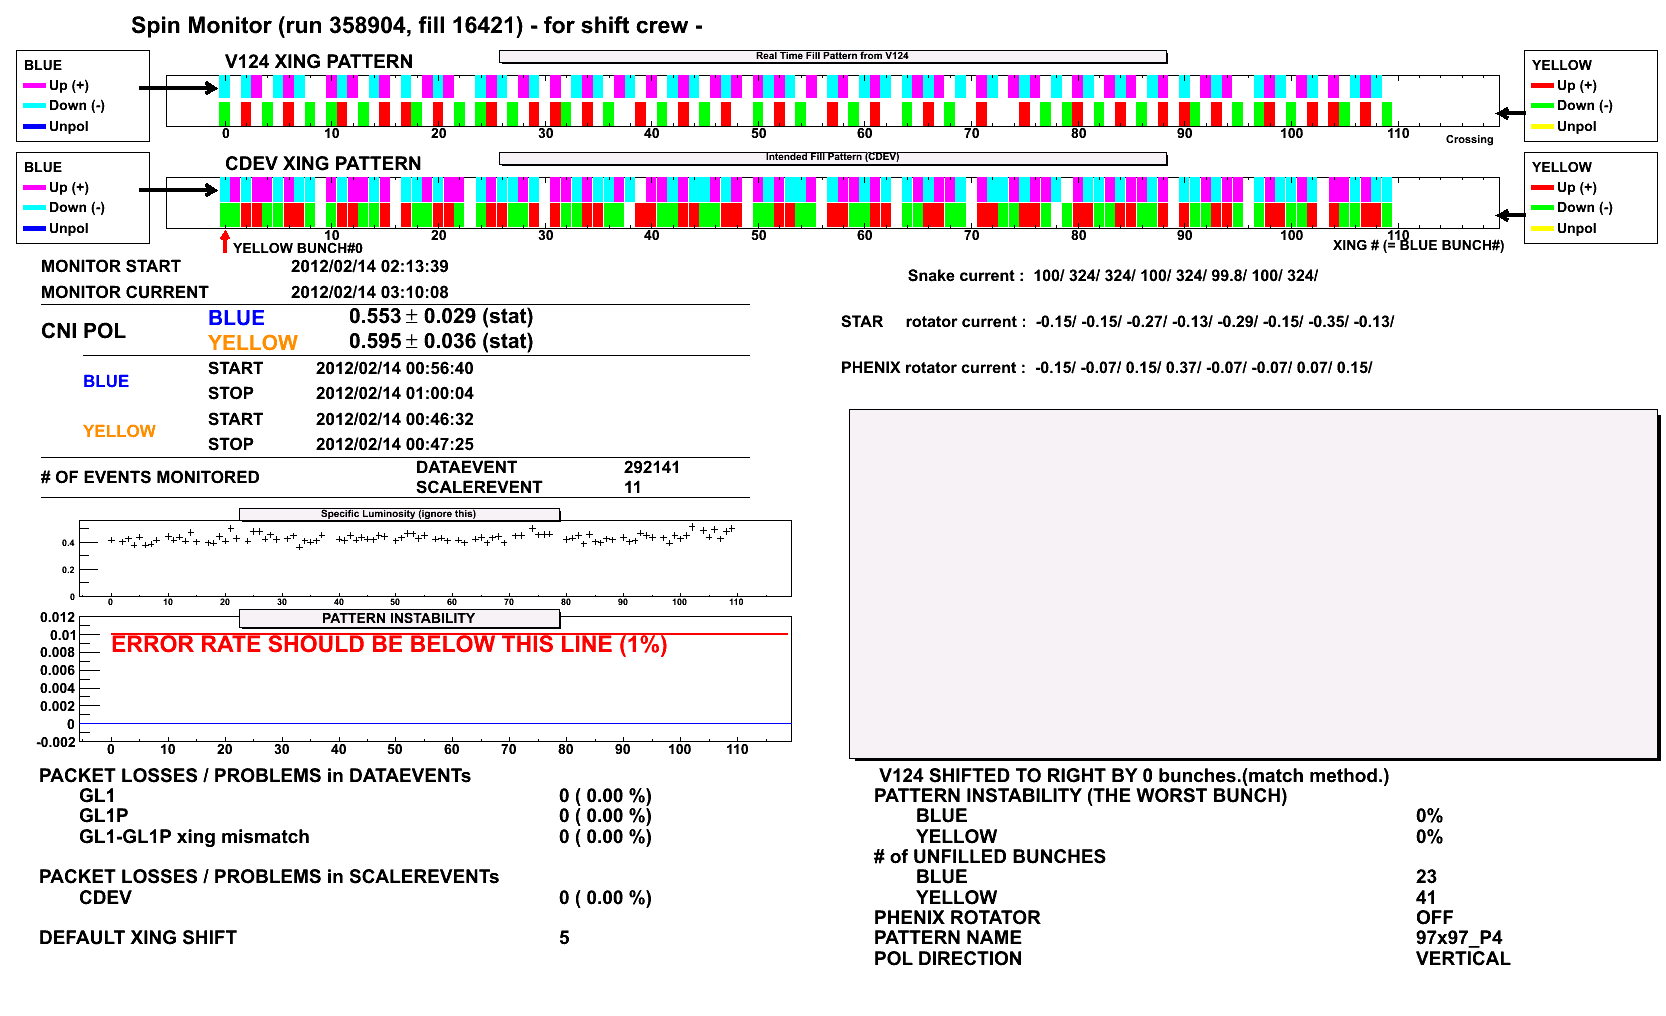
\includegraphics[width=\linewidth]{./figures/SPINMON_shift_358904.png}
  \caption{
    The shift-crew display output for the Spin Monitor. The upper panel shows
    the polarization of the blue and yellow beams, and other panels summarize
    information including magnet currents (needed to understand the spin
    orientation), issues with data packet loss, the recognized spin-pattern, as
    well as a large boxed area on the lower left where errors could be shown to
    the shift crew along with the proper response.
  }
  \label{fig:spin_monitor}

\end{figure}


\clearpage
\section{The Pioneering High Energy Nuclear Interaction Experiment}
\label{sec:PHENIX}
The Pioneering High Energy Nuclear Interaction Experiment is a synthesis of many
smaller detectors all of whom were commissioned for various physics goals, some
of which have been repurposeed from their original application once the primary
physics mission of the detectors were completed.

The configuration of the PHENIX spectrometer can be changed from year to year,
depending on the analysis needs of the physics working groups. The configuration
of the detector for the 2013 physics run is shown in
Figure~\ref{fig:phenix_2013_config}.

\begin{figure}
  \centering
  \begin{subfigure}[t]{\textwidth}
    \centering
    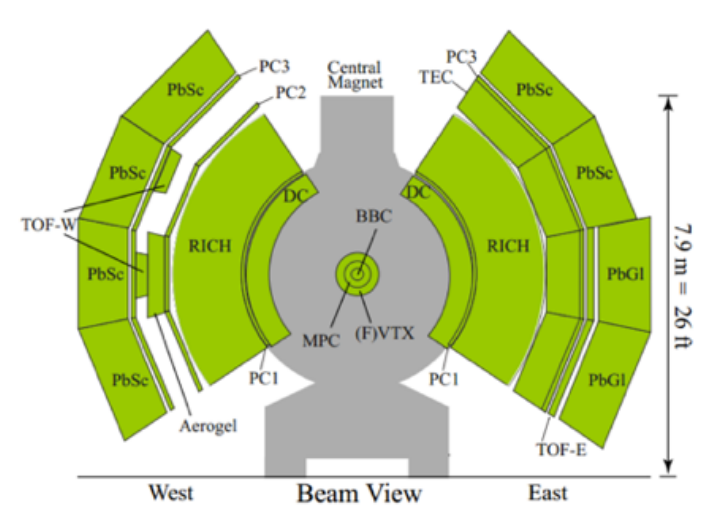
\includegraphics[width=0.8\linewidth]{./figures/phenix_2013_config_central_arms}
    \caption{Central Arms}
    \label{fig:phenix_central} 
  \end{subfigure} 
  \begin{subfigure}[t]{\textwidth}
    \centering
    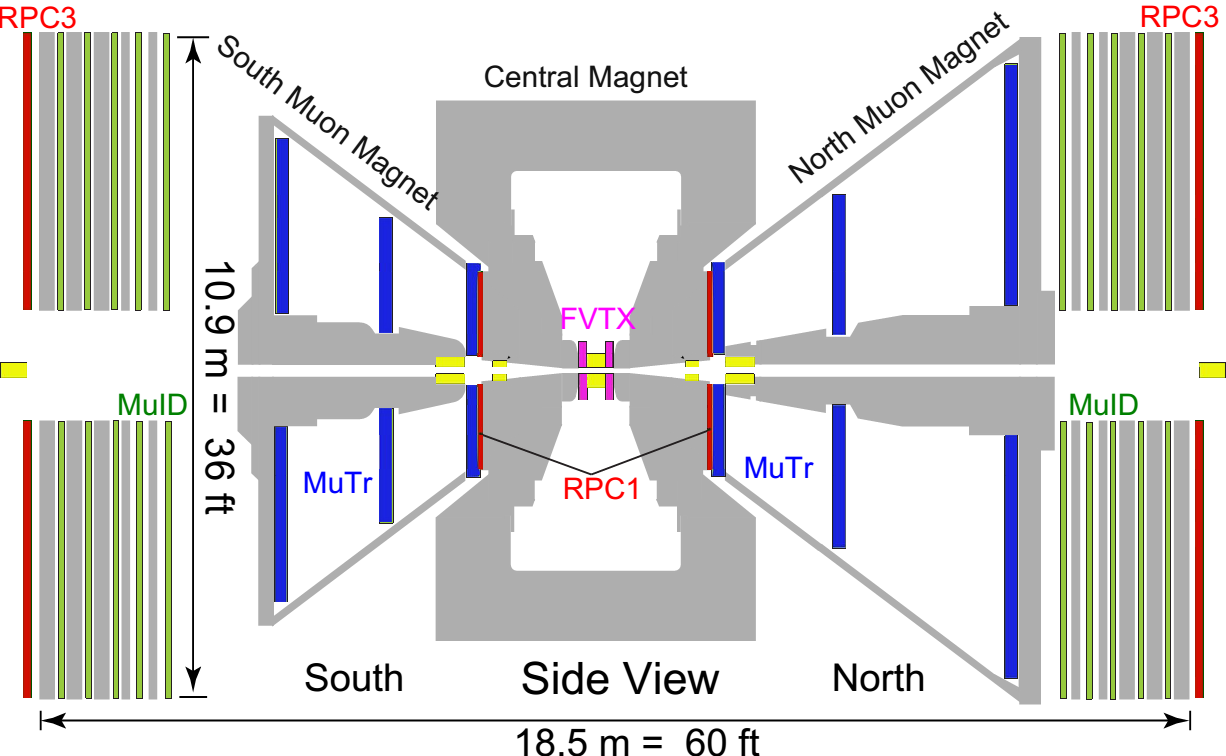
\includegraphics[width=0.8\linewidth]{./figures/phenix_2013_config_muon_arms}
    \caption{Forward Muon Arms}
    \label{fig:phenix_forward}
  \end{subfigure}
  \caption{
    Shown: The two main halves of the PHENIX Spectrometer. The central arms are
    shown via the beam-on view of PHENIX (left) and Forward Muon Arms are shown
    via the 90-degree rotated view. In both cases, the 2013 configuration is
    shown. The beams are brought into intersection at the geometric center of
    each figure (immediately between the BBCs)
  }
  \label{fig:phenix_2013_config}
\end{figure}

PHENIX makes use of many classic detector technologies, it contains \v{C}erenkov
light detectors, resistive plate chambers, electromagnetic calorimeters, silicon
chip detectors, time of flight detectors, scintillation light detectors, cathode
strip chambers, and proportional tube counters.

While all of these subsystems are interesting, and have produced excellent
physics results, I will focus only on those pertinent to this analysis.

PHENIX is generally thought of as two `halves', which often are used in separate
analyses--the forward muon arms, and the central arms. While both halves are
used for both heavy ion, and spin physics analyses, this analysis exclusively
uses the forward muon arms, so the central arms will not be discussed (though, a
closely related analysis, dealing with $A_L$ for $W\rightarrow e$ exclusively
uses the central arms). The different subsystems cover different rapidity
ranges, so many times, complimentary results are obtained from central and
forward analysis. Results from such a complementary central analysis will be
presented alongside my results in later chapters.

PHENIX also utilizes a complex data acquisition system (DAQ) which streams data
from each detector, assembles this data into a labeled event, compresses and
stores into a proprietary storage format, the work-flow of this is summarized in
Figure~\ref{fig:phenix_daq_overview}. A complete summary of PHENIX detector
subsystems (excluding the Forward Vertex Detector, Silicon Vertex Detector, and
Resistive Plate Chambers, which are new, and discussed separately) can by found
in Table~\ref{tab:phenix_detector_summary}.

\begin{figure}
  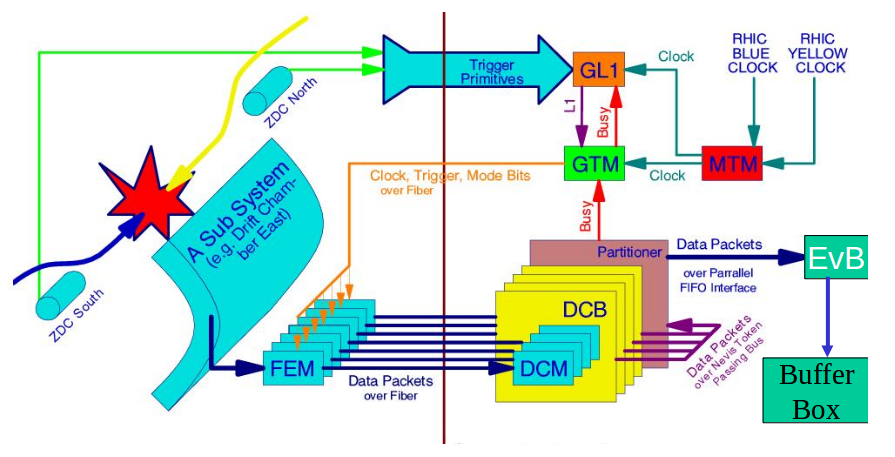
\includegraphics[width=\linewidth]{./figures/daq_overview}
  \caption{ 
    A flow chart summarizing the PHENIX DAQ \cite{Desmond2016}. From left to
    right, we can get a feel for the data flow at PHENIX. Shown is an event, the
    red splat on the far left. Particles from this event are transduced by a
    detector (`A Sub System'). The transduced signals are serialized into a
    detector specific data stream, such that the state of the detector's
    excitation can be recorded and reproduced later. This information is stored
    on the front-end-electronics modules (FEMs), and synchronized with timing
    information from the clock (ticks once every time there is a bunch crossing)
    and a Global Trigger decision, i.e. whether or not the right parts of the
    detector lit up to make this particular event worth keeping. After this, if
    the event is deigned by the heuristics to be worthy of keeping, the
    uncompressed serialized information is sent to the DCMs, where it is
    assembled into a packet, and then sent to the event builder (EvB), where all
    packets sharing a common collision are assembled into an event. The event is
    compressed into a proprietary PRDF format, and sent to the Buffer Boxes,
    which are a cache of high density local storage, which is later sent off to
    cold storage on magnetic tape drives.
  }
  \label{fig:phenix_daq_overview}
\end{figure}

\begin{table}
  \centering
  \begin{tabular}{l c c l}
    \toprule
    \textbf{Element}	& \textbf{$\Delta\eta$}	& \textbf{$\Delta\phi$} & \textbf{Features} \\
    \midrule
    \textbf{Magnets} & & & \\
    Central Magnet & $\pm 0.35$ & $360^{\circ}$ & 1.15 $T$ \\ 
    Muon Magnet North & $-1.1$ - $-2.2$ & $360^{\circ}$ & 0.72 $T$ \\
    Muon Magnet South & $1.1$ - $2.4$ & $360^{\circ}$ & 0.72 $T$ \\
                      & & & \\
    \textbf{Minimum Bias} & & & \\
    Beam Beam Counter & $\pm(3.1-3.9)$ & $360^{\circ}$ & Vertex Reconstruction \\
    Zero Degree Calorimeter & $\pm 2 mrad$ & $360^{\circ}$ & Minimum Bias Trigger \\
                            & & & \\
    \textbf{Central Detectors} & & & \\
    Drift Chambers & $\pm0.35$ & $90^{\circ}\times2$ & Central $p$ and $m$ resolution \\
    Pad Chambers & $\pm0.35$ & $90^{\circ}\times2$ & Pattern Recognition, Tracking \\
    Ring Imaging \v{C}erenkov & $\pm0.35$ & $90^{\circ}\times2$ & Electron ID \\
    Time of Flight & $\pm0.35$ & $45^{\circ}$ & Hadron ID, $\sigma<100pm$ \\
    PbSc EMCal & $\pm0.35$ & $90^{\circ}$, $45^{\circ}$ & Calorimetry, photon, \\
               & & & and electron energy \\
    PbGl EMCal & $\pm0.35$ & $45^{\circ}$ & $e^{\pm}$, $\mu^{\pm}$ separation at $p> 1 GeV/c$ \\
               & & & EM Shower and $p < 0.35 GeV$, $K^{\pm}$ \\
               & & & $\pi^{\pm}$ separation up to $1 GeV/c$  \\
               & & & \\
    \textbf{Muon Arms} & & & \\
    Muon Tracker South & -1.15 to -2.25 & $360^{\circ}$ & North installed 2003 \\
    Muon Tracker North & 1.15 to 2.44   & $360^{\circ}$ &  \\
    Muon ID South & -1.15 to -2.25 & $360^{\circ}$ & Steel absorbers, larocci tubes \\
    Muon ID North & 1.15 to 2.44   & $360^{\circ}$ & "" \\
    \bottomrule 
  \end{tabular}
  \caption{
    A summary of PHENIX hardware~\cite{Adcox2003}. Electron/pion separation and
    Pion/Kaon separation requires the Time of Flight (ToF) working with PbGl and
    PbSc data. PbGl refers to ``Lead Glass Scintillator'' and PbSc refers to ``Lead
    Scintillator''. The Muon Identifier (Muon ID, MuID) can help separate muons
    from hadrons. 
  }
  \label{tab:phenix_detector_summary}
\end{table}

\subsection{The Spin Program}
The PHENIX spin program was planned as part of the RHIC upgrade to produce
polarized proton beams. The major analysis thrust of the PHENIX spin program has
been to understand the spin structure of the proton, and has historically used
various flavors of particle production asymmetries (left-right and
forward-backward) as an experimental probe for polarized parton distribution
functions (as we saw in Chapter~\ref{ch:modeling_proton_spin}).

Much of PHENIX collaboration's early published work focused on creating and
studying quark gluon plasma in heavy ion collisions, but in following years spin
papers came too. Major question in physics that PHENIX set out to answer with
its heavy-ion program include studying confinement--i.e.  why are quark color
charges confined to exist in the nucleus, baryons and mesons? PHENIX sought to
study this via examination of the J/$Psi$ and measuring screening length in
heavy ion collisions. Additional research topics included the study of chiral
symmetry restoration, thermal radiation of hot gasses, QCD Phase transition,
Strangeness and Charm Production, Jet Quenching, and Space-time
evolution~\cite{Nagamiya1994} .

The spin program came shortly after the 2001 commissioning run. The first
polarized proton run was produced by RHIC for PHENIX in 2002, with 8.3 total
weeks of data, run discontinuously. The primary goals of the PHENIX spin
program are to study the polarization of the proton, specifically in the context
of the Ellis-Jaffe sum rule, which decomposes the proton spin into various
contributions from its substructure. The main structures studied by PHENIX are
the gluon polarization, $\Delta g$ and the anti-quark polarization, $\Delta
\bar{q}$. Additionally, the 'nature of parity non-conservation itself can be
directly studied' using polarized beams, and spin asymmetries in collisions.
Though this measurement generally requires a means of reconstructing jets
(PHENIX doesn't have this), inclusive or leading particle production can be used
as a substitute with some small asymmetry
remaining~\cite{PHENIXCollaboration1998}.

\subsection{Subsystems}

The major subsystems contributing to this work include the Muon Arms, the Beam
Beam Counters (BBCs), and the Forward Vertex Detector, since the analysis is
totally characterized with calculating the $A_L$ for $W\rightarrow\mu$
interactions, only muon reconstruction and identification is required. The
Central arms are used in the $W\rightarrow e$ analysis. 

\subsubsection{Beam Beam Counters}

The Beam-Beam counters (BBCs, Figure~\ref{fig:bbc_overview}) are photomultiplier
tubes with scintillating lead-glass crystals. These detectors are situated about
144 cm on either side of the nominal center of the PHENIX interaction region,
and typically are used to trigger on events with minimal bias towards any
particular physics goal. This is important as a means for reconstructing the
relative abundance of particle production, which is as you might expect, crucial
for determination of any inelastic scattering cross section. The Beam-Beam
counters provide us with vertex reconstruction by way of analyzing the time
delay between triggering of the North BBC and the South BBC. The delay window is
then used to reconstruct the event vertex by assuming particles are traveling
at near light speed, Figure~\ref{fig:bbc_vertex_reconstruction}. 

\begin{figure}[ht]
  \centering
  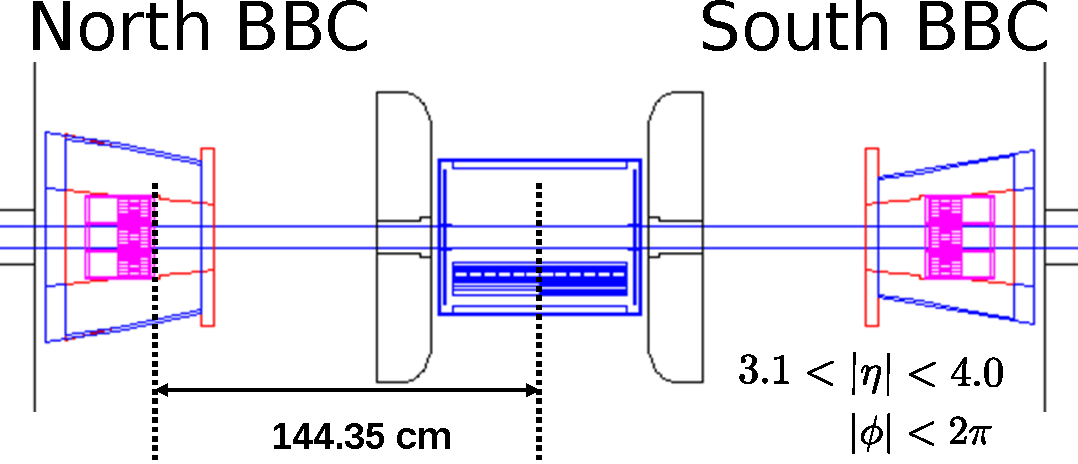
\includegraphics[width=\linewidth]{./figures/bbc_overview}
  \caption{
    Shown: a photograph of the BBC hugging the beryllium beam pipe near the
    center of PHENIX (top left), a schematic showing the relative size and
    location of the BBCs as compared to the rest of PHENIX (top right), and a
    schematic of the exact proportions of the detector as viewed alongside the
    beam pipe (bottom), along with the rapidity and azimuthal
    coverage~\cite{Nakamura2002}
  }
  \label{fig:bbc_overview}
\end{figure}

\begin{figure}[ht]
  \centering
  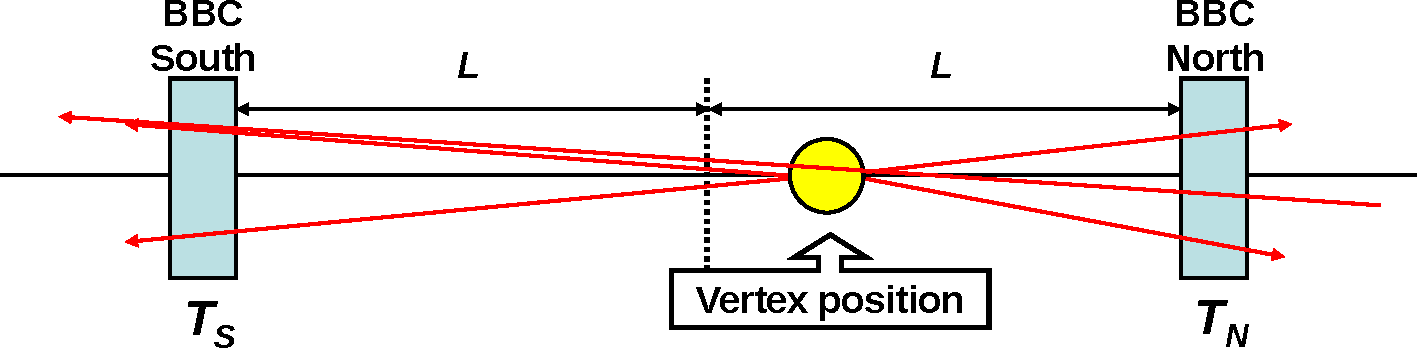
\includegraphics[width=\linewidth]{./figures/bbc_vertex_reconstruction}
  \caption{
    A diagram outlining the strategy for reconstructing the event z-vertex of a
    collision. Top: a cartoon of the North and South BBCs getting some particle
    penetration after an event. Bottom Right: a characteristic distribution of
    measured z-vertices for a short run taken in 2002~\cite{Nakamura2002}.
  }
  \label{fig:bbc_vertex_reconstruction}
\end{figure}


\clearpage
\subsubsection{Forward Vertex Detector}

The Forward Vertex Detector, Figure~\ref{fig:forward_vertex_detector} is a
silicon detector, which provides additional tracking to detect secondary event
vertices and additional precision to the Muon Tracking system. This detector can
provide an important additional layer of precision, because it can help to
identify events which do not originate from the primary event vertex of a
collision, so they can be rejected from a pool of candidate $W\rightarrow\mu$
events~\cite{Aidala2014}. The properties of this detector are summarized in
Table~\ref{tab:fvtx_properties}

\begin{table}[ht]
  \centering
  \begin{tabular}{lc}
    \toprule
    \textbf{Property} & \textbf{Value}\\
    \midrule
    Silicon sensor thickness ($\mu$m) &	320\\
    Strip pitch ($\mu$m) &	75\\
    Nominal operating sensor bias (V)	& +70\\
    Strips per column for small, large wedges	& 640, 1664\\
    Inner radius of silicon (mm) &	44.0\\
    Strip columns per half-disk (2 per wedge) &	48\\
    Mean z-position of four stations (mm)	& ±201.1, ±261.4, ±321.7, ±382.0\\
    Silicon mean z offsets from station center (mm) & 	±5.845, ±9.845\\
    \bottomrule
  \end{tabular}
  \caption{
    A brief summary of the FVTX design parameters~\cite{Aidala2014}
  }
  \label{tab:fvtx_properties}
\end{table}

\begin{figure}[ht]
  \centering
  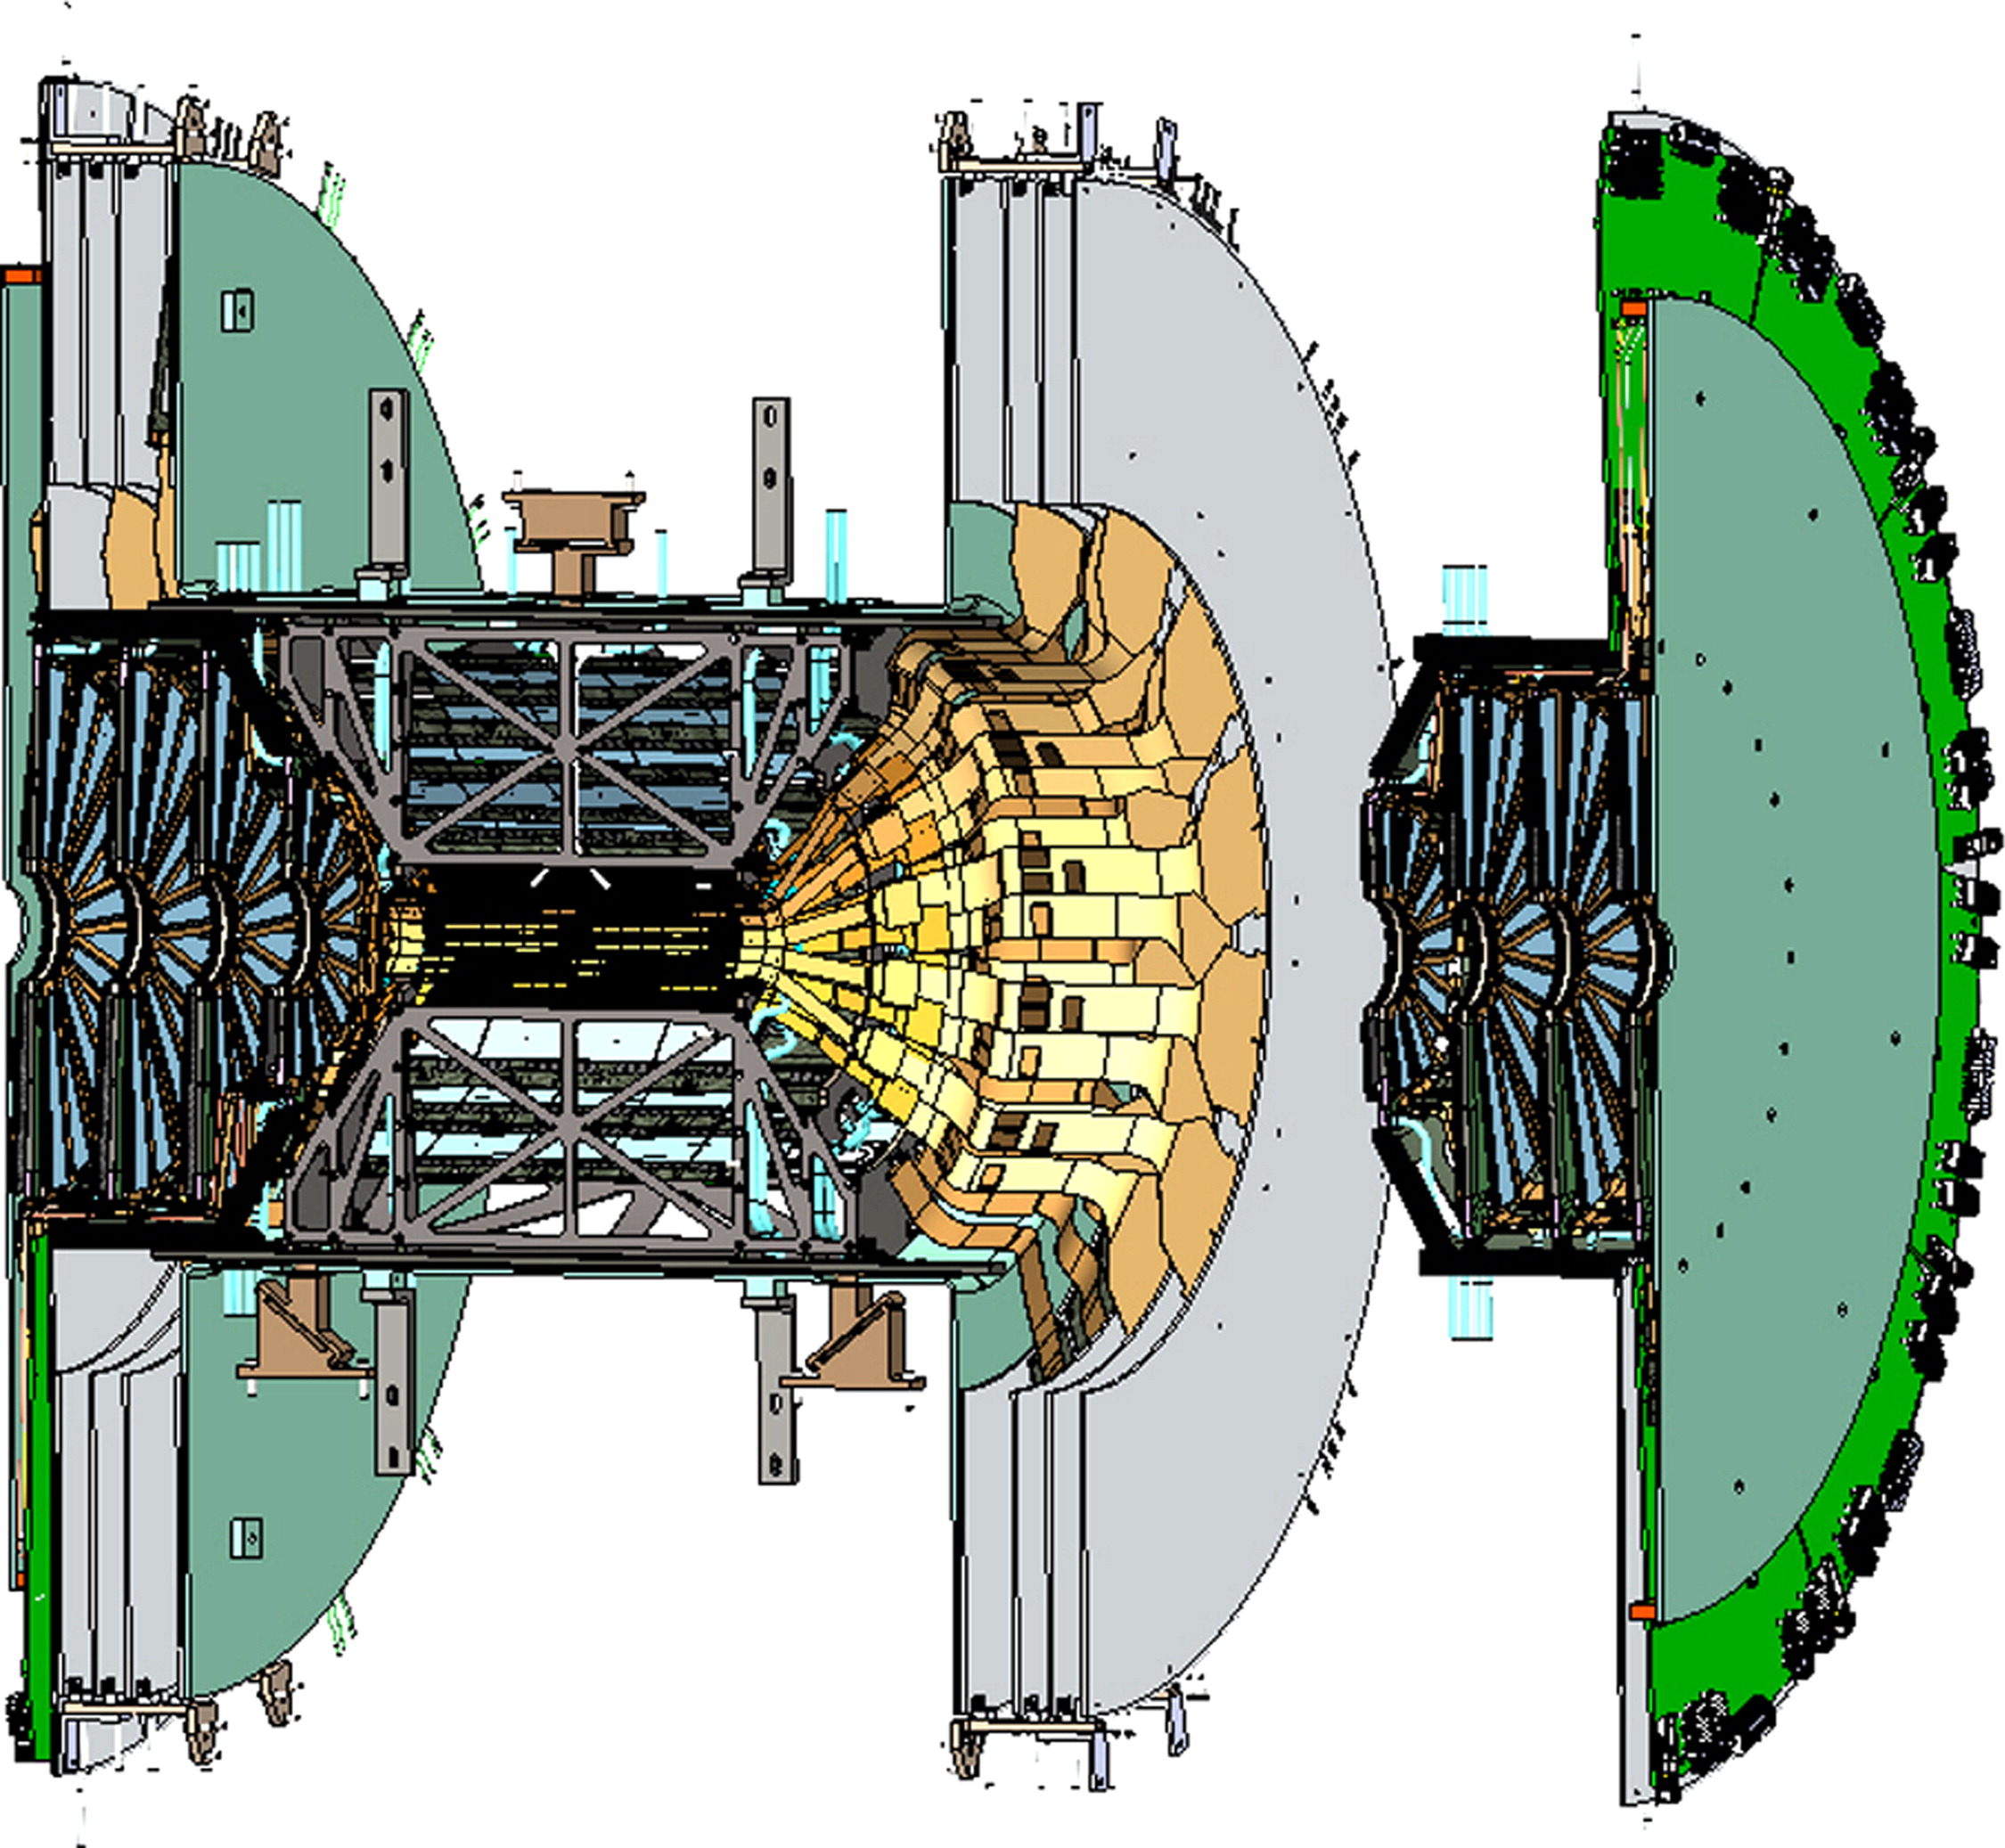
\includegraphics[width=0.6\linewidth]{./figures/forward_vertex_detector}
  \caption{
    A schematic of the Forward Vertex Detector, showing the silicon chip layers
    (light blue wedges), and readout electronics (green). They are mounted
    directly onto the Silicon Vertex Detector, which was not used in this
    analysis. The FVTX and SVD together are used in heavy ion
    analyses~\cite{Aidala2014}.
  }
  \label{fig:forward_vertex_detector}
\end{figure}


\clearpage
\subsubsection{The Muon Arms}

The Muon Arms are composed of several subsystems, including the Muon Tracker
(MuTR, cathode strip chambers), the Muon Identifier (MuID, shielding and
scintillation layers), and the Resistive Plate Chambers (RPC(s), bakelite gas
gaps and azimuthal oriented capacitively coupled copper readout strips). The job
of the muon tracker is to identify muons with the penetration through the many
layers of the MuID, and provide momentum and charge reconstruction for muon
tracks. Tracks are matched to the event vertex with Kalman filter during
reconstruction, and can even be matched with FVTX secondary vertices as a means
of rejecting non W-Boson decays. Prior to the Forward Upgrade
(Section~\ref{sec:forward_upgrade}), the muon arms consisted solely of the Muon
Tracker and the MuID. 

The Muon Tracker has a radial magnetic field, leading to charged particles
traversing the tracker to have a helical bend. This was suitable for lower
energy muon tracks, such as muons coming from the J$\Psi$ decay, which was one
of the primary decays targeted in the original design of the muon tracker.

However, these J/$\Psi$ muons have much lower energy then muons which decay from
areal W-Boson production. To extend the muon tracker's usefulness into tracking
these high energy muons, an upgrade to the triggering system was required to
obtain adequate back-ground rejection for the Forward W analysis. The details of
the muon arms will be discussed in the next section.

\clearpage
\section{The Forward Upgrade} 
\label{sec:forward_upgrade}

The muon arms were the subject of significant upgrades from 2011-2013.
New front end electronics were added to improve triggering, and entire new
detector subsystems (The RPCs) were added. The full details of these subsystems
will be discussed in the forthcoming sections (Section~\ref{sec:forward_upgrade}).

One of the main stated physics goals of PHENIX is to constrain the sea-quark
polarization of the proton spin. While this contribution is
expected to be small, it is not because it is expected to be uniformly zero.
Instead, the expectation is that the matter contribution to the quark sea is
strongly positively polarized, while the antimatter contribution is strongly
negatively polarized~\cite{Aidala2005}. Measuring this polarization via $A_L$
(Equation~\ref{eq:w_production_asymmetry}) is the means by which we will
accomplish this. Prior to the Forward Upgrade, we only had results from the
Central $W\rightarrow\mu$ analysis, but to better constrain our models, we
require lower uncertainty in the forward kinematic regime--thus, the Forward
Upgrade.

The first data for this measurement was taken in 2009, and published in 2010
under \cite{Adare2010} and \cite{Okada2010}, but only for central rapidities,
where a clear Jacobean peak could be found in the electron invariant mass
spectrum at 40$GeV$ mass-energy (half the rest mass of the W-Boson). This made
evaluating yields and calculating asymmetries relatively straight-forward. 

However, in forward kinematic regimes, it was very difficult to discriminate
real $W\rightarrow\mu$ from other sources $X\rightarrow\mu$. As one can observe
in Figure~\ref{fig:muon_production_vs_pt}, only at high $p_T$ does the W-boson
signal become dominant. The old muon trigger electronics did not allow
triggering sufficiently close to the W-Boson production threshold to allow for
enough data to be taken. This is because of how the Muon Tracker identifies the
charge and momentum of particles--which is via track bending. As tracks become
very straight (i.e. high $p_T$), the muon tracker struggles to reconstruct the
correct charge and momentum. The original Forward Upgrade called for a nose-cone
calorimeter, which would have helped greatly for particle rejection, but was
canned for budget reasons.

The Forward Upgrade to PHENIX increased the muon triggering threshold from about
2 $GeV$ to 10 $GeV$, enough to insure that all muons produced from W-Boson
decays can be recorded, with no loss of statistics. This of course is not to
say, that these events were recorded without any background processes--the
removal of the muon background was a substantial effort in this analysis,
described in Section~\ref{sec:sbr}.

\begin{figure}[ht]
  \centering
  \begin{subfigure}[b]{0.5\textwidth}
    \centering
    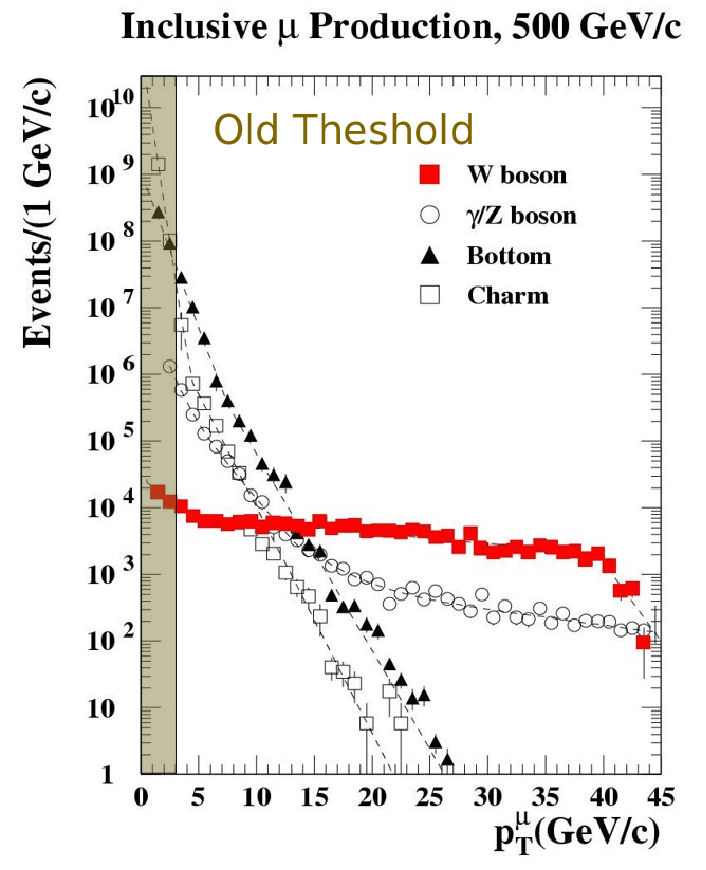
\includegraphics[width=\textwidth]{./figures/w_old_trigger.png}
    \caption{The original Muon Trigger Threshold}
    \label{fig:trig_muon_old}
  \end{subfigure}%
  ~
  \begin{subfigure}[b]{0.5\textwidth}
    \centering
    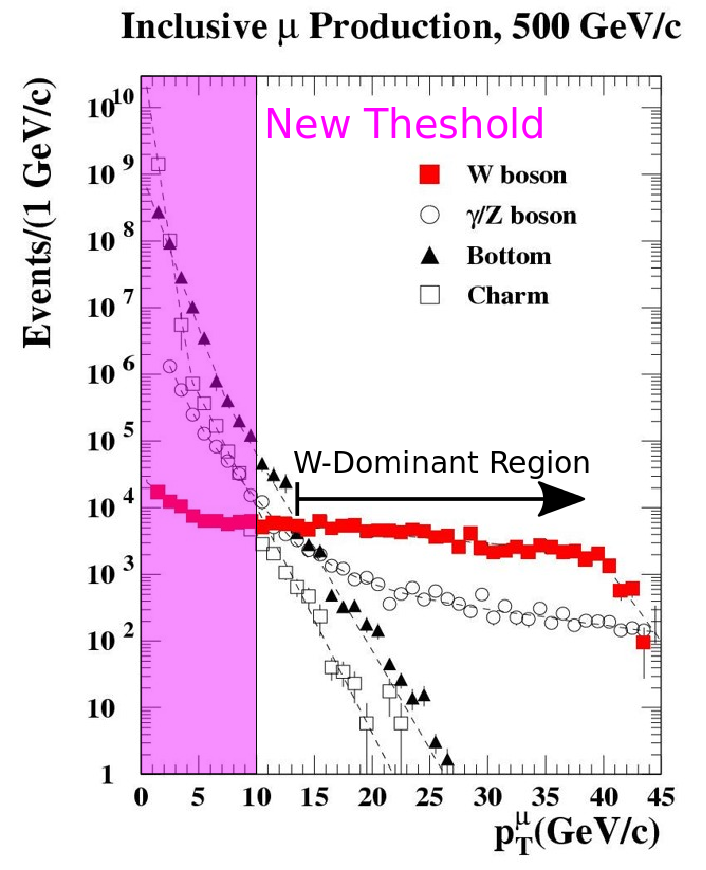
\includegraphics[width=\textwidth]{./figures/w_dominant_region_new_trigger.png}
    \caption{Muon Trigger Threshold, Forward Upgrade}
    \label{fig:trig_muon_new}
  \end{subfigure}
  \caption{ 
    Observing the simulated production of muon as a function of $p_T$, we can
    see that in the kinematic region of $W$ production that the dominant sources
    of muons come from other processes. The new PHENIX muon trigger threshold is
    sensitive at 10 $GeV/c$ and above. The threshold is still high enough that
    with other methods, we can record all events which come from the W boson,
    with triggering, whereas with the old threshold, this was impossible.
  }
  \label{fig:muon_production_vs_pt}
\end{figure}

\subsection{The Muon Tracker}

The primary purpose of the Muon Tracker is to reconstruct the energy and
momentum of muons in the forward kinematic regime. Because the MuID is composed
of larocci tubes sandwiched between solid steel sheets, only particles which
penetrate all the layers of the MuID are identified as muons. The Muon Tracker
has three cathode strip tracking planes in a volume of gas, with an applied
radial magnetic field. Each plane has two faces of tracking strips, for six
total tracking readouts total. The arrangement of cathode strips  makes the Muon
Tracker very sensitive to the azimuthal dimension, but coarsely sensitive to the
radial direction. The Muon Arms have three tracking stations for momentum and
charge identification, sandwiched between two RPCS.

Since the MuID will fire on Muons with a 2.5 $GeV$ momentum threshold, it will
trigger very rapidly at high beam energies and luminosities--too fast to record
all data--event rates were in excess of 10 MHz in 2013, with only 2 kHz of DAQ
bandwidth allocated to the W analysis. Thus, before the Forward Upgrade, the
Muon Arms were insufficient. However, additional absorber was installed at the
nose-cone of the muon tracker to block lower momentum particles. The addition of
the RPCs as well as new Front End Electronics Modules allowed for the real-time
calculation of pseudo-momentum to be fed into the trigger decision in order to
provide high rejection power on tracks. These upgrades allowed us to trigger
exclusively on relatively straight tracks, which is consistent with high
momentum particles~\cite{Fukao2011}.

\clearpage
\subsection{The Resistive Plate Chambers}

One of my major contributions to the PHENIX experiment was in the construction
and testing of the RPCs at station 1, in 2012. An exploded view of the RPC is
shown in Figure~\ref{fig:rpc_exploded}. The RPCs were a crucial part of the
W-Physics muon trigger. One primary feature the presence of RPCs add to the
PHENIX triggering system is timing resolution--2 nanoseconds
(Table~\ref{tab:rpc_design_characteristics}). This is crucial, because before
the inclusion of RPCs, the only timing available was that of the BBCs. However -
because the BBCs are minimally biased--they will fire nearly every time there
is a collision--which at high luminosity is far greater than the assigned
bandwidth to the W Physics trigger. The RPC provides local timing information,
which allows the triggering system to record events which trigger the muon arm
system, and not just the BBCs. This has the effect of significantly reducing
backgrounds--by a factor of $>$ 6000~\cite{Fukao2011},
Figure~\ref{fig:rpc_rejection_power}.

\begin{figure}
  \centering
  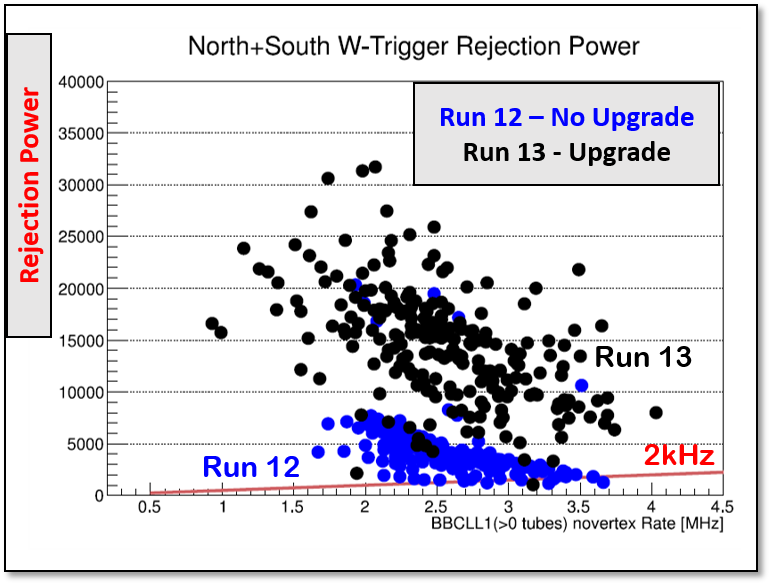
\includegraphics[width=0.8\linewidth]{./figures/rejection_power.png}
  \caption{
    In 2013 with the final commissioning of the RPCs and the Forward Upgrade
    complete, we saw a drastic increase in rejection power, as planned.
  }
  \label{fig:rpc_rejection_power}

\end{figure}


\subsubsection{Design}

\begin{figure}
  \centering
  \begin{subfigure}[b]{0.4\textwidth}
    \centering
    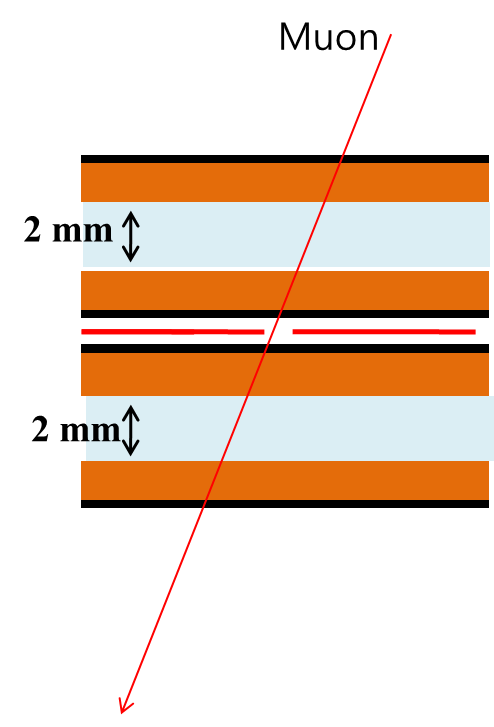
\includegraphics[width=0.8\linewidth]{./figures/rpc_1_muon_hit}
    \caption{A muon passing through the layers of the RPC}
    \label{fig:rpc_hit_side_view}
  \end{subfigure}%
  ~
  \begin{subfigure}[b]{0.4\textwidth}
    \centering
    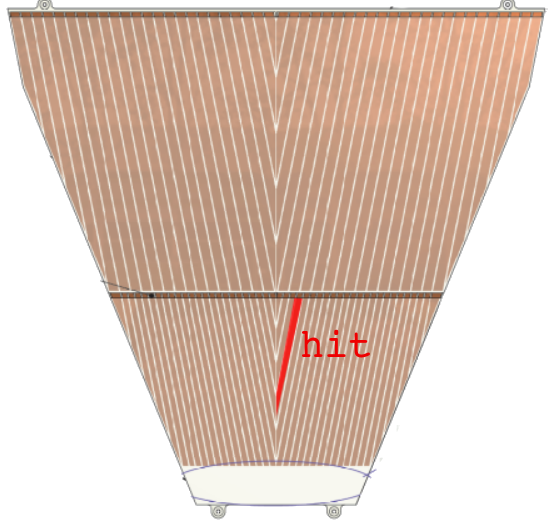
\includegraphics[width=0.8\linewidth]{./figures/rpc_1_muon_hit_side}
    \caption{Copper readout strip activated by passing muon}
    \label{fig:rpc_hit_top_view}
  \end{subfigure}
  \caption{
    As a muon passes through the layers of the RPC (left), the gas in the
    bakelite gap is ionized. This charge migrates and collects near the highly
    resistive graphite coating. An image distribution is induced on the
    overlapping readout strip (right), which is passed along its own channel to
    the front-end electronics.
  }
  \label{fig:muon_hit_rpc}
\end{figure}

As hinted at prior, the design goal of the Resistive Plate Chambers is to
provide accurate timing information at high speed in order to build a Trigger
which can record $W\rightarrow\mu$ events. RPCs were first implemented at the
Large Hadron Collider at CERN, and their design has been adopted for use at
PHENIX both because of its high speed, and low cost. In
Figure~\ref{fig:rpc_exploded} the basic design is shown--the means of signal
transduction is via ionizing of gas inside a highly resistive chamber. The
chamber is held at a large bias--at 8.5 kilovolts, such that any ionization
will collect on the interior of the resistive chamber in a fixed, and relatively
static distribution in time (relative to time scales of triggering system
timing, in millionths of a second). This charge distribution is read out by
capacitively coupled copper readout strips, into fast electronics
(Figure~\ref{fig:muon_hit_rpc}). The design requirements of PHENIX is that when
triggered, 2 or fewer clusters (strips) are activated, the efficiency of the
detector must be at least 95\%, the time resolution must be at least 2
nanoseconds, with a particle transduction rate of 500 Hz per square centimeter.
These properties are summarized in
Table~\ref{tab:rpc_design_characteristics}~\cite{Fukao2011}.

\begin{figure}[ht]
  \centering
  \includegraphics[width=0.7\linewidth]{./figures/rpc_exploded.png}
  \caption{
    We can see the various layers that go into the construction of a typical RPC
    segment installed at PHENIX. A High Voltage bias is applied to the graphite
    coating on either side of bakelite gas-filled gaps. Readout strips are
    positioned between the two bakelite gaps. Finally, the entire double-gap
    structure is surrounded by a copper grounding cage, and wrapped in
    insulating mylar~\cite{Fukao2011}.
  }
  \label{fig:rpc_exploded}
\end{figure}

\begin{table}[ht]
  \centering
  \begin{tabular}{lc}
    \toprule 
    \textbf{Cluster Size} & $<$2 strips \\
    \textbf{Efficiency} & $>$95\% for MIP \\
    \textbf{Time Resolution} & $\sim$2 nanoseconds \\
    \textbf{Rate Capability} & 0.5 kHz/$cm^2$ \\
    \bottomrule
  \end{tabular}
  \caption{
    The design characteristics of the RPCs~\cite{Fukao2011}
  }
  \label{tab:rpc_design_characteristics}
\end{table}

\subsubsection{Construction and Testing}

Construction of the Resistive Plate Chambers took place in two stages over
several years. Fabrication of the bakelite gas gaps was done overseas in Korea,
and the aluminum chassis was manufactured in China. Pieces for the RPC 3 and RPC
1 were shipped to Brookhaven National Laboratory where they were assembled and
tested, before being installed. The installation occurred over two years, with
the first stage, the RPC 3, being installed in 2011, and the second stage, the
RPC 1, being installed in 2012. After being fully commissioned, the capstone
data set for W-Physics was taken in 2013, which is discussed in detail in
Chapter~\ref{ch:data_collection}.

The RPC 3 and RPC 1 construction efforts took place in a special clean-room
built inside of the cavernous building 9-12 (Figure~\ref{fig:building_912}) at
Brookhaven National Lab. Construction was overseen by Dr. Francesca Giordano,
working as a post doctoral associate for Dr. Matthias Grosse Perdekamp for the
University of Illinois at Urbana Champagne. The electronics of the RPCs were
funded by professors Ken Barish and Rich Seto at the University of California,
Riverside, via a grant from the Department of Energy.  I am very grateful for
Francesca for her guidance and trust, as she allowed me to construct and test
many of these octants. I constructed the gaps with Arbin Timilsina, who was a
very entertaining and helpful lab-mate. Ihnjei Choi and Young Jin Kim were
instrumental in the design, construction, and QA of the RPCs as well. 

\begin{figure}
  \centering
  \includegraphics[width=0.5\linewidth]{./figures/building_912_rpc_tent.jpg}
  \caption{
    Two special tents inside building 912 at Brookhaven National Laboratory,
    built to house completed RPC octants and the laboratory used to construct
    and test the octants. 
  }
  \label{fig:building_912}
\end{figure}

The RPCs are modular in design--the larger RPC 3 North and South were separated
into 16 half octants, whereas the smaller RPC 1 North and South were separated
in to eight octants. Both North and South RPCs have the same full azimuthal
coverage, but due to the differing size of the Muon Arms, they have different
rapidity coverage.

The RPC 1 octants were installed directly on the nose-cone of the Muon Tracker,
shown in Figure~\ref{fig:rpc1_installed}. Unlike to the RPC 3, the RPC 1 North
and South are quite compact, and are the exact same size~\ref{fig:mike_in_rpc1}.


\begin{figure}
  \centering
  \begin{subfigure}[b]{0.5\textwidth}
    \centering
    \includegraphics[width=\linewidth]{./figures/rpc1_north_installed}
    \caption{RPC Station 1, North}
    \label{fig:rpc1n}
  \end{subfigure}%
  ~
  \begin{subfigure}[b]{0.5\textwidth}
    \centering
    \includegraphics[width=\linewidth]{./figures/rpc1_south_installed}
    \caption{RPC Station 1, South}
    \label{fig:rpc1s}
  \end{subfigure}
  \caption{
    The North RPC Station 1 is installed on the muon tracker nosecone (left).
    Similarly we see the installation of the south RPC Station 1 (right). The
    metal tube in the center is the beryllium beam pipe.
  }
  \label{fig:rpc1_installed}
\end{figure}

\begin{figure}
  \centering
  \includegraphics[width=0.7\linewidth]{./figures/mike_in_rpc1}
  \caption{
    Here, we see one of the many hard-working physicists who tirelessly worked
    in building 911: a dusty, and irradiated construct built along the AGS
    beam-line. The physicist sits in the center of the RPC1 North chassis, for
    scale. More information can be found in~\cite{Beaumier2016}.
  }
  \label{fig:mike_in_rpc1}
\end{figure}

Each RPC1 octant was hand assembled, with components being tested at each stage
of the construction, where relevant. The first stage of construction involved
preparing the machined aluminum chassis. Mylar sheets were cut to fit the
chassis baseplate, and secured to the aluminum with Kapton tape--chosen for
robustness over high ranges of temperature, as well as good electrical
insulating properties. The chassis itself is not one machined piece, but is
bolted together with machine screws~\ref{fig:rpc1_construction_1}. The chassis
is cleaned several times during the assembly process with methanol to remove any
remaining machining debris.

\begin{figure}
  \centering
  \includegraphics[width=0.7\linewidth]{./figures/rpc1_construction_1}
  \caption{
    The chassis is prepared with insulating Kapton tape and mylar sheeting. The
    grooves along the bottom of the chassis are for routing cabling from the
    readout strips (shown later). The channels along the side of the chassis is
    for routing gas flow lines.
  }
  \label{fig:rpc1_construction_1}
\end{figure}

Double-sided tape is then added to the mylar sheeting, and special foam is then
placed down. Sections are removed from the foam to accommodate routing of the
electrical hookup for setting the Bakelite gas-gaps to a high bias,
Figure~\ref{fig:rpc1_construction_2}.

\begin{figure}
  \centering
  \includegraphics[width=0.7\linewidth]{./figures/rpc1_construction_2}
  \caption{
    Foam shock insulation is added to the RPC 1 chassis.
  }
  \label{fig:rpc1_construction_2}
\end{figure}

After the chassis has been prepared, the bakelite gas gaps are assembled. The
gas gap itself (Figure~\ref{fig:rpc1_construction_3},
Figure~\ref{fig:rpc_exploded}), is composed of two layers of Bakelite, which are
separated by small insulating spacers. On the outside, the Bakelite is coated
with graphite suspended in linseed oil to produce outer surfaces that can be
held at a fixed voltage bias.  The separation of the plates forms a chamber,
which is sealed from the outside.  Electrodes are attached to the linseed oil to
allow for bias, and plastic nipples are routed into the gap chamber allowing for
gas flow. Tubes are cut to size and fixed to the gas chamber nipples, and then
routed out down to the widest end. These gas feed tubes are color coded--a
different color for each Bakelite section in the RPC. These gas gaps are
leak/pop tested in the lab.  This test involved pressurizing the gaps to 8.5
inches of water, and measuring pressure loss over a ten minute interval, using
Argon. Pressure losses less than 1 inch was acceptable. During pressurization, I
checked for an audible pop sound, which indicated one of the gap spacers popping
lose. Popping noises, or bad pressure retention would both result in the gas gap
being discarded.  Finally, before installing the gap, the gap was `burnt in', a
process where the gaps were filled with the `physics gas mixture' and then
slowly voltage cycled to operating voltage over 24 hours.

\begin{figure}
  \centering
  \includegraphics[width=0.7\linewidth]{./figures/rpc1_construction_3}
  \caption{
    The assembled Bakelite gas gap, ready for leak/pop testing, followed by burn
    in.
  }
  \label{fig:rpc1_construction_3}
\end{figure}

After the bakelite gas gaps are tested and have passed, they are installed into
the chassis, Figure~\ref{fig:rpc1_bottom_gap_installation}. The chassis is
prepared for installation with the addition of a layer of copper foil, to create
a Faraday cage around the sensitive bakelite gaps. Tabs are left on the copper
foil, such that they can be folded around the inner gaps, but not around the gas
lines. The bias cables and gas lines are routed through the chassis side
channels.

\begin{figure}
  \centering
  \begin{subfigure}[b]{0.5\textwidth}
    \centering
    \includegraphics[width=\linewidth]{./figures/rpc1_construction_4b.jpg}
    \caption{Routing gas line}
    \label{fig:rpc1_bottom_gas_line_detail}
  \end{subfigure}%
  ~
  \begin{subfigure}[b]{0.5\textwidth}
    \centering
    \includegraphics[width=\linewidth]{./figures/rpc1_construction_4.jpg}
    \caption{Gas gap installed}
    \label{fig:rpc1_bottom_gap_installed}
  \end{subfigure}
  \caption{
    The egress port of the gas gap is carefully shielded with tape to prevent
    friction from causing tears, and routed out of the ports machined into the
    bottom of the chassis (right), with the final position of the first gap
    shown on the left.
  }
  \label{fig:rpc1_bottom_gap_installation}
\end{figure}

Once the bottom gas gap has been installed and secured, the copper readout
strips are added, Figure~\ref{fig:rpc1_construction_5}. The strips are oriented
such that two annuli of readout strips are created (azimuthally) when the RPC 1
is installed onto the nose cone of the muon trackers. The readout strips are
designed this way as to offer some rough radial tracking. The copper readout
strips are laminated with mylar, and each is soldered to its own channel, which
are gathered and soldered onto PCB chips. The readout strips are laminated such
that mounting holes in the laminate attach in the same way to each octant, for
consistency.

\begin{figure}
  \centering
  \includegraphics[width=0.7\linewidth]{./figures/rpc1_construction_5}
  \caption{
    The copper readout strips are mounted to the chassis. Each readout strip is
    soldered to a copper wire, which in turn are gathered into readout chips.
  }
  \label{fig:rpc1_construction_5}
\end{figure}

Following the installation of the readout strips, the final two gas gaps are
installed, with their electronics and gas lines routed through the chassis
similarly to the bottom gap, Figure~\ref{fig:rpc1_top_gap_installation}. 

\begin{figure}
  \centering
  \begin{subfigure}[b]{0.5\textwidth}
    \centering
    \includegraphics[width=\linewidth]{./figures/rpc1_construction_6b.jpg}
    \caption{Routing gas lines}
    \label{fig:rpc1_top_gas_line_detail}
  \end{subfigure}%
  ~
  \begin{subfigure}[b]{0.5\textwidth}
    \centering
    \includegraphics[width=\linewidth]{./figures/rpc1_construction_6}
    \caption{Gas gaps installed}
    \label{fig:rpc1_top_gap_installed}
  \end{subfigure}
  \caption{
    The final Bakelite gas gaps are installed on top of the copper readout
    strips. Gas lines are routed similarly to~\ref{fig:rpc1_bottom_gap_installation}
  }
  \label{fig:rpc1_top_gap_installation}
\end{figure}

Finally, the high voltage cables are grounded to the chassis and soldered to the
relevant wires leading to the graphite electrodes on the outside of the Bakelite
gas gaps. Wires, tubes, etc. are all fixed in place with Kaptan tape. The top of
the chassis is screwed into place, and the front-end electronics are installed,
with the copper readout chips plugging into the relevant FEM board. Ribbon
cables are appropriately routed, and all electronics are encased in copper foil,
and then additionally protected with aluminum shells,
Figure~\ref{fig:rpc1_final_assembly}.

\begin{figure}
  \centering
  \begin{subfigure}[b]{0.5\textwidth}
    \centering
    \includegraphics[width=\linewidth]{./figures/rpc1_construction_7}
    \caption{Inside Assembly Complete}
    \label{fig:rpc1_assembled}
  \end{subfigure}%
  ~
  \begin{subfigure}[b]{0.5\textwidth}
    \centering
    \includegraphics[width=\linewidth]{./figures/rpc1_construction_8}
    \caption{Front-End Electronics Installed}
    \label{fig:rpc1_fem_installed}
  \end{subfigure}
  \caption{
    A completed RPC 1 octant, interior assembly complete, left, and the outer
    assembly completed on the right.
  }
  \label{fig:rpc1_final_assembly}
\end{figure}

After assembly, the RPCs were subjected to a barrage of tests, using a cosmic
ray test stand to measure clustering (Figure~\ref{fig:rpc_cosmics_test_stand}),
designed to measure the activation threshold (combined with energy readings from
scintillators above and below the test stand), determine the average cluster
size, and measure overall detector efficiency. The overall ohmic 'dark-current'
was also measured.

\begin{figure}
  \centering
  \includegraphics[width=\linewidth]{./figures/rpc_cosmics_test_stand}
  \caption{
    Left: the cosmic test stand setup. RPC octants were sandwiched between
    scintillators to run performance and efficiency tests. An example of the
    clustering due to a cosmic ray is shown on the right, with a particle (red)
    activating one or two strips per octant (activation shown in green).
  }
  \label{fig:rpc_cosmics_test_stand}
\end{figure}

\subsubsection{Performance}

With the construction and installation of the RPCs and new Front End Electronics
for the Muon Tracker, PHENIX was ready to take data for the W measurement by
2013. A dedicated run was taken, accumulating over $200 pb^-1$ of data. All
tolerances and design specifications for the upgrade were met.

\subsection{Triggering and Data Acquisition}

The new triggering scheme incorporating the RPCs and the new FEEs is summarized
in Figure~\ref{fig:new_muon_trigger}, while the final configuration of the
PHENIX detector after the forward upgrade is show in
Figure~\ref{fig:muon_arms_upgrades}. As discussed, data was recorded at about
30\% of the total PHENIX DAQ bandwidth of 8 kHz over the 2013 polarized
proton+proton run, which was sufficient to record every single $W\rightarrow\mu$
event. This speaks to the relative rarity of this event, as compared to other
events--the overall collision rate for protons at $510 GeV/c^2$ is as high as
10 MHz.

\begin{figure}[ht]
  \centering
  \includegraphics[width=0.8\linewidth]{./figures/new_muon_trigger.png}
  \caption{
    A schematic of the new muon trigger for recording
    W-Bosons~\cite{Fukao2011}
  }
  \label{fig:new_muon_trigger}
\end{figure}

\begin{figure}[ht]
  \centering
  \includegraphics[width=0.8\linewidth]{./figures/muon_arms_upgrades.png}
  \caption{
    The position of the Front-End Electronics upgrades and new RPCs + Absorber
    are shown. Muon tracker stations are shown in blue (along with the front-end
    electronics). The RPCs sandwich the muon tracking stations and the MuID.
    The absorber material sits just inside of the muon arms, before the Forward
    Vertex Detectors and inner tracking stations of the muon
    tracker~\cite{Fukao2011}
  }
  \label{fig:muon_arms_upgrades}

\end{figure}

\subsubsection{2013 Data Set Triggers}

In general, when two protons inelastically interact, we do not care about the
particles that are produced because they simply tell us about physics which we
already understand. To learn about new physics, or to test models, we must
devise a way to preferentially record this `interesting'  data, since data
recording bandwidth is limited. A decision must be made within the time scale of
one beam crossing (nanoseconds) whether or not to archive the data which is
produced. This process is called `triggering'. The over all trigger rates must
be recorded, so as to reconstruct the relative abundance of events after the
fact. Once a trigger condition has been satisfied, the entire PHENIX
spectrometer will dump its data into the data stream.

The PHENIX DAQ can accommodate 32 different physics triggers. Any transduced
signal by a part of the PHENIX spectrometer can be, provided the front end
electronics are fast enough, be fed into a global triggering decision. Thus,
PHENIX, like other triggered particle physics experiments can be arbitrarily
configured to record a desired subset of data, from the total data set.

Of the 32 triggers available, one is always set to `Noise' (but not recorded)
and another is set to `CLOCK' which is timed to trigger every beam crossing. No
bandwidth is reserved for these triggers. No bandwidth is reserved for these
triggers. There was one global physics trigger configuration used in the Run 13
data set, it was called 'PP510Run13'. An example configuration is shown in
Table~\ref{tab:typical_run}.

\begin{table}
  \centering
  \scalebox{0.8}{
    \begin{tabular}{lrrr}
      \toprule
      \textbf{Name}&\textbf{Scale Down}&\textbf{Raw Trigger Rate}&\textbf{Livetime} \\
      \midrule
      BBCLL1(\textgreater0 tubes) & 31141 & 1921013.65 & 0.89 \\
      BBCLL1(\textgreater0 tubes) novertex & 6732 & 3196505.83 & 0.89 \\
      ZDCLL1wide & 6227 & 370696.78 & 0.9 \\
      BBCLL1(noVtx)\&(ZDCN$\vert\vert$ZDCS) & 6396 & 1498978.93 & 0.9 \\
      BBCLL1(\textgreater0 tubes) narrowvtx & 4070 & 925279.35 & 0.89 \\
      ZDCNS & 4411 & 233334.89 & 0.89 \\
      ERT\_4x4b & 0 & 93.22 & 0.88 \\
      ERTLL1\_4x4a\&BBCLL1(noVtx) & 0 & 490.47 & 0.89 \\
      ERT\_4x4c\&BBCLL1(noVtx) & 1 & 2191.87 & 0.9 \\
      SG3\&MUID\_1H\_N$\vert\vert$S & 95 & 14830.21 & 0.88 \\
      ERTLL1\_E\&BBCLL1(narrow) & 1 & 1039 & 0.9 \\
      CLOCK & 46765 & 9388833.68 & 0.89 \\
      MPC\_B & 0 & 263.11 & 0.89 \\
      MPC\_A & 0 & 1511.4 & 0.89 \\
      MPC\_C\&ERT\_2x2 & 0 & 189.37 & 0.9 \\
      (MPCS\_C\&MPCS\_C)$\vert\vert$(MPCN\_C\&MPCN\_C) & 0 & 10.19 & 0.63 \\
      ((MUIDLL1\_N2D$\vert\vert$S2D)$\vert\vert$(N1D\&S1D))\&BBCLL1(noVtx) & 0 & 260.64 & 0.63 \\
      (MUIDLL1\_N1D$\vert\vert$S1D)\&BBCLL1(noVtx) & 55 & 20196.39 & 0.87 \\
      RPC1+RPC3\_S & 359 & 23841.89 & 0.9 \\
      RPC1+RPC3\_N & 539 & 72270.55 & 0.9 \\
      SG3\&RPC3\&MUID\_1D\_N$\vert\vert$S & 2 & 5526.47 & 0.86 \\
      SG1+RPC1(C)\&MUIDLL1\_N$\vert\vert$S & 0 & 146.32 & 0.86 \\
      MUON\_S\_SG1\_RPC3A\&MUID\_S1D & 0 & 31.27 & 0.89 \\
      MUON\_N\_SG1\_RPC3A\&MUID\_N1D & 0 & 74 & 0.84 \\
      MUON\_S\_SG1\&BBCLL1(noVtx) & 2697 & 323237.99 & 0.9 \\
      MUON\_N\_SG1\&BBCLL1(noVtx) & 11128 & 1095764.77 & 0.9 \\
      MUON\_S\_SG1\_RPC3\_1\_B$\vert\vert$C & 0 & 66.32 & 0.89 \\
      MUON\_N\_SG1\_RPC3\_1\_B$\vert\vert$C & 0 & 173.57 & 0.88 \\
      \bottomrule
    \end{tabular}
  }
  \caption{
    A typical run from the 2013 data set, numbered with PHENIX's standard
    numbering scheme. Each trigger has a descriptive name hinting its
    composition (some triggers are actually constructed from trigger 
    coincidences). Since PHENIX cannot record all data, we see the scale-down,
    the raw rate, and the live-time, which is basically a DAQ triggering
    efficiency.
  }
  \label{tab:typical_run}
\end{table}

The each physics trigger is conveniently stored as a 32-bit integer. This is a
very special integer, because it does not take on all possible values that a
32-bit integer can take on. A trigger with a bit-number of '2' means that the
second binary digit of the trigger's binary representation is flipped to "1" and
the rest of the digits are ``0''. In this way, one can easily store and check
which triggers for a recorded event actually fired. Thus, an important variable
called `trigscaled' in this analysis can be created, to track which triggers
which fired on a certain event by taking the bitwise-OR operation between all
binary representations of triggers which fired for that event.

For example, consider a simplified version of this scheme with four assigned
trigger bits. Lets say we have an event where the following triggers fired:

\begin{itemize}
    \item Trigger 1 Fired: 0001
    \item Trigger 3 Fired: 0100
    \item Trigger 4 Fired: 1000
\end{itemize}

The boolean-OR bitwise comparison is then:

\begin{itemize}
  \item Trigscaled: 1101
\end{itemize}

Note how we lost no information regarding which triggers fired for this event.
We can recover later, in code, the trigger mix for every event by using
bitwise-AND operations, so long as we know which triggers were assigned to which
bit, and we have the trig-scaled number.

This bit-masked final number, ones and zeroes, is one of the crucial variables
in all PHENIX data sets (discussed in the next chapter). It is crucial to know
which triggers fired for which event so that the original collision conditions,
and therefore the physics, can be reconstructed. Since each detector subsystem
may not have the same geometric acceptance, trigger acceptance, signal
traducing hardware, triggering, while necessary for taking data, introduces
severe bias into the data set. Knowledge of which triggers fire for each
recorded event gives us the ability to correct for these kinds of biases to
recover the original conditions of the data sample.

\chapter{The Vernier Analysis}
\label{ch:vernier_analysis}
\section{Overview}

The Vernier Scan Analysis is typically done every year. Its purpose is to
calculate the absolute luminosity of collisions delivered to PHENIX's
interaction region (IR) by RHIC.  Absolute luminosity is a necessary for the
normalization of any cross-section. This chapter describes the process of
carrying out the vernier analysis for the 2012 data set, but it was also
carried out for the 2013 data set.

A vernier scan describes the process where, one beam is scanned across another
beam held at several fixed positions. The purpose of this maneuver is to enable
direct measurement of the transverse profile of the blue and yellow beam, which
are assumed to be identical. The scanning serves a second purpose, in that, if
one observes the distribution of event collision vertex (in $z$), the shape of
the distribution provides information about the value of the beam focusing
parameter $\beta^*$, and the crossing angle $\theta_{xing}$ between the beams.

Measuring the transverse beam profile allows one to calculate from first
principals the expected machine luminosity delivered to PHENIX,
$\mathcal{L}_{RHIC}$. This luminosity is corrected for both the beam focusing
effect, and the crossing angle. Neglecting to correct both effects will result
in an underestimated luminosity, sometimes by as much as 20\%.

The vernier scan also provides an opportunity to calculate the efficiency of the
minimum bias BBC novertex trigger, which enables the BBCs to be used as a
luminosity monitor for physics operations. 

For the BBC trigger, we represent the relationship between $\mathcal{L}$
and the cross section observed by the BBC as:

\begin{equation} 
\label{eq:lumi_xsec_simple} 
\mathcal{L}_{BBC} = {R_{BBC}\over\sigma_{BBC}} 
\end{equation}

{\noindent}Where $\mathcal{L}_{BBC}$ is the effective luminosity delivered to a
specific BBC trigger, $R_{BBC}$ is the live event rate of the BBC trigger, and
$\sigma_{BBC}$ is defined as the cumulative cross section of events measured by
this trigger.

{\noindent}The absolute luminosity for a single bunch crossing is calculated:

\begin{equation} 
\label{eq:lumi_one_bunch} 
\mathcal{L} = {f_{bunch}N_{b} N_{y}\over{2\pi\sigma_{x}\sigma_{y}}} 
\end{equation}

Where $\mathcal{L}$ is the absolute luminosity, $f_{bunch}$ is the frequency of
each individual bunch crossing, $N_{b}, N_{y}$ are the bunch populations for the
specific blue and yellow beam bunch, respectively, and $\sigma_{x}, \sigma_{y}$
are the transverse widths of both bunches in the $x$ and $y$ directions (see the
PHENIX coordinate system for more details on the origin of these measurements, Figure~\ref{fig:phenix_coordinate_system}). We assume identical beam bunch
distributions for the blue and yellow beams~\cite{AN888Datta2010}.

Filled bunches cross once every beam clock tick. Therefore, for $120$ bunch
fills (including filled and empty bunches), and the standard blue beam clock
frequency, $f_{clock}$, of $9.36 MHz$, $f_{bunch} \equiv f_{clock} / 120 = 78
kHz$.

This work builds upon previous Vernier Analyses undertaken at PHENIX:
\cite{AN184Belikov2003}, \cite{an597Bazilevsky2007}, \cite{an688Bennett2008},
\cite{AN888Datta2010}, and \cite{Drees2009}.

Global vernier scan characteristics are summarized in table
~\ref{tab:global_scan_summary}. Each vernier scan is done slightly differently
as a systematic check - beam scan order is varied, beam energy is varied, scan
length and step length is varied, and scanning patterns are varied. These
variations are not expected to produce changes in the final luminosity
calculation.

\begin{sidewaystable}[ht]
\centering
\begin{tabular}{ccccccccc}
\toprule
\textbf{Run}    & \textbf{Fill}   & \textbf{Energy}          & \textbf{Scan}       & \textbf{Scan}    & \textbf{Scan}  & \textbf{Beam}    &                & \textbf{Step}     \\
\textbf{Number} & \textbf{Number} & \textbf{($GeV\sqrt{s}$)} & \textbf{Time (min)} & \textbf{Pattern} & \textbf{Order} & \textbf{Scanned} & \textbf{Steps} & \textbf{Time (s)} \\
\midrule
359711 & 16444 & 200 & 41 & Type 1 & H - V & Blue  & 26 & 57.5 \\
360879 & 16470 & 200 & 41 & Type 1 & H - V & Yellow& 26 & 61.2 \\
362492 & 16514 & 200 & 50 & Type 1 & V - H & Blue  & 26 & 62.3 \\
364636 & 16587 & 510 & 58 & Type 2 & H - V & Yellow& 18 & 21.7 \\
365866 & 16625 & 510 & 53 & Type 1 & H - V & Blue  & 26 & 70.0 \\
366605 & 16655 & 510 & 54 & Type 1 & H - V & Yellow& 26 & 67.7 \\
367138 & 16671 & 510 & 54 & Type 1 & H - V & Blue  & 26 & 68.65\\
\bottomrule
\end{tabular}
\caption{ A summary of vernier scans in run 12. Scans which proceed with the
horizontal scan, followed by the vertical scan are denoted `H - V', with the
reverse order denoted similarly. Scan types are defined in
Figure~\ref{fig:scan_patterns}}
\label{tab:global_scan_summary}
\end{sidewaystable}

Two different scanning patterns were used in Run 12, summarized in
Figure~\ref{fig:scan_patterns}. Scan Type 2 was previously used in past years
prior to 2012, and is included in this year's set of scans as a consistency
check. Type 2 scanning describes the pattern where beams begin maximally
overlapped, and are gradually displaced to maximum displacement, brought into
maximum overlap again, then gradually displaced in the opposite direction.  Type
1 was used for the majority of the scans in 2012, and consists of beams
beginning maximally overlapped, subsequently maximally displaced, and swept back
through maximum overlap, continuing, and ending maximally displaced. The scan
order does not effect the final luminosity, provided that beam losses over time
are properly accounted for.

\begin{figure}[ht] 
  \centering
  \includegraphics[width=0.75\linewidth]{./figures/scan_patterns} 
  \caption{ 
    Left Panel: Type 1 scanning pattern. Right Panel: Type 2 scanning pattern.
    In both panels, we see the mean beam displacement as a function of time
    since the beginning of the vernier scan.
  }
  \label{fig:scan_patterns}
\end{figure}

\section{Variables and Calculations}
\label{sec:VariablesAndCalculations}

Variables used in the Vernier Analysis are chosen because they characterize the
dynamics of the beams intersecting in the PHENIX interaction region (IR). The
goal in the vernier analysis is to calculate the effective detector cross
section for our Beam Beam Counter, as well as the RHIC machine luminosity,
$\mathcal{L}_{RHIC}$. We must also use a realistic model for highly relativistic
collisions between two intersecting beams.

The basic equations, models and variables used in the analysis are summarized
here. I will go into detail discussing the extraction of each parameter within
relevant section.

The effective detector cross section can be expressed as:

\begin{equation}
  \sigma_{BBC} = {{R_{max}\sigma_x\sigma_y}\over{N_y N_b
\epsilon_{BBC}}}\times{K_{\beta^*}K_{\theta_{xing}}}
\end{equation}

{\noindent}with various parameters are defined in Table~\ref{tab:ana_vars}.
\clearpage
We use the standard relativistic intersecting beam model for
colliding bunches~\cite{AN888Datta2010}, which is defined to be:

\begin{equation}
\label{eq:reletivistic_beam_final} 
\mathcal{L} = {{n_{bunch} f_{bunch} N_{B} N_{Y} }\over{ 2 \pi^{2} \sigma_{x}
\sigma_{y}\sigma{z}^2}} \int \int
e^{-\left({{z^{2}}\over{\sigma_{z}^{2}}}+{{c^{2}t^{2}}\over{\sigma_{z}^{2}}}\right)} c dt
\end{equation}

{\noindent}The full summary of the variables either extracted or directly used
in the vernier analysis are presented in Table~\ref{tab:ana_vars}.

\begin{table}[ht]
  \centering
  \begin{tabular}{c p{9cm} c c }
    \toprule
    \textbf{Variable} & \textbf{Description} & \textbf{Units}  \\
    \midrule 
    $\sigma_{x,y,z} $ & bunch profile width obtained from vernier scan beam
    overlap in $x$, $y$, or $z$ directions. & $\mu m$  \\
    $\sigma_{z}$ & bunch profile width in z-direction, i.e. z-beam width. & $\mu
    m$ \\
    $\dot{N}$ & Live event rate for "BBCLL1(\textgreater0 tubes)" trigger & $Hz$
    \\
    $R_{max}$ & Maximum BBC Rate determined from maximum overlap of beams rate
    for "BBCLL1(\textgreater0 tubes)" trigger & $Hz$ \\
    $R_{MC}$ & Multiple collisions rate & $0 < R_{MC} < 1$ \\
    $\mathcal{L}_{RHIC}$ & Absolute luminosity delivered to PHENIX IR from RHIC
    & $cm^{-2}s^{-1}$ \\
    $\sigma_{p+p} $ & Inelastic scattering cross section of proton-proton
    collisions & $cm^{2}$ \\
    $N_{b}^{i},N_{y}^{i}$ & Number of ions in bunch $i$ for the blue ($b$) beam
    or yellow ($y$) beam. & count \\
    $f_{bunch}$ & Frequency of a specific bunch crossing & $Hz$ \\
    $k_{b}$ & Number of bunches filled in one of the beams (assume identical
    beams) & count \\
    $\sigma_{BBC}$ & Cross section of p+p collisions observed by BBC,
    uncorrected for efficiency & $cm^{-2}$ \\
    $\epsilon_{BBC}$ & BBC efficiency & $0 < \epsilon_{BBC} < 1 $ \\
    $n_{bunch}$ & Number of filled bunches in the blue or yellow beam & $0 \leq
    n_{bunch} < 120$ \\
    $\beta^*$ & Beam focusing parameter, which effectively reduces transverse
    beam width as a function of distance from PHENIX IR. & $cm$ \\
    $\theta_{xing}$ & Crossing angle in the X-Z plane of the blue and yellow
    beams at the intersection point in PHENIX & $mrad$ \\
    $K_{\beta^*}$ & Multiplicative correction to luminosity due to beam focusing
    parameters, $\beta^*$ & - \\
    $K_{\theta_{xing}}$ & Multiplicative correction to luminosity due to beam
    crossing angle.  & - \\
    \bottomrule
  \end{tabular}
  \caption{
    The variables we use in the vernier analysis. Some variables are extracted
    directly from the data streams (such as the bbc-rate), while others are
    calculated from distributions of variables (such as the beam-width,
    $\sigma_{x,y}$). 
  }
  \label{tab:ana_vars}
\end{table}

\section{Data Streams}
\label{ch:DataStreams}

PHENIX software and the overall DAQ structure were discussed in
Chapter~\ref{ch:experimental_apparatus}. The vernier analysis is only interested
in understanding the frequency of minimum bias events, one does not do any
physical event reconstruction beyond determining the event $z$-vertex. To
characterize the vernier scan, the following data streams are used:

\begin{itemize}
\item PRDF Data (available on either 1 second intervals, or event-by-event basis)
  \begin{itemize}
  \item GL1P-0: "BBCLL1(\textgreater0 tubes)"
  \item GL1P-1: "CLOCK"
  \item GL1P-2: "ZDCLL1Wide"
  \item GL1P-3: "ZDCLL1Narrow"
  \item event-sequence
  \item ATP number
  \item epoch time stamp
  \item GL1 crossing ID (bunch number)
  \end{itemize}
\item BPM Data (available in four second intervals)
  \begin{itemize}
  \item Sector 7 Blue Beam x position
  \item Sector 7 Blue Beam y position
  \item Sector 7 Yellow Beam x position
  \item Sector 7 Yellow Beam y position
  \item Sector 8 Blue Beam x position
  \item Sector 8 Blue Beam y position
  \item Sector 8 Yellow Beam x position
  \item Sector 8 Yellow Beam y position
  \item epoch time stamp
  \end{itemize}
\item WCM and DCCT Data (avaialble every few seconds)
  \begin{itemize}
  \item WCM population for each bunch
  \item DCCT beam current for blue beam
  \item DCCT beam current for yellow beam
  \item epoch time stamp associated with each field of WCM or DCCT data
  \end{itemize}
\item DST Data
  \begin{itemize}
  \item BbcOut Node
    \begin{itemize}
      \item BBC pmt tubes fired north
      \item BBC pmt tubes fired south
      \item BBC event z-vertex
    \end{itemize}
  \end{itemize}
  \begin{itemize}
  \item ZdcOut Node
    \begin{itemize}
      \item ZDC event z-vertex
    \end{itemize}
  \end{itemize}
  \begin{itemize}
  \item TrigLvl1 Node
    \begin{itemize}
      \item bitmasked triglive
      \item bitmasked trigscaled
      \item bitmasked trigraw
    \end{itemize}
  \end{itemize}  
  \begin{itemize}
  \item SpinDataEventOut Node
    \begin{itemize}
      \item GL1P crossing ID
      \item event-sequence
      \item GL1P-0: "BBCLL1(\textgreater0 tubes)"
      \item GL1P-1: "CLOCK"
      \item GL1P-2: "ZDCLL1Wide"
      \item GL1P-3: "ZDCLL1Narrow"
    \end{itemize}
  \end{itemize}  
\end{itemize}

The vernier analysis is unique among various PHENIX analyses because it requires
that data streams from RHIC machine sources and the PHENIX detector are
synchronized. It is also unique in that the data set itself exhibits obvious
time dependent behavior. This introduces interesting challenges, as PHENIX
software generally does not provide tools to deal with time dependent data, and
synchronization of PHENIX data with other RHIC data streams is infrequently
done. PHENIX and RHIC data streams effectively live in entirely different
software universes (post data production), so there is no guarantee of a common
key which can be used to synchronize the data. 

\section{Beam Position Monitors}
\label{sec:beam_position_monitoring}
There are two beam position monitors BPM(s) located about 8 meters away from the
PHENIX IR on either side (BPM sector 7, and BPM sector 8). The BPMs may be used
to establish the relative separation of the blue and yellow beams, but are not
good for establishing absolute beam position~\cite{Drees2013}.  

The BPM data obtained contains measurements of beam position over the course of
an entire fill. The start and end run times recorded in the PHENIX run data
base are used to isolate a chunk of BPM data corresponding to the vernier scan
using epoch time. The BPM data set contains the following fields:
\begin{itemize}
\item epoch time
\item blue beam, sector 7 $x$ position
\item blue beam, sector 7 $x$ position
\item blue beam, sector 8 $y$ position
\item blue beam, sector 8 $y$ position
\item yellow beam, sector 7 $x$ position
\item yellow beam, sector 7 $x$ position
\item yellow beam, sector 8 $y$ position
\item yellow beam, sector 8 $y$ position
\end{itemize}

The beam position monitors are coupled capacitively to the beam
pipe (Figure~\ref{fig:bpm_schematic_cartoon}), with pick ups on the left and
right of the pipe, and pickups above and below the pipe. Every four seconds,
data is read out from the BPMs. 

The method of BPM transduction of beam current to transverse beam position is
described in Figure~\ref{fig:bpm_schematic_cartoon}. The beam current, passing
through the BPM,  induces a time dependent voltage proportional to the
derivative of the beam current itself. BPM electronics use a comparator circuit,
and the readings from pickups situated around the beam pipe are used to
determine the $x$ and $y$ beam positions. The absolute measurement of beam
position is subject to offsets stemming from various effects, but the relative
beam displacement is reliable~\cite{KawallFocus2004}

\begin{figure}[ht]
  \begin{center}
    \includegraphics[width=1.0\linewidth]{./figures/bpm_schematic}
    \caption{ 
      BPM electronics use a comparator circuit, and the readings from X{1,2} and
      Y{1,2} to determine the $x$ and $y$ beam positions. 
    }
    \label{fig:bpm_schematic_cartoon}
  \end{center}
\end{figure}

The BPM data stream provides an $x$ and $y$ position, plus an epoch time stamp
associated with the blue and yellow beams, from sector 7 and sector 8 BPMs.
With this data, one can geometrically extrapolate the intersection of the blue
and yellow beams respectively in the PHENIX IR plane, and then calculate the net
separation between the two beams (Figure ~\ref{fig:bpm_ir_xing_cartoon}).  Three
parallel planes are defined, each plane perpendicular to the beam axis.  One
places the planes at Sector 7 BPM location, the PHENIX IR, and Sector 8 BPM
location.  The two BPM planes are equidistant from the PHENIX IR. One can
geometrically solve for the equation for the line, given intersections at the
BPM Sector 7 plane, and the BPM Sector 8 plane, and extrapolate the beams'
intersection with the IR plane. From this intersection, one obtains the net beam
displacement.

\begin{figure}[ht]
\begin{center}
\includegraphics[width=1.0\linewidth]{./figures/bpm_ir_beam_separation}
\caption{
  Shown: the geometric extrapolation of beam displacement at the IR plane.
}
\label{fig:bpm_ir_xing_cartoon}
\end{center}
\end{figure}


An example of the BPM data recorded during a vernier scan is shown in
Figure~\ref{fig:bpm_data_run359711}, which shows the relative horizontal
and vertical displacements of the beam at the PHENIX IR for run 359711.

\begin{figure}[ht]
  \centering
  \includegraphics[width=0.8\linewidth]{./figures/bpm_data_scan_359711.pdf}
  \caption{
    The horizontal scan is shown in green, with the vertical scan shown in
    purple. Note that relative scan displacements are shown in both the
    horizontal and vertical for the horizontal scan and vertical scan. In this
    case, the blue beam was scanned and the yellow beam was held fixed.
  }
  \label{fig:bpm_data_run359711}
\end{figure}

One potential complication in using the BPM data is that the polarity of the
data (whether or not the position monitored is positive or negative with respect
to `0') may at times flip. Additionally, the intended step pattern executed by
the Collider-Accelerator department (CAD) may differ from the actual net
displacements of the beam. As a study, one may compare the actual planned
displacements, to the real measured displacements produced by the BPM. This can
serve to identify the accuracy of CAD's beam positioning, and whether or not a
polarity shift occurred. An example of a vernier scan, as seen by the BPMs is
shown in Table~\ref{fig:bpm_data_example_h} (Horizontal Scan) and
Table~\ref{fig:bpm_data_example_v} (Vertical Scan).

\begin{table}[ht]
  \centering
  \begin{tabular}{c c c c c c c c}
    \toprule
    \textbf{$CAD_{x}$} & \textbf{$BPM_{x}$ } & \textbf{$\Delta_{x}$} &\textbf{$CAD_{y}$} & \textbf{$BPM_{y}$} & \textbf{$\Delta_{y}$} & \textbf{$BPM_{tot}$} & \textbf{$\Delta_{tot}$} \\
    ($10^{-6} m$) & ($10^{-6} m$) & (\%diff) & ($10^{-6} m$) & ($10^{-6} m$) & (\%diff) & ($10^{-6} m$) & (\%diff) \\
    \midrule
    -1000.00 & -1103.61 &  (10 \%) & 0.00 & 8.07 &  & 1103.64 &  (10 \%)\\
    -750.00 & -854.70 &  (14 \%) & 0.00 & 10.67 &  & 854.77 &  (14 \%)\\
    -600.00 & -720.00 &  (20 \%) & 0.00 & 11.86 &  & 720.10 &  (20 \%)\\
    -450.00 & -567.61 &  (26 \%) & 0.00 & 13.04 &  & 567.76 &  (26 \%)\\
    -300.00 & -419.25 &  (40 \%) & 0.00 & 14.25 &  & 419.49 &  (40 \%)\\
    -150.00 & -258.89 &  (73 \%) & 0.00 & 16.00 &  & 259.39 &  (73 \%)\\
    0.00 & -106.14 &  & 0.00 & 17.32 &  & 107.55 & \\
    150.00 & 63.04 &  (58 \%) & 0.00 & 20.89 &  & 66.41 &  (56 \%)\\
    300.00 & 227.11 &  (24 \%) & 0.00 & 21.36 &  & 228.11 &  (24 \%)\\
    450.00 & 391.46 &  (13 \%) & 0.00 & 24.82 &  & 392.25 &  (13 \%)\\
    600.00 & 542.27 &  (10 \%) & 0.00 & 28.10 &  & 542.99 &  (10 \%)\\
    750.00 & 689.36 &  (8 \%) & 0.00 & 30.36 &  & 690.03 &  (8 \%)\\
    1000.00 & 940.39 &  (6 \%) & 0.00 & 34.04 &  & 941.01 &  (6 \%)\\
    \bottomrule
  \end{tabular}
  \caption{ 
    Shown: the horizontal scan. BPM data compared to CAD planned steps for run
    359711.  Columns are from left to right, we see the CAD planned horizontal
    beam displacement, the bpm-measured horizontal beam displacement,
    $||CAD_{x}| - |BPM_{x}||$ (to account for polarity flips in bpm), the CAD
    planned vertical beam displacement, the bpm-measured beam displacement,
    $||CAD_{y}| - |BPM_{y}||$, the total beam separation
    ($\sqrt{BPM_{x}^2+BPM_{y}^2}$) and the difference between the measured total
    separation and the CAD planned total separation. Nominally, CAD intends to
    hold one beam fixed, and scan the other beam. Rows are each scan step
    planned and measured for the run. 
  }
  \label{fig:bpm_data_example_h}
\end{table}

\begin{table}[ht]
  \centering
  \begin{tabular}{c c c c c c c c}
    \toprule
    \textbf{$CAD_{x}$} & \textbf{$BPM_{x}$ } & \textbf{$\Delta_{x}$} &\textbf{$CAD_{y}$} & \textbf{$BPM_{y}$} & \textbf{$\Delta_{y}$} & \textbf{$BPM_{tot}$} & \textbf{$\Delta_{tot}$} \\
    ($10^{-6} m$) & ($10^{-6} m$) & (\%diff) & ($10^{-6} m$) & ($10^{-6} m$) & (\%diff) & ($10^{-6} m$) & (\%diff) \\
    \midrule
    0.00 & -93.96 &  & -1000.00 & -1017.07 &  (2 \%) & 1021.40 &  (2 \%)\\
    0.00 & -94.75 &  & -750.00 & -767.29 &  (2 \%) & 773.11 &  (3 \%)\\
    0.00 & -95.25 &  & -600.00 & -620.36 &  (3 \%) & 627.63 &  (5 \%)\\
    0.00 & -97.21 &  & -450.00 & -470.18 &  (4 \%) & 480.12 &  (7 \%)\\
    0.00 & -98.07 &  & -300.00 & -317.89 &  (6 \%) & 332.68 &  (11 \%)\\
    0.00 & -98.00 &  & -150.00 & -158.64 &  (6 \%) & 186.47 &  (24 \%)\\
    0.00 & -98.60 &  & 0.00 & 14.27 &  & 99.63 & \\
    0.00 & -98.50 &  & 150.00 & 176.64 &  (18 \%) & 202.25 &  (35 \%)\\
    0.00 & -97.36 &  & 300.00 & 343.18 &  (14 \%) & 356.72 &  (19 \%)\\
    0.00 & -94.21 &  & 450.00 & 508.79 &  (13 \%) & 517.44 &  (15 \%)\\
    0.00 & -92.67 &  & 600.00 & 658.70 &  (10 \%) & 665.19 &  (11 \%)\\
    0.00 & -90.95 &  & 750.00 & 803.25 &  (7 \%) & 808.38 &  (8 \%)\\
    0.00 & -88.57 &  & 1000.00 & 1063.50 &  (6 \%) & 1067.18 &  (7 \%)\\
    \bottomrule
  \end{tabular}
  \caption{ 
    Shown: the vertical scan. BPM data is compared to CAD planned steps for run
    359711.  Columns are from left to right, we see the CAD planned horizontal
    beam displacement, the bpm-measured horizontal beam displacement,
    $||CAD_{x}| - |BPM_{x}||$ (to account for polarity flips in bpm), the CAD
    planned vertical beam displacement, the bpm-measured beam displacement,
    $||CAD_{y}| - |BPM_{y}||$, the total beam separation
    ($\sqrt{BPM_{x}^2+BPM_{y}^2}$) and the difference between the measured total
    separation and the CAD planned total separation. Nominally, CAD intends to
    hold one beam fixed, and scan the other beam. Rows are each scan step
    planned and measured for the run. 
  }
  \label{fig:bpm_data_example_v}
\end{table}

\clearpage
\section{PHENIX Raw Data} 

The PHENIX raw data format (better known as PRDFs) are the form that recorded
data takes immediately after being assembled into events, by the PHENIX DAQ.
PRDF data is archived soon after being generated on the massive robotic tape
file-system. 

The trigger scalers representing the clock, BBC novertex trigger, BBC 30 cm
cut trigger, and ZDCLL1 trigger are extracted from the PRDFFs.

PRDF data is hierarchical. It is first organized by event-type, and then
organized by packet-type.  Every packet has a header, which contains general
information such as what the packet contains, and in what order that packet was
received from the DAQ. Every packet recorded can be associated with a unique
event-sequence number, which specifies roughly the order in which the event
owning the packet was received by the DAQ. Within a given run number, an
event-number is guaranteed to be unique. The complexity of the packet is limited
by the bandwidth available to move data off PHENIX onto other storage, and the
buffers/reconstruction ability of the front end electronics modules built onto
PHENIX subsystems.

Generally, raw PHENIX data is too complex to use straight-away, because minimal
to no reconstruction of physical properties for a certain event is done (and
this varies by the constraints of each individual subsystem).  However, for the
vernier analysis, we are generally only interested in very simple properties of
an event, all of which are completely available directly from the PRDF. This
allows huge flexibility, as other then the libraries required to dump packet
information from PRDFs headers, there are no dependencies for obtaining the data
we need from PRDFs.

One constraint of using PRDFs as a primary data source is disk space. A normal
physics run may be segmented into hundreds of PRDFs, each at 20 GB in size.
However, because the event rates are on average quite low for a vernier scan,
and because vernier scans typically do not last longer than 20 minutes, there
are typically only five or six PRDFs needed to store an entire scan. The data
extracted from PRDFs is summarized in table~\ref{tab:prdf_data_summary}.

\subsection{GL1-1P Scalers, ATP Numberand Event Time Stamps}

With the DAQ was described in Section~\ref{sec:triggering_aquisition}),
relevant discussion of the DAQ with regards to the Vernier Analysis is discussed
here.

Over the course of the archiving process executed by the DAQ, the event is
categorized by event type.  For this analysis, we consider ``DATAEVENT'' event
types and ``SCALEREVENT'' event types. When data is sent to the ATPs, one of the
64 distinct ATPs will receive each event, depending on which ATP is available to
process an event. Each ATP tags the event it received with an ATP number $0 \leq
ATPNUMBER < 64$, corresponding to the ATP which processed the event and given an
epoch time-stamp. If one desires to use this time stamp, network latency must be
corrected for.

Since time is synchronized between the ATPs via the network, there may be some
latency, which causes a time-offset between the ATPs. However, this latency can
be corrected for.  Because of the large volume of data, several thousand events
will arrive for processing simultaneously, so one can simply choose an ATP (I
choose ``0'') and correct all other time offsets of other ATPs relative to this
time, such that a time offset is obtained in order to synchronize all epoch
times to within one second accuracy for the entire data set.

Other data that are extracted from PRDFS (besides ATPNUMBER, EPOCHTIME,
RUNNUMBER, and EVENTNUMBER) are BUNCHNUMBER, and the GL1-1P scalers.

GL1-1P Scalers are unique counters which may be programmed to track any
arbitrary trigger. These counters count the number of "live" triggers for each
programmed triggers which occur between recorded events. Each time an event is
recorded, the counter dumps the number of "in between" triggers to the GL1P
packet. For Run 12, the triggers programmed into the GL1-1P boards were:

\begin{itemize}
\item BOARD-ID: 0, "BBCLL1(\textgreater0 tubes)"
\item BOARD-ID: 1, "CLOCK"
\item BOARD-ID: 2, "ZDCLL1Wide"
\item BOARD-ID: 3, "ZDCLL1Narrow"
\end{itemize}

To obtain a rate for these trigger scalers, we have two options:
\begin{enumerate}
\item Sum all scalers associated with a single EPOCHTIME to get that scaler's
  per second rate
\item Take the ratio of a particular scaler to the "CLOCK" scaler, converting
  to a rate using the clock frequency ($9.36MHz$).
\end{enumerate}

Both options must yield the same results, unless there are DAQ issues related
to live time. Item 2 is the preferred method, since live-time effects are
nullified by taking the ratio of two run scalers with the same live time, and
all DAQ triggers should generally have the same livetime. Other analyses for
Vernier data have suffered when the CLOCK scaler is not included in the GL1-1P
board programming. In this case, option 1 is the only available option, and the
live-time must be corrected using ratios of live to raw events for each scaler.

\begin{table}[ht]
\centering
\begin{tabular}{ p{2cm} p{5.5 cm} p{6cm} }
\toprule
\textbf{Source} & \textbf{Variable} & \textbf{Application} \\
\midrule 
Event Header & EPOCHTIME & Time ordering data, Calculation of real-time GL1-1P scaler rates \\
 & ATPNUMBER & Synchronization of EPOCHTIME for all events \\
 & RUNNUMBER & Standard PHENIX run ordering  \\
 & EVENTNUMBER & Unique sorting key, proxy for time \\
\midrule
Packet 140008 & GL1-1P 0: ``BBCLL1(\textgreater0 tubes)'' & Counts live events between recorded events \\
              & GL1-1P 1: ``CLOCK'' &  ``'' `` \\
              & GL1-1P 2: ``ZDCLL1Wide''& ``'' ``''\\
              & GL1-1P 3: ``ZDCLL1Narrow''& ``'' ``'' \\
\midrule
Packet 140001 & Gl1-Crossing ID & Identify bunch crossing and used to track beam width, $\sigma_{BBC}$  for specific bunches\\
\bottomrule
\end{tabular}
\caption{ Data extracted from PRDFs. }
\label{tab:prdf_data_summary}
\end{table}

\section{Beam Beam Counter Analysis}
\label{sec:bbc_rate}

An example of the BBC GL1P scaler for Run 359711 is shown in
Figure~\ref{fig:bbc_gl1p_scaler}, shown alongside the CLOCK GL1P scaler. These
scalers are summed into bins which time order the data. This is accomplished by
ordering the events by the event sequence, which tags events in the order they
were produced. Scalers are summed for every one-thousand events, and then
divided, scaled by the overall CLOCK rate of 9.36 MHz, to produce the BBC event
rate. Note that in the histograms, as the beams are displaced, more and more
clock scalers are recorded, filling the bandwidth, with fewer BBC GL1P scalers.
For maximal overlap, the inverse is true.

\begin{figure}
  \centering
  \includegraphics[width=0.8\linewidth]{./figures/bbc_gl1_scalers.pdf}
  \caption{
    Left: the BBC GL1P scaler plotted as a time series, against an arbitrary
    time proxy. Right: the CLOCK GL1P scaler, plotted in the same way. Both
    distributions are histograms. 
  }
  \label{fig:bbc_gl1p_scaler}
\end{figure}

Note that in the event rate, clear divisions appear associated with beam
displacements. When beams are displaced, the event rates drop, but when the
beams are overlapped, the event rates increase. Combining the beam width data
with the rate data is a crucial step in the vernier analysis which allows for
the calculation of the beam width, described in Section~\ref{sec:beam_width}.
The BBC rates for Run 359711 are shown in Figure~\ref{fig:bbc_rate_359711}.

\begin{figure}
  \centering
  \includegraphics[width=0.8\linewidth]{./figures/bbc_rate_359711.pdf}
  \caption{
    Shown: the BBC Rate as a function of time since scan start for Run 359711.
    The stepped distribution is due to changing beam overlap. The rates here are
    intrinsically live-time corrected, because they were generated from the
    ratio of the BBC GL1P scaler and the CLOCK scaler.
  }
  \label{fig:bbc_rate_359711}
\end{figure}

One can estimate the uncertainty associated with the BBC rate by observing the
distribution of the rates around each step. This study is shown qualitatively in
Figure~\ref{fig:bbc_rate_step_dist}, where one can observe histograms for each
scan step of the BBC rate at that particular step. In practice, the average and
RMS is extracted from each distribution.

\begin{figure}
  \centering
  \includegraphics[width=\linewidth]{./figures/359711_bbc_rate_distribution_per_step.pdf}
  \caption{
    In each panel, the BBC rate distribution about a manually defined scan step
    is shown as a histogram. The horizontal is the rate, while the vertical is
    the number of times that a rate bin was observed in the data. From left to
    right, top to bottom, the scan steps are shown, starting at the
    chronologically first step in the top left, and ending with the
    chronologically last step in the bottom right.
  }
  \label{fig:bbc_rate_step_dist}
\end{figure}

BBC rates may be corrected for multiple collisions per bunch crossing. In
measurements where overall particle yield is needed, this correction is vital,
however, in our measurement, we care only about using rates to extract the beam
width, as well as calculate the overall efficiency of the BBC trigger. Other
analyses have found that while rates may change at maximum overlap by as much as
10\%, but was shown to only affect the beam width by a factor of 1\%.

\clearpage
\subsection{BBC Efficiency}
The efficiency of any detector element can be characterized by addressing the
three following considerations:

\begin{enumerate}
  \item \textbf{Geometric acceptance} (What is the size of the detector? Can particles
    impinging on the detector `miss'?)
  \item \textbf{Physical detector properties} which limit response (i.e. does a
    transducing element operate according to some threshold which may not allow
    it to transduce every particle every time?)
  \item \textbf{Trigger Efficiency}
\end{enumerate}

{\noindent}For the BBCs, items 1 and 3 factor in heavily to its overall
efficiency, $\epsilon_{BBC}$. The ZDC is used to calculate the efficiency of the
BBC. This is possible because the geometric acceptance of the ZDC is relatively
flat with respect to the geometric acceptance of the BBC, concerning particles
which are produced from collisions between the BBCs at $\pm~144cm$.
Schematically, this is shown in Figure~\ref{fig:bbc_geometric_acceptance}. The
geometric acceptance of a detector may be calculated as fraction of the total
solid angle subtended by the detector as seen by an impinging particle from the
event vertex:
\begin{equation}
  BBC_{acc} = {1\over{4\pi}}\left(\int_{\theta_1}^{\theta_2}sin(\theta
    d\theta)\int_{0}^{2\pi}d\phi-\int_{\theta_3}^{\theta_4}sin(\theta)d\theta
    \int_{0}^{2\pi}d\phi\right)
    \label{eq:geometric_acceptance}
\end{equation}

{\noindent}With the first terms in the integral to the left of the `-' sign referring to
the solid angle seen to the left, and the right referring to the solid angle
seen to the right. 

\begin{figure}[hp]
  \centering
  \includegraphics[width=\linewidth]{./figures/geometric_acceptance_noeq.png}
  \caption{
    Shown on the left and right are annular cross-sections of the BBC north and
    south at $\pm~144cm$. The integration bounds in $\theta$
    (Eqtn~\ref{eq:geometric_acceptance}) are labeled, with the distance relative
    to the BBC N and S labeled as $d$, with respect to the event collision vertex
    (the yellow sunburst). Scale is exaggerated to better show the angles.
  }
  \label{fig:bbc_geometric_acceptance}
\end{figure}

One can motivate the use of the ZDC as a calibrating detector for the BBCs with
respect to acceptance by calculating the geometric acceptance of a particle at
all possible event vertices for the BBC and ZDC, and confirming that the
distribution is relatively flat for the ZDC, as seen in
Figure~\ref{fig:solid_angle_compare}.

\begin{figure}
  \centering
  \includegraphics[width=0.8\linewidth]{./figures/solid_angle_compare.png}
  \caption{
    Top: the BBC solid angle as calculated for all possible solid angles within
    the BBC $z$-vertex sensitivity range. Bottom: the solid angle of the ZDC
    seen from an event vertex for all $z$-vertices over the BBC $z$-vertex
    range. Units on the vertical axis are arbitrary for this qualitative
    comparison.
  }
  \label{fig:solid_angle_compare}
\end{figure}

\clearpage
\subsection{Calculation of $\epsilon_{BBC}$}

Analysis in this section focuses on Run 359711, though all scans are analyzed in
a similar manner.

To obtain the BBC efficiency, we must integrate over the BBC trigger acceptance,
while correcting this acceptance for any $z$-vertex dependence. We obtain the
BBC trigger acceptance for the $\pm30cm$ BBC trigger using the BBC trigger with
no vertex cut. First, histograms are generated, observing the yield of particles
associated with various bins of $z$-vertex. We create two such histograms for
the BBC measure trigger acceptance. The trigger acceptance is needed to
determine the effective vertex cut of the BBC $\pm30cm$ trigger, which may not
be precisely $\pm30cm$.

As the baseline, the no vertex cut $z$-vertex distribution is created
(Figure~\ref{fig:bbc_novtx_cut}). Then, we fill another histogram only when both
the no-vertex cut and $\pm30cm$ vertex trigger simultaneously fire
(Figure~\ref{fig:bbc_simultaneous}). 

\begin{figure}
  \centering
  \begin{subfigure}[b]{0.7\linewidth}
    \includegraphics[width=\textwidth]{./figures/bbc_wide_zvtx.pdf}
    \caption{BBC wide}
    \label{fig:bbc_novtx_cut}
  \end{subfigure}
  \begin{subfigure}[b]{0.7\linewidth}
    \includegraphics[width=\textwidth]{./figures/bbc_wide_and_narrow_zvtx.pdf}
    \caption{BBC wide and narrow}
    \label{fig:bbc_simultaneous}
  \end{subfigure}
  \caption{
    Panel(a): the $z$-vertex distribution for events that trigger the wide BBC
    trigger. Panel (b): the $z$-vertex distribution for events that trigger the
    BBC wide and narrow triggers.
  }
  \label{fig:bbc_acc_figures}
\end{figure}

We then create the trigger acceptance plot, bin by bin, dividing the yields per
bin of the no vertex distribution by those of the simultaneously triggered
distribution.  The resulting plot is shown in
Figure~\ref{fig:trigger_acceptance}.  From trigger acceptance, one can observe
the derivative of the distribution, to pin point the turn-on position of the
online vertex cut. We may observe the absolute value of the derivative of the
trigger acceptance, which produces two Gaussian peaks centered at the exact
locations of the trigger cut turn on, shown in
Figure~\ref{fig:acceptance_turn_on}. In this case, for Run 359711, the true
trigger turn on is determined to be events with $z$-vertices between -34.4 cm
and 35.8 cm.

\begin{figure}
  \centering
  \begin{subfigure}[b]{0.7\linewidth}
    \includegraphics[width=\textwidth]{./figures/trigger_acceptance_359711.pdf}
    \caption{Trigger Acceptance}
    \label{fig:trigger_acceptance}
  \end{subfigure}
  \begin{subfigure}[b]{0.7\linewidth}
    \includegraphics[width=\textwidth]{./figures/trigger_acceptance_derivative.pdf}
    \caption{Trigger Turn On}
    \label{fig:acceptance_turn_on}
  \end{subfigure}
  \caption{
    Panel (a) shows the trigger acceptance curve, produced from
    Figure~\ref{fig:bbc_acc_figures}. Panel (b) shows the absolute
    value of the derivative of (a), with two Gaussian fits to the peak, centered
    at -34.4 cm and 35.8 cm, representing the real trigger turn on.
  }
  \label{fig:acceptance_bbc}
\end{figure}

Since $z$-vertex yields may have some $z$-dependence due to geometric acceptance
effects, this must be corrected. To do so, similar distributions of
simultaneously triggered data are generated, however, in this case, we use the
ZDC. In the same vein, the $z$-profile of events triggering the ZDC no vertex
cut is generated shown in Figure~\ref{fig:zdc_novtxcut}. Additionally,
$z$-vertices are filled into a distribution conditionally, when there is a
coincidence of the BBC no vertex cut trigger and the ZDC no vertex cut trigger
(Figure~\ref{fig:zdc_and_bbc}).

\begin{figure}[hb]
  \centering
  \begin{subfigure}[b]{0.7\linewidth}
    \includegraphics[width=\textwidth]{./figures/zdc_wide_z_359711.pdf}
    \caption{ZDC Wide $z$-vertex}
    \label{fig:zdc_novtxcut}
  \end{subfigure}
  \begin{subfigure}[b]{0.7\linewidth}
    \includegraphics[width=\textwidth]{./figures/zdc_coincidence.pdf}
    \caption{ZDC and BBC coincidence $z$-vertex}
    \label{fig:zdc_and_bbc}
  \end{subfigure}
  \caption{
    Panel (a) shows the wide ZDC $z$-vertex distribution, Panel (b) shows the
    distribution from trigger coincidences between the BBC wide and ZDC wide
    triggers.
  }
  \label{fig:z_dep_generators}
\end{figure}

Finally, a distribution is formed in the same manner as the acceptance
distribution earlier, only this time, this distribution is parameterized with a
fit shown in Figure~\ref{fig:vertex_correction}. The value of this fit
represents the overall vertex dependence of the BBC no vertex trigger. The
correction is applied as a scaling factor on each $z$-vertex bin of
Figures~\ref{fig:bbc_novtx_cut} and \ref{fig:bbc_simultaneous}.

\begin{figure}[ht]
  \centering
  \includegraphics[width=0.8\linewidth]{./figures/vertex_correction.pdf}
  \caption{
    The BBC $z$-vertex correction is obtained from the ratio of BBC and ZDC to
    ZDC yields and fit with a quadratic polynomial. The resulting polynomial is
    used to correct the yields for the BBC coincidence and BBC wide
    distributions, before calculating the total efficiency.
  }
  \label{fig:vertex_correction}
\end{figure}

The final efficiency is calculated by summing the corrected yield of of the
simultaneously triggered BBC yields over the real trigger turn-on interval, and
dividing by the total corrected yield over the full vertex range obtained from
the BBC no vertex distribution. For the case of Run 359711, $\epsilon_{BBC}$ was
calculated to be 0.43.

\clearpage
\section{Wall Current Monitor and Direct-Current Current Transformer}

The wall current monitor (WCM, Figure~\ref{fig:wcm_schematic_cartoon}) and
direct-current current-transformers (DCCT,
Figure~\ref{fig:dcct_schematic_cartoon}) use induced image-charges in plates
capacitively coupled to beam current to measure the total number of ions in the
blue and yellow beams. Additionally, the WCM has timing sensitive enough to
determine individual bunch populations. Since the DCCT is more accurate, it can
be used to calibrate the overall values of bunch populations. The WCMs, because
of their high frequency read out, can even measure the transverse profile of a
single beam-bunch. This profile is necessary for accurate simulation of
collision conditions. Simulations are required to obtain $\beta^*$ and
$\theta_{xing}$ through comparison with the data. This is discussed in
Section~\ref{sec:hourglass_correction}.

Before the WCM data can be used to reckon the population of the beams, they must
be calibrated with the DCCT data. We may calibrate using the following logic: if
the WCM were to provide an accurate measurement of the beam current, then
summing the WCM data over all bunches should yield the same population. However,
since the DCCT is known to be more accurate, we may sum the WCM data, and
normalize to the DCCT. The calibration proceeds as follows:

\begin{gather}
  let~\sum_{i=0}^{N} WCM_{true_{bunch_i}} = DCCT_{total} \\
  then~{{\sum_{i=0}^{N} WCM_{bunch_i}}\over{DCCT_{total}}} = 1 \\
  \therefore WCM_{true} =
  {{DCCT_{total}}\over{\sum_{i=0}^{N}WCM_{bunch_i}}}\times WCM_{bunch_i} \\
  with~WCM_{calib} \equiv {{DCCT_{total}}\over{\sum_{i=0}^{N}WCM_{bunch_i}}}
\end{gather}

{\noindent}With $WCM_{true}$ representing the `correct' value for the WCM by
assuming that the WCM and DCCT must yield the same number for the number of ions
in the beam, a calibration constant is determined for the WCM. The calibration,
$WCM_{calib}$, is applied individually for each matching time index in the time
series data for WCM data and DCCT data.

\begin{figure}[ht]
  \begin{center}
    \includegraphics[width=0.75\linewidth]{./figures/wcm_schematic_cartoon}
    \caption{ 
      Shown: an insulating ceramic break in the beam pipe, which shunts
      image wall currents from the beam pipe into the electronics. Magnetic
      shielding excludes external magnetic fields.~\cite{KawallFocus2004} 
    }
    \label{fig:wcm_schematic_cartoon}
  \end{center}
\end{figure}

\begin{figure}[ht]
  \begin{center}
    \includegraphics[width=0.75\linewidth]{./figures/dcct_schematic_cartoon}
    \caption{
      The wall current monitor uses an insulating ceramic break in the beam pipe
      similarly to the DCCT, which forces image wall currents through
      electronics which measure the current frequencies. The WCM is sensitive
      only to bunched beams, and can measure longitudinal profiles of bunches
      ~\cite{KawallFocus2004}.
    }
    \label{fig:dcct_schematic_cartoon}
  \end{center}
\end{figure}

In addition to giving the total beam ion population, as well as the per-bunch
beam ion population, the WCMs also allow us to estimate the rate of beam loss
(Figure~\ref{fig:wcm_rate_loss}), which may impact the overall BBC rate over
time. By taking the product of the blue and yellow beam current, and observing
over the course of a run, one may fit this distribution linearly, and obtain the
per-second percent loss of the beam ion population. Over the course of an entire
vernier scan, this amounts to one percent or less losses, can can be neglected
as a source of rate-loss.

\begin{figure}
  \centering
  \includegraphics[width=\linewidth]{./figures/wcm_rate_loss.pdf}
  \caption{
    Shown: The product of the WCM blue and WCM yellow calibrated data describing
    the total beam ion distribution, as a function of time. This may be used to
    estimate the beam losses due to real ion loss, with the slope representing
    the per-second rate of luminosity loss. In all scans, this amounts to 1\% or
    less for the duration of the scan.
  }
  \label{fig:wcm_rate_loss}
\end{figure}

Finally, we may observe the beam population per bunch using the calibrated WCM
data (Figure~\ref{fig:bunch_population_example}). Differences in bunch
populations may be attributed to fluctuation in the way beams are filled, and do
not effect the analyses generally, but should be visualized to determine if
there are drastic fluctuations in beam population which could indicate other
problems with the run.

\begin{figure}
  \centering
  \includegraphics[width=\linewidth]{./figures/359711_bunch_population.png}
  \caption{
    Distribution of WCM population, corrected by DCCT for each bunch for an
    example run. Left: blue beam. Right: yellow beam. For both figures, the
    horizontal axis represents the bunch number.
  }
  \label{fig:bunch_population_example}
\end{figure}

\clearpage
\section{Beam Width Extraction}
\label{sec:beam_width}

The BPM data (Section~\ref{sec:beam_position_monitoring}) and BBC rate data
(Section~\ref{sec:bbc_rate}) are combined to map out the convolution of the
width of the blue and yellow beams. If the beams are identical in the transverse
direction, then one may extract the beam width using these data sets. We assume
that the transverse beam widths are identical.

The vernier scan itself is done to allow for the calculation of the beam width.
As the beams are scanned through fixed beam displacements, one may correlate
each scan step's beam displacement in $x$ and $y$ to the BBC rate. When these
correlations are ordered by beam displacement, the resulting distribution traces
out the beam width. 

Additionally, although the beams are not guaranteed to maximally overlap,
fitting the beam displacement versus the BBC rate allows us to determine what
the BBC rate would be for maximal overlap. Thus, from this study, we recover
$\sigma_{x}$, $\sigma_{y}$ and $R_{MAX}$ (subject to correction for multiple
collisions).

Consider the displacements extracted from the BPM data, shown in
Figure~\ref{fig:bpm_data_run359711} and the BBC rate data, shown in
Figure~\ref{fig:bbc_rate_359711}. Note that the data follows a clear stepped
pattern for both data sets. Though studies were done to recover the exact `step'
boundaries for these kinds of distributions, one may simply manually define the
boundaries for each scan step by observing the distribution. So long as one is
sufficiently far enough that the values for each step in the BPM and BBC are
quiescent, one can define such boundaries. Then, the average position and rate
is calculated for each step, plotted, and fit with a Gaussian distribution (the
assumed transverse profile geometry), as seen in
Figure~\ref{fig:beam_width_h_359711} and Figure~\ref{fig:beam_width_v_359711}.

\begin{figure}[ht]
  \centering
  \includegraphics[width=0.7\linewidth]{./figures/h_width_359711.pdf}
  \caption{
    The horizontal beam width fit
  }
  \label{fig:beam_width_h_359711}
\end{figure}
\begin{figure}[ht]
  \centering
  \includegraphics[width=0.7\linewidth]{./figures/v_width_359711.pdf}
  \caption{
    The vertical beam width fit
  }
  \label{fig:beam_width_v_359711}
\end{figure}
\clearpage

We obtain a horizontal beam width of 255 microns horizontally and 251 microns
vertically. The horizontal fit shows a higher overall BBC rate, but the true
rate can only be obtained from a simultaneous $x$ and $y$ fit with a two
dimensional 2D Gaussian fit (Figure~\ref{fig:width_true}) and find that for run
359711, the true horizontal width is 254 microns with 251 vertically, closely
matching the 1D case. Additionally, the overall max BBC rate, $R_{MAX}$, is
found to be 188 kHz, which is typical for a lower luminosity run near the end of
a fill, for 200 GeV beams. Rates are found to be higher for higher luminosities
and higher beam energies. Additionally, at 510 GeV collision energies, the beam
width drops to nearly 150 microns.

\begin{figure}
  \centering
  \includegraphics[width=0.8\linewidth]{./figures/beam_width_359711.pdf}
  \caption{
    The simultaneous fit to the BBC rate vs beam displacement.
  }
  \label{fig:width_true}
\end{figure}

\section{Determination of $\beta^*$ and $\theta_{xing}$}
\label{sec:hourglass_correction}

With the addition of a beam focusing parameter, $\beta^*$, and beam crossing
angle, $\theta_{xing}$, the luminosity of intersecting ring particle
accelerators can be boosted by a factor of nearly 20\%. Since the vernier
analysis seeks to calculate the real luminosity, it is important the
characterize the amount that these parameters increase our luminosity. By
observing PHENIX's zero-degree calorimeter's reckoning of the event vertex, at
various beam displacements, one is granted access to observing the effects of
these parameters.

In the model for beam luminosity discussed in Equation ~\ref{eq:lumi_one_bunch},
we neglected to  mention the importance of the $z$-dependent ion distributions
in each bunch. In fact, beam bunches have a $z$-dependent component of their
transverse ion distributions due to the $\beta^*$ beam squeezing. If we could
view the transverse beam width at various points along the bunch in the
$z$-dimension, we would find that the transverse beam width varied as a function
of $z$ (Figure ~\ref{fig:beta_squeeze}).

\begin{figure}[h]
  \centering
  \includegraphics[width=0.8\linewidth]{./figures/beta_function.png}
  \caption{
    A cartoon is shown for various potential values of $\beta^*$, showing the
    squeezing transverse profile~\cite{Herr2003a}.
  }
  \label{fig:beta_squeeze}

\end{figure}

A better model for the beam geometry without defining simple Gaussian geometry
is defined:
\begin{equation}
\label{eq:generalluminosity}
\mathcal{L} = 2N_{blue}N_{yellow}f_{bunch}N_{bunch}\iiiint _{\infty}^{ \infty}{
\rho_{blue} (x,y,z-ct_0)\rho_{yellow} (x,y,z+ct_0)} dxdydzdt
\end{equation}
If the densities in equation~\ref{eq:generalluminosity} are simply Gaussian,
the normalizations may be extracted from the integrand, and the integration can
be performed analytically. This simple geometry is shown in
Figure~\ref{fig:simple_bunch_xing}.

\begin{figure}
  \centering
  \includegraphics[width=0.75\linewidth]{./figures/simple_bunch_head_on.png}
  \caption{
    Shown: a simple bunch collision with no crossing angle or beam focusing with
    Gaussian bunch profiles in $x$,$y$, and $z$,~\cite{Herr2003a}.
  }
  \label{fig:simple_bunch_xing}
\end{figure}

The simple normalized Gaussian beam profile for any single dimension, $x_i, i=x,
y, z$  may be written, and normalized as follows:

\begin{equation}
\label{eq:simplegaussian}
\rho(x_{i}) = \frac{e^{ -\frac{(x_{i}-\mu)^2}{2\sigma_{x_i}^2}}}{\sigma_{x_i}\sqrt{2\pi}}
\end{equation}

{\noindent}If all profiles are of this form, then the densities are separable,
and we may perform the integration. However, higher order beam effects introduce
complications which will prevent us from separating the densities, as well as
performing the integration analytically.

The beam crossing angle is assumed to occur only in the $x$-$z$ plane. This
assumption is motivated physically, as the RHIC accelerator is positioned such
that the beams circulate in a path constrained to a flat plane. 

One can apply transformations (Figure~\ref{fig:bunch_transform}) to the basic
Gaussian beam profile to generate the most realistic overlap integral. Once we
have a form that is representative of the real overlap conditions, we may
integrate out the $x$ and $y$ degrees of freedom, leaving a distribution in $z$
and $t$. This distribution is sampled randomly to create a simulated $z$-vertex
profile. These transformations represent the effects of the crossing angle and
the beta-squeeze at the PHENIX IR.


\begin{figure}[ht]
  \centering
  \begin{subfigure}[b]{\textwidth}
    \centering
    \includegraphics[width=\linewidth]{./figures/bunch_rotation.png}
    \caption{Rotation to coordinates representing crossing angle~\cite{Herr2003a}}
  \end{subfigure}
  \begin{subfigure}[b]{\textwidth}
    \centering
    \includegraphics[width=\linewidth]{./figures/xing_bunch.png}
    \caption{Bunches colliding at an angle~\cite{Herr2003a}}
  \end{subfigure}
  \caption{
    Panel (a) shows the coordinate transformation applied to the bunch profiles
    which resulting in a crossing angle, with Panel (b) depicting the result.
  }
  \label{fig:bunch_transform}
\end{figure}
\clearpage
The results of this rotation are described, assuming a small crossing angle,
known to be within $\vert\theta_{xing}\vert < 2~mrad$:

\begin{gather}
\label{eq:transformations}
x_{blue}   \rightarrow x cos \frac{\phi}{2} - z sin \frac{\phi}{2} \\
z_{blue}   \rightarrow z cos \frac{\phi}{2} + x sin \frac{\phi}{2} \\
x_{yellow} \rightarrow x cos \frac{\phi}{2} + z sin \frac{\phi}{2} \\
z_{yellow} \rightarrow z cos \frac{\phi}{2} - z sin \frac{\phi}{2} \\
sin \frac {\phi}{2} \rightarrow \frac{\phi}{2} \\
cos \frac {\phi}{2} \rightarrow 1 + \frac{\phi^2}{4}
\end{gather}

{\noindent} with the beta squeeze transforming the profiles as:

\begin{equation}
\label{eq:beta_star_transform}
\sigma_{x_i} \rightarrow \sigma_{x_i} \sqrt{1+\left(\frac{z}{\beta^*}\right)^2 }
\end{equation}

{\noindent} in the transverse directions.

With proper transformations applied to represent the beta squeeze and crossing
angle, we may proceed with simulation, provided a realistic $z$-profile can be
obtained. Fortunately, the WCM data provides such a profile, and one may fit
this profile, as shown in Figure~\ref{fig:z_profile}.

\begin{figure}
  \centering
  \begin{subfigure}[b]{0.8\textwidth}
    \centering
    \includegraphics[width=\linewidth]{./figures/blue_zprofile_359711.pdf}
    \caption{The blue beam profile}
  \end{subfigure}
  \begin{subfigure}[b]{0.8\textwidth}
    \centering
    \includegraphics[width=\linewidth]{./figures/yell_zprofile_359711.pdf}
    \caption{The yellow beam profile}
  \end{subfigure}
  \caption{
    A parameterization of the blue beam profile in $z$ is shown in Panel (a),
    with the yellow in panel (b). Included are the resulting fits by
    parameterizing the profiles with a triple-Gaussian fit, with parameters 2, 5
    and 8 referencing the widths of the distributions.
  }
  \label{fig:z_profile}
\end{figure}

Under normal collision conditions, we expect a gaussian distribution in the
$z$-vertex profile, as seen in Figure~\ref{fig:zdc_zprofile_max_overlap}. This
makes intuitive sense, if both beam profiles are even moderately
Gaussian-shaped. Collisions are most likely when the densest part of the beam
profile are overlapped, and beams are enginnered to overalp maximally at $z=0$
in the PHENIX coordinate frame.

\begin{figure}[ht]
  \centering
  \includegraphics[width=0.8\linewidth]{./figures/zdc_zvtx_max_overlap_359711.pdf}
  \caption{
    Shown: the ZDC $z$-vertex collision profile for beams colliding at maximum
    overlap. 
  }
  \label{fig:zdc_zprofile_max_overlap}
\end{figure}

As the bunch becomes more diffuse towrads the periphery, collisions may still
occur, as the dense central region of each bunch overlaps with the less diffuse
areas of the other bunch (Figure~\ref{fig:beam_profile_overlap}).


\begin{figure}[ht]
  \centering
  \begin{subfigure}{0.7\linewidth}
    \includegraphics[width=\textwidth]{./figures/359711_time_step_0_bunch_collision.pdf}
    \caption{Before}
  \end{subfigure}
  \begin{subfigure}{0.7\linewidth}
    \includegraphics[width=\textwidth]{./figures/359711_time_step_1_bunch_collision.pdf}
    \caption{Collision}
  \end{subfigure}
  \begin{subfigure}{0.7\linewidth}
    \includegraphics[width=\textwidth]{./figures/359711_time_step_2_bunch_collision.pdf}
    \caption{After}
  \end{subfigure}
  \caption{
    Shown: a cartoon of realistic beam profiles before (Panel (a)) collision,
    during collision (Panel (b)), and after collision (Panel(c)).
  }
  \label{fig:beam_profile_overlap}
\end{figure}

When beams are not maximally overlapped, one may observe the effects of both the
beta squeeze and the crossing angle, collectively termed the `hourglass effect'.
The term refers to the shape of the zdc $z$-vertex profile associated with
displaced beams, which looks like an hourglass turned on its side. This effect
is most apparent at beam overlap relative to the total transverse beam width.
One sees a double-peak structure, which is due to the $\beta^*$ squeezing
parameter and an asymmetry of peak-height which is due to the crossing angle,
shown in Figure~\ref{fig:zdc_beam_displacement}. 

\begin{figure}[h]
  \centering
  \includegraphics[width=0.8\linewidth]{./figures/zdc_zvertex_max_displacement_359711.pdf}
  \caption{
    Shown: With a large displacement in the beams, the hourglass effect can be
    seen in the ZDC $z$-vertex profile.
  }
  \label{fig:zdc_beam_displacement}
\end{figure}


We cannot recover the parameters to the shape of this distribution with fitting,
but we can simulate the collision conditions, and match the simulation to the
data. To avoid the pitfalls of overtuning the simulation and recovering the
wrong parameters of $\beta^*$ and $\theta_{xing}$, I developed a root-finding
algorithm which performs a binary search over the parameter space of the
simulation (described in Table~\ref{tab:hourglass_simulation_parameters}) with
the Multiple Collisions rate, the crossing angle, and the $\beta^*$ parameters
allowed to vary over a wide range.  

\begin{table}[h]
  \centering
  \begin{tabular}{c p{10cm}}
    \toprule
    \textbf{Parameter} & \textbf{Description}\\
    \midrule
    $\beta^*$ & Beam focusing parameter which causes offset beams to follow a
    dual-peak structure \\
    $\theta_{xing}$ & The beam crossing angle in the $x$-$z$ plane relative to
    the PHENIX coordinate system. Causes an asymmetry in the observed peaks. \\
    $R_{MC}$ & Multiple collision rate. Causes scaling of the overall
    distribution towards the center, at $z=0$. \\
    $\sigma_{x,y}$ & Transverse beam widths. Along with the beam displacement,
    effects the threshold separation where $\beta^*$ and $\theta_{xing}$
    effects are obviously observed by eye \\
    {X,Y}\_OFFSET & The beam offset in the x and y directions. Along with the
    transverse beam width, these parameters effect the threshold where the
    hourglass effect can be observed by eye. \\
    \bottomrule
  \end{tabular}
  \caption{
    The parameters characterizing the hourglass simulation are described.
    Though the nomralization of the luminosity describing the final $z$-vertex
    profile with a fixed offset depends on many parameters, only parameters shown
    actually effect the shape of the distribution.
  }
  \label{tab:hourglass_simulation_parameters}
\end{table}

Convergence in the simulation is tested by weighting the least-squares
difference between the simulation and data by the uncertainty of the data for
each $z$-vertex bin in the data sample.  When the algorithm executes, a clear
convergence of the least-squares residual is observed
(Figure~\ref{fig:least_squares_convergence}), indicating success.
Schematically, the simulation is diagrammed in Figure~\ref{fig:simulation_flow}.
The algorithm is halted after fifteen iterations, which is typical of the binary
search, since each iteration halves the next step in the search domain and after
fifteen iterations the step size changes are on the order of 1 part in 100,000. 


\begin{figure}[h]
  \centering
  \includegraphics[width=0.8\linewidth]{./figures/vernier_root_finding.png}
  \caption{
    The least-squares residual is shown to be converging with each
    successive iteration of the algorithm. Modulation in the parameter within
    each iteration is a result of the binary search executing and finding the
    best set of parameters to keep for the next iteraiton.
  }
  \label{fig:least_squares_convergence}
\end{figure}


\begin{figure}[h]
  \centering
  \includegraphics[width=0.8\linewidth]{./figures/simulation_flow.pdf}
  \caption{The schematic algorithm for the hourglass simulation.}
  \label{fig:simulation_flow}
\end{figure}

With the binary search algorithm in place, we may now recover the value for
$\beta^*$, $\theta_{xing}$, and $R_{MC}$. Examples of convergent distributions,
along with the final best parameters characterizing the shape of the ZDC
$z$-vertex profile are summarized in Figures~\ref{fig:profile_1} -
\ref{fig:profile_4}. Though many parameters are shown alongside each simulation,
the parameters listed outside of Table~\ref{tab:hourglass_simulation_parameters}
do not effec the overall shape of the distribution, but can be used to calculate
an overall luminosity associated with colliding beams at a fixed offset. Since
the luminosity of interest is only when beams are overlapped maximally, these
parameters are not used, but are kept for potential future cross-checks.

\begin{figure}
  \centering
  \includegraphics[width=\textwidth]{./figures/65_micron_step.pdf}
  \caption{
    Shown: the convergence of the $z$-profile simulation after 15 iterations for
    a $65~\mu m$ beam displacement. 
  }
  \label{fig:profile_1}
\end{figure}

\begin{figure}
  \centering
  \includegraphics[width=\textwidth]{./figures/971_micron_step.pdf}
  \caption{
    Shown: the convergence of the $z$-profile simulation after 15 iterations for
    a $971~\mu m$ beam displacement. 
  }
  \label{fig:profile_2}
\end{figure}

\begin{figure}
  \centering
  \includegraphics[width=\textwidth]{./figures/1105_micron_step.pdf}
  \caption{
    Shown: the convergence of the $z$-profile simulation after 15 iterations for
    a $1105~\mu m$ beam displacement. 
  }
  \label{fig:profile_3}
\end{figure}

\begin{figure}
  \centering
  \includegraphics[width=\textwidth]{./figures/more_statistics.pdf}
  \caption{
    Shown: the convergence of the $z$-profile simulation after 15 iterations for
    a $1004~\mu m$ beam displacement. 
  }
  \label{fig:profile_4}
\end{figure}

With a strategy to recover $\beta^*$ and $\theta_{xing}$, we may proceed with
implimenting the corrections for these effects to the total luminosity. This is
done separately from the simulation, with the full form of the Luminosity being
numerically integrated with all relevant parameters calculated or extracted from
the data streams.

{\noindent}The effect of $\beta^*$ is used to correct total luminosity according to:
\begin{gather}
  L\sim \iiiint \rho_{blue}(x,y,z,t)\dot\rho_{yellow}(x,y,z,y)dxdydzdt \\
  \rho(x,y,z,t) = \rho(x)\rho(y)\rho(z-ct) \\
  \rho(x_i) = {{1}\over{\sigma(z)_{x_i}
  \sqrt{2\pi}}}e^{-\left({{x_i-x_0}\over{2\sigma(z)_{x_i}}}\right)^2}~(x_1 = x, x_2
  = y)\\
  \sigma_{x_i}(z\vert_{z=0})^2\left(1+\left({{z}\over{\beta^*}}\right)^2\right) \\
  K_{\beta^*} =
{{\mathcal{L}_{\beta^*\rightarrow\infty}}\over{\mathcal{L}_{\beta^*}}}
\label{eq:beta_star_correction}
\end{gather}

{\noindent}With Equation~\ref{eq:beta_star_correction}, the effect of
$\theta_{xing}$ used to correct total luminosity according to: 

\begin{gather}
  \rho(x)\rightarrow\rho(x+\alpha_xz) \\
  \rho(y)\rightarrow\rho(y+\alpha_yz) \\
  K_{\theta^*} = {{\mathcal{L}_{\alpha_i = 0}}\over{\mathcal{L}_{\alpha}}}
\end{gather}

Where $\alpha$'s represent the crossing angle in the $x$-$z$ plane or $x$-$y$
plane, and the respective $\mathcal{L}$'s represent a calculation of the
luminosity with or without the respective change to the bunch geometries $\rho$.

\clearpage
\section{Outlook}
\label{sec:remaining_work}

Though this vernier analysis is nearly finished, some work remains. Although the
analysis was shown for one litmus run, 359711, it must be repeated for all
vernier scans in a given data taking year. Though the multiple collisions
parameter can be recovered from Section~\ref{sec:hourglass_correction}, it may
also be independently calculated, which has been presented in~\cite{Wolin2014}.
The correction, following~\cite{Wolin2014}, will be done and presented in the
coming weeks following this dissertations' publication. The simulations
presented in Section~\ref{sec:hourglass_correction} are still being tuned, in
order to determine the sensitivity of the outcome on variations in beam
position, before the values for $\beta^*$ and $\theta_{xing}$ can be accepted as
representative.

Additionally, the final luminosity must be calculated, along with
$\sigma_{BBC}$. This chapter serves to summarize my work on the vernier
analysis, as well as provide a synopsis of my methodology. The vernier analysis
is an important analysis that must be done if one is to use the BBC as a
luminosity monitor, with current analyses for the 2012, 2013, and 2015 data sets
ongoing.  to date, the most recent vernier analysis completed was in
2009~\cite{AN888Datta2010}.

The final analysis of the 2012 data set will be presented in a PHENIX analysis
note, which is currently being written.

Finally, the vernier analysis will impact the calculation of the absolute cross
section of $W$ production. This calculation is vital as a cross check to our
understanding of the signal to background ratio estimation for $W\rightarrow\mu$
events, presented in Section~\ref{sec:sbr}.

\chapter{Data Analysis}
\label{ch:data_analysis}
Although we have discussed in detail the theoretical motivations for the W
physics program, as well as the machines producing the necessary collisions and
recording data produced from these collisions, we have not yet addressed the
form of the data set itself, and the substantial engineering it takes to extract
the signal of interest out of that data set.

The relative abundance of the $p + p \rightarrow W^\pm \rightarrow \mu^\pm +
\nu$ signal events is rather low, compared to the other interactions which may
take place when two protons collide. 

The previous chapter how careful triggering is employed in order to ensure that
any time this event does occur, it is recorded. This does not guarantee that
\textit{only} these events are recorded. Background events are still recored
much more frequently than signal events, even with the improved triggering. We
collected 271 $pb^{-1}$ of data (15.7 billion events, according to the PHENIX
run database) from the 2013 dataset, but there are only 3086 $W\rightarrow\mu$
events, after cuts are made (see Chapter~\ref{ch:feature_engineering}).  Of this
subset, assuming a signal to background ratio of 0.2 (this will be motivated and
described in Section~\ref{sec:sbr}), we are left with only 617 `signal events'
out of 15.7 billion total events.

This leads to the substantial problem of extracting the appropriate physics
events from the 15.7 billion event background. 

PHENIX is a multipurpose detector, and has a long history of probing a variety
of physics at a wide range of energy scales. The Muon Arms were originally
designed for the reconstruction of much lower energy charmonium dimuon decays,
and although the forward upgrade has allows us to collect most of the
$W\rightarrow\mu$ events as part of our total dataset, the task of
differentiating very high energy muons from sources of background is
challenging. Without a forward nose-cone calorimeter, or substantially more
steel absorber in place, we must resort to statistical methods to differentiate
between signal events, and background events. This is described in
Chapter~\ref{ch:feature_engineering}

\section{Raw Data to Reconstructed Parameters}

Any time a PHENIX trigger condition is satisfied, all of the information
recorded by the PHENIX spectrometer are read out from temporary on-detector
memory, and fed into a data stream that eventually is archived as a `PHENIX Raw
Data File Format' or PRDFF. 

PRDFF data is hierarchical, first being organized by event-type, and
then organized by packet-type.  There are many event types--`DATAEVENTS'
typically carry the information relevant to a physics analysis, whereas other
event-types carry very important QA information for determining the status of
the RHIC apparatus, the beam, polarization, and PHENIX performance.

Every packet has a header, which contains general information such as what the
packet contains, and in what order that packet was received. Every packet
recorded can be associated with a unique event-sequence number, which specifies
roughly the order in which the event owning the packet was received by the DAQ.
Within a given run number, an event-number is guaranteed to be unique. The
complexity of the packet is limited by the bandwidth available to move data off
PHENIX onto other storage, and the buffers/reconstruction ability of the front
end electronics modules built onto PHENIX subsystems. PHENIX archives data from
the DAQ at a rate of approximately 700 Megabytes per second--or one compact
disk.

Generally, raw PHENIX data is too complex to use straight-away, because minimal
to no reconstruction of physical properties for a certain event is done, due to
hardware limitations and time limitations--some of this raw data is often
directly used in triggering decisions, which must be made once every 106
nanoseconds or faster (the bunch crossing frequency).

The raw data collected from PHENIX undergoes a process called ``Data
Production'', where physical parameters are reconstructed from the simpler raw
data. Raw data could take any form--for example--which cathode strips were
activated in an event in the muon tracker, or, the number of photons counted in
a photomultiplier tube. This information is often combined with extensive survey
information about the geometry of a given detector, the known magnetic field in
a detector, to reconstruct quantities such as momentum, or deposited energy.

Once reconstruction has finished in a Data Production, the data are then
repackaged into ROOT files, often times internally structured into custom output
objects which are associated with a specific detector. These output objects are
simply custom C++ classes which have a serialization scheme, which have
libraries and dictionaries compiled that allow for them to be serialized into
ROOT's file format.

For the purposes of this analysis, all data has been reconstructed and
serialized into a specific type of output object called a `picoDST' or even more
concisely, `pDST'. This name, like many others in PHENIX has historical context:
DST stands for `Data Summary Tape' hearkening back to the days when data was
stored primarily on magnetic tape (it is still archived on magnetic tape!), and
`pico' because of its relatively small disk-space requirement, compared to
`nanoDST' files or simply `DST' files, which contain more granular information.

\section{Choosing Analysis Variables}


Even data reduced to the point of a pDST contains a rich and comprehensive array
of features describing the data--far more than what was ultimately used in this
analysis.  This was largely pragmatic--one can characterize the data streaming
from our detectors in many ways, and detectors themselves can be highly
granular, with each functional piece of a detector producing a stream of data.

Rather than assuming from the outset that we know which variables will provide
the most analyzing power, we observe a variety of data, and perform studies to
determine which combination of variables offers the maximum analyzing power.


The only variables which are truly relevant to this analysis need to be relevant
to understanding two questions:

\begin{enumerate}
  \item \textit{Is this reconstructed muon track the result of a real $W$ Boson Decay?}
  \item \textit{What is the polarization of the two colliding protons for every recorded collision?}
\end{enumerate}

{\noindent}To properly answer these questions, one needs to comprehensively
understand what processes are capable of producing muons, as well as whether or
not our detector can be `tricked' by signals which look like muons, but really
aren't.  Secondly, there must be a means of recovering the proton spin
polarization for each colliding bunch-pair.

The variables used in this analysis are summarized in Tables
\ref{tab:evt_variables},\ref{tab:mutr_variables}, \ref{tab:fvtx_variables} and
\ref{tab:rpc_variables}. When Cartesian coordinates are referenced, implicitly,
the reference frame is the PHENIX Coordinate system
(Figure~\ref{fig:phenix_coordinate_system}).

\section{Beam Polarization}

Polarization recovery is relatively straight-forward. Each event is uniquely
mapped to a specific colliding bunch (1,2,...,120). In turn , known `spin
patterns' are applied to each fill, which maps polarization direction to each
bunch. 

As discussed previously (Section~\ref{sec:beam_polarization}), quality assurance
apparatuses are in place to ensure the advertised spin pattern is the same as
that delivered. Since polarization patterns do not typically change in a
standard physics beam fill all that is needed is to associate a PHENIX run
number, with a RHIC fill number, and then look up the spin pattern a database.
If problems were found in the spin pattern during data taking, or later after
scrutiny, the associated data is discarded. The overall beam polarization
percentage is an important factor, which dilutes any spin asymmetry, but this is
taken into account in the final spin database QA analysis~\cite{Kim2014}, the
results of which are summarized in Section~\ref{sec:measured_beam_polarization}.

We are left with the challenging task of differentiating between signal
$W\rightarrow\mu$ events from other $X\rightarrow\mu$ events. This requires that
we engineer features from the data set which are sensitive to the difference
between signal and background. This task is challenging because the
reconstruction characteristics of our detector make it difficult to
differentiate between signal and background without employing sophisticated
statistical models to sort our data set (Section~\ref{sec:likelihood}).


\section{Data Analysis}

The thrust of the Data Analysis portion of this work is to separate the real
W-genic muons from all other muon candidates. This requires some substantial
feature engineering, creating statistical models, and a means of evaluating the
performance of these statistical models. Validating our model can be difficult
because since it requires a labeled data set. One way of model validation
employs simulating the entire data set, thus providing every muon track with a
label, and applying the statistical model to this simulated data set. This
analysis was presented in~\cite{Seidl2014a}, lending confidence to our results.

\subsection{Variables Related to Likelihood Selection}

In the first stage of the analysis, the variables used are: DG0, DDG0, DCA$_r$,
$\chi^2$, Rpc1DCA, Rpc3DCA, $fvtx_{dr \times d\theta}$, $fvtx_{d\phi}$, and
$fvtx_{cone}$. These variables are all related to track reconstruction, and were
chosen because they offer the most analyzing power in differentiating between
signal events and background events. Schematically, the variables are described
in Figure~\ref{fig:kinvar_side_view} and \ref{fig:kinvar_beam_view}. These
variables are chosen to be used in the Likelihood Event Selection, which is
described in Section~\ref{sec:likelihood}. Likelihood event selection us used as
an secondary cut on data, after the basic cut, described in
Section~\ref{sec:basic_cut}.

\begin{figure}[ht]
  \centering
  \includegraphics[width=\textwidth]{./figures/kinvar_side_view.pdf}
  \caption{
    Shown: A transverse-view of the FVTX, RPCs, MuTR, and MUID, with
    variables engineered from track reconstruction (track shown as red arc from
    yellow collision point on left)~\cite{Kim2016}
  }
  \label{fig:kinvar_side_view}
\end{figure}
    
\begin{figure}[ht]
  \centering
  \includegraphics[width=\textwidth]{./figures/kinvar_beam_view.pdf}
  \caption{
    Shown: A beam-view of the MuTR tracking planes with additional variables
    engineered from track reconstruction~\cite{Kim2016}.
  }
  \label{fig:kinvar_beam_view}
\end{figure}

Muon tracks are reconstructed by essentially connecting the dots between `hits'
recorded at each station of the Muon Tracker.  The lines connecting these hits
are called `roads'.  Following this, the roads and hits are used to generate a
curve fit to the data, given knowledge of the muon tracker's radial magnetic
field. This curve, with knowledge of the Muon Trackers' magnetic field, is used
to obtain the charge and momentum of tracks.  Subsequently, variables are
constructed to describe the difference between the reconstructed curve, and the
`connect the dots' roads.  The smaller these differences are, the more straight
the track is, and as discussed, straightness points to higher momentum, which
ultimately leads to labeling as a W-genic particle, if the momentum is in the
correct range.

\subsubsection{DG0 and DDG0}

As seen on the left of Figure~\ref{fig:kinvar_side_view}, DG0 and DDG0
(Figure~\ref{fig:dg0_ddg0_schematic}) are variables defined relative to the
reconstructed muon track, and the road through the MUID. Concretely, the angle
that the reconstructed track makes with the road at station 0 of the MUID
defines DDG0, while the absolute distance between the track and road at MUID
station 0 defines DG0. High momentum tracks, with less bend are correlated with
both of these variables being small. Because DG0 and DDG0 are necessarily
correlated, they require special treatment in the analysis, which is described
fully in Section~\ref{sec:likelihood}.

\begin{figure}[ht]
  \centering
  \includegraphics[width=0.7\linewidth]{./figures/dg0_ddg0.png}
  \caption{
    A schematic representation of track-matching variables DG0 and DDG0 at the
    intersection between the Muon Tracker and Muon Identifier~\cite{Oide2012}.
  }
  \label{fig:dg0_ddg0_schematic}
\end{figure}

\subsubsection{DCA$_r$, $\chi^2$, DCA$_z$}

The `distance to closest approach' (DCA$_r$) and `distance of closest approach
z' (DCA$_z$) are shown on the left of Figure~\ref{fig:kinvar_beam_view}. DCA$_r$
is defined to be the distance between the reconstructed track and the beam axis
in the transverse direction, measured at the collision vertex. DCA$_z$ is
defined similarly, except the relative distance interval is between the
collision vertex and the track's z-position at the point where DCA$_r$ is
evaluated. These
distances are useful for evaluating the reconstructed track's probable origin.
The closer to the primary event vertex, the better, as the $W$-Boson is an
interaction associated with the primary event vertex. $\chi^2$ is the reduced
chi-square associated with the quality of track fitting. The chi-square is the
resulting parameter from the Kalman filter based on the `residuals between the
measured coordinate of the cathode planes' of the Muon Tracker after taking into
account position resolution and energy losses~\cite{Oide2012}.

Because DCA$_r$ and $\chi^2$ are correlated, they require special treatment in
the analysis, which is described in Section~\ref{sec:likelihood}.
Grouped for correlation

\subsubsection{RPC Variables}
Rpc1DCA, Rpc3DCA refer to the distance of closest approach at RPC station 1 and
station 3, of the linearly extrapolated track to the closest RPC strip
associated with a hit-cluster on the RPC. These variables are shown at the
position of the RPC1 and RPC3 in Figure~\ref{fig:kinvar_side_view}.

\subsubsection{FVTX Tracking}
The Forward Vertex Detector provides additional tracking information which can
be used to identify events that originate from secondary decays, outside the
primary event vertex. $fvtx_{dr \times d\theta}$ is the product of two FVTX
tracking variables, $fvtx_{dr}$ and $fvtx_{d\theta}$. The product is taken to
reduce the dimensionality of the variable set, because the two quantities are
highly correlated. The FVTX hits are matched to the reconstructed Muon Track,
with $fvtx_{dr}$ representing the residual between the reconstructed FVTX track
and the reconstructed Muon Tracker track in the transverse direction, with
$d\theta$ and $d\phi$ representing the residuals of similar matching in the
canonical $\phi$ and $\theta$ directions. These variables are summarized in
Table~\ref{tab:fvtx_variables}.

The tracking variables discussed above all characterize the reconstruction of
muon tracks. These variables were chosen due to their sensitivity to differences
in muon tracks likely resulting from $W$-Boson decays versus other sources. This
is exploited by generating probability distributions associated with each
variable in order to calculate the likelihood of a track originating from a
signal event, or a background event, discussed in Section~\ref{sec:likelihood}.

\subsection{Variables Related to Signal to Background Ratio Extraction}
\label{sec:dataset_part_2}

In the second phase of the analysis, $dw_{23}$ and $\eta$ are employed.
$dw_{23}$ is associated with the bending of the reconstructed muon track in the
Muon Tracker volume, and is referred to as ``reduced azimuthal bending''. The
distribution of $\eta$ is expected to have distinct distribution, which differs
based on the track source--$W$-Boson decay, other real muons, and hadronic
decays in the Muon Tracker volume which are reconstructed as muon tracks. Due to
$dw_{23}$ and $\eta$ being both relatively uncorrelated to each-other, as well
as the other variables, one can avoid biasing our statistical models by
effectively over-weighting with correlated variables.

$dw_{13}$, $dw_{23}$ are shown schematically in
Figure~\ref{fig:kinvar_beam_view} and are constructed from $d\phi_{13}$, and
$d\phi{23}$.  $d\phi_{ij}$ is taken as the azimuthal bending of the track
between stations $i$ and $j$. 


\noindent$\phi_{i}$ is calculated from the $x$ and $y$ coordinates of tracks
passing through Station $i$ of the Muon Tracker:

\begin{equation}
  \phi_i = tan^{-1}\left({ySta_i \over xSta_i}\right)
  \label{eq:phi_definition}
\end{equation}

\noindent$dw_{ij}$ is constructed from $d\phi_{ij}$ as follows:

\begin{equation}
  dw_{ij} = p_T \times sin(\theta) \times d\phi_{ij}
  \label{eq:dw23_definition}
\end{equation}

{\noindent}Equation~\ref{eq:dw23_definition} is a proxy for the amount of
bending of a track between stations $i$ and $j$, which is strongly correlated to
the momentum of the track. 

A common theme amongst these variables is that they should help us distinguish
between high momentum muon tracks from $W$ Bosons, and other muon tracks. The
procedure depends on the expectation that W-genic muon tracks are kinematically
restricted to have a relatively narrow momentum distribution. Tracking variables
can be used to partially differentiate between signal and background events.

In general, W-genic events will be mostly straight, geometrically, and so this
constrains the values of variables such as DCA${}_r$ substantially, and other
variables less so. Thus, $dw_{23}$ should be a good discriminator, as it depends
on $p_T$ and the azimuthal bending of the charged tracks, due to the radial
magnetic field in the MuTR.

Our secondary requirement of our variables is that they are relatively
uncorrelated with each-other, to leave plenty of room for statistical modeling.
Ultimately, a subset of the available tracking variables are used to carry out
the analysis, in two stages. The correlation of variables for both data and
simulation are summarized in Figure~\ref{fig:kinematic_var_correlations}.

Since we are interested in recovering forward rapdity $\mu+$ and $\mu-$, and
backward rapidity $\mu+$ and $\mu-$ which result from $W$-Boson decay, we
partition the dataset into these four categories, and perform the analysis on
each category in parallel. 

The data are further subdivided based on the available track matching variables
for a given event. Not all tracking variables are available for every
reconstructed track, because not all detectors have been triggered in the same
way for every event. This is further discussed in
Chapter~\ref{ch:feature_engineering}.

\clearpage
\section{Trigger Efficiencies}

As discussed in Section~\ref{sec:subsystems} and
Section~\ref{sec:triggering_aquisition}, particles interact with detectors, and
this interaction is transduced and used for either triggering and for
reconstructing the properties of particles. Detectors, and triggers constructed
from the transduced signals in detectors do not operate with 100\% efficiency.
A requirement for measuring cross-sections is to understand the efficiency of
these triggers and detectors, so that properly normalized yields may be measured
for various processes. The triggers used for the extraction of the
$W\rightarrow\mu$ process have been optimized to obtain the maximum signal yield
within the bandwidth allocated to the DAQ, with minimal losses due to
inefficient triggering. Due to the geometry of the detectors, the triggers used
in this analysis are more efficient in some pseudo-rapidity ranges, and less in
others. Additionally, the various triggers used for this particular analysis
(Table~\ref{tab:w_triggers}) do not share the same rapidity coverage, so the
calculation of the overall triggering efficiency is non-trivial. This analysis
of detector and trigger efficiencies are reproduced from~\ref{Seidl2014}.
Additional related plots and tables are saved for
Appendix~\ref{sec:trig_effic_appendix}.

\begin{table}[ht]
  \centering
  \begin{tabular}{r l}
    \toprule
    \textbf{Bit Number} & \textbf{Trigger Name} \\ 
    \midrule
    9 & SG3\&MUID\_1H\_N$\|$S\\
    16 & ((MUIDLL1\_N2D$\|$S2D)$\|$(N1D\&S1D))\&BBCLL1(noVtx)\\
    17 & (MUIDLL1\_N1D$\|$S1D)\&BBCLL1(noVtx)\\
    18 & RPC1+RPC3\_S\\
    19 & RPC1+RPC3\_N\\
    20 & SG3\&RPC3\&MUID\_1D\_N$\|$S\\
    21 & SG1+RPC1(C)\&MUIDLL1\_N$\|$S\\
    22 & MUON\_S\_SG1\_RPC3A\&MUID\_S1D\\
    23 & MUON\_N\_SG1\_RPC3A\&MUID\_N1D\\
    24 & MUON\_S\_SG1\&BBCLL1(noVtx)\\
    25 & MUON\_N\_SG1\&BBCLL1(noVtx)\\
    26 & MUON\_S\_SG1\_RPC3\_1\_B$\|$C\\
    27 & MUON\_N\_SG1\_RPC3\_1\_B$\|$C\\ 
    \bottomrule
  \end{tabular}
  \caption{Shown: the triggers sensitive to $W$ boson muonic decay }
  \label{tab:w_triggers}
\end{table}
\clearpage

\section{Rate Dependence of Detector Response}

\section{MuID hit efficiency}
In this analysis, there was a clear degradation of the MuID hit efficiency with
respect to the beam luminosity. The MuID hit efficiency is calculated based on
HV groups (described in ~\ref{fig:efficiency:MuidEff:hvgroup}). MuID tube
efficiencies are assumed to be uniform within the same HV group.
Figure~\ref{Fig:efficiency:MuidEff:hvgroup} shows the structure of MuID HV
groups. The MuID consists of five gaps per arm, and each arm has two planes
(horizontal and vertical planes).

\begin{figure}[ht]
  \centering
  \includegraphics[width=0.75\textwidth]{./figures/muid_panel_structure.pdf}
  \includegraphics[width=0.75\textwidth]{./figures/muid_hv_group.pdf}
  \caption{
    The top plot shows panel numbering scheme. Each plane has six panels. The
    bottom plots show the structure of hv groups for each horizontal and
    vertical plane.
  }
  \label{Fig:efficiency:MuidEff:hvgroup}
\end{figure}

{\noindent}The MuID hit efficiency is defined as:
\begin{equation}
{\rm Efficiency_{iplane}}=\frac{\rm hit~in~iplane}{\rm MuTr~tracks~which~require~MuID~road~finder~and~trigger~emulator}
\end{equation}

{\noindent}The following cut is applied to select event samples:
\begin{itemize}
  \item Distance between MuID road and MuTr track $<$20.0\,cm
  \item Absolute $p_{z}$$>$1.3\,GeV/$c$
  \item Hits in both planes in a gap
\end{itemize}

{\noindent}An example of the MuID hit efficiency is shown in
Figure~\ref{fig:muid_first} here, with the remaining hit studies saved for the
appendix from Figure~\ref{fig:muid_app_first} to~\ref{fig:muid_last}. Hit
efficiencies are calculated for data partitioned into north or south arm,
positive or negative charges, for each gap and plane.  In all cases, the
efficiencies are compared between the 2011, 2012 and 2013 data sets.

\begin{center}
  \begin{figure}[p]
    \includegraphics[width=0.99\textwidth]{./figures/efficomp_South_gap0_horizontal.png}
    \caption{\label{Fig:efficiency:MuIdEff:a0g0p0}MuID hit efficiency of south
    gap0 horizontal plane, for run11 (green), run12 (red) and run13 (blue).}
  \label{fig:muid_first}
\end{figure}
\end{center}

\section{MuTR Hit Efficiency}
The MuTR hit efficiency requires some adjustment due to its discrepancy between
stereo and non-stereo planes in the same gap. The total hit efficiency is
redefined as the base efficiency used as one of the input parameters for PISA
simulation. The other parameter is the asymmetry between widths of the MuTR
planes, which is comes from the charge difference between two cathode planes in
a gap.  The luminosity dependence of hit efficiency have been determined from
the forward analyses in 2011 and 2012, and similar dependence is present in the
2013 $W\rightarrow\mu$ analysis. The method for recovering the hit efficiency
developed for the 2011 and 2012 data sets is applied for this analysis as well.
The hit efficiency is cross-checked by looking at the hit in each plane of MuTR
directly. The details of the method used in this analysis are described in
detail in~\cite{an1024}.

To calculate MuTr hit efficiencies, one assumes uniform detector performance and
symmetry between two planes in a gap. Two probabilities are defined, p1 and p2.
p1 characterizes the probability of a hit in one MuTr plane `OR' another MuTr
plane, while p2 characterizes the probability that one MuTR gap does `NOT' have
a hit `OR' another gap does have a hit. Using these two probabilities, the gap
and plane efficiencies are written:

\begin{equation}
P_{k}={_n}C_{k}P_{1}^{k}(1-P_{1})^{n-k}, (0\leq k\leq n)
\end{equation}
\begin{equation}
P_{i}=\sum_{\substack{\frac{i}{2}\leq k\leq i}}{_n}C_{k}P_{1}^{k}(1-P_{1})^{n-k}{_k}C_{2k-i}(1-P_{2})^{i-k}P_{2}^{2k-i}, (k=integer, k\leq n)
\end{equation}

{\noindent}where k is the gap number, and n is the total number of gaps per arm.
Binomial fitting is performed with the above equations with respect to the plane
hit distribution to obtain the parameters p1 and p2.
Figure~\ref{Fig:efficiency:MuTrEff:hitprob} shows run by run distributions of p1
and p2 as a function of the BBC(noVtx) trigger rate.

\begin{figure}
  \centering
	\begin{subfigure}{0.5\textwidth}
		\centering
		\includegraphics[width=0.9\linewidth]{./figures/mutr_hiteff_run13_p1.png}
		\caption{p1}
	\end{subfigure}%
	\begin{subfigure}{0.5\textwidth}
		\centering
		\includegraphics[width=0.9\linewidth]{./figures/mutr_hiteff_run13_p2.png}
    \caption{p2}
	\end{subfigure}
  \caption{
    Panel (a): The probability to have OR hit in a gap. Panel (b): The
    probability that a gap does not have a hit in one plane when there is OR hit
    in a gap. Both: The red points are for south arm, and black points are for
    north arm in both plots.
  }
  \label{Fig:efficiency:MuTrEff:hitprob}
\end{figure}

Gap efficiency is additionally defined to have hits in both planes and plane
efficiency using the parameter p1 and p2. The correlation between two
efficiencies becomes weaker as the luminosity increases as shown in
figure~\ref{Fig:efficiency:MuTrEff:scat}.

\begin{equation}[b]
\epsilon_{Gap}\equiv p_{1}(1-p_{2})
\end{equation}
\begin{equation}
\epsilon_{Plane}\equiv p_{1}(1-\frac{p_{2}}{2})
\end{equation}

\begin{figure}
  \centering
  \includegraphics[width=0.5\textwidth]{./figures/mutr_hiteff_run13_scat.png}
  \caption{
    Shown: The correlation plots between gap efficiency and plane efficiency.
    The red points are for south arm, and black points are for north arm. The
    blue solid line indicates the full correlation, while the blue dashed line
    represents there is no correlation between two efficiencies.
  }
  \label{Fig:efficiency:MuTrEff:scat}
\end{figure}

The parameters, base efficiency and asymmetry width are obtained, and
subsequently used to tune yields for simulations. These parameters, base
efficiency and asymmetry width additionally depend on the rate of multiple
collisions, $\mu$.

{\noindent}South Arm:
\begin{itemize}
  \item Base efficiency = 0.9725 - 0.0526$\mu$ + 0.0275$\mu^{2}$
  \item Asymmetry width = 0.3472 + 1.070$\mu$ - 1.282$\mu^{2}$ + 3.213$\mu^{3}$
\end{itemize}

{\noindent}North Arm:
\begin{itemize}
  \item Base efficiency = 0.9534 - 0.0084$\mu$ - 0.1307$\mu^{2}$
  \item Asymmetry width = 0.4322 + 0.0355$\mu$ + 3.763$\mu^{2}$ - 1.425$\mu^{3}$
\end{itemize}

\clearpage
\section{Single Muon Trigger Efficiencies}
Reconstructed muon tracks above 16 GeV in the signal region ($W_{ness} > 0.95$)
are shown in Figure~\ref{fig:triggerstack_all}, with all muon tracks plotted,
and additionally shown as relative yields in
Figure~\ref{fig:triggerrel_all}.

\begin{figure}[ht]
  \centering
  \includegraphics[width=0.8\textwidth]{./figures/triggerstack13_all.png}
  \caption{
    Shown: Absolute yields in the $W$ $\rightarrow \mu$ candidates separated by
    arm and charge for various muon triggers as a function of rapidity. Those
    with substantial contributions are given in the Legend to the right for each
    arm including their total fraction.
  }
  \label{fig:triggerstack_all} 
\end{figure}

\begin{figure}[ht]
  \centering
  \includegraphics[width=0.8\textwidth]{./figures/triggerrel13_all.png}
  \caption{
    Shown: Relative yields in the $W$ $\rightarrow \mu$ candidates separated by
    arm and charge for various muon triggers as a function of rapidity. Those
    with substantial contributions are given in the Legend to the right for each
    arm including their total fraction.
  }
  \label{fig:triggerrel_all} 
\end{figure}

Apart from the primary physics trigger the (SG1 styled triggers,
Table~\ref{tab:w_triggers}), other triggers also contribute significantly to the
W candidate yield. These triggers are:

\begin{itemize}
  \item Trigger bit 21 (referred to as the RPC1C trigger)
  \item Trigger bits 22 and 23 (referred to as the RPC3A trigger)
  \item Trigger bit 26 and 27 (referred to as the RPC13BC trigger)
  \item Trigger bit 20 (referred to as SG3RPC3)
  \item Trigger bit 15 (referred to as 2D)
\end{itemize}

{\noindent} Furthermore one clearly sees the effect of the different trigger
acceptances related to the RPC1C, RPC13BC and RPC3A on the efficiency. As it is
common for more than one muon trigger to fire after a collision, one cannot
exclusively assign one trigger to that event. In order to obtain correct trigger
efficiencies for such events, all possible muon trigger combinations are treated
separately.  The combinatorics of this process result in 86 different
combinations for triggered events for a given muon candidate. Even so, the
majority of triggered candidates come from single or double triggers as shown in
Figures~\ref{fig:triggerstack_all} and \ref{fig:triggerrel_all}.

\section{Reference data sets and method}
In order to evaluate the trigger eficciencies for each of the trigger bit
combinations mentioned above data samples not triggered by the triggers in
question are needed. The most independent samples are those triggered either by
triggers in the MPC, triggers in the ERT or Minimum Bias triggers. These various
triggers do exist as separated streams on the Taxi and were thus directly used
to evaluate the efficiencies. 

The triggers used in the evaluation relate to:
\begin{center}
\begin{tabular}{r|l| r | r | r}
  \toprule
  \textbf{Bit} & 
  \textbf{Trigger Name} & 
  \textbf{ERT} & 
  \textbf{MPC} & 
  \textbf{Minbias} \\ 
  \midrule
      0 & BBCLL1($>$0 tubes)  & X & X & O\\
       1 & BBCLL1($>$0 tubes) novertex  & X & X & O\\
       3 & BBCLL1(noVtx)\&(ZDCN$\|$ZDCS) & X & X & O\\
       4 & BBCLL1($>$0 tubes) narrowvtx & X & X & O\\
       6 & ERT\_4x4b & O & X & X\\
       7 & ERTLL1\_4x4a\&BBCLL1(noVtx) & O & X & X\\
       8 & ERT\_4x4c\&BBCLL1(noVtx) & O & X & X\\
      10 & ERTLL1\_E\&BBCLL1(narrow) & O & X & X\\
      12 & MPC\_B & X & O & X\\
      13 & MPC\_A & X & O & X\\
      14 & MPC\_C\&ERT\_2x2 & X & O & X\\
      15 & (MPCS\_C\&MPCS\_C)$\|$(MPCN\_C\&MPCN\_C) & X & O & X\\ 
  \bottomrule
  \end{tabular}
\end{center}

{\noindent}where ``O'' corresponds to a matching trigger for that data set and
``X'' corresponds to a not matching trigger.

The trigger efficiencies for triggers which do not include the 1D triggers can
be evaluated directly, while those including the 1D triggers additionally
require the multiplication of the 1D efficiencies from the other samples. The
corresponding 1D trigger efficiency is then applied when combining all triggers
and efficiencies into a total trigger efficiency used for the $W$ candidate data
sample. 

The extraction strategy compares for each trigger bit a in question
the number of good candidate muon events with the particular trigger bit live
with the total number of good candidate muon events in the particular data
sample (Reference trigger):

\begin{equation}
\epsilon_{\mathrm{Trigger a}} = \frac{(\mathrm{muon candidate})_{\mathrm{Reference trigger}} \&\& (\mathrm{Trigger a live}) }{(\mathrm{muon candidate})_{\mathrm{Reference trigger}}}\quad.
\end{equation}

The trigger efficiencies after the Basic Cut (Section~\ref{sec:basic_cut}) can
still depend on muon rapidity, $p_T$ and $W$ likelihood ratio.
Ideally a three-dimensional binning would properly address all those potential
dependencies, but the statistics are not sufficient to evaluate the trigger
efficiencies up to the high $p_T$ and $W$ likelihood ratios
required for the final $W$ selection. Therefore various aspects are studied in
lower dimensional binning with slightly less stringent cuts. After, one
extrapolates to the signal region. Different ways of extrapolating to the region
of interest will then be compared and systematic errors on the total trigger
efficiencies will be assigned based on their comparison. 

\subsection{Rapidity Dependent Efficiencies}

The first set of efficiency studies uses a fine rapidity binning of 15
equidistant bins with $1.1<\vert\eta<2.6$ and a minimum $p_T$ of 5
GeV and a $W_{ness}$of above 0.9.  The corresponding efficiency
distributions separated by arm, charge and trigger. An example is shown in
Figure~\ref{fig:run13_trigeffieta_w0_nper0_trig16_lin}, with remaining Figures
produced in the Appendix from
Figure~\ref{fig:run13_trigeffieta_w0_nper0_trig17_lin} - to
Figure~\ref{fig:run13_trigeffieta_w0_nper0_trig27_lin}. One sees, that the 1D
trigger is mostly equally efficiency at all rapidities with maybe a hint of
decreasing efficiencies at higher rapidities. 

The same is true for the SG1 triggers (bits 24/25) which also have consistent
efficiencies.  The trigger bits 18 and 19 which are highly prescaled to reflect
the combined acceptances of the RPC1 and the RPC3. Thus, bits 18 and 19 are only
efficient from $1.4 \vert\eta\vert 2.0$ and have decreasing efficiency for
increasing rapidity. Also, the production triggers RPC13\_BC (bits 25/26) show
the same rapidity dependence and are mostly efficient over $1.4 \vert\eta\vert
2.0$.  The SG3RPC3 triggers have a flat efficiency above the acceptance edge of
the RPC3 at around $\eta\approx1.4$. This trigger is efficient without respect
to $W_{ness}$ cut, and therefore contributes a reasonable fraction of the $W$
candidate events.  The RPC1C trigger is only efficient in the RPC1 acceptance,
at $\eta < 1.4$ and conversely the RPC3A triggers are only efficient at $\eta >
2$.

\begin{figure}[ht]
  \centering
  \includegraphics[width=0.8\textwidth]{./figures/run13_trigeffieta_w1_trig16_lin.png}
  \caption{
    Shown: Trigger efficiencies for trigger bit 16
    (((MUIDLL1\_N2D$\|$S2D)$\|$(N1D\&S1D))\&BBCLL1(noVtx)) for single $W$
    $\rightarrow \mu$ candidates with $p_T$ above 5 GeV. The
    efficiencies for ERT (blue), MPC (green), MinBias(red) and 1D (purple)
    triggered data samples are shown as well as a constant fit over the whole
    range.
  }
  \label{fig:run13_trigeffieta_w0_nper0_trig16_lin} 
\end{figure}

\clearpage
\subsection{$p_T$ Dependent Efficiencies}
To study $p_T$ dependent efficiencies, no $W_{ness}$ cut is
applied, though data is binned in three rapidity bins, $1.1 < \eta < 1.4$, $1.4
< \eta < 2.0$ and $2.0 < \eta < 2.6 $. Data is plotted as a function of $p_T$.
As an example, Figure~\ref{fig:run13_trigeffipt_eta0_nper0_trig16_lin} is shown
from this study, with remaining
Figures~\ref{fig:run13_trigeffipt_eta1_nper0_trig17_lin}-\ref{fig:run13_trigeffipt_eta1_nper0_trig27_lin}
shown in the appendix.

Additionally, fit results are shown alongside the efficiencies. The full
$p_T$ range is fitted with an error function {\it ( [0]/2 ) * ( 1
+ TMath::Erf((x-[1])/(sqrt(2)*[2])))} and momentum above 10 GeV is fitted with a
constant term. With no $W_{ness}$ cut applied, the data is dominated by hadronic
background. The results of the fits will later be used as lower limits of the
total trigger efficiencies. 

\begin{figure}[ht]
  \centering
  \includegraphics[width=0.8\textwidth]{./figures/run13_trigeffipt_eta0_trig17_lin.png}
  \caption{
    Trigger efficiencies for trigger bit 17
    ((MUIDLL1\_N1D$\|$S1D)\&BBCLL1(noVtx)) for single $W$ $\rightarrow \mu$
    candidates in the rapidity range $ 1.1 < \eta < 1.4$ as a function of
    $p_T$. The efficiencies for ERT (blue), MPC (green),
    MinBias(red) and 1D (purple) triggered data samples are shown as well as a
    constant fit over the whole range.
  }
  \label{fig:run13_trigeffipt_eta0_nper0_trig17_lin} 
\end{figure}

One sees very clear turn-on curves for nearly all triggers and rapidity ranges.
However, some efficiencies seem to drop again at $p_T$ above about
10 GeV. As a consequence the constant fits to this higher $p_T$
region are generally lower than the plateau of the error function fit. The
reason for this drop can be understood qualitatively as an effect from hadronic
background mis-reconstructed as high $p_T$ muons. As shown in \cite{an1024}, at
high $p_T$ the fake muons dominate. The hadronic background tends
to create a signal in the MuTR which are associated with lower efficiencies and
increased multiple scattering in the SG1 and RPC3 triggers. At $p_T$ close to
the thresholds of SG1 and related triggers the fraction of hadrons is still
rather high, but they are much more likely to be correctly reconstructed at
several GeVs and thus their signals are more likely to fire the SG1. In addition
the majority of real muons can be also found at these intermediate momenta. 

To summarize, the high momentum efficiencies seem to be lower due to the fake
muon content and the plateau results just above the thresholds are more likely
to correspond to actual muon efficiencies. However, once these fakes are removed
via the $W_{ness}$ cuts the actual efficiencies at high $p_T$
are expected to rise to at least the plateau values.  

When adding $W_{ness}$ cuts, the high $p_T$ sample is calculated to have a
higher efficiency. An example is shown in
Fig.~\ref{fig:run13_trigeffiptlowhighpt} for comparison.

\begin{figure}[ht]
  \centering
  \includegraphics[width=0.5\textwidth]{./figures/run13_trigeffipt_iw0_trig25_lin.png}
  \includegraphics[width=0.5\textwidth]{./figures/run13_trigeffipt_iw1_trig25_lin.png}
  \caption{
    Left: Trigger efficiencies for trigger bit 25 (MUON\_N\_SG1\&BBCLL1(noVtx))
    for single $W$ $\rightarrow \mu$ candidatesfor the $W_{ness}$ ranges  $ 0
    \leq W_{ness} < 0.9 $ (left plot) and $W_{ness} > 0.9$. Right: The triggers
    are shown as a function of $p_T$. The efficiencies for ERT
    (blue), MPC (green), MinBias(red) and 1D (purple) triggered data samples are
    shown as well as a constant fit over the whole range.
  }
  \label{fig:run13_trigeffiptlowhighpt} 
\end{figure}

\clearpage
\subsection{Efficiencies Versus $W_{ness}$}

Next, the trigger efficiencies are evaluated as a function of the $W_{ness}$ for
$p_T$ above 5 GeV and in three rapidity bins: $1.1 < \eta < 1.4$, $1.4 < \eta <
2.0$ and $2.0 < \eta < 2.6$. The data is partitioned in $W_{ness}$ between 0,
0.1,0.3, 0.5, 0.7, 0.9 and 1. Results are summarized in
Figure~\ref{fig:run13_trigeffisn_eta0_nper0_trig16_lin}, with remaining
partitions presented in the appendix in
Figures~\ref{fig:run13_trigeffisn_eta1_nper0_trig17_lin} through
\ref{fig:run13_trigeffisn_eta1_nper0_trig27_lin}.

\begin{figure}[ht]
  \centering
  \includegraphics[width=0.8\textwidth]{./figures/run13_trigeffisn_eta0_trig17_lin.png}
  \caption{
    Trigger efficiencies for trigger bit 17
    ((MUIDLL1\_N1D$\|$S1D)\&BBCLL1(noVtx)) for single $W$ $\rightarrow \mu$
    candidates in the rapidity range $ 1.1 < \eta < 1.4$ as a function of
    $W_{ness}$. The efficiencies for ERT (blue), MPC (green), MinBias(red) and
    1D (purple) triggered data samples are shown as well as a constant fit over
    the whole range.
  }
  \label{fig:run13_trigeffisn_eta0_nper0_trig17_lin} 
\end{figure}

A linear fit for all but the first bin has been performed with the linear term
constrained, such that the efficiency, together with the previously performed
constant fit, never exceeds the allowed range between zero and unity. The total
uncertainties of the fit including the covariance are also displayed and the
efficiencies and errors in the target region at $W_{ness}$= 0.92 have been
evaluated.  This value, and uncertainties will be the baseline of the overall
trigger efficiency to be calculated.

Another extrapolation of the actual trigger efficiencies in the actual
$W_{ness}$ region can be obtained directly from the last bin from 0.9 to 1.0.
Here, still some fake muons contribute, but their fraction is already
substantially smaller and their other characteristics are already very similar
to real high momentum muons, that this range can be trusted.  

One can see in almost all triggers and data sets an increase in efficiency as
the $W_{ness}$ increases. 

\clearpage
\section{Total Trigger Efficiencies }
The relative trigger contributions $f_{trigger}$ of
Fig.~\ref{fig:triggerrel_all} were now combined with the trigger efficiencies
for each individual trigger to obtain a total, rapidity dependent efficiency for
each arm and charge. While the rapidity binning for the relative trigger
contributions is finer, the efficiencies only in the aforementioned three
rapidity bins where taken into account and multiplied with the corresponding
relative fractions. In the case of the 1D triggered data sample the 1D trigger
efficiency as average from the ERT and MPC data samples was multiplied for
triggers which include the 1D. The total trigger efficiency per fine rapitiry
bin is calculated as follows:

\begin{equation}
\epsilon (arm,charge,\eta) = \sum_{trigger} \epsilon_{trigger}(arm,charge,matching coarse \eta bin) * f_{trigger}(arm,charge,\eta)\quad.
\end{equation}

Figure \ref{fig:totaltrigeffi_all_wpt0} displays the total efficiencies and the
breakdown into the individual trigger efficiencies in the total data sample. The
several colors display the different data samples, with black is showing the
weighted average of all arm/charge partitions, with the individual
contributions are visible as a stack. The total efficiencies were
evaluated based on the plateau value in the $p_T$ dependent trigger
efficiencies. Due to the large amount of fakes this total efficiency can be
regarded as a low momentum limit of the total efficiencies.

The same is true even stronger in Fig.~\ref{fig:totaltrigeffi_all_wpt1} where
the constant fit for $p_T$ above 10 GeV was taken as individual efficiencies. As
discussed above the corresponding efficiencies appear even lower due to the even
higher fraction of fakes. 

The more realistic total trigger efficiencies although with larger uncertainties
can be found in Figs.~\ref{fig:totaltrigeffi_all_wpt2} and
\ref{fig:totaltrigeffi_all_wpt3}, which were evaluated using either the highest
$W_{ness}$ bin or based on the extrapolation of the linear fit in $W_{ness}$.
Both of these evaluations show substantially higher total efficiencies. 

As the four arm/charge partitions show reasonably similar total efficiencies, the
maximum differences to the average may serve as an estimate on the
uncertainties. 

For the total efficiencies used in the $W$ signal to background evaluation as
well as the total $W$ cross section calculation, these two systematic
uncertainties and the statistical uncertainties will be added in quadrature. 

\chapter{Feature Engineering}
\label{ch:feature_engineering}
The ultimate goal of `Feature Engineering' is to clean and transform the data
using heuristics and event tagging. Events are tagged to identify tracks which
are likely to originate from signal sources, as separate from events which come
from the background. Subsequently, the signal to background ratio can be
calculated, which is needed to correct for background dilution present in the
data set when the longitudinal asymmetry is calculated. 

Even with the Forward Upgrade (Section~\ref{sec:forward_upgrade}), the data set
is still composed mostly of background events. The primary constituents of the
data set are muons from the following sources:

\begin{itemize}
  \item \textbf{Hadronic Background}
    \begin{itemize}
      \item This hadronic background source is composed of hadrons which are
        produced at the primary event vertex, and then travel into the Muon
        Arms. The hadrons then decay into muons in the volume of the Muon Arms.
        The hit pattern from such decays is mis-reconstructed as high-$p_T$
        muons originating at the primary event vertex. Though the probability of
        this scenario is small, the large number of hadrons results in a
        substantial background. 
    \end{itemize}
  \item \textbf{Muon Background}
    \begin{itemize}
        \item The muon background is composed of processes which produce real
          muons which fall into a similar kinematic regime of the W-genic muons.
          This contribution is separated from the signal data set with a
          combination of likelihood event tagging (Section~\ref{sec:likelihood})
          and an unbinned maximum likelihood fit (Section~\ref{sec:sbr}).
    \end{itemize}
  \item \textbf{W Signal}
    \begin{itemize}
        \item These are the original muons from the $W$ Boson decay, and carry
          information about the proton's spin.
    \end{itemize}
\end{itemize}

Likelihood event selection is applied in the first stage of event selection,
where two classifications are considered for muon tracks. The first
classification is `background', which is composed of real muon background, and
mis-reconstructed muon tracks originating from hadronic decay. The second
classification is `signal', which is composed of muons which have a high
likelihood of having decayed from a $W$-Boson, alternatively referred to as
`W-genic' tracks. This process is described in Section~\ref{sec:likelihood}.

The second stage of event selection differentiates the data set into three
classifications--hadronic background, muon background and $W$-Boson decays.
The recorded data set is used as a proxy for the hadronic background, while the
$W$ Boson and Muon Background contributions are modeled with a combination of
simulation of tracks originating from the $W$ Boson and Muon Background
processes, as well as extrapolation from the data set. This is accomplished with
a Maximum Likelihood Fit, described in Section~\ref{sec:sbr}.

In subsequent sections, I will provide a greater context for motivating the
selection of analysis variables, which were introduced in
Section~\ref{sec:analysis_variables}. As this data set is dominated by
background sources, the analysis relies heavily on simulations to estimate how
signal $\mu$ events might look like in the PHENIX detectors.

At the time of writing, simulation of hadronic background has not yet been
incorporated into the analysis. This is because events which originate from
punch through hadrons that mimic high $p_T$ muons are quite rare, relative to
other hadronic processes.  Because of this rarity, trillions of events would
need to be generated before a representative sample of hadronic background could
be generated. Even if such simulations were produced, hadronic decays that mimic
high $p_T$ muons in PHENIX's muon tracker are not understood with precision
which rivals our understanding of the real muon background and $W$ decay.
Therefore, while the $W\rightarrow\mu$ and muon background are simulated
reliably, the data itself still provides the best proxy for hadronic background.

\clearpage
\section{The Basic Cut}
\label{sec:basic_cut}

The basic cut aims to remove all events which are kinematically forbidden from
resulting from a $W$-boson decay. Because the $W$ boson must produce narrowly
curved muons due to high momentum, one may remove tracks outside of a momentum
threshold. The threshold is defined both in terms of the actual reconstructed
momentum, as well as with respect to variables which are correlated to the
amount of track bending.

{\noindent}The ``Basic Cut'' is defined:
\begin{table}[ht]
  \centering
  \begin{tabular}{l c c}
    \toprule
    \textbf{Variable} & \textbf{Lower Bound} & \textbf{Upper Bound} \\
    \midrule
    DG0 & 0 $cm$ & 20 $cm$ \\
    DDG0 & 0.0 $^\circ$ & 9.0 $^\circ$ \\
    DCA$_r$ & 0 $cm$ & 30.0 $cm$ \\
    $\chi^2$ & 0 & 20 \\
    $p$ & 5 $GeV/c$ & 250 $GeV/c$ \\
    $p_T$ & 16 $GeV/c$ & 60 $GeV/c$ \\ 
    MuID lastGap & Gap 4 & * \\ 
    Number of $\mu$ Tracks Per Event & N/A & 1 \\
    \bottomrule
  \end{tabular}
  \caption{ 
    The Basic Cuts used in the Run 13 analysis. lastGap refers to the last gap
    in the MUID which saw a $\mu$ candidate event. The fourth gap is the
    furthest penetration possible, therefore suggesting a high enough energy
    muon.  Other parameters are described in Tables \ref{tab:evt_variables},
    \ref{tab:mutr_variables}, \ref{tab:fvtx_variables}, and
    \ref{tab:rpc_variables}
  }
  \label{tab:basic_cut}
\end{table}

With this cut, a we reduce the background in our data by a factor of about
15,700--without worry of removing any events in that fall within the kinematic
range of $W$ Boson production. The basic cut reduces our data set from 15.7
billion events to about one million events.

\clearpage
\section{Simulations}
\label{sec:simulations}

PHENIX has a rather well developed simulation framework, which uses the in-house
built ``PHENIX Integrated Simulation Application'' (PISA)~\cite{Maguire1997}
custom simulation framework. The simulation framework models the entire
12m$\times$18m$\times$18m volume of the PHENIX apparatus in detail, as well as
all the various material properties of the apparatus. The software package uses
GEANT as a basis, with PHENIX geometry build on top. PISA additionally
encapsulates event-generators, a standalone geometry verification package, and
the PHENIX offline analysis shell, in order to generate data that is completely
compatible with PHENIX's data packaging framework. PISA has since been
integrated into a simulation work-flow with the standard-bearing PYTHIA event
generation system.

The simulations were created by selecting the biggest sources of muon background
produced at PHENIX as predicted by the Standard Model as well as the $W$ Boson
event. Events were generated until a large enough sample was accumulated to
provide statistically significant distributions of simulated data.

The purpose of simulating the muon background and W-Signal is to generate
probability distribution functions for the variables which have the largest
analyzing power--i.e. ability to differentiate between signal and background.

After producing a simulated data set, the simulations for muon background were
summed to produce a data set to represent what a data set composed only of these
processes might look like. The yields of each process were normalized to
represent the actual fraction of the total data set that each process
contributed, which is summarized in Table~\ref{tab:simulation_cross_sections}.
The simulation for the $W$ Boson muon decay was treated similarly, but kept
separate from the muon background.

Along with our proxy for the hadronic background, extracted from the real data
set, we produce probabiltiy distribution functions for each variable used in the
analysis in order to facilitate the likelihood event selection.

For the simulations, we consider the following processes: Open charm or
charmonium refers to the bound state of the $c\bar{c}$ quarks. The Onium muon
background source refers to any process where a quark is in a bound-state with
its own antiparticle, excluding $c\bar{c}$ and $b\b{bar}$ which is simulated
separately. Open bottom refers to the bound state of $b\bar{b}$ quarks.
Z/$d\gamma$ refers to the production and decay of the mixing between the Z-boson
and virtual photons. ONLY Z refers to Z production and decay.  W is the signal
event in this work.  These processes are summarized in
Table~\ref{tab:simulation_cross_sections}.  

\begin{table}[ht]
  \centering
  \begin{tabular}{ccccc}
    \toprule
    \multicolumn{5}{c}{\textbf{Reference Run 393888}}\\ 
     & & & & \\
    \textbf{Process} & 
    \textbf{k factor} & 
    \textbf{$\sigma$ } & 
    \textbf{\# Events} & 
    \textbf{ $\mathcal{L}$ } \\
    & & (\textit{mb}) &  & ($fb^{-1}$) \\
    \midrule
    $c\bar{c}$ & 2.44  & 5.71e-01 & 5.85e+11 & 1.02 \\
    onium      & 0.415 & 1.35e-01 &  1.5e+11 & 1.11 \\
    $b\bar{b}$ & 1.83  & 7.30e-03 & 7.36e+09 & 1.01 \\
    ONLY Z     & 1.25  & 3.37e-07 & 1.73e+08 & 577.0\\
    W          & 1.5   & 1.66e-06 & 3.38e+08 & 198.9\\
    Z          & 1.25  & 1.02e-06 & 2.93e+08 & 61.2 \\
    \bottomrule
  \end{tabular}
  \caption{
    Simulated sub processes in Run 13 including their generated event numbers as
    well as the corresponding luminosity and cross sections.  An extensive
    analysis of the simulated data was undertaken to determine an appropriate
    k-factor. 
  }
  \label{tab:simulation_cross_sections}
\end{table}                  
``

The simulations must additionally be weighted for trigger efficiency. To
accomplish this, we weight events for each arm and charge with the associated
trigger efficiency when constructing probability density functions representing
the muon background. The trigger efficiencies generally manifest as $\eta$
dependent functions--thus we bin the data into 20 separate $\eta$ bins and
calculate the efficiency associated with each bin. The bin ranges, and
efficiency corrections are summarized in
Table~\ref{tab:rapidity_corrections_north} for the North arm, and
Table~\ref{tab:rapidity_corrections_south} for the South arm in the appendix.

The trigger efficiencies of the archived data is needed in order to correct the
overall yields of events in the data-set, and is done by scaling the yield of a
particular trigger with the efficiency. This analysis was presented
in~\cite{Seidl2014a}.

One can visualize the composition of the simulated data set by stacking the
relative distributions of these variables. Observing the cross-sections of these
variables as a function of $p_T$, allows one to see how the background
composition varies with $p_T$ (Figure~\ref{fig:stacked_xsec_sim}).

\begin{figure}[ht]
  \centering
  \includegraphics[width=\linewidth]{./figures/stacked_xsec.png}
  \caption{
    Shown: stacked cross-sections of all simulated processes as a
    function of $p_T$. All data shown has been created from the PISA+PYTHIA
    framework. Top Left: South $\mu-$, Top Right: South $\mu+$, Bottom Left:
    North $\mu+$, Bottom Right: North $\mu-$~\cite{Seidl2014a}
  }
  \label{fig:stacked_xsec_sim}
\end{figure}

\clearpage


\section{$W_{ness}$: Likelihood Event Tagging}
\label{sec:likelihood}

Recalling that the dataset into is already split into three main contributions:
hadronic background, real muon background, and W-Signal, the next task is to 
formulate a means to separate signal from background.

Previous analyses have attempted to separate the muon spectrum into $p_T$ bins,
to estimate the composition, however, because the $W\rightarrow\mu$ signal is so
small in the forward kinematic regime, these methods are not viable, as
there is no `visible' cutoff in the spectrum associated with a invariant mass
peak at half the mass of the $W$ Boson.

High momentum $\mu$ tracks are straight, with less bending then other $\mu$
tracks. The kinematic variables describing track reconstruction have
characteristically narrow distributions for our signal muons.

One can think of the study of the data set in terms of a classification problem.
Bayes Theorem is at the foundation of a robust classification technique, known
Naive Bayes. Using this technique to classify a data requires that one has a
sample of labeled testing data to construct a model which can classify data into
two or more classes. Care must be taken not over-train the classifier, or
attempt to classify data which has been used in the subset of data to train the
classifier. An example of over-training might be a case where one customizes the
model by providing training data which is not representative of the real
variation in the true data set, which artificially inflates the model's
accuracy when used on training data.

In this case, simulations serve as the training data, guaranteeing that there
will be no overlap between the physical data produced, and the data used to
train the classifier. Thus, a Naive Bayes Classifier is implemented (also known
as Likelihood Selection) to label our data with two classes. Rather than
labeling data with a binary classification, data is labeled with its likelihood
of receiving a `signal' classification.

\subsection{Naive Bayes Classification}

There are many techniques available for classifying a collection of variables (a
feature set) into categories. Naive Bayes is  useful in cases where meaningful
classification categories can be applied to feature sets, and labeled training
data is available. One advantage of Naive Bayes is that after training the
classifier, very large data sets can be classified, with little computational
resources needed to store the classifier itself. A soft requirement for Naive
Bayes classification is that feature sets must not be correlated, since this can
lead to over training. Originally used for classification of text documents,
Naive Bayes is also able to handle numeric features whose distributions are
known~\cite{Collins2013}.

In this analysis, consider our track reconstruction variables as the `feature
set', and the classification of `signal' or `background' as the label.

In order to obtain the best performance from the classifier, without
over-training, one must ensure that the variables used to determine a class are
maximally uncorrelated. After early correlation studies were done on various
possible observables, the variables used in this analyses were chosen. The
variables which match this criteria are: DG0, DDG0, $\chi^2$, $fvtx$ variables,
Rpc1DCA, Rpc3DCA, DCA$_r$, and DCA$_z$. The linear correlations between these
variables are shown for both the data, and the simulated W-Signal in
Figure~\ref{fig:kinematic_var_correlations}.

\begin{figure}[H]
	\centering
	\begin{subfigure}[t]{0.5\textwidth}
		\centering
		\includegraphics[width=0.95\linewidth]{./figures/CorrelationMatrix_Signal.png}
		\caption{
      Simulated $W$ Boson $\mu$ events
    }
		\label{fig:corr_mat_sig}
	\end{subfigure}%
  \begin{subfigure}[t]{0.5\textwidth}
		\centering
		\includegraphics[width=0.95\linewidth]{./figures/CorrelationMatrix_Background.png}
		\caption{
      Real data proxy for hadronic background
    }
		\label{fig:corr_mat_bkg}
	\end{subfigure}
	\caption{ 
    In panel (a) Correlations are shown between kinematic variables, produced
    from the signal simulation. In panel (b) correlations are shown for the real
    data proxy for hadronic background. Variables that are correlated are
    combined in two dimensional probability distribution functions, i.e. DG0 and
    DDG0 and DCA$_r$ and $\chi^2$.
    }
	\label{fig:kinematic_var_correlations}
\end{figure}

As one can see from Figure~\ref{fig:kinematic_var_correlations}, DG0 and DDG0
are slightly correlated, as are $\chi^2$ and DCA$_r$. A Naive Bayes classifier
may be constructed from the core of the familiar Bayes Theorem from probability
and statistics. In our case, we understand Naive Bayes as a conditional
probability. Concretely, we consider a vector of features (i.e.  our
discriminating kinematic variables):

\begin{equation}
	\label{eq:feature_vector}
\mathbf{x} = (x_1, \dots, x_n)
\end{equation}

{\noindent}and assume independence between each feature $x_n$. We then define the
probability of a given classification, $C_k$ (i.e. signal or background) given a
set of features $x_n$ (i.e. DCA$_r$, $\chi^2$ ...):

\begin{equation}
	\label{eq:cond_probabilty}
  \mathcal{P}(C_k \vert x_1, \dots, x_n)
\end{equation}

{\noindent}This conditional probability is defined in terms of Bayes Theorem:

\begin{equation}
	\label{eq:bayes_theorm}
  \mathcal{P}(C_k \vert \mathbf{x}) = \frac{\mathcal{P}(C_k) \
  \mathcal{P}(\mathbf{x} \vert C_k)}{\mathcal{P}(\mathbf{x})}
\end{equation}

{\noindent}The terms here are defined as:
\begin{itemize}
  \item $\mathcal{P}(C_k)\rightarrow$ prior probability
	\item $\mathcal{P}(\mathbf{x} \vert C_k)\rightarrow$ likelihood
	\item $\mathcal{P}(\mathbf{x})\rightarrow$ overall probabiltiy
\end{itemize}

The probabilities described here are realized through constructing probability
density functions from the data and simulations. The constraints for choosing
PDFs to use represent the two lables are: (1) PDFs must be able to be
meaningfully normalized, (2) PDFs associated with each label should have a
unique enough shape to differentiate between either label, and (3) the PDFs
should be uncorrellated.
 

The likelihood ratio is constructed using the posterior probability
for each classification, which is defined as $W_{ness}$:
\begin{align}
  \lambda_{sig} &= \prod_{k}\mathcal{P}(\mu_{sig}\vert C_k)\\
  \lambda_{bak} &= \prod_{k}\mathcal{P}(\mu_{bak}\vert C_k)\\
  W_{ness} &= { 
    {\lambda_{sig}}
    \over 
    {\lambda_{sig}+\lambda_{bak}}\label{eq:wness_calculation}
  }
\end{align}

{\noindent}Where $\lambda_{sig}$ and $\lambda_{bak}$ represent the total
likelihoods that a given track is either signal, or background, constructed from
the product of likelihoods calculated from each probability density function.

{\noindent}$\lambda$ is the final product of the componant probability
distribution functions:

\begin{equation}
	\lambda =
	p(DG0,DDG0)p(\chi^2)p(DCA_r)p(RPC1/3DCA)p(fvtx_{dr})p(fvtx_{d\theta})p(fvtx_{d\phi})
	\label{eq:full_lambda}
\end{equation}

Note that the PDFs are composed by creating a histogram of the synonymous
kinematic variable associated with the label of `signal' or `background'. In the
case of DG0 and DDG0, we use a 2D histogram to account for correlation, as well
as DCA$_r$ and $\chi^2$.

In order to construct probability distribution functions to use in this
classification, one must select samples of labeled data representing each
classification. The recorded data is used as a proxy the `background' labeled
data set, and the simulation of the $W$ boson decay is the `signal' labeled data
set. The $W$ Boson signal at this stage of the analysis does not meaningfully
change the shape of the PDFs extracted from the data. Even after the Basic Cut,
the number of $W$ Boson decay events is small relative to the hadronic and muon
background (less than one part in 1000). The $W$ Boson production cross section
is precisely known--since the luminosity delivered to PHENIX is also known, the
$W$ Boson yield may be trivially estimated.

Not all recorded events contain valid tracking information for all tracks. For
example, consider a muon track which was recorded due to a minimum bias trigger.
When any trigger causes data to be recorded, there is no guarantee that all
subsystems have been triggered, but all subsystems flush the data in their
buffers to the archival data stream. This is not an error, each detector
subsystem has an associated efficiency and acceptance.  For example, with our
example track, perhaps the physical process related to triggering a detector
simply didn't occur. One may correct account for all this when constructing
PDFs.  A selection process is superimposed such PDFs are constructed only from
events (simulated or otherwise) containing valid data. Similarly, the selection
process must also be preserved when looking up what PDFs to ultimately use in
calculating the likelihood of an event being generated from a signal process.
This process is represented in Figure~\ref{fig:pdf_selection_tree}.

\begin{figure}[ht]
  \centering
  \includegraphics[width=\linewidth,trim=4 70 4 4,clip]{./figures/pdf_selection_tree.png}
  \caption{
    A cartoon of the decision tree to determine the PDF cocktail to use for
    quantifying the $W_{ness}$ of a given track. The track's properties are used
    to traverse the tree, and select the cocktail contents.
  }
  \label{fig:pdf_selection_tree}
\end{figure}

Finally, once all PDFs have been constructed, following the selection process
shown in Figure~\ref{fig:pdf_selection_tree}, one may loop over the simulated
data set, and the recorded data set, and perform the likelihood calculation for
each muon track (Equation~\ref{eq:wness_calculation}). The value of
$W_{ness}$ is stored for every track in the simulation and data as an
engineered feature to be used in cuts.

In figures~\ref{fig:pdf_rpc3dca}-\ref{fig:pdf_DG0}, the probability
distribution functions are shown for each arm and charge combination. In the
figures, we represent the product of all probability functions which are used
to tag an event as $\lambda$ such that $\lambda = \Pi_{k} \mathcal{P}(\mu \vert
C_k)$. The 1D distributions are shown for all variables to highlight each
varaible's distribution, but recall that DG0 and DDG0 are combined into a 2D
histogram in practice, along with DCA$_r$ and $\chi^2$. As an example, the PDF
for DCA$_r$ (Figure~\ref{fig:pdf_dcar}) is shown, with the remaining PDFs
included in the appendix.

\begin{figure}[ht]
  \centering
  \includegraphics[width=\linewidth,trim=4 70 4 4,clip]{./figures/pdf_dcar.png}
  \caption{
		The left panel shows the distribution of DCA$_r$, the transverse distance of
		closest approach between the track and the event vertex, for each arm and
		charge, produced from the PHENIX data set, after the basic cut. The right
		panel the same distributions from a simulation of the W-Signal. Both panels
		have the arm and charge data partitions overlaid.
  }
  \label{fig:pdf_dcar}
\end{figure}

After constructing PDFs, the $W_{ness}$ is calculated for each muon track
(Equation~\ref{eq:wness_calculation}) contained in the recorded data set, and
the simulated data set for the $W$ Boson signal.  The final distributions of
$W_{ness}$ are shown for signal simulation and the recorded data in
Figure~\ref{fig:wness_distribution}.

\begin{figure}[ht]
  \centering
  \includegraphics[width=0.7\linewidth]{./figures/wness_sig_bak.png}
  \caption{
		Distributions of $W_{ness}$ are shown for the recorded data in red, and the
		simulated data in blue. Note that the vertical is plotted on a log scale.
		The two distributions have been normalized to total area. 
  }
  \label{fig:wness_distribution}
\end{figure}

As seen in Figure~\ref{fig:wness_distribution}, most of the simulated data falls
in the high $W_{ness}$ range while most of the physics data falls in the low
$W_{ness}$ range. The goal of the likelihood analysis is to tag the data with
$W_{ness}$ in order to apply cuts on the data based on the likelihood. The cut
is applied such that background is removed with minimal reduction in signal.
This is accomplished by applying successive $W_{ness}$ cuts and choosing the cut
which minimizes the reduction in potential signal events, summarized in
Figure~\ref{fig:wness_cut_efficiency}.

\begin{figure}[ht]
  \centering
  \includegraphics[width=0.7\linewidth]{./figures/wness_cut_efficiency.png}
  \caption{
		Shown: the fraction of signal and background remaining (vertical axis) in
		the total data set with successively higher cuts in $W_{ness}$ (horizontal
		axis). The inflection point in the blue distribution is chosen as the
		optimal $W_{ness}$ cut.
  }
  \label{fig:wness_cut_efficiency}
\end{figure}

To obtain optimal $W_{ness}$ cutoff, successive cuts in $W_{ness}$ are made. The
fraction of signal and background was compared at each cut. It is found that
$W_{ness} > 0.99$ (the likelihood of a track receiving the `signal' label) is
the optimum cutoff. $W_{ness}$ cuts at 0.92 were also tested. Data below this
threshold will represent the data population containing only background events,
while data above this threshold represents the fraction of the data containing
signal events.

Note that now with this reduced data set, one could simply assume that all
remaining data is signal, and calculate an asymmetry, however, there is clearly
still a lot of background present. Any background that is still present will
dilute the longitudinal asymmetry in $W$ production. Therefore, an unbinned
maximum likelihood fit (Section~\ref{sec:sbr}) is applied to the remaining data
set, in order to estimate the residual background contribution. The result of
the fit will estimate the residual fraction of Muon Background, Hadronic
Background and W-genic muons in the data after applying the $W_{ness}$ cut.  The
fit is applied over a domain of $W_{ness}$, $\eta$ and $dw_{23}$. 

\clearpage
\section{Extended Unbinned Maximum Likelihood Selection: The Signal to
Background Ratio}
\label{sec:sbr}

\subsection{Introduction}
\label{sec:sbr_intro}
The goal of the Extended Unbinned Maximum Likelihood Fit (EULMF) is to extract
the signal to background ratio, which in turn helps to estimate the background
dilution in the measurement of the longitudinal asymmetry. The EULMF is a
statistical method which relies on creating Probability Density Functions to
represent the likelihood that a given track to originates from the muon
background, $W$ signal or hadronic background. However, this is distinct from
the Likelihood Selection Method (Section~\ref{sec:likelihood}) because rather
than using likelihood to tag events, PDFs are fit to recorded data itself.
After the fits, the overall composition of the recorded data remaining after the
$W_{ness}$ cut is estimated. Yields are obtained for three categories of
data--Hadronic Background, Muon Background, and $W$ signal. 

The EULMF uses PDFs formed to represent $dw_{23}$ and $\eta$. $dw_{23}$ and
$\eta$ are uncorrelated, and are additionally uncorrelated from the PDFs used to
calculate $W_{ness}$. This helps to avoid over-fitting, especially since
$W_{ness}$ is used explicitly to facilitate the extraction of the $dw_{23}$ PDF
representing the hadronic background. 

The PDFs representing $\eta$ and $dw_{23}$ representing  $W$ signal are
extracted directly from simulations. Additional care is needed for extracting
the PDFs representing the Hadronic Background
(Section~\ref{sec:hadronic_background_pdfs}). The shape of $dw_{23}$ for
hadronic background is extrapolated from the low $W_{ness}$ portion of the
recorded data into the signal region $W_{ness} > 0.99$. $\eta$ has an unchanging
shape with respect to $W_{ness}$, therefore its shape is extracted directly from
the $W_{ness} < 0.99$ portion of the recorded data. The details of extracting
the hadronic background PDFs are discussed in
Section~\ref{sec:hadronic_background_pdfs}.

When forming the PDFs representing $dw_{23}$ and $\eta$ for the Muon Background,
the yields of each simulated process are weighted and added together to reflect
the expected composition of the Muon Background in the recorded data. The
details of extracting the PDFs from simulated data are discussed in
Section~\ref{sec:simulation_pdfs}. 

{\noindent}With PDFs generated that representing Muon Background, $W$ signal and
the hadronic background, the EULMF is defined:

\begin{equation} 
  \mathcal{L}(\theta|X) 
  \equiv
  \frac{n^N e^{-n}}{N!} \prod_{x_i \in X}^N
  \sum_c \frac{n_c}{n} p_c (x_i), \
  ;{\rm with}\, 
  n=\sum_c n_c 
  \label{eq:likelihood_function}
\end{equation} 

{\noindent}where $X$ is the sample of $N$ total events $x_i =
(\eta_i,{dw_{23}}_i)$, and $\theta$ gives the parameters of the fit $\theta =
(n_{sig},\,n_\mu,\, n_{had})$. $c$ is an index running over the three data types
(muon background, hadronic background, $W$ signal). In the fit, the Muon
Background, $n_\mu$, is fixed to the expected yields of these processes
according to the cross section of muon background processes, and machine
luminosity. The remaining parameters are obtained from the fit $(n_{sig},\,
n_{had})$ by minimizing the $-\log(\mathcal{L}(\theta|X))$. Due to the large
integrated luminosity, 277 $pb^-1$, of 2013's data set, the data was able to be
partitioned evenly into three $\eta$ bins: $1.10 < \eta < 1.40$, $1.40 < \eta <
1.80$ and $1.80 < \eta < 2.60$. The EULMF was performed with signal to
background ratios evaluated and asymmetries calculated for each bin.

\subsection{Hadronic Background PDFs}
\label{sec:hadronic_background_pdfs}
The main analysis challenge for the EULMF is describing the shape of the
hadronic background PDF associated with $dw_{23}$. Care must be taken here,
since the data set ultimately contains the desired signal events. If one takes
the data set in the signal region to be representative of the hadronic
background's shape, signal events will be severely under-counted. The task of
properly extrapolating $dw_{23}$ is accomplished by observing the shape of
$dw_{23}$ at different $W_{ness}$ values, and parameterizing the way that that
its shape changes with increasing $W_{ness}$. This is qualitatively presented in
in Figures~\ref{fig:dw23_eta_wness_dat} and~\ref{fig:dw23_eta_wness_sim}, where
a $dw_{23}$ is seen in the recorded data to slowly narrow as $W_{ness}$
increases--contrasting with the simulated distribution which is uniformly
narrow. This suggests that a broader $dw_{23}$ is more associated with hadronic
background. Conversely, the shape of $\eta$ is not as sensitive to $W_{ness}$.

\begin{figure}[ht]
  \centering
  \includegraphics[width=\linewidth]{./figures/dw23_vs_wness_data.png}
  \caption{
    Shown: distributions of the recorded data set for $dw_{23}$, $\eta$ and
    $W_{ness}$.  The first column shows $\eta$ as a function of $W_{ness}$. The
    middle column shows $dw_{23}$ as a function of $W_{ness}$, and the right
    column shows a histogram of the $W_{ness}$ distribution. The rows all
    correspond to (top to bottom): North, $\mu+$, North $\mu-$, South $\mu+$,
    and North $\mu-$.
  }
  \label{fig:dw23_eta_wness_dat}
\end{figure}

\begin{figure}[ht]
  \centering
  \includegraphics[width=\linewidth]{./figures/dw23_vs_wness_simulation.png}
  \caption{
    Shown: distributions of the simulated $W$ signal data set for $dw_{23}$,
    $\eta$ and $W_{ness}$.  The first column shows $\eta$ as a function of
    $W_{ness}$. The middle column shows $dw_{23}$ as a function of $W_{ness}$,
    and the right column shows a histogram of the $W_{ness}$ distribution. The
    rows all correspond to (top to bottom): North, $\mu+$, North $\mu-$, South
    $\mu+$, and North $\mu-$.
  }
  \label{fig:dw23_eta_wness_sim}
\end{figure}

The $W_{ness}$ dependence of $dw_{23}$ is recovered by observing the shape of
the variable at fixed slices of $W_{ness}$. Considering the shape of $dw_{23}$
at a particular $W_{ness}$ slice, an appropriate fit for the distribution is a
coaxial double Gaussian, Figure~\ref{fig:dw23_slice_fits}. 

The changing shape of $dw_{23}$ as a function of $W_{ness}$ is captured by
observing ow each of the parameters characterizing a coaxial double Gaussian fit
a vary with $W_{ness}$. Each parameter is plotted against $W_{ness}$ for four
distinct slices and coaxial Gaussian fits. By observing the resulting
distributions, a reasonable approximation of how each coaxial Gaussian parameter
depends on $W_{ness}$ is linear. Subsequent linear fits of the coax parameters
vs $W_{ness}$ fall within the parameters'
uncertainty~\ref{fig:coax_params_vs_wness}. 

\begin{figure}
  \centering
  \includegraphics[width=\linewidth]{./figures/dw23_extrap_bins.pdf}
  \caption{
    From left to right the columns show $dw_{23}$ for the full $W_{ness}$ range,
    $0.1 < W_{ness} < 0.3$, $0.3 < W_{ness} < 0.7$, $0.3 < W_{ness} < 0.7$, $0.7
    < W_{ness} < 0.9$. The columns show the extrapolated shape for $W_{ness} >
    0.99$. The red curve shows the 1D projection of the total 2D
    parameterization of $dw_{23}$ vs $W_{ness}$ plotted on top of the green
    curves. The green curve shows the coaxial double Gaussian fit to a slice of
    $dw_{23}$ in $W_{ness}$. The final column shows the projected shape of
    $dw_{23}$ against the signal data region ($W_{ness} > 0.99$). A0 and A1
    refer to North or South arms, Q0 and Q1 refer to negatively or positively
    charged muons.
  }
  \label{fig:dw23_slice_fits}
\end{figure}

\begin{figure}[ht]
  \centering
  \includegraphics[width=\linewidth]{./figures/dw23_parameters_linearized.pdf}
  \caption{
    The four parameters from the co-axial Gaussian parameterization of $dw_{23}$
    as a function of $W_{ness}$.  Rows are arm/charge, labeled on the left,
    while columns are co-axial Gaussian parameters, summarized in
    Equation~\ref{eq:dw23_parameterization}
  }
  \label{fig:coax_params_vs_wness}
\end{figure}

A full parameterization of $dw_{23}$ as a function of $W_{ness}$ is achieved by
fitting the 2D data set of track-yield vs $dw_{23}$ and $W_{ness}$ with a
two-dimensional function. While the width of $dw_{23}$ as a function of
$W_{ness}$ has been shown to be well described as a coaxial double Gaussian,
whose parameters depend linearly on $W_{ness}$, the overall height of the
distribution must be parameterized as well. The shape of the $W_{ness}$
histogram shown in Figures~\ref{fig:dw23_eta_wness_dat}
and~\ref{fig:dw23_eta_wness_sim} suggests a quartic parameterization. The
$W_{ness}$ distributions are fit, results shown in Figure~\ref{fig:wness_pol4}.

\begin{figure}[ht]
  \centering
  \includegraphics[width=0.7\linewidth]{./figures/c_WnessFit1D.pdf}
  \caption{
    Shown: resulting fourth degree polynomial fit to the yield vs $W_{ness}$
    representing the hadronic background region $0 < W_{ness} < 0.9$ of the real
    data.
  }
  \label{fig:wness_pol4}
\end{figure}

\clearpage
\subsubsection{Final Parameterization of $dw_{23}$}

With reasonable parameterization of our $dw_{23}$ parameter as a function of
$W_{ness}$, a 2D fit is performed which captures both the quartic dependence of
the data set yield vs $W_{ness}$ and the $dw_{23}$ width dependence on
$W_{ness}$.

{\noindent} The parameterization separated into quartic and coaxial Gaussian
potions:

\begin{equation}
  F(W_{ness},dw_{23}) = f(W_{ness})\times g(W_{ness},dw_{23}) 
  \label{eq:dw23_final_parameterization}
\end{equation}

{\noindent}$f(W_{ness})$ represents the fourth-degree polynomial dependence of
yield vs $W_{ness}$:

\begin{equation} \label{eq:wness_pol4}
  f(W_{ness}) = 
  P_8 + P_9 W_{ness} + 
  P_{10} {W_{ness}}^2 +
  P_{11} + {W_{ness}}^3 +
  P_{12} + {W_{ness}}^4
\end{equation}

{\noindent}and $g(W_{ness},dw_{23})$ represents the changing width of the
$dw{23}$ coaxial double Gaussian as a function of $W_{ness}$. The Parameters of
the co-axial double Gaussian to vary linearly with $W_{ness}$:

\begin{align}\label{eq_dw23_equations}
  \sigma_1 &= P_1 + P_3 \times W_{ness} &  C_g &= P_6 + P_7 \times W_{ness} \\
  \sigma_2 &= P_4 + P_5 \times W_{ness} &  \mu &= P_0 + P_1 \times W_{ness}
\end{align}

{\noindent}with $g(W_{ness},dw_{23})$ parameterized:

\begin{equation}
  g(W_{ness},dw_{23}) = C_w \times 
  \left(
    \left( 
      { {1}\over{\sqrt{2\pi}\sigma_1+C_g\sqrt{2\pi}\sigma_2} }
    \right) 
    \times
    \left(
      e^{{{1}\over{2}}{\left({dw_{23-\mu}}\over{\sigma_1}\right)^2}}
        +C_ge^{{{1}\over{2}}{\left({dw_{23-\mu}}\over{\sigma_2}\right)^2}} 
    \right) 
  \right)
  \label{eq:dw23_parameterization}
\end{equation}

The full fit, (Eqtn. ~\ref{eq:dw23_final_parameterization}) is seeded using the
parameters extracted from the 1D slices of $dw_{23}$ in $W_{ness}$. The results
of this fitting procedure are summarized in Figure~\ref{fig:dw23_fits}.

\begin{figure}[ht]
  \centering
	\begin{subfigure}[t]{0.5\textwidth}
		\centering
    \includegraphics[width=0.95\linewidth]{./figures/dw23_vs_eta_3D.png}
    \caption{The final fit to $dw_{23}$ vs $W_{ness}$}
		\label{fig:3Ddw23_wness}
	\end{subfigure}%
  \begin{subfigure}[t]{0.5\textwidth}
		\centering
		\includegraphics[width=0.95\linewidth]{./figures/dw23_vs_eta_3D_overlay.png}
    \caption{Cartoon of the extrapolation}
		\label{fig:3Ddw23_wness_overlay}
	\end{subfigure}
  \caption{ 
    Panel (a) shows a red wire-frame representing the resultant fit of to the
    $dw_{23}$ vs $W_{ness}$ distribution, against the lego-style real data
    distribution. Panel (b) shows the process of extrapolating the shape of
    $dw_{23}$ from lower $W_{ness}$ to the signal region to obtain the hadronic
    background PDF representing $dw_{23}$.
  }
  \label{fig:dw23_fits}
\end{figure}

Finally, the extrapolation of $dw_{23}$ was reproduced and cross-checked by four
independent analyzers. The distributions are in close agreement:
Figure~\ref{fig:four_dw23}.

\begin{figure}
  \centering
  \includegraphics[width=0.7\linewidth]{./figures/dw23_fourway.png}
  \caption{
    Shown: a comparison of four independent extrapolations of $dw_{23}$ into
    the signal region~\cite{Seidl2014a}.
  }
  \label{fig:four_dw23}
\end{figure}

The PDF for the variable $\eta$ representing the hadronic background was
obtained by creating a histogram of the variable for events tagged with
$W_{ness} < 0.9$. 

\clearpage
\subsection{Muon Background and W-Signal PDFs}
\label{sec:simulation_pdfs}


Simulations are used to define the distributions $dw_{23}$ and $\eta$, for PDFs
representing both $W$ signal and Muon Background processes.

As discussed in Section~\ref{sec:simulations} and in the introduction to this
Section (\ref{sec:sbr_intro}), the Muon Background is modeled with simulations,
which are summed to a representative PDF by scaling the simulated yields to
match what is expected in the data set. Since the $W$ signal is singular in
source, no scaling is needed, as the PDFs are normalized before being used in
any calculation.

\subsubsection{Multiple Collisions and Pile-Up}

Simulations are produced using a reference run as a means of comparison. In the
case of this analysis, the reference run used to seed simulations is 393888.

When events are generated for each muon process and added, they must be weighted
for luminosity, cross section, k-factor and generated events to get an overall
factor with which weight each individual distribution to generate the total
`Muon Background' distributions. For event generation, one must sum to obtain a
sample consistent with the PHENIX sampled luminosity of $277 pb^{-1}$, which has
been corrected for pile-up and multiple collisions.

The pile-up correction has been performed for all three $W\rightarrow\mu$
and closely follows the procedure most recently detailed in ~\cite{Wolin2014}.
For our luminosity detector, the BBC, one must consider that the BBC has a
finite efficiency for the North and South subsystems, and therefore can
mis-count the actual number of collisions.

Instead of calculating the efficiencies for a finite number of collisions in
one crossing, it is easier to calculate the probability of not counting
any collision. In an iterative procedure which generally converges after one or
two iterations, the north (south) efficiencies $k_N$, ($k_S$) were evaluated
based on the true number of collisions per crossing $\mu$:

\begin{equation}
  R_{BBC} = 1 - e^{-\mu\epsilon_{BBC}(1+k_N)} - 
  e^{-\mu\epsilon_{BBC}(1+k_S)} + 
  e^{-\mu\epsilon_{BBC}(1+k_N+k_S)}\quad,
\end{equation}

{\noindent}where $R_{BBC}$ is the observed number of collisions per crossing and
$\epsilon_{BBC}$ is the overall BBC efficiency of 0.53, describing the fraction
of the time the BBC will trigger on event, given that an event has occurred.

This way the actual average collisions rate can be evaluated for each run and
the actual luminosity can then be obtained via the collision frequency (
$f_{coll} = 1/(106 ns)$), the length of a run $t$,  and its live fraction and
the total BBC cross section ( at 510 GeV: $\sigma_{pp} = 61$ mb ):

\begin{equation}
  L_i = \frac{BBC_{live}}{ BBC_{raw}} 
  \times t \times f_{coll} / 
  \sigma_{pp}\quad . 
\end{equation}

Summing up all produced runs available, one obtains a total luminosity of 277
pb$^{-1}$. 

The actual number or collisions as well as the measured and true minimum bias
collisions rates for each run are displayed in Fig.~\ref{fig:bbc_mc}. One sees,
that on average one has 0.74 collisions per crossing which motives the reference
run (393888) selection for the simulation, since this run had the same average
collision rate.

\begin{figure}
  \centering
  \includegraphics[width=0.9\linewidth]{./figures/BBCrawcorrrates2.png}
  \caption{
    Left: distribution of number of collisions per crossing $\mu$ for all runs
    available from the  2013 data set. Right: True and observed BBCnovtx live
    rates for all runs as a function of the true rate and calculated as
    described in the text. The green, dashed line represents a perfect
    accounting of true collisions, while the red curve takes the efficiencies of
    the two BBC sides into account~\cite{Seidl2014a}.
  }
  \label{fig:bbc_mc}
\end{figure}

\clearpage
\subsection{Final PDFs Used in EULMF}

The PDFs which were used in the EULMF are summarized in Figures
\ref{fig:c_dw23_Eta_PDF_Arm0_Charge0}-\ref{fig:c_dw23_Eta_PDF_Arm1_Charge1}. The
PDFs have been smoothed with a moving windowed-average algorithm to remove
statistical fluctuations, with the overall shape apparently different for
Hadronic Background, Muon Background and $W$ signal. $dw_{23}$, as expected, has
the narrowest distribution for the $W$ signal PDFs, with the broadest width for
the hadronic background. 

\begin{figure}
  \centering
  \includegraphics[width=\linewidth]{./figures/c_dw23_Eta_PDF_Arm0_Charge0.png}
  \caption{
    Left Column: The hadronic background PDFs, Middle Column: The Summed Muon
    Background PDFs, Right Column: The W-Signal PDF. For South Arm, $\mu+$
  }
  \label{fig:c_dw23_Eta_PDF_Arm0_Charge0}
\end{figure}

\begin{figure}
  \centering
  \includegraphics[width=\linewidth]{././figures/c_dw23_Eta_PDF_Arm0_Charge1.png}
  \caption{
    Left Column: The hadronic background PDFs, Middle Column: The Summed Muon
    Background PDFs, Right Column: The W-Signal PDF. For South Arm, $\mu-$
  }
  \label{fig:c_dw23_Eta_PDF_Arm0_Charge1}
\end{figure}

\begin{figure}
  \centering
  \includegraphics[width=\linewidth]{././figures/c_dw23_Eta_PDF_Arm1_Charge0.png}
  \caption{
    Left Column: The hadronic background PDFs, Middle Column: The Summed Muon
    Background PDFs, Right Column: The W-Signal PDF. For North Arm, $\mu-$
  }
  \label{fig:c_dw23_Eta_PDF_Arm1_Charge0}
\end{figure}

\begin{figure}
  \centering
  \includegraphics[width=\linewidth]{././figures/c_dw23_Eta_PDF_Arm1_Charge1.png}
  \caption{
    Left Column: The hadronic background PDFs, Middle Column: The Summed Muon
    Background PDFs, Right Column: The W-Signal PDF. For South Arm, $\mu+$
  }
  \label{fig:c_dw23_Eta_PDF_Arm1_Charge1}
\end{figure}

\clearpage
\subsubsection{EULMF Fit Results}

With all PDFs prepared, the EULMF is executed, and the resultant yields for the
Hadronic Background + Muon Background (which was fixed) and the $W$ signal are
obtained. From these yields, the signal to background ratios with associated
uncertainties are estimated. The results of the EULMF are shown in
Figures~\ref{fig:maxlikefit_a0q0}-\ref{fig:maxlikefit_a1q1}.

\begin{figure}[ht]
  \centering
  \includegraphics[width=\linewidth]{./figures/prelim_full_maxlikefit_a0q0.jpg}
  \caption{
    Here, we see the preliminary results of the EULMF for the 2013 Run. On the
    left, $\eta$ is shown. In the middle, $dw_{23}$. On the right, $dw_{23}$ is
    subdivided into the three standard $\eta$ bins. In all cases, we see the
    unbinned data in black (with error bars), and the sum of the three fits in
    black. In Blue, we can see the fake-muon hadronic background. In Green, the
    muon background. In blue, we see the W-Signal result. The area under the
    curves represents the yield, relative to the total. Shown: South Arm,
    $\mu-$~\cite{Seidl2014a}
  }
  \label{fig:maxlikefit_a0q0}
\end{figure}

\begin{figure}[ht]
  \centering
  \includegraphics[width=\linewidth]{./figures/prelim_full_maxlikefit_a0q1.jpg}
  \caption{
    Here, we see the preliminary results of the EULMF for the 2013 Run. On the
    left, $\eta$ is shown. In the middle, $dw_{23}$. On the right, $dw_{23}$ is
    subdivided into the three standard $\eta$ bins. In all cases, we see the
    unbinned data in black (with error bars), and the sum of the three fits in
    black. In Blue, we can see the fake-muon hadronic background. In Green, the
    muon background. In blue, we see the W-Signal result. The area under the
    curves represents the yield, relative to the total.  Shown: South Arm,
    $\mu+$~\cite{Seidl2014a}
  }
  \label{fig:maxlikefit_a0q1}
\end{figure}

\begin{figure}[ht]
  \centering
  \includegraphics[width=\linewidth]{./figures/prelim_full_maxlikefit_a1q0.jpg}
  \caption{
    Here, we see the preliminary results of the EULMF for the 2013 Run. On the
    left, $\eta$ is shown. In the middle, $dw_{23}$. On the right, $dw_{23}$ is
    subdivided into the three standard $\eta$ bins. In all cases, we see the
    unbinned data in black (with error bars), and the sum of the three fits in
    black. In Blue, we can see the fake-muon hadronic background. In Green, the
    muon background. In blue, we see the W-Signal result. The area under the
    curves represents the yield, relative to the total.  Shown: North Arm,
    $\mu-$~\cite{Seidl2014a}
  }
  \label{fig:maxlikefit_a1q0}
\end{figure}

\begin{figure}[ht]
  \centering
  \includegraphics[width=\linewidth]{./figures/prelim_full_maxlikefit_a1q1.jpg}
  \caption{
    Here, we see the preliminary results of the EULMF for the 2013 Run. On the
    left, $\eta$ is shown. In the middle, $dw_{23}$. On the right, $dw_{23}$ is
    subdivided into the three standard $\eta$ bins. In all cases, we see the
    unbinned data in black (with error bars), and the sum of the three fits in
    black. In Blue, we can see the fake-muon hadronic background. In Green, the
    muon background. In blue, we see the W-Signal result. The area under the
    curves represents the yield, relative to the total. Shown: North Arm,
    $\mu+$~\cite{Seidl2014a}.
  }
  \label{fig:maxlikefit_a1q1}
\end{figure}

The signal to background ratio extraction is summarized and cross-checked among
four independent analyses of the recorded data set. Each analyzer's result is
presented alongside my result in Table~\ref{tab:sbr_per_analyzer}, for the South
Arm $\mu-$ (the canonical cross check, among the analyzers).

\begin{table}[ht]
  \centering
  \resizebox{\textwidth}{!}{\begin{tabular}{c|rrrr}
      \toprule
      \multicolumn{5}{c}{\textbf{South $\mu ^{-}$}}  \\  
      \textbf{Variable} & \textbf{Ralf} & \textbf{Daniel} & \textbf{Mike} &
      \textbf{Abraham} \\  
      \midrule
      \textbf{Total events} & $    2032$&$    2034$&$     2022$&$     2039$\\ 
      \textbf{Signal events} & $     340^{+42.14} _{-41.42}$&$      303^{+42.31} _{-41.59}$&$      332^{+42.28} _{-41.58}$&$      294^{+41.38} _{-41.38}$\\ 
      \textbf{Hadron events} & $    1424^{+53.57} _{-52.60}$&$     1469^{+54.55} _{-53.59}$&$     1433^{+53.97} _{-52.99}$&$     1485^{+53.85} _{-53.85}$\\ 
      \textbf{Muon events} & $     269$&$     262$&$      257$&$      259$\\  
      \textbf{Signal/BG} & $    0.20^{+0.03} _{-0.03}$&$     0.18^{+0.00} _{-0.00}$&$     0.20^{+0.03} _{-0.03}$&$     0.17^{+0.02} _{-0.00}$\\ 
      \bottomrule
  \end{tabular}}
  \caption{ 
    South arm $W\rightarrow \mu^{-}$ fit results per analyzer
    ~\cite{Seidl2014a}
  }
  \label{tab:sbr_per_analyzer}
\end{table}
\clearpage

For all data partitions, the signal to background ratio is presented in
Table~\ref{tab:fullsbrtable}.

\begin{sidewaystable}[ht]
  \centering
  \resizebox{\textwidth}{!}{
    \renewcommand{\arraystretch}{1.5}
    \begin{tabular}{llccccc}
      \toprule
      \textbf{Arm} & 
      \textbf{Charge} & 
      \textbf{Total Events} & 
      \textbf{Signal Events} & 
      \textbf{Fake Muons} & 
      \textbf{Muon Background} & 
      \textbf{SBR} \\
      \midrule
      S & $\mu-$ & 2023 & $354^{+41.9714}_{-41.2598}$ & $1448^{53.6777}_{-52.7162}$ & $221^{0.212103}_{0.0263482}$ & 0.0258992 \\
      S & $\mu+$ & 2468 & $498^{+44.0941}_{-43.2297}$ & $1767^{57.046 }_{-56.3006}$ & $203^{0.252792}_{0.0238242}$ & 0.0233755 \\
      N & $\mu-$ & 2029 & $370^{+34.4599}_{-33.7046}$ & $1555^{48.5042}_{-47.6586}$ & $104^{0.223026}_{0.0219055}$ & 0.0214353 \\
      N & $\mu+$ & 2633 & $505^{+37.9628}_{-37.2192}$ & $2043^{54.5676}_{-53.7571}$ & $85 ^{0.237312}_{0.0189323}$ & 0.0185715 \\
      \bottomrule
    \end{tabular}
  }
  \caption{ 
    A summary table from the results of the EULMF to the unbinned data set,
    summed to one $\eta$ bin per arm and charge.
  }
  \label{tab:fullsbrtable}
\end{sidewaystable}

\clearpage
\section{Systematic Tests}

One of the rare advantages of this analysis was that I had the opportunity to
undertake it in parallel with others, working as a team to accomplish goals.  As
a result, there were many complimentary systematic tests undertaken by others,
summarized in Appendix~\ref{appendix_1}. These tests all confirm that the
standardized checks for systematic problems with the analysis undertaken in many
PHENIX spin analysis,  do not yield any uncertainty to this analysis.  

\chapter{Spin Analysis}
\label{ch:spin_analysis}
\section{Introduction}

The overall goal of this analysis is to calculate the longitudinal asymmetry,
$A_L$, for $W\rightarrow\mu$ production. As discussed in
Chapter~\ref{ch:modeling_proton_spin}, $A_L$ is an important probe for the
polarized parton distribution functions describing the quarks and anti-quarks of
the proton sea-quark population. $A_L$ provides an excellent probe in the case
of the $W$ interaction because of the parity violating nature of the
interaction. The $W^+$ interacts only with left handed quarks and right-handed
anti-quarks, with respect to sea-quark interaction. This means that measurement
of the $W^+$ asymmetry gives direct access to the initial helicity state of $u$
and $\bar{d}$, while $W^-$ gives direct access to $d$ and $\bar{u}$, and even
then, the interaction is only permitted providing that either of the quarks are
in an allowed initial helicity state.

{\noindent}$A_L$ can be written in terms of experimental yields for a process,
or in terms of the scattering amplitudes of the $W\rightarrow\mu$ process:

\begin{enumerate}
  \item Write it in terms of the machine luminosity and the number of events of
    a particular type observed
  \item Calculate the scattering amplitude for the process, and then the
    cross-section of the process. Write down the cross-section in terms of
    experimental observables.
\end{enumerate}

Global fits have been carried by the DSSV analysis group~\cite{DeFlorian2009}
which predict the helicity distribution of various partons in the proton. These
fits suffer from large uncertainties, which may be reduced via measurement of
the asymmetry.

One measures this asymmetry, as discussed in item (1), and this measurement is
then fed back into the models in order to reduce the degrees of freedom in the
existing model reduce the uncertainty of the models' predictions. 

The remaining task in this analysis, after an understanding of the signal to
background ratio, and a means to estimate the real yields of the $W$ signal
event is to calculate asymmetries.

{\noindent}The Asymmetry Calculation relies on understanding the following items
quantitatively:

\begin{enumerate}
  \item What is the total beam polarization?
  \item What is the polarization of the blue bunch, and yellow bunch at the
    time of each beam-beam interaction which generated a W-genic muon?
  \item What is the total yield of $\mu$'s at forward and backward rapidity,
    for positive and negative charge?
\end{enumerate}

{\noindent}$A_L$ is then calculated:

\begin{equation}
  A_L = {
    {d\sigma^{\Rightarrow} - d\sigma^{\Leftarrow}}
    \over
    {d\sigma^{\Rightarrow} + d\sigma^{\Leftarrow}}
  }
\end{equation}

{\noindent}Where $d\sigma$ is calculated as:

\begin{equation}
  d\sigma = {1\over{\mathcal{L}}}{\dot{N}},
\end{equation}

with $\Rightarrow$ or $\Leftarrow$ referring to tracks which come from
positive($\Rightarrow$) or negative($\Leftarrow$) helicities relative to the
initial proton polarization state. $\mathcal{L}$ refers to the beam luminosity,
a property of the colliding beams, and $\dot{N}$ refers to the production rate
of W-genic muons. This calculation is done for forward and backward
rapidities for positively and negatively charged muons, with associated
asymmetries calculated individually for each arm and charge. The asymmetries are
then summed according to the charge of the parent $W$ boson.

In practice, one does not need to calculate cross-sections for $W\rightarrow\mu$ for
the purposes of evaluating $A_L$. Only yields are needed, since in principal
$\mathcal{L}$ will be a common factor in all cross-sections and cancel out. This
of course comes with major caveats--$\mathcal{L}$ only cancels out if the
relative luminosity of each polarization condition is the same. Spin patterns
are chosen in order to ensure this happens. This is verified by counting the
number of polarization states observed, and ensuring that all states occur with
the same frequency.  Experimentally, raw asymmetries, ($\epsilon_{L}$), are
constructed from  muon yields in the same way as $A_L$ but without correction
for background dilution or beam polarization. With those factors applied, we may
transform the raw asymmetry to the true longitudinal asymmetry. This is further
discussed in Section~\ref{sec:calculating_al}

\section{Measured Beam Polarization}
\label{sec:measured_beam_polarization}

Beam polarization is obtained from the p-Carbon scattering experiments done for
every polarized fill. Because fills are eight hours each, several consecutive
runs in the same fill will share the same spin pattern, but the overall
polarization of the beam may change as a function of time due to depolarizing
resonances. The data archived during these measurements is stored to a database,
and an analysis, `spin database QA', performs consistency checks to ensure that
polarization patterns do not change over the course of a fill, and are
consistent with the advertised polarization pattern. This study also produces
the average beam polarization per run. The polarization of the beams are
measured at the beginning and end of every fill. This was described in
Section~\ref{sec:beam_polarization}. The results of the polarization study and
spin database QA are all stored in a PostgreSQL database, indexed by run number.
The average percent polarization of the blue and yellow beams over the Run 13
run are summarized in Figure~\ref{fig:avg_polarization} and
Figure~\ref{fig:pol_distribution}.

\begin{figure}[ht]
  \centering
  \includegraphics[width=\linewidth]{./figures/beam_polarization.jpg}
  \caption{
    Shown: the average beam polarization per run over the course of the 2013
    data set. All of the runs in the analysis were indexed from 0 to
    approximately 1000, and plotted in the order that they were taken. The blue
    open circles are from the blue beam, the yellow open circles are for the
    yellow beam.
  }
  \label{fig:avg_polarization}
\end{figure}

The average beam polarization over the whole of Run 13 was well over 50\% for
the majority of the run, with a few poorly polarized runs. This is accounted for
by calculating asymmetries for individual runs which are weighted by that run's
average polarization. It was found that the final asymmetry resulting from
individual run weighting was the same using the average polarization for all
runs. This indicates that the polarization for most of the recorded data was
consistent.  The average beam polarization for each run in the Run 13 data set
is summarized in Figure~\ref{fig:avg_polarization}, indicating a consistent,
regular distribution. The average beam polarization is also visualized as a
histogram to highlight the overall distribution of polarizations in the 2013
data set, Figure~\ref{fig:pol_distribution}.

\begin{figure}[H]
	\centering
	\begin{subfigure}[t]{0.5\textwidth}
		\centering
		\includegraphics[width=0.95\linewidth]{./figures/yell_polarization.pdf}
		\caption{Distribution of Yellow Beam Polarization}
		\label{fig:pol_yell}
	\end{subfigure}%
  \begin{subfigure}[t]{0.5\textwidth}
		\centering
		\includegraphics[width=0.95\linewidth]{./figures/blue_polarization.pdf}
    \caption{Distribution of Blue Beam Polarization}
		\label{fig:pol_blue}
	\end{subfigure}
	\caption{ 
    Panel (a) shows the yellow beam polarization distribution over all runs in
    the 2013 data taking period, with an average of about 55.27\%. Panel (b)
    shows the blue beam similarly, with an average polarization of 55.08\%
    polarization.
  }
	\label{fig:pol_distribution}
\end{figure}

\section{Spin Patterns}
\label{sec:asym_spin_patterns}

In the 2013 Run Period, I was in charge of the PHENIX spin quality assurance
while the detector was actively taking data. As part of this work it was my job
to maintain the monitoring software as well as confirm that physics fills were
usable for spin physics analyses. The criteria for `usable' in the context of
live data taking QA is to confirm that the spin pattern filled into the beams is
stable, and matches the advertised pattern. A spin pattern refers to the
sequence of individual bunch polarizations (positive or negative) repeated
through out the filled bunches of the blue and yellow beams. This live quality
assurance monitoring is vital because we rely on knowing the spin patterns
associated with each bunch-crossing to identify the initial helicity state of
collisions, which is used in the asymmetry calculation. 

PHENIX uses a numbering system identify which bunch in the blue beam collides
with which bunch from the yellow beam. Blue bunch ``0'' collides with yellow
bunch ``0'' at the PHENIX interaction point, by definition.  There are bunches
in the blue, and yellow beams which are left purposefully empty, which allows
one to later reconstruct and confirm which bunches are colliding, since if a
filled bunch collides with an empty bunch, there will be no collisions for that
bunch crossing. PHENIX has a slight delay in its triggering electronics related
to the time delay between the DAQ receiving the `begin run' event and the first
`data event'. This delay is exactly five bunch-crossings in length, so when data
is reconstructed, recorded bunch crossing numbers in the data stream will be off
by 5. Considering the BBC rate as a function of bunch crossing allows one to
identify, and correct this crossing-shift, which is done in the offline spin
data QA~\cite{Kim2014}.

In the 2013 data taking period, RHIC provided sixteen different bunch patterns -
the patterns were varied to help avoid any kind of systematic bias towards one
bunch polarization over another. For the first half of the 2013 data period,
each beam had two consecutive empty bunches, and a 10-bunch long empty
'abort-gap'. The abort gap is canonically set to occur at bunch number 109-119
(indexing from 0). The consecutive empty bunches occurred at position 68 and 69
in the yellow beam, and 28 and 29 in the blue beam.

Bunch patterns P1-P8 were used in the first half of the data taking period, with
P21-P28 being used in the second half of the data taking period in Run 2013.
The spin patterns were defined using repeated sub-patterns, repeated until the
last bunch in a given beam is reached.

\begin{sidewaystable}[ht]
  \centering
  \begin{tabular}{lll}
    \toprule
    \textbf{Pattern} & \textbf{Blue Pattern} & \textbf{Yellow Pattern} \\
    \midrule
    P1  & $++--~++--~++--$             & $++++~----~++++~--$ \\
    P2  & $--++~--++~--++$             & $++++~----~++++~--$ \\
    P3  & $++--~++--~++--$             & $----~++++~----~++$ \\
    P4  & $--++~--++~--++$             & $----~++++~----~++$ \\
    P5  & $++++~----~++++~--$          & $++--~++--~++--$    \\
    P6  & $++++~----~++++~--$          & $--++~--++~--++$    \\
    P7  & $----~++++~----~++$          & $++--~++--~++--$    \\
    P8  & $----~++++~----~++$          & $--++~--++~--++$    \\
    P21 & $++--~++--~++--$             & $--~++++~----~++++~----~++++$ \\
    P22 & $++--~++--~++--$             & $++~----~++++~----~++++~----$ \\
    P23 & $--++~--++~--++$             & $--~++++~----~++++~----~++++$ \\
    P24 & $--++~--++~--++$             & $++~----~++++~----~++++~----$ \\
    P25 & $--~++++~----~++++~----~++++$ & $++--~++--~++--$ \\
    P26 & $--~++++~----~++++~----~++++$ & $--++~--++~--++$ \\
    P27 & $++~----~++++~----~++++~----$ & $++--~++--~++--$ \\
    P28 & $++~----~++++~----~++++~----$ & $--++~--++~--++$ \\
    \bottomrule
  \end{tabular}
  \caption{
    From left to right, bunch 0 in the blue or yellow beam is filled
    with the leftmost polarization, with bunch 1 getting the next, and so on.
    The pattern repeats as soon as the end has been reached, until we get to the
    last filled bunch, with any empty bunch being `polarized' as if it were not
    empty.
  }
  \label{tab:spin_patterns}
\end{sidewaystable}

The patterns are designed to provide many permutations of bunch-bunch
polarization conditions. The beams are transversely polarized: '+' is up and '-'
is down during the fill, but the polarizations are rotated towards PHENIX
(longitudinally) immediately before collision. The various collision conditions
need to occur with the same relative frequency--so the patterns are designed to
fulfill this requirement.

The polarization consistency is visualized in Figure~\ref{fig:crossing_count},
which shows, for all muon tracks after the basic cut, consistent fills.
Additionally, if one counts the various permutations of spin patterns, i.e. ++,
-+, +-, --, such that the left character is the blue polarization and the right
character is the yellow polarization, one should expect expect to see very
similar yields for each polarization combination, which is confirmed with
Figure~\ref{fig:polarization_counts}.

\begin{figure}
  \centering
  \includegraphics[width=\linewidth]{./figures/crossing_distribution.jpg}
  \caption{
    Shown: the crossing distribution for every run taken for the 2013 data
    set. We use the typical code for arm/charge. The top row is for the South
    Arm. The bottom row is for the North Arm. The left column is for negative
    charge, the right column is for positive charge. Note the characteristic
    empty abort gap, as well as the change from 109$\times$109 colliding bunches
    to 111$\times$111 colliding bunches about 1/3 of the way through the data
    taking period.
  }
  \label{fig:crossing_count}
\end{figure}

\begin{figure}
  \centering
  \includegraphics[width=0.6\linewidth]{./figures/crossing_pattenr_count.jpg}
  \caption{
    Shown: the yield for various crossing combinations as taken from
    the dataset itself, rather than the database. We see a very consistent
    distribution between the various possible crossing patterns. In this case,
    the horizontal axis is the crossing pattern code--0:$++$, 1:$-+$, 2:$+-$,
    3:$--$. Any slight difference between yields for each pattern is well below
    our experimental precision.
  }
  \label{fig:polarization_counts}
\end{figure}

With consistent distributions of polarization seen for each arm/charge, one does
not need to consider possible dilution of the asymmetry due to incorrect
accounting for polarization. Even so, this check has been done, and is presented
in the appendix. 

\clearpage
\section{Muon Yields}

Calculating $A_L$ requires obtaining yields for positive and negative rapidity
muons for all arm and charge conditions associated with the $W\rightarrow\mu$
signal process. 

Yields are obtained in the signal region by applying the $W_{ness}$ cut to the
recorded data set (cut events with $W_{ness} < 0.99 $), sorted into arm, charge,
and pseudorapidity bin. Each yield is then corrected for the signal to
background ratio, obtained from Section~\ref{sec:sbr}. The final muon yields are
summarized in Table~\ref{tab:south_sorted_muons_eta_bins} (south arm, three eta
bins), and Table~\ref{tab:north_sorted_muons_eta_bins} (north arm, three eta
bins).

Though there was enough integrated luminosity to separate data into six total
eta bins over the full rapidity range of the PHENIX muon arms, as a consistency
check to previous analysis which only had enough statistics for two $\eta$ bins,
one forward, and one backward for $A_L^{W+}$, I have also included data matching
previous binning, Table~\ref{tab:sorted_muons_standard}.

\begin{figure}
  \begin{minipage}[c]{0.67\textwidth}
    \centering
    \begin{tabular}{cccc}
      \toprule
      \multicolumn{4}{c}{\textbf{South Arm}} \\ 
      \textbf{Charge} & 
      \textbf{Helicity} & 
      \textbf{$\vert\eta\vert$ Range} &
      \textbf{$\mu$ Yield} \\ 
      \midrule
      $-1$ &\textbf{\textcolor{blue}{$+$}\textcolor{ucrgold}{$+$}} & $1.1 <\vert\eta\vert< 1.4$ & 12 \\
      $-1$ &\textbf{\textcolor{blue}{$+$}\textcolor{ucrgold}{$+$}} & $1.4 <\vert\eta\vert< 1.8$ & 67 \\
      $-1$ &\textbf{\textcolor{blue}{$+$}\textcolor{ucrgold}{$+$}} & $1.8 <\vert\eta\vert< 2.6$ & 63 \\
      $-1$ &\textbf{\textcolor{blue}{$-$}\textcolor{ucrgold}{$+$}} & $1.1 <\vert\eta\vert< 1.4$ & 21 \\
      $-1$ &\textbf{\textcolor{blue}{$-$}\textcolor{ucrgold}{$+$}} & $1.4 <\vert\eta\vert< 1.8$ & 99 \\
      $-1$ &\textbf{\textcolor{blue}{$-$}\textcolor{ucrgold}{$+$}} & $1.8 <\vert\eta\vert< 2.6$ & 49 \\
      $-1$ &\textbf{\textcolor{blue}{$+$}\textcolor{ucrgold}{$-$}} & $1.1 <\vert\eta\vert< 1.4$ & 19 \\
      $-1$ &\textbf{\textcolor{blue}{$+$}\textcolor{ucrgold}{$-$}} & $1.4 <\vert\eta\vert< 1.8$ & 76 \\
      $-1$ &\textbf{\textcolor{blue}{$+$}\textcolor{ucrgold}{$-$}} & $1.8 <\vert\eta\vert< 2.6$ & 58 \\
      $-1$ &\textbf{\textcolor{blue}{$-$}\textcolor{ucrgold}{$-$}} & $1.1 <\vert\eta\vert< 1.4$ & 14 \\
      $-1$ &\textbf{\textcolor{blue}{$-$}\textcolor{ucrgold}{$-$}} & $1.4 <\vert\eta\vert< 1.8$ & 68 \\
      $-1$ &\textbf{\textcolor{blue}{$-$}\textcolor{ucrgold}{$-$}} & $1.8 <\vert\eta\vert< 2.6$ & 57 \\
      $-1$ &\textbf{\textcolor{blue}{$*$}\textcolor{ucrgold}{$*$}} & $1.1 <\vert\eta\vert< 1.4$ & 0 \\
      $-1$ &\textbf{\textcolor{blue}{$*$}\textcolor{ucrgold}{$*$}} & $1.4 <\vert\eta\vert< 1.8$ & 0 \\
      $-1$ &\textbf{\textcolor{blue}{$*$}\textcolor{ucrgold}{$*$}} & $1.8 <\vert\eta\vert< 2.6$ & 0 \\
      $+1$ &\textbf{\textcolor{blue}{$+$}\textcolor{ucrgold}{$+$}} & $1.1 <\vert\eta\vert< 1.4$ & 28 \\
      $+1$ &\textbf{\textcolor{blue}{$+$}\textcolor{ucrgold}{$+$}} & $1.4 <\vert\eta\vert< 1.8$ & 94 \\
      $+1$ &\textbf{\textcolor{blue}{$+$}\textcolor{ucrgold}{$+$}} & $1.8 <\vert\eta\vert< 2.6$ & 50 \\
      $+1$ &\textbf{\textcolor{blue}{$-$}\textcolor{ucrgold}{$+$}} & $1.1 <\vert\eta\vert< 1.4$ & 26 \\
      $+1$ &\textbf{\textcolor{blue}{$-$}\textcolor{ucrgold}{$+$}} & $1.4 <\vert\eta\vert< 1.8$ & 96 \\
      $+1$ &\textbf{\textcolor{blue}{$-$}\textcolor{ucrgold}{$+$}} & $1.8 <\vert\eta\vert< 2.6$ & 41 \\
      $+1$ &\textbf{\textcolor{blue}{$+$}\textcolor{ucrgold}{$-$}} & $1.1 <\vert\eta\vert< 1.4$ & 22 \\
      $+1$ &\textbf{\textcolor{blue}{$+$}\textcolor{ucrgold}{$-$}} & $1.4 <\vert\eta\vert< 1.8$ & 124 \\
      $+1$ &\textbf{\textcolor{blue}{$+$}\textcolor{ucrgold}{$-$}} & $1.8 <\vert\eta\vert< 2.6$ & 47 \\
      $+1$ &\textbf{\textcolor{blue}{$-$}\textcolor{ucrgold}{$-$}} & $1.1 <\vert\eta\vert< 1.4$ & 26 \\
      $+1$ &\textbf{\textcolor{blue}{$-$}\textcolor{ucrgold}{$-$}} & $1.4 <\vert\eta\vert< 1.8$ & 97 \\
      $+1$ &\textbf{\textcolor{blue}{$-$}\textcolor{ucrgold}{$-$}} & $1.8 <\vert\eta\vert< 2.6$ & 66 \\
      $+1$ &\textbf{\textcolor{blue}{$*$}\textcolor{ucrgold}{$*$}} & $1.1 <\vert\eta\vert< 1.4$ & 0 \\
      $+1$ &\textbf{\textcolor{blue}{$*$}\textcolor{ucrgold}{$*$}} & $1.4 <\vert\eta\vert< 1.8$ & 0 \\
      $+1$ &\textbf{\textcolor{blue}{$*$}\textcolor{ucrgold}{$*$}} & $1.8 <\vert\eta\vert< 2.6$ & 0 \\
      \bottomrule
    \end{tabular}
  \end{minipage}\hfill
  \begin{minipage}[c]{0.3\textwidth}
    \caption{
      Shown: the South arm's yields for each helicity combination of colliding
      protons, with the polarization of the blue beam and yellow beams color
      coded in column 2. These yields represent all muons observed in the signal
      region, and are a combination of signal and background muons. + represents
      positive helicity beam polarization relative to the blue beam's momentum,
      - represents negative helicity, with * representing an unfilled bunch.
    }
    \label{tab:south_sorted_muons_eta_bins}
  \end{minipage}
\end{figure}

\begin{figure}
  \begin{minipage}[c]{0.67\textwidth}
    \centering
    \begin{tabular}{cccc}
      \toprule
      \multicolumn{4}{c}{\textbf{North Arm}} \\ 
      \textbf{Charge} & 
      \textbf{Helicity} & 
      \textbf{$\vert\eta\vert$ Range} &
      \textbf{$\mu$ Yield} \\ 
      \midrule
      $-1$ &\textbf{\textcolor{blue}{$+$}\textcolor{ucrgold}{$+$}} & $1.1 < \vert\eta\vert < 1.4$ & 18 \\
      $-1$ &\textbf{\textcolor{blue}{$+$}\textcolor{ucrgold}{$+$}} & $1.4 < \vert\eta\vert < 1.8$ & 76 \\
      $-1$ &\textbf{\textcolor{blue}{$+$}\textcolor{ucrgold}{$+$}} & $1.8 < \vert\eta\vert < 2.6$ & 57 \\
      $-1$ &\textbf{\textcolor{blue}{$-$}\textcolor{ucrgold}{$+$}} & $1.1 < \vert\eta\vert < 1.4$ & 14 \\
      $-1$ &\textbf{\textcolor{blue}{$-$}\textcolor{ucrgold}{$+$}} & $1.4 < \vert\eta\vert < 1.8$ & 63 \\
      $-1$ &\textbf{\textcolor{blue}{$-$}\textcolor{ucrgold}{$+$}} & $1.8 < \vert\eta\vert < 2.6$ & 56 \\
      $-1$ &\textbf{\textcolor{blue}{$+$}\textcolor{ucrgold}{$-$}} & $1.1 < \vert\eta\vert < 1.4$ & 13 \\
      $-1$ &\textbf{\textcolor{blue}{$+$}\textcolor{ucrgold}{$-$}} & $1.4 < \vert\eta\vert < 1.8$ & 74 \\
      $-1$ &\textbf{\textcolor{blue}{$+$}\textcolor{ucrgold}{$-$}} & $1.8 < \vert\eta\vert < 2.6$ & 61 \\
      $-1$ &\textbf{\textcolor{blue}{$-$}\textcolor{ucrgold}{$-$}} & $1.1 < \vert\eta\vert < 1.4$ & 19 \\
      $-1$ &\textbf{\textcolor{blue}{$-$}\textcolor{ucrgold}{$-$}} & $1.4 < \vert\eta\vert < 1.8$ & 63 \\
      $-1$ &\textbf{\textcolor{blue}{$-$}\textcolor{ucrgold}{$-$}} & $1.8 < \vert\eta\vert < 2.6$ & 65 \\
      $-1$ &\textbf{\textcolor{blue}{$*$}\textcolor{ucrgold}{$*$}} & $1.1 < \vert\eta\vert < 1.4$ & 0 \\
      $-1$ &\textbf{\textcolor{blue}{$*$}\textcolor{ucrgold}{$*$}} & $1.4 < \vert\eta\vert < 1.8$ & 0 \\
      $-1$ &\textbf{\textcolor{blue}{$*$}\textcolor{ucrgold}{$*$}} & $1.8 < \vert\eta\vert < 2.6$ & 0 \\
      $+1$ &\textbf{\textcolor{blue}{$+$}\textcolor{ucrgold}{$+$}} & $1.1 < \vert\eta\vert < 1.4$ & 24 \\
      $+1$ &\textbf{\textcolor{blue}{$+$}\textcolor{ucrgold}{$+$}} & $1.4 < \vert\eta\vert < 1.8$ & 96 \\
      $+1$ &\textbf{\textcolor{blue}{$+$}\textcolor{ucrgold}{$+$}} & $1.8 < \vert\eta\vert < 2.6$ & 60 \\
      $+1$ &\textbf{\textcolor{blue}{$-$}\textcolor{ucrgold}{$+$}} & $1.1 < \vert\eta\vert < 1.4$ & 30 \\
      $+1$ &\textbf{\textcolor{blue}{$-$}\textcolor{ucrgold}{$+$}} & $1.4 < \vert\eta\vert < 1.8$ & 95 \\
      $+1$ &\textbf{\textcolor{blue}{$-$}\textcolor{ucrgold}{$+$}} & $1.8 < \vert\eta\vert < 2.6$ & 64 \\
      $+1$ &\textbf{\textcolor{blue}{$+$}\textcolor{ucrgold}{$-$}} & $1.1 < \vert\eta\vert < 1.4$ & 27 \\
      $+1$ &\textbf{\textcolor{blue}{$+$}\textcolor{ucrgold}{$-$}} & $1.4 < \vert\eta\vert < 1.8$ & 68 \\
      $+1$ &\textbf{\textcolor{blue}{$+$}\textcolor{ucrgold}{$-$}} & $1.8 < \vert\eta\vert < 2.6$ & 64 \\
      $+1$ &\textbf{\textcolor{blue}{$-$}\textcolor{ucrgold}{$-$}} & $1.1 < \vert\eta\vert < 1.4$ & 33 \\
      $+1$ &\textbf{\textcolor{blue}{$-$}\textcolor{ucrgold}{$-$}} & $1.4 < \vert\eta\vert < 1.8$ & 99 \\
      $+1$ &\textbf{\textcolor{blue}{$-$}\textcolor{ucrgold}{$-$}} & $1.8 < \vert\eta\vert < 2.6$ & 56 \\
      $+1$ &\textbf{\textcolor{blue}{$*$}\textcolor{ucrgold}{$*$}} & $1.1 < \vert\eta\vert < 1.4$ & 0 \\
      $+1$ &\textbf{\textcolor{blue}{$*$}\textcolor{ucrgold}{$*$}} & $1.4 < \vert\eta\vert < 1.8$ & 0 \\
      $+1$ &\textbf{\textcolor{blue}{$*$}\textcolor{ucrgold}{$*$}} & $1.8 < \vert\eta\vert < 2.6$ & 0 \\
      \bottomrule
    \end{tabular}
  \end{minipage}\hfill
  \begin{minipage}[c]{0.3\textwidth}
    \caption{
      Shown: the North arm's yields for each helicity combination of colliding
      protons, with the polarization of the blue beam and yellow beams color
      coded in column 2. These yields represent all muons observed in the signal
      region, and are a combination of signal and background muons. + represents
      positive helicity beam polarization relative to the blue beam's momentum,
      - represents negative helicity, with * representing an unfilled bunch.
    }
    \label{tab:north_sorted_muons_eta_bins}
  \end{minipage}
\end{figure}

\begin{table}
  \centering
  \begin{tabular}{cccc}
    \toprule
    \textbf{Arm} &
    \textbf{Charge} & 
    \textbf{Helicity} & 
    \textbf{$\mu$ Yield} \\ 
    \midrule
    S & $-1$ & \textbf{\textcolor{blue}{$+$}\textcolor{ucrgold}{$+$}}& 142 \\
    S & $-1$ & \textbf{\textcolor{blue}{$-$}\textcolor{ucrgold}{$+$}}& 169 \\
    S & $-1$ & \textbf{\textcolor{blue}{$+$}\textcolor{ucrgold}{$-$}}& 153 \\
    S & $-1$ & \textbf{\textcolor{blue}{$-$}\textcolor{ucrgold}{$-$}}& 139 \\
    S & $-1$ & \textbf{\textcolor{blue}{$*$}\textcolor{ucrgold}{$*$}}& 0 \\
    S & $+1$ & \textbf{\textcolor{blue}{$+$}\textcolor{ucrgold}{$+$}}& 172 \\
    S & $+1$ & \textbf{\textcolor{blue}{$-$}\textcolor{ucrgold}{$+$}}& 163 \\
    S & $+1$ & \textbf{\textcolor{blue}{$+$}\textcolor{ucrgold}{$-$}}& 193 \\
    S & $+1$ & \textbf{\textcolor{blue}{$-$}\textcolor{ucrgold}{$-$}}& 189 \\
    S & $+1$ & \textbf{\textcolor{blue}{$*$}\textcolor{ucrgold}{$*$}}& 0 \\
    N & $-1$ & \textbf{\textcolor{blue}{$+$}\textcolor{ucrgold}{$+$}}& 151 \\
    N & $-1$ & \textbf{\textcolor{blue}{$-$}\textcolor{ucrgold}{$+$}}& 133 \\
    N & $-1$ & \textbf{\textcolor{blue}{$+$}\textcolor{ucrgold}{$-$}}& 148 \\
    N & $-1$ & \textbf{\textcolor{blue}{$-$}\textcolor{ucrgold}{$-$}}& 147 \\
    N & $-1$ & \textbf{\textcolor{blue}{$*$}\textcolor{ucrgold}{$*$}}& 0 \\
    N & $+1$ & \textbf{\textcolor{blue}{$+$}\textcolor{ucrgold}{$+$}}& 180 \\
    N & $+1$ & \textbf{\textcolor{blue}{$-$}\textcolor{ucrgold}{$+$}}& 189 \\
    N & $+1$ & \textbf{\textcolor{blue}{$+$}\textcolor{ucrgold}{$-$}}& 159 \\
    N & $+1$ & \textbf{\textcolor{blue}{$-$}\textcolor{ucrgold}{$-$}}& 188 \\
    N & $+1$ & \textbf{\textcolor{blue}{$*$}\textcolor{ucrgold}{$*$}}& 0 \\
    \bottomrule
  \end{tabular}
  \caption{
    Shown: a division of the yields by arm, charge, and helicity combination,
    which is color-coded for the polarization of the blue and yellow beams.
    Yields contain a combination of signal and background muons. + represents
    positive helicity beam polarization relative to the blue beam's momentum, -
    represents negative helicity, with * representing an unfilled bunch.
  }
  \label{tab:sorted_muons_standard}
\end{table}

With the extraction of the yields and confirmation that the beam polarization is
well behaved, the asymmetries are calculated and corrected for the signal to
background dilution, and the beam polarization. Any non-vanishing asymmetry with
such corrections represents actual physical asymmetries.

\clearpage
\section{Calculation of $\epsilon_L$ and $A_{L}$ for $W\rightarrow\mu$}
\label{sec:calculate_al}

With an understanding of beam polarization and the signal to background ratio,
the asymmetries are calculated. One first proceeds the calculation of the raw
asymmetry, $\epsilon_L$, directly from the raw muon yields, and subsequently
corrects for dilution from background events and beam polarization to obtain the
true longitudinal asymmetry, $A_L$.

\subsection{Defining $A_L^{W\pm}$, $A_{LL}^{W\pm}$}

There is a lot of language and terminology inherited from previous work in Deep
Inelastic Scattering Experiments and the models developed to characterize the
results of these experiments. One such concept is the idea of a `probe'
particle, and a `target' particle. In DIS experiments, especially those designed
to study proton polarization, there is typically a high energy electron beam
impinging on a spin polarized gas target. Asymmetries were then defined in terms
of scattering cross sections, where the polarization of the beam (or probe) and
target were known.

For the case of RHIC, this formalism must be translated to describe an
intersecting ring collider. Since final state of the $W\rightarrow\mu$ is
measured, and the initial polarization state of the colliding protons is known,
one may adopt the formalism, assigning one proton to the `probe' and the other
to the `target'.  Our convention is to take the polarized proton as our target,
and then assume the other proton is our `probe', subsequently summing over the
various probe polarizations. In this way, the asymmetries are measured in $W$
boson production.

To describe the asymmetry intuitively: the longitudinal asymmetry for $W$ boson
production refers to the difference in $W$ Boson production for two different
initial-state proton polarizations.  Mathematically, this is formalized by
normalizing this total difference in production with the total production of $W$
Bosons from both polarization states. Because we may treat the blue beam as the
probe \textit{or} the target (similarly with the yellow beam), one must take
care, because the helicity of the initial state protons is defined as positive
or negative relative to the probe beam's momentum. Therefore, because PHENIX
records and labels data according to its coordinate system, the sign of
pseudorapidity might switch based on which beam is the probe, and which beam of
the target, when calculating asymmetries. This convention is summarized in
Table~\ref{tab:asymmetry_rapidity_convention}. The convention can be summarized
as ``when is a factor of -1 applied to the rapidity measured with respect to the
PHENIX coordinate system''.

\begin{table}[ht]
  \centering
  \begin{tabular}{ccccc}
    \toprule
    \textbf{Arm} & 
    \textbf{Charge} &
    \textbf{Probe Beam} & 
    \textbf{Target Beam} & 
    \textbf{Sign of $\eta$} \\
    \midrule
    N & $\mu^+$ & Blue   & Yellow & $+\eta$ \\
    N & $\mu^-$ & Blue   & Yellow & $+\eta$ \\
    S & $\mu^+$ & Blue   & Yellow & $-\eta$ \\
    S & $\mu^-$ & Blue   & Yellow & $-\eta$ \\
    N & $\mu^+$ & Yellow & Blue   & $-\eta$ \\
    N & $\mu^-$ & Yellow & Blue   & $-\eta$ \\
    S & $\mu^+$ & Yellow & Blue   & $+\eta$ \\
    S & $\mu^-$ & Yellow & Blue   & $+\eta$ \\
    \bottomrule
  \end{tabular}
  \caption{
    A summary of the sign convention when we consider rapidity with respect to
    the probe beam, as opposed to the rapidity of the PHENIX coordinate system.
    Column \textbf{Sign of $\eta$} refers to the sign of $\eta$ of the observed
    muon track with respect to the probe beam.
  }
  \label{tab:asymmetry_rapidity_convention}

\end{table}

It is very important to stick with our convention, as it allows us to combine
the results of the raw asymmetries, to obtain a full description for
$A_L^{W\pm}$, since $W^\pm$ may decay into forward, or backward rapidities.
Proceeding with the asymmetry calculation, with our conventions defined:

{\noindent}For any fixed rapidity bin, we write down the Single Spin Asymmetry,
for $W^\pm\rightarrow\mu$ production:

\begin{equation}
  A_L = {
    {d\sigma^{\Rightarrow}-d\sigma^{\Leftarrow}}
    \over
    {d\sigma^{\Rightarrow}+d\sigma^{\Leftarrow}}
  }
\end{equation}

{\noindent}Recall from earlier that $\Leftarrow$ refers to the negative helicity
condition of the probe proton, while $\Rightarrow$ refers to the negative
helicity positive helicity of the probe proton. The helicity states of the
target proton are summed over. The double spin asymmetry, $A_{LL}$, is defined
similarly:

\begin{equation}
  A_{LL} = {
    {d\sigma^{\Rightarrow\Rightarrow}-d\sigma^{\Leftarrow\Rightarrow}}
    \over
    {d\sigma^{\Rightarrow\Rightarrow}+d\sigma^{\Leftarrow\Rightarrow}}
  }
\end{equation}

$A_{LL}$ is calculated as a positivity constraint~\cite{Kang2011} in order
restrict the allowed domain for spin observables. $A_{LL}$ gives access to the
product of quark and anti-quark polarizations, which is an important systematic
effect which providing a constraint on the quark polarization. In this case the
helicity states of the probe and target proton are indicated with $\Rightarrow$
and $\Leftarrow$, with the left-hand arrow referring to the probe, and the
right-hand arrow referring to the target.

With the required elements ready to calculate our asymmetries, the muon yields,
beam polarization, the signal to background ratio, and the rapidity convention,
the asymmetries are calculated. 

{\noindent}Yields for the south arm are denoted:
\begin{equation}
  \left\{
  n_{\left(++\right)}^S,
  n_{\left(+-\right)}^S,
  n_{\left(-+\right)}^S,
  n_{\left(--\right)}^S
  \right\}
  \label{eq:muon_yield_south}
\end{equation}

{\noindent}and north arm:
\begin{equation}
  \left\{
  n_{\left(++\right)}^N,
  n_{\left(+-\right)}^N,
  n_{\left(-+\right)}^N,
  n_{\left(--\right)}^N
  \right\}
  \label{eq:muon_yield_north}
\end{equation}

With the $+$ and $-$ signs indicating the polarization of the beams, (left sign
refers to blue polarization, right sign refers to yellow polarization).
Implicitly, these yields are taken with respect to an $\eta$ bin.

\subsection{Calculating $A_L^{W\pm}$, $A_{LL}^{W\pm}$}
\label{sec:calculating_al}

The asymmetries are calculated:

\noindent\textbf{Single Spin Asymmetries}\\

\noindent\textbf{Polarized Blue Probe, Yellow Target, $\eta > 0$ w.r.t. Probe}
\begin{equation}
  {\epsilon_{L,N}^{\eta > 0}} 
  = 
  { 
    {\sigma^\Rightarrow-\sigma^\Leftarrow} 
    \over 
    {\sigma^\Rightarrow+\sigma^\Leftarrow} 
  } 
  \to 
  {
    {\left(n_{(++)}^N+n_{(+-)}^N\right)-\left(n_{(-+)}^N+n_{(--)}^N\right)}
    \over
    {\left(n_{(++)}^N+n_{(+-)}^N\right)+\left(n_{(-+)}^N+n_{(--)}^N\right)}
  }
  \label{eq:al_blue_probe_pos_rap}
\end{equation}\\

\noindent\textbf{Polarized Blue Probe, Yellow Target, $\eta < 0$ w.r.t Probe}
\begin{equation}
  {\epsilon_{L,S}^{\eta < 0}} 
  = 
  { 
    {\sigma^\Rightarrow - \sigma^\Leftarrow} 
    \over 
    {\sigma^\Rightarrow + \sigma^\Leftarrow} 
  } 
  \to 
  {
    {\left(n_{(++)}^S+n_{(+-)}^S\right)-\left(n_{(-+)}^S+n_{(--)}^S\right)}
    \over
    {\left(n_{(++)}^S+n_{(+-)}^S\right)+\left(n_{(-+)}^S+n_{(--)}^S\right)}
  }
  \label{eq:al_blue_probe_neg_rap}
\end{equation}\\

\noindent\textbf{Polarized Yellow Probe, Blue Target, $\eta > 0$ w.r.t Probe}
\begin{equation}
  {\epsilon_{L,S}^{\eta > 0}} 
  = 
  { 
    {\sigma^\Rightarrow-\sigma^\Leftarrow} 
    \over 
    {\sigma^\Rightarrow+\sigma^\Leftarrow} 
  } 
  \to 
  {
    {\left(n_{(++)}^S+n_{(-+)}^S\right)-\left(n_{(+-)}^S+n_{(--)}^S\right)}
    \over
    {\left(n_{(++)}^S+n_{(-+)}^S\right)+\left(n_{(+-)}^S+n_{(--)}^S\right)}
  }
  \label{eq:al_yell_probe_pos_rap}
\end{equation}\\

\noindent\textbf{Polarized Yellow Probe, Blue Target, $\eta < 0$ w.r.t Probe}
\begin{equation}
  {\epsilon_{L,N}^{\eta < 0}} 
  = 
  { 
    {\sigma^\Rightarrow-\sigma^\Leftarrow} 
    \over 
    {\sigma^\Rightarrow+\sigma^\Leftarrow} 
  } 
  \to 
  {
    {\left(n_{(++)}^N+n_{(-+)}^N\right)-\left(n_{(+-)}^N+n_{(--)}^N\right)}
    \over
    {\left(n_{(++)}^N+n_{(-+)}^N\right)+\left(n_{(+-)}^N+n_{(--)}^N\right)}
  }
  \label{eq:al_yell_probe_neg_rap}
\end{equation}\\

\noindent\textbf{Double Spin Asymmetries} \\

\noindent\textbf{$A_{LL}$ North Arm}
\begin{equation}
  {\epsilon_{LL,N}}
  = 
  { 
    {\sigma^{\Rightarrow\Rightarrow}-\sigma^{\Leftarrow\Rightarrow}} 
    \over 
    {\sigma^{\Rightarrow\Rightarrow}+\sigma^{\Leftarrow\Rightarrow}} 
  } 
  \to 
  {
    {\left(n_{(++)}^N+n_{(--)}^N\right)-\left(n_{(+-)}^N+n_{(-+)}^N\right)}
    \over
    {\left(n_{(++)}^N+n_{(--)}^N\right)+\left(n_{(+-)}^N+n_{(-+)}^N\right)}
  }
  \label{eq:all_north}
\end{equation}\\

\noindent\textbf{$A_{LL}$ South Arm}
\begin{equation}
  {\epsilon_{LL,S}}
  = 
  { 
    {\sigma^{\Rightarrow\Rightarrow}-\sigma^{\Leftarrow\Rightarrow}} 
    \over 
    {\sigma^{\Rightarrow\Rightarrow}+\sigma^{\Leftarrow\Rightarrow}} 
  } 
  \to 
  {
    {\left(n_{(++)}^S+n_{(--)}^S\right)-\left(n_{(+-)}^S+n_{(-+)}^S\right)}
    \over
    {\left(n_{(++)}^S+n_{(--)}^S\right)+\left(n_{(+-)}^S+n_{(-+)}^S\right)}
  }
  \label{eq:all_south}
\end{equation}\\

In all cases, $\epsilon$ refers to the raw asymmetry, i.e. an asymmetry which
has not been corrected for dilution due to background contamination of the
yields, or dilution due to less than 100\% beam polarization.

{\noindent}The correction for either dilution is straight-forward:

\begin{gather}
  {A_L^{\eta>0}} = {{D^N}\over{P_B}}{\epsilon_{L,N}^{\eta>0}} = {{D^S}\over{P_Y}}{\epsilon_{L,S}^{\eta>0}} \\
  {A_L^{\eta<0}} = {{D^N}\over{P_B}}{\epsilon_{L,N}^{\eta<0}} = {{D^S}\over{P_Y}}{\epsilon_{L,S}^{\eta<0}} \\
  {A_{LL}}       = {{D^N}\over{P_BP_Y}}{\epsilon_{LL,N}}      = {{D^S}\over{P_BP_Y}}{\epsilon_{LL,S}}       
  \label{eq:dilution_correction}
\end{gather}

\subsection{Preliminary Results}

My analysis group earned PHENIX preliminary status for these results in October
of 2015.  The results were submitted for collaboration review,
and were judged worthy of showing at conferences 

The calculated asymmetries are shown in three $\eta$ bins per arm in
Figure~\ref{fig:al_preliminary_three_eta}. The asymmetries calculated for
comparison with the previous $\eta$ binning contention are shown in
Figure~\ref{fig:al_preliminary_standard}. The signal to background ratios and
yields were calculated from the signal region, $W_{ness} > 0.99$. 

\begin{figure}[ht]
  \centering
  \includegraphics[width=0.8\linewidth]{./figures/prelim_AL_6bins.jpg}
  \caption{
    Shown: the preliminary longitudinal single spin asymmetries for three
    distinct bins in $\eta$ per Muon Arm. The red boxed points represent the
    measured asymmetry from the 2013 analysis. The green points show the central
    rapidity asymmetries produced from STAR in 2014, with the blue points
    showing PHENIX's central asymmetries from 2009-2012. The colored curves are
    superimposed predicted asymmetries. The top panel shows results for the
    $W^+$ process, with the bottom panel showing results for the $W^-$ process.
  }
  \label{fig:al_preliminary_three_eta}
\end{figure}

\begin{figure}[ht]
  \centering
  \includegraphics[width=0.8\linewidth]{./figures/prelim_AL_2bins.jpg}
  \caption{
    Shown: the preliminary longitudinal single spin asymmetries for two distinct
    bins in $\eta$ per Muon Arm. The red boxed points represent the measured
    asymmetry from the 2013 analysis. The green points show the central rapidity
    asymmetries produced from STAR in 2014, with the blue points showing
    PHENIX's central asymmetries from 2009-2012. The colored curves are
    superimposed predicted asymmetries. The top panel shows results for the
    $W^+$ process, with the bottom panel showing results for the $W^-$ process.
  }
  \label{fig:al_preliminary_standard}
\end{figure}

\chapter{Discussion and Conclusion}

The PHENIX results on the Asymmetry put an important constraint on the polarized
parton distribution functions, and spin contributions of the sea-quarks to the
total proton spin. Due to the vanishing asymmetries found in this analysis, we
now know that with: 

\begin{align}
  A_L(x,Q^2) &= {{\sigma^+-\sigma^-}\over{\sigma^++\sigma^-}} \\
        &\equiv {{g_1(x,Q^2)}\over{F_1(x,Q^2)}} \\
        &\approx 0
\end{align}

{\noindent}that the sea quarks must contribute very little to the proton's total
spin. We additionally know, with good constraints on the contributions from the
valence quarks, that the majority of the proton spin must reside in the gluons
and the angular momentum of the proton.

The task of building a RHIC and a PHENIX is truly monumental. The fact that
particle physics can even be done in the first place, is absolutely astounding
to me--the amount of infrastructure, technical expertise, collaboration,
financial and intellectual capital needed to build such an enormous and precise
machine is something that is very difficult to communicate. 

Subsequent experiments such as the new Electron Ion Collider, which will be
completed in coming years will be able to measure these contributions with much
higher precision.


% Include only cited works (uncomment to include everything)
% \nocite{*}
\bibliographystyle{masterbibstyle}
\bibliography{library.bib} 
\appendix

\section{Systematic Studies--$A_L$}
\label{appendix_1}

This Appendix has been directly copied without modification from the Run 13
analyzers' analysis note. This is not my work. It was carried out by Daniel
Jumper and Ralf Seidl in our common analysis note~\cite{Seidl2014a}

\section{Combined systematic studies}
As could be seen in the previous section, it seems, that using the data-based
signal to background extraction in the way introduced in \cite{oide} the
resulting background corrected asymmetries are significantly inconsistent with
any of the parameterizations. The up and down quark polarizations are generally
well enough known, as are the W kinematics, that there is little doubt in the
asymmetries mostly related to them, namely the forward $W^-\rightarrow \mu^-$
asymmetries and the backward $W^+\rightarrow\mu^+$ asymmetries. It seems
therefore much more likely, that either a statistical fluctuation or analysis
error creates the resulting discrepancies. When taking the signal to background
values at face value a statistical fluctuation is essentially excluded, however,
if there is a significant overestimation of these ratios it could still be
possible. 

In order to understand the origins of the data parameterization discrepancy
better we are studying the asymmetries and the signal to background ratios as a
function of various relevant variables. In most cases the background corrected
asymmetries as well as the signal to background ratios are displayed together to
give a better idea of the impact on the background. Either the data-based or
W-MC based signal to background ratios are displayed and used to see the
difference it makes.

\subsection{Asymmetries as function of W selection and deflection angular bands}

As the asymmetry calculation only uses the $dw_{23}$ region with supposedly W support
the whole region and the inverse selection are also of interest. As the inverse
region is expected to be dominated by more background its asymmetries should be
closer to zero as only the W/Z production gives parity violating asymmetries.
However, it seems, that while statistical uncertainties are generally larger the
asymmetries have a tendency to be nonzero in particular also the double spin
asymmetries. This could either be an indication of remaining signal in the
sidebands or some remaining background asymmetries. The Asymmetries in the
$dw_{23}$ sidebands can be seen in Figs.~\ref{fig:dwcuts}

\begin{figure}[ht]
\begin{center}
\includegraphics[width=\textwidth]{{./figures/asyvsfcut13_wness_eta3_16_60_dw2}.png}
\caption{
Raw asymmetries $\epsilon_{L}$ for the Blue (blue symbols) and Yellow (orange
symbols) beams and $\epsilon_{LL}$ (black symbols) for both arms and charges as
a function of the pre-selection range. The combination of all rapidities in one
bin after selecting the {\bf sideband} $dw_{23}$ region is displayed. In addition the
extracted signal to background ratios are displayed using the right-hand axis
values. The green line displays the data-based extraction method while the
magenta line represents the MC signal based extraction.\label{fig:dwcuts}
}
\end{center}
\end{figure}

\subsection{Asymmetries and Signal to BG ratio as a function of rate, time and transverse momentum range}
Another important test is whether the asymmetries show any kind of rate or run
dependence effect. For this purpose the data was split up into three rapidity
ranges with about equal luminosity: The multi-collision parameters were chosen
as 0, 0.69, 0.83, 2. Naively a rate dependent effect would result in a certain
ordering of the asymmetries with either increasing or decreasing asymmetries as
the rates increase. All the asymmetries as a function of minimum $W_{ness}$ cut are displayed in Fig.~\ref{fig:rateranges}. Out of the 12 different asymmetries ( arm x charge x singe,double spin asymmetry) a few display such a behavior while the majority appears to be randomly distributed between the different rates. 
\begin{figure}[ht] % %does not exists!
\begin{center}
\includegraphics[width=\textwidth]{{./figures/asyvsfcut13_wness_16_60_dw6}.png}
\caption{Raw asymmetries as a function of minimal $W_{ness}$ cut when splitting the data sample into three nearly equal luminosity bins of increasing BBC rate in the order of open triangles, open squares and open circles. Each plot displays one asymmetry for each arm and charge. The central $dw_{23}$ region has been selected.  In addition the extracted signal to background ratios are displayed using the right-hand axis values. The green line displays the data-based extraction method while the magenta line represents the MC signal based extraction.\label{fig:rateranges}}
\end{center}
\end{figure}

A t-test between low and high to intermediate rates was performed and the distribution is given in Fig.~\ref{fig:raterangest}. The amount of larger differences is on the order expected for statistical fluctuations around an average value and therefore one can conclude, that no obvious rate dependent effect is visible.   
\begin{figure}[ht]
\begin{center}
\includegraphics[width=\textwidth]{{./figures/tscores13_wness_16_60_dw6}.png}
\caption{Student T scores and distribution when comparing the lot to medium and the low to high rate subset.\label{fig:raterangest}}
\end{center}
\end{figure}

Similarly, the run dependence was studied in three range bins from 0, 392276, 395770, 399000. While some correlation with the rates is likely, it should be mostly washed out as the collision rates decrease within fills. With the run dependence it would be possible to see, if time dependent detector or accelerator related effects bias the results in some way. 
The resulting asymmetries can be seen in Fig.~\ref{fig:runranges} and the
corresponding t-test between low, high and mid run ranges is given in
Fig.~\ref{fig:runrangest}. Again, while some asymmetries show a range dependence
the overall distribution of differences as consistent with fluctuations only.  


\begin{figure}[ht] 
\begin{center}
\includegraphics[width=\textwidth]{{./figures/asyvsfcut13_wness_16_60_dw3}.png}
\caption{Raw asymmetries as a function of minimal $W_{ness}$ cut when splitting the data sample into three nearly equal luminosity bins of increasing run number in the order of open triangles, open squares and open circles. Each plot displays one asymmetry for each arm and charge. The central $dw_{23}$ region has been selected.  In addition the extracted signal to background ratios are displayed using the right-hand axis values. The green line displays the data-based extraction method while the magenta line represents the MC signal based extraction.\label{fig:runranges}}
\end{center}
\end{figure}

\begin{figure}[ht]
\begin{center}
\includegraphics[width=\textwidth]{{./figures/tscores13_wness_16_60_dw3}.png}
\caption{Student T scores and distribution when comparing the lot to medium and the low to high run number subset}\label{fig:runrangest}
\end{center}
\end{figure}


Another test is the dependence on the minimum transverse momentum cut or the transverse momentum range selected. As mentioned earlier in this analysis note the W and Z decay muons dominate at larger transverse momenta while at lower transverse momenta even more dilution from other muon processes and fake hadrons contribute. As a consequence any asymmetry should be largely diluted and start to appear as the minimum transverse momentum cut is increased. 
Such a behavior can be seen in Fig.~\ref{fig:minptasymmetries} where essentially all asymmetries are consistent with zero at low transverse momenta and then increase in some of the cases. What appears different than expectation is the signal to background ratio obtained from the fits. The signal to background ratios from the fits seem to be not increasing while the MC based signal to background ratios show the expected behavior. 
\begin{figure}[ht] 
\begin{center}
\includegraphics[width=\textwidth]{{./figures/asyvspt13_wness_eta3_0.920_dw0}.png}
\caption{Raw asymmetries $\epsilon_{L}$ for the Blue (blue symbols) and Yellow (orange symbols) beams and $\epsilon_{LL}$ (black symbols) for both arms and charges as a function of the minimal transverse momentum cut are displayed. In addition the extracted signal to background ratios are displayed using the right-hand axis values. The green line displays the data-based extraction method while the magenta line represents the MC signal based extraction.\label{fig:minptasymmetries}}
\end{center}
\end{figure}

The asymmetries in ranges of transverse momenta are shown in Fig.~
\ref{fig:rangeptasymmetries}. After small initial asymmetries they are mostly
consistent at intermediate transverse momentum ranges and only seem to change
again at transverse momenta of around 18. The signal-to-background distribution
is again unexpected as obtained from the fits while it is more consistent with
expectations in the MC based extraction.  
\begin{figure}[ht]  %does not exists!
\begin{center}
\includegraphics[width=\textwidth]{{./figures/asyvspt13ptslices_wness_eta3_0.920_dw0}.png}
\caption{Raw asymmetries $\epsilon_{L}$ for the Blue (blue symbols) and Yellow
(orange symbols) beams and $\epsilon_{LL}$ (black symbols) for both arms and
charges as a function of transverse momentum are displayed. The combination of
all rapidities in one bin after selecting the central $dw_{23}$ region is
displayed. In addition the extracted signal to background ratios are displayed
using the right-hand axis values. The green line displays the data-based
extraction method while the magenta line represents the MC signal based
extraction.\label{fig:rangeptasymmetries}}
\end{center}
\end{figure}


 \subsection{Addition of artificial MC-based signal and asymmetries}
Another type of test uses the generated signal MC and includes a fraction of it
into the data set before calculating asymmetries and signal to background
ratios. In order to do so, crossings are assigned randomly to the MC such, that a
certain set of asymmetries can be generated. As an initial test only constant
asymmetries were generated. Not any asymmetries can be physically created as the
yields in the 4 helicity combinations need to non-negative. The double spin
asymmetries need to be within a certain range of the other two.  
The initial asymmetries created were 40\% and 10\% for the negative generated
muons and -20\% and -30\% for the positive generated muons while no double spin
asymmetries were generated.

\begin{figure}[ht]  %does not exists!
\begin{center}
\includegraphics[width=\textwidth]{{./figures/asyvsfcut13_wness_eta3_16_dw1000}.png}
\caption{Raw asymmetries $\epsilon_{L}$ for the Blue (blue symbols) and Yellow (orange symbols) beams and $\epsilon_{LL}$ (black symbols) for both arms and charges as a function of the minimum $W_{ness}$ cut are displayed with a fixed signal MC addition of 20 fb$^{-1}$. The combination of all rapidities in one bin after selecting the central $dw_{23}$ region is displayed. In addition the extracted signal to background ratios are displayed using the right-hand axis values. The green line displays the data-based extraction method while the magenta line represents the MC signal based extraction. \label{fig:mcadd1}}
\end{center}
\end{figure}

The resulting asymmetries and signal-to-background ratios are displayed in Fig.~\ref{fig:mcadd1} for an MC admixture of 20 fb$^{-1}$ as a function of the minimum $W_{ness}$ cut. One can see, that with increasing minimum $W_{ness}$ the resulting asymmetries begin to increase as expected while the generally fall short of the generated asymmetries. In Fig.~\ref{fig:mcadd3} the asymmetries and signal-to-background ratios are displayed as a function of the MC admixture. Also the background corrected asymmetries are displayed which should return the generated asymmetries with the exception of the actual signal based asymmetries in the actual data.   
As one can see, the asymmetries are not properly recovered especially at low admixtures. While part of it could be coming from the Physics asymmetries its contribution should be small. Again, using the MC based signal to background ratios seem to better recover the generated asymmetries.   

\begin{figure}[ht] 
\begin{center}
%\includegraphics[width=\textwidth]{{./figures/asyvsmcaddition_wness_eta3_0.920_dw1000_corr}.png}
\includegraphics[width=\textwidth]{{./figures/asyvsmcaddition_wness_eta3_0.920_dw1000}.png}
\caption{Raw asymmetries $\epsilon_{L}$ for the Blue (blue symbols) and Yellow (orange symbols) beams and $\epsilon_{LL}$ (black symbols) for both arms and charges as a function of the total Signal MC added are displayed. The combination of all rapidities in one bin after selecting the central $dw_{23}$ region is displayed. In addition the extracted signal to background ratios are displayed using the right-hand axis values. The green line displays the data-based extraction method while the magenta line represents the MC signal based extraction. The background corrected asymmetries using either the fit based S/BG values (downward open triangles) or old extraction (upward open triangles) are also displayed.\label{fig:mcadd3}}
\end{center}
\end{figure}



 
\subsection{Checking the relative luminosities between patterns}
In the previous evaluation of the asymmetries we were implicitly assuming that we took the same luminosity for every spin pattern.
To make sure this is the case, we explicitly counted the scalers from the spin Data Base from the entry ScalerBbcNoCut for each spin pattern and we found the following:
%\begin{table}
\begin{center}
\begin{tabular}{|c|c|}
Spin Pattern (Blue, Yellow) & \\
\hline 
+1, +1 & 5.29+11\\
-1, +1 & 5.28e+11\\
+1, -1 & 5.29e+11\\
-1, -1 & 5.29e+11.\\
\hline 
%\caption{Scalers count for every spin pattern.}
\end{tabular}
\end{center}
%\end{table}
As can be seen in the previous table, there is only a 0.2\% difference between the luminosity of the spin patterns,
so the previous assumption that there are no differences in luminosities between spin patterns is safe. As a double check,
we rescaled the yield for each spin pattern according to the scalers just reported, and as expected no significant differences
were observed in the combined asymmetries, as shown in figure~\ref{fig:asyscaled}.

\begin{figure}[ht]
\begin{center}
\includegraphics[width=\textwidth]{{./figures/combined_asy_scaled}.pdf}
\caption{Comparison between the combined asymmetries with (in blue) and without (in red) the yield rescaling 
by the relative luminosity of each spin pattern.}
\label{fig:asyscaled}
\end{center}
\end{figure}


\end{document}
